\documentclass{article}
\usepackage[utf8]{inputenc}
\usepackage{CJKutf8}
\usepackage{enumitem}
\usepackage{hyperref}
\usepackage{geometry}
\usepackage{longtable}
\usepackage{algorithm}
\usepackage{algorithmic}
\usepackage{booktabs}
\usepackage{xcolor}
\usepackage{amsmath}
\usepackage{graphicx}
\usepackage{amssymb}
\usepackage{float}
\usepackage{comment}
%\excludecomment{figure}  % Comment out to re-enable figures
\renewcommand{\v}[1]{ \ensuremath{ {\mathbf{#1}} }} 
\geometry{a4paper, margin=1in}
\DeclareMathOperator{\Cov}{Cov}   % Add this
\DeclareMathOperator{\Var}{Var}   % Optional, for consistency
\DeclareMathOperator{\E}{E}       % Optional, for expectation
\newcommand{\Gauss}{\mathcal{N}}  % Shorthand for Gaussian
% Custom verbatim for file trees (avoids lstlisting issues)
\newcommand{\filetree}[1]{
  \vspace{1em}
  \begingroup
  \ttfamily\small
  \begin{tabular}{@{}l@{}}
    #1
  \end{tabular}
  \endgroup
  \vspace{1em}
}



\begin{document}

\title{Particle Flow Filter and Differentiable Particle Filter}

\author{Haowu Duan}



%\begin{abstract}\end{abstract}


\maketitle

\tableofcontents

%%%%%%%%%%%%%%%%%%%%%%%%%%%%%%%%%%%%%%%%%%%%%%%%%%%%%%%%%%

%%%%%%%%%%%%%%%%%%%%%%%%%%%%%%%%%%%%%%%%%%%%%%%%%%%%%%%%%%
\newpage
\section{The big picture}

\subsection{State-Space Modeling in Financial Markets}
Financial systems are driven by latent factors that shape observable market data. A canonical example is stochastic volatility: the variance of asset returns is not constant but evolves as a hidden process, so observed returns are a noisy function of a latent state (log-variance) that cannot be measured directly. Similar structure appears in limit order book dynamics and macroeconomic regime shifts. These problems are naturally cast as continuous state-space models (SSMs), which is the focus of this document.

The setup is simple: I observe a time series $\{z_k\}$, $k = 1, 2, \ldots, T$. The real driver is a hidden state $\{x_k\}$ that I cannot observe directly. The most general SSM writes:
\begin{equation}
\begin{split} \label{Eq:SSM}
     x_k &= f(x_{k-1}, w_k) \\
     z_k &= h(x_k, u_k)
\end{split}
\end{equation}
where $w_k$ and $u_k$ are mutually and temporally uncorrelated noises, $f$ governs state evolution, and $h$ maps states to observations. I only ever see $z_k$. The state $x_k$ may have the same dimension as $z_k$ or higher --- the latter case (partial observation) makes inference harder because information is lost in the mapping $h$.

A model has two components: a functional form and its parameters. In practice both are unknown. I choose an ansatz for the functional form, fit the parameters to data, and treat that ansatz as provisional until a better one comes along. The observations themselves are agnostic to the model choice.

To develop and test numerical methods rigorously, I work in controlled experiments: fix a model and its parameters, generate synthetic data, and check whether the algorithms recover the known ground truth. This is the scope of this project. The two core tasks are \textbf{filtering} --- estimating the hidden state $x_k$ from observations --- and \textbf{Bayesian inference} --- estimating the model parameters $\theta$ from the same observations.







\subsubsection{Filtering}

Having a good model is only half the battle; I also need a reliable implementation. I use synthetic models first because the truth is known. Given the state evolution $f$ and observation model $h$, the goal is to estimate the hidden state $x_k$ via the filtering distribution $p(x_k \mid z_{1:k})$. This is obtained recursively:

\begin{equation}
\begin{split}
   \textbf{Prediction: } & \quad p(x_k \mid z_{1:k-1}) = \int p(x_k \mid x_{k-1}) \, p(x_{k-1} \mid z_{1:k-1}) \, dx_{k-1} \\[1ex]
   \textbf{Update: }     & \quad p(x_k \mid z_{1:k}) = \frac{p(z_k \mid x_k) \, p(x_k \mid z_{1:k-1})}{p(z_k \mid z_{1:k-1})}
\end{split}
\end{equation}

In financial applications, I do not try to recover an exact deterministic value of $x_k$. The useful quantities are usually the mean $m_k$ and covariance $P_k$ of the filtering distribution. The filtering problem is generally a high-dimensional path integral and is intractable except in special cases (e.g., linear Gaussian SSMs). Different filtering methods (EKF, UKF, particle filters, etc.) use distinct approximations and mathematical frameworks. The filter has one job: approximate the posterior and stay numerically stable.

\subsubsection{Bayesian Inference}

Once the filter is reliable, I can use it to estimate the model parameters $\theta$. I keep the functional forms of $f$ and $h$ fixed and treat their parameters as unknowns to be learned. A good $\theta$ should make the observed sequence probable. This means maximizing the marginal likelihood $p_\theta(z_{1:T})$, or equivalently minimizing the negative log-likelihood:
\begin{equation}
    L_{\mathrm{MLE}}(\theta) = -\sum_{k=1}^{T} \log \, p_\theta(z_k \mid z_{1:k-1}).
\end{equation}
This is MLE. The Bayesian version adds a prior $p(\theta)$ encoding any hard knowledge about the parameters --- for instance, a variance must be positive, or a correlation must lie in $(-1, 1)$. I then minimize:
\begin{equation}
    L_{\mathrm{MAP}}(\theta) = -\sum_{k=1}^{T} \log \, p_\theta(z_k \mid z_{1:k-1}) - \log p(\theta),
\end{equation}
which gives MAP estimation. MAP is strictly more informative than MLE: the prior rules out parameter regions that are physically unreasonable or numerically dangerous, so the optimizer cannot wander into them.


\subsection{Document Roadmap}
The report follows the two tasks in sequence. 
\begin{enumerate}
\item First, filtering. I start with the Kalman filter on linear Gaussian models --- the only case where the prediction and update integrals are analytically tractable --- and use it as a baseline throughout. I then cover the nonlinear extensions: EKF and UKF, which linearize or approximate the model to stay within the Gaussian framework. Next come particle-based methods, which abandon the Gaussian assumption entirely and represent the filtering distribution as a weighted set of samples. Within that family I discuss the Bootstrap Particle Filter (BPF), the EDH and LEDH flow filters (which move particles via a continuous transport rather than reweighting them), and their invertible variants. 
\item Second, Bayesian inference. Once the filter is differentiable, I can backpropagate through it to learn $\theta$. I cover MAP estimation as a diagnostic baseline and HMC for full posterior sampling. The central challenge is making the resampling step differentiable so that gradients can flow back to $\theta$. I discuss stop-gradient systematic resampling and soft resampling as reference points, but the main target is OT resampling. Neural acceleration is exploratory scaffolding for reducing the OT cost; it is not a claimed result in this report.
\end{enumerate}



%%%%%%%%%%%%%%%%%%%%%%%%%%%%%%%%%%%%%%%%%%%%%%%%%%%%%%%%%%
\newpage
\section{Kalman Filter}
\subsection{Overview}
Linear Gaussian models are the easiest state space models. Start with the following 1-d dimensional model, 
\begin{equation}
\begin{split}
x_k =& f x_{k-1} + w_{k-1}, \quad w_{k-1} \sim \mathcal{N}(0, Q) \\
z_k =& h x_k + v_k, \quad v_k \sim \mathcal{N}(0, R)
\end{split}
\end{equation}
where $f$ and $h$ are constant. To ensure the stability of the sequence, both must be smaller or equal to one. This problem can be solved exactly: I later show that the distributions for $x_k$ and $z_k$ stay Gaussian throughout the process and all quantities are analytically computable. The corresponding algorithm for linear Gaussian models is the Kalman Filter (KF). In real life, the prediction or observation model can become non-linear,
\begin{equation}
\begin{split}
f x_{k-1}  &\rightarrow \mathbf{f}(x_{k-1})  \\
h x_{k}  &\rightarrow \mathbf{h}(x_k)
\end{split}
\end{equation}
here I am using $\mathbf{f}/\mathbf{h}$ to indicate they are generic functions so that they are distinguished from constants $f/h$. It is also possible that  the noises are non-Gaussian, or even non-additive. A good example of the later case is stochastic volatility model, 
\begin{align}
x_{k} &= a x_{k-1} +  w_{k-1}, \quad w_{k-1} \sim \mathcal{N}(0, 1) \\
z_k &= b \exp(x_k/2) \cdot v_k, \quad v_k \sim \mathcal{N}(0, 1)
\end{align}
where the observation process has pure multiplicative noise, and $a,b$ are constants. There is no universal filter for the fully nonlinear, non-additive case. I start with additive Gaussian noise but a non-linear observation function, and use two basic non-linear generalizations of the Kalman filter: Extended Kalman Filter (EKF) and Unscented Kalman Filter (UKF). EKF and UKF will be important for later applications. 



%For Linear-Gaussian systems, the Kalman Filter (KF) provides the optimal solution because the product of two Gaussian distribution stays as Gaussian. However, financial data rarely satisfies these constraints. Extensions such as the Extended Kalman Filter (EKF) and Unscented Kalman Filter (UKF) utilize linearization and sigma-point approximations, respectively. Either way, for Gaussian distribution, we only need the mean and variance at time $k$, $m_k$ and $P_k$. 

%where $f$ and $h$ are constant in one dimension and matrices in higher dimension. When the kernel becomes non-linear, one essentially expand it around the last input. 
%\begin{equation}
%\begin{split}
%    f(x_{k-1}) &\approx \frac{\partial f(x)}{\partial x} \Big|_{x_{k-1}} \cdot x_{k-1} =f_{k} x_{k-1} \\
 %   h(x_{k-1}) &\approx \frac{\partial h(x)}{\partial x} \Big|_{x_{k}} \cdot x_{k} =h_{k} x_{k} \\
%\end{split}
%\end{equation}

\subsection{Algorithm}
\label{sec:kalman-algorithm}
Recall the most general framework for the filter,
\begin{equation}
\begin{split}
   \textbf{Prediction: } & \quad p(x_k \mid z_{1:k-1}) = \int p(x_k \mid x_{k-1}) \, p(x_{k-1} \mid z_{1:k-1}) \, dx_{k-1} \\[1ex]
   \textbf{Update: }     & \quad p(x_k \mid z_{1:k}) = \frac{p(z_k \mid x_k) \, p(x_k \mid z_{1:k-1})}{p(z_k \mid z_{1:k-1})}
\end{split}
\end{equation}
Because the process is linear Gaussian, the distributions $p(x_k \mid z_{1:k-1})$ and $p(x_k \mid z_{1:k}) $ are Gaussian for all time $k$. To characterize Gaussian distributions, I only need the mean and variance. For the prediction and update processes, I keep track of the mean and variances separately. 
\begin{itemize}
  \item $m_t^-$: predicted mean (prior), \quad $P_t^-$: predicted variance (prior)
  \item $m_t$: updated mean (posterior), \quad $P_t$: updated variance (posterior)
\end{itemize}
Every filter needs an initial condition, 

\begin{equation}
  p(x_0) = \Gauss(x_0 \mid m_0, P_0).
\end{equation}
A process is \textit{stationary} if its statistical properties --- mean, variance --- do not change over time. For the linear state evolution $x_k = a x_{k-1} + w_{k-1}$, this happens when $|a| < 1$: the state is repeatedly pulled back toward zero, and after many steps the variance settles to a fixed value. Find this value by asking: if the variance at step $k$ equals the variance at step $k-1$ (call it $\sigma^2$), what must $\sigma^2$ be?
\begin{equation}
    \sigma^2 = a^2 \sigma^2 + Q \quad \Rightarrow \quad \sigma^2 = \frac{Q}{1 - a^2}.
\end{equation}
This is the variance of the stationary distribution. If the process has been running long before observations start --- the usual assumption --- then at time $k=0$ the state is already drawn from this equilibrium. The natural initial condition is therefore $m_0 = 0$ and $P_0 = Q/(1-a^2)$. Starting here avoids a transient period where the filter is far from the true distribution.

When $|a| \geq 1$, there is no equilibrium. The state can drift arbitrarily far from zero and the variance grows without bound over time --- the process is \textit{non-stationary}. There is no principled variance to start from, so I express complete uncertainty: $m_0 = 0$ and $P_0 = \kappa$ with $\kappa$ very large. This is a \textit{diffuse prior} --- it says I have no idea where the state is at time zero. As observations arrive, the filter rapidly pulls $P_k$ down toward something sensible, so the exact value of $\kappa$ does not matter as long as it is large enough to be non-informative.

\paragraph{Initial conditions as a cross-cutting principle.}
\label{par:init-conditions}
The 1D stationary vs.\ diffuse distinction above generalises to every model in this report. I state it once so later sections can refer back to it. For a multi-dimensional linear state $\mathbf{x}_k = \mathbf{F}\mathbf{x}_{k-1} + \boldsymbol{\omega}_{k-1}$ with stable $\mathbf{F}$ (spectral radius $<1$), the stationary covariance is the unique solution of the discrete Lyapunov equation $\boldsymbol{\Sigma}_0 = \mathbf{F}\boldsymbol{\Sigma}_0\mathbf{F}^\top + \mathbf{Q}$, and the natural prior is $\mathbf{x}_0 \sim \mathcal{N}(\mathbf{0}, \boldsymbol{\Sigma}_0)$. I use this for the linear Gaussian benchmarks and for the 1D stochastic volatility model, where $|\alpha| < 1$ gives $\Sigma_0 = \sigma^2/(1-\alpha^2)$ directly. For tracking models whose dynamics are not contractive --- the range-bearing and acoustic-tracking problems --- there is no Lyapunov solution and I fall back on a physically motivated prior: a mean $\boldsymbol{\mu}_0$ inside the typical observation footprint and an isotropic covariance $\boldsymbol{\Sigma}_0 = I$ large enough to cover plausible starting positions. On range-bearing, the canonical choice in this report is $\boldsymbol{\mu}_0 = (5, 5)^\top$ with $\boldsymbol{\Sigma}_0 = I_2$, as stated in \S\ref{par:range-bearing-model}; this keeps the initial bearing Jacobian away from the sensor singularity. Individual model sections below give specific numerical values but refer back to this paragraph rather than re-deriving the principle.

Compute the update rules for the prediction process, given the mean and variance from the previous update step $(m_{k-1}, P_{k-1})$, which characterize $p(x_{k-1} \mid z_{1:k-1})$. For one realization of the prediction,
\begin{equation}
\begin{split}
x^-_{k}=f x_{k-1}+ \omega_k 
\end{split}
\end{equation}
For the mean,
\begin{equation}
\begin{split}
 \mathbb{E}[x^-_{k}|1:z_{k-1}]=& \mathbb{E}[f x_{k-1}+ \omega_k |1:z_{k-1}] ]\\
 =& f\mathbb{E}[ x_{k-1}|1:z_{k-1}] ] \\
 =& f m_{k-1}
 \end{split}
\end{equation}
and for the variance, use the definition,
\begin{equation}
\begin{split}
P_k^- =\text{Var}[x_k | z_{1:k-1}] =& \mathbb{E}[x_k^2| z_{1:k-1}] -  (\mathbb{E}[x_k| z_{1:k-1}])^2 \\
=& f^2 \mathbb{E}[x_{k-1}^2| z_{1:k-1}]- f^2(\mathbb{E}[x_k-1| z_{1:k-1}])^2 +Q \\
=& f^2 P_{k-1} +Q
\end{split}
\end{equation}
where the first contribution is just the prediction noise and the second term is the input noise scale by the determinist part of the evolution. After prediction, correct with the new observation $z_k$. By Bayes' rule:
\begin{equation}
  p(x_k \mid z_{1:k})
  = \frac{p(z_k \mid x_k)\, p(x_k \mid z_{1:k-1})}{p(z_k \mid z_{1:k-1})}
  \propto p(z_k \mid x_k)\, p(x_k \mid z_{1:k-1}).
\end{equation}
For the mean and variance, the normalization constant is not needed. Take log on both sides.
\begin{equation}
\begin{split}
-\frac{(x_k-m_k)^2}{2P_{k}}= -\frac{(z_k - h\,x_k)^2}{2R} - \frac{(x_k-m^-_k)^2}{2P_k^-} 
\end{split}
\end{equation}
from this, it is clear to read of the coefficient of $x_k^2$ to get,
\begin{equation}
\frac{1}{P_k}=\frac{h^2}{R} + \frac{1}{P^-_{k}}
\end{equation}
equivalently,
\begin{align}
P_k = \frac{R P_k^-}{h^2 P_k^- + R}=(1-k_kh)P^-_k 
\end{align}
Define the \textbf{Kalman gain:}
\begin{equation}
K_k = \frac{P_k^- h}{h^2 P_k^- + R} =P_k^- h / S_k
\end{equation}
where we also introduce  \textbf{innovation covariance} $S_k=\frac{1}{h^2 P_k^- + R}$. After some algebra:
\begin{equation}
m_k = m_k^- + K_k v_k
\end{equation}
where I denote the  \textbf{innovation} $v_k=z_k-hm^-$, which is the difference between observed data and observation of the predicted mean. The algorithm is
\begin{algorithm}[H]
\caption{Kalman Filter (1-d, additive noise)}
\begin{algorithmic}[1]
\REQUIRE Model: $x_k = f\,x_{k-1} + \omega_{k-1}$, $z_k = h\,x_k + v_k$,
  $\omega_{k-1} \sim \mathcal{N}(0,Q)$, $v_k \sim \mathcal{N}(0,R)$
\REQUIRE Initial conditions: $m_0$, $P_0$
\FOR{$k = 1, 2, 3, \ldots$}
  \STATE \textbf{Prediction:}
  \STATE $m_k^- \leftarrow f\,m_{k-1}$
  \STATE $P_k^- \leftarrow f^2\,P_{k-1} + Q$
  \STATE \textbf{Update:}
  \STATE $\nu_k \leftarrow z_k - h\,m_k^-$
  \STATE $S_k \leftarrow h^2\,P_k^- + R$
  \STATE $K_k \leftarrow P_k^-\,h\;/\;S_k$
  \STATE $m_k \leftarrow m_k^- + K_k\,\nu_k$
  \STATE $P_k \leftarrow (1 - K_k\,h)\,P_k^-$
\ENDFOR
\end{algorithmic}
\end{algorithm}

\begin{algorithm}[H]
\caption{Kalman Filter (vector, additive noise)}
\begin{algorithmic}[1]
\REQUIRE Model: $\mathbf{x}_k = \mathbf{F}\,\mathbf{x}_{k-1} + \boldsymbol{\omega}_{k-1}$,
  $\mathbf{z}_k = \mathbf{H}\,\mathbf{x}_k + \mathbf{v}_k$,
  $\boldsymbol{\omega}_{k-1} \sim \mathcal{N}(\mathbf{0},\mathbf{Q})$,
  $\mathbf{v}_k \sim \mathcal{N}(\mathbf{0},\mathbf{R})$
\REQUIRE Initial conditions: $\mathbf{m}_0$, $\mathbf{P}_0$
\FOR{$k = 1, 2, 3, \ldots$}
  \STATE \textbf{Prediction:}
  \STATE $\mathbf{m}_k^- \leftarrow \mathbf{F}\,\mathbf{m}_{k-1}$
  \STATE $\mathbf{P}_k^- \leftarrow \mathbf{F}\,\mathbf{P}_{k-1}\,\mathbf{F}^\top + \mathbf{Q}$
  \STATE \textbf{Update:}
  \STATE $\boldsymbol{\nu}_k \leftarrow \mathbf{z}_k - \mathbf{H}\,\mathbf{m}_k^-$
  \STATE $\mathbf{S}_k \leftarrow \mathbf{H}\,\mathbf{P}_k^-\,\mathbf{H}^\top + \mathbf{R}$
  \STATE $\mathbf{K}_k \leftarrow \mathbf{P}_k^-\,\mathbf{H}^\top\,\mathbf{S}_k^{-1}$
  \STATE $\mathbf{m}_k \leftarrow \mathbf{m}_k^- + \mathbf{K}_k\,\boldsymbol{\nu}_k$
  \STATE $\mathbf{P}_k \leftarrow (\mathbf{I} - \mathbf{K}_k\,\mathbf{H})\,\mathbf{P}_k^-$
\ENDFOR
\end{algorithmic}
\end{algorithm}

\subsection{Numerical stability analysis for Kalman filter}

If I implement it as derived, the Kalman filter can be numerically unstable. Higher dimension has more failure modes, so start with 1-d. When the observation noise becomes very small $R \sim 0$, there is $S_k \sim \frac{1}{h^2 P^-_k}$, which leads to,
\begin{equation}
   \lim_{R\rightarrow 0} K =  \lim_{R\rightarrow 0} \frac{P^- h}{h^2 P^- + R} =  \frac{1}{h}
\end{equation}
With the standard update: $P^+ = (1 - K h) P^- \approx 0$. This is numerically dangerous, because $P^+$ should stay positive. With the accumulation of small roundoff errors, $(1 - K h)$ can become negative. With Joseph form, 
\begin{equation}
    P^+ = (I - K h) P^- (I - K h) + K^2 R \sim \frac{R}{h^2}
\end{equation}
Joseph form resolves this issue in 1-d. Joseph form does not cure all problems, but it removes one potential failure in the numerical implementation. I can prove these update formulas are mathematically equivalent. 
\begin{align}
  \mathbf{P}_k
  &= (\mathbf{I} - \mathbf{K}\mathbf{H})\,\mathbf{P}^-\,
     (\mathbf{I} - \mathbf{K}\mathbf{H})^\top
     + \mathbf{K}\,\mathbf{R}\,\mathbf{K}^\top \notag\\[4pt]
  &= \mathbf{P}^-
     - \mathbf{K}\mathbf{H}\mathbf{P}^-
     - \mathbf{P}^-\mathbf{H}^\top\mathbf{K}^\top
     + \mathbf{K}\mathbf{H}\mathbf{P}^-\mathbf{H}^\top\mathbf{K}^\top
     + \mathbf{K}\,\mathbf{R}\,\mathbf{K}^\top \notag\\[4pt]
  &= \mathbf{P}^-
     - \mathbf{K}\mathbf{H}\mathbf{P}^-
     - \mathbf{P}^-\mathbf{H}^\top\mathbf{K}^\top
     + \mathbf{K}
       \underbrace{(\mathbf{H}\mathbf{P}^-\mathbf{H}^\top + \mathbf{R})}_{=\,\mathbf{S}}
       \mathbf{K}^\top. \notag
\end{align}
Using $\mathbf{K} = \mathbf{P}^-\mathbf{H}^\top\mathbf{S}^{-1}
\;\Longrightarrow\;
\mathbf{K}\mathbf{S} = \mathbf{P}^-\mathbf{H}^\top
\;\Longrightarrow\;
\mathbf{K}\mathbf{S}\mathbf{K}^\top = \mathbf{P}^-\mathbf{H}^\top\mathbf{K}^\top$:
\begin{align}
  \mathbf{P}_k
  &= \mathbf{P}^-
     - \mathbf{K}\mathbf{H}\mathbf{P}^-
     - \mathbf{P}^-\mathbf{H}^\top\mathbf{K}^\top
     + \mathbf{P}^-\mathbf{H}^\top\mathbf{K}^\top \notag\\[4pt]
  &= \mathbf{P}^- - \mathbf{K}\mathbf{H}\mathbf{P}^-
   = (\mathbf{I} - \mathbf{K}\mathbf{H})\,\mathbf{P}^-. \notag
\end{align}
There is another potential instability when I try to take the inverse of $\mathbf{S}^{-1}_k$. The usual cause is that $\mathbf{S}_k$ has a large condition number. Let $\{\lambda_1,\ldots,\lambda_d\}$ be the eigenvalues of $\mathbf{S}_k$, where $d$ is the state dimension. When $\kappa (\mathbf{S}_k) \gg 1$, small roundoff error in the numerically computed $\mathbf{S}_k$ leads to a large error in the inverse. Then $\mathbf{S}^{-1}_k$ is unreliable. 

%The first topic we investigate is Joseph update and condition number. The following table is the calculation based on the 2-d linear Gaussian state space model with parameters:
%\begin{align*}
%F &= \begin{pmatrix} 0.95 & 0 \\ 0 & 0.95 \end{pmatrix}, \quad
%B = \begin{pmatrix} 1 & 0 \\ 0 & 1 \end{pmatrix} \\
%H &= \begin{pmatrix} 1 & 0 \\ 0 & 1 \end{pmatrix}, \quad
%D = \begin{pmatrix} 10^{-8} & 0 \\ 0 & 10^{-8} \end{pmatrix} \\
%\mu_0 &= \begin{pmatrix} 0 \\ 0 \end{pmatrix}, \quad
%\Sigma_0 = \begin{pmatrix} 1 & 0 \\ 0 & 1 \end{pmatrix}
%\end{align*}
%where the observation noise is of the order $10^{-8}$, which led to $R \sim 10^{-16}$.
%\begin{table}[H]
%\centering
%\caption{Comparison of Kalman Filter with Joseph Form vs. Standard Update}
%\%begin{tabular}{lcc}
%\hline
%\textbf{Metric} & \textbf{Joseph Form} & \textbf{Standard Update} \\ 
%\hline
%RMSE & $9.708 \times 10^{-9}$ & $9.708 \times 10^{-9}$ \\
%Log-Likelihood & $-566.840$ & $-566.840$ \\
%\hline
%\multicolumn{3}{c}{\textbf{Performance Metrics}} \\
%\hline
%Wall Time (s) & $0.0203$ & $0.0206$ \\
%Time per Timestep (ms) & $0.1016$ & $0.1030$ \\
%Peak Memory (MB) & $0.274$ & $0.273$ \\
%Memory Increase (MB) & $0.438$ & $0.531$ \\
%\hline
%\multicolumn{3}{c}{\textbf{Numerical Stability}} \\
%\hline
%Condition Number & $1.0$ (all timesteps) & $\infty$ (all timesteps) \\
%\hline
%\end{tabular}
%\end{table}

\subsection{The limitation and usefulness of Kalman filter}
The derivation above relies entirely on $z_k = h\,x_k + v_k$ with $h$ constant (or a matrix $\mathbf{H}$ in the vector case). That is what lets the update stay Gaussian and gives a closed-form recursion for the mean and variance. The moment the observation function becomes genuinely non-linear, that structure is gone. There is no principled way to plug a non-linear $h(x)$ into the Kalman update equations. People do it anyway by replacing $h(x)$ with a linear surrogate, but then the answer is only as good as that surrogate. Since almost every model I care about is non-linear, I need a generalization. The next section gives two: the Extended Kalman Filter (EKF) and the Unscented Kalman Filter (UKF).

None of this makes the Kalman filter useless. Being exact on linear Gaussian models is exactly what I need later. When I build the differentiable particle filter and run HMC on top of it in Section~\ref{sec:param-estimation}, I need a way to check that the HMC pipeline itself is correct before trusting it on anything harder. The 1-D linear Gaussian model family is the obvious test: the Kalman filter gives the exact marginal log-likelihood, so it gives the exact posterior over whatever parameter is being estimated. If HMC on a 1D linear Gaussian benchmark recovers that posterior, the pipeline is sound; if it does not, the problem is in HMC, not in the filter. I come back to this cross-check in \S\ref{sec:hmc-multichain-lg-kalman-family} when I benchmark the differentiable pipeline.

\paragraph{Demonstration on a 1D linear Gaussian.}
To make the ``Kalman is exact for linear Gaussian'' claim concrete, I run the filter on a 1D linear Gaussian model from the same model family that reappears in the HMC validation in \S\ref{sec:hmc-multichain-lg-kalman-family}. The HMC benchmark uses a different observation-noise scale to create a wider posterior test case; the exact Kalman reference logic is the same. The dynamics here are $x_k = 0.95\,x_{k-1} + w_k$ with $w_k \sim \mathcal{N}(0, 0.25)$ ($B = 0.5$), observation $z_k = x_k + v_k$ with $v_k \sim \mathcal{N}(0, 0.09)$ ($D = 0.3$), prior $\mathcal{N}(0, \Sigma_0)$ with $\Sigma_0$ solved from the discrete Lyapunov equation following \S\ref{par:init-conditions}, seed $42$, $T = 100$ time steps, and 64-bit precision. The Kalman gain converges to its steady-state value $K \approx 0.777$ within the first five time steps, confirming the Riccati recursion has reached its fixed point. Figure~\ref{fig:kalman-1d-linear} shows the resulting trajectory.

I report two metrics throughout. The \emph{root-mean-square error} (RMSE) of the filter's posterior mean against the true state trajectory,
\begin{equation}
    \mathrm{RMSE} \;=\; \sqrt{\frac{1}{T}\sum_{k=1}^{T} \bigl\lVert \mathbf{m}_k - \mathbf{x}_k \bigr\rVert^{2}},
    \label{eq:rmse-def}
\end{equation}
measures how close the filter's point estimate is to the true latent state. It is in the units of the state. The \emph{marginal log-likelihood} $\log p(z_{1:T} \mid \text{model}) = \sum_{k=1}^{T}\log p(z_k \mid z_{1:k-1})$ measures how well the filter's one-step-ahead predictive distribution absorbs the observation sequence and is the natural score for posterior calibration, not mean accuracy. RMSE is in latent-state units, log-likelihood is in observation-space units, and the two are not in general comparable across models with different observation functions.

\begin{figure}[H]
    \centering
    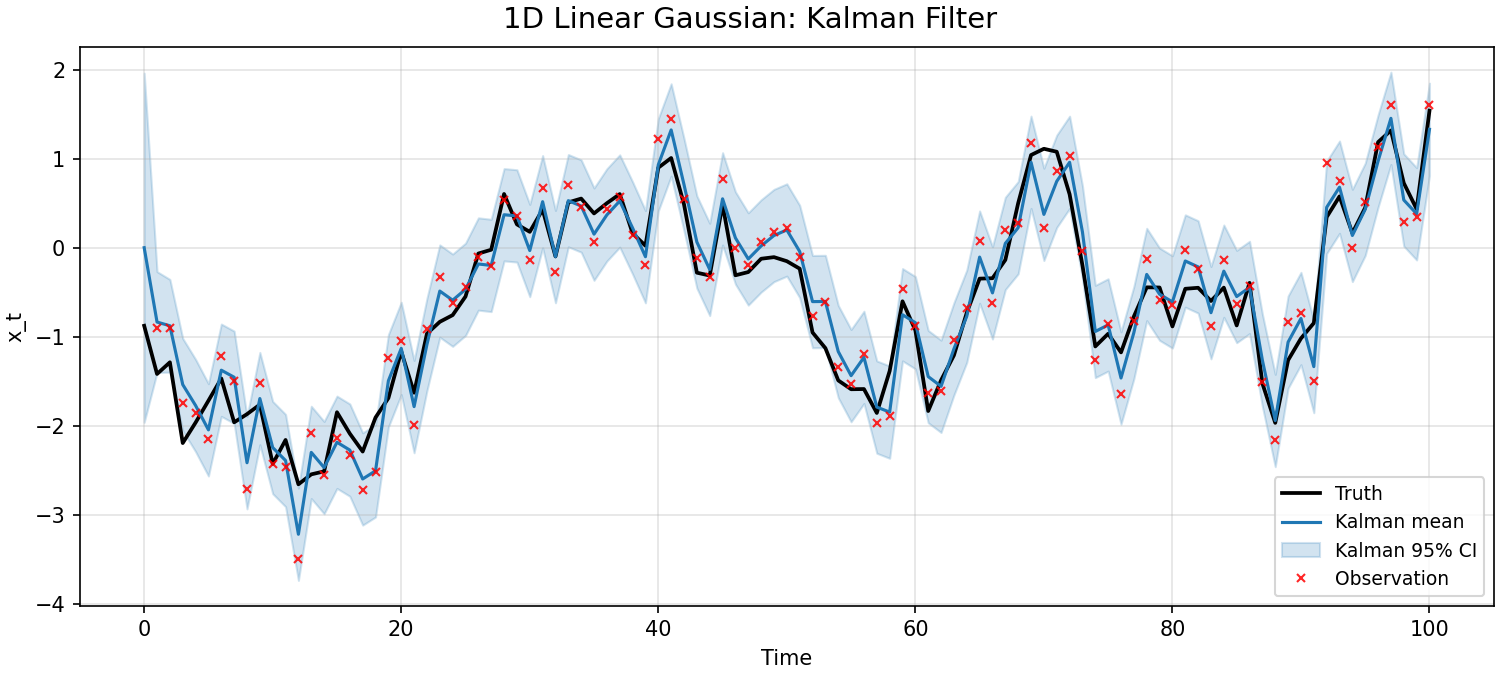
\includegraphics[width=0.75\linewidth]{kalman_1d_linear.png}
    \caption{Kalman filter on the 1D linear Gaussian model ($F = 0.95$, $B = 0.5$, $H = 1.0$, $D = 0.3$, $T = 100$, seed $42$). True state in black; Kalman posterior mean in blue with the $95\%$ credible band; observations shown as red crosses. RMSE $= 0.269$, log-likelihood $= -104.80$.}
    \label{fig:kalman-1d-linear}
\end{figure}

The run takes $1.03$ seconds on CPU ($10.3$ ms per time step, incremental peak memory $2.1$ MB, GPU unused); for a 1D state the entire filter reduces to two scalar updates per step, so the cost is essentially measurement noise in the timing --- a useful reference point against which the particle-filter wall times in Tables~\ref{tab:edh-rb}--\ref{tab:edh-sv-log} become meaningful.

\paragraph{What this plot is for.}
This is not a benchmark of Kalman's accuracy. The derivation in \S\ref{sec:kalman-algorithm} already shows the Kalman filter is analytically exact for linear Gaussian, so there is no approximation error to measure. The RMSE of $0.269$ is the sampling-level discrepancy between the filter's posterior mean and the true state realisation for this particular seed, and is bounded below by the posterior standard deviation the filter itself reports. The plot is for \emph{pipeline sanity}: data generation, filter invocation, state sampling from the prior, covariance tracking, Riccati convergence, metric collection, and I/O all run end-to-end without error and produce numbers consistent with the analytic reference. This is the minimum bar every downstream benchmark in \S\ref{sec:particle-methods-section} and \S\ref{sec:param-estimation} must clear --- and the same Kalman-exact model family is what \S\ref{sec:hmc-multichain-lg-kalman-family} uses to validate HMC. If HMC on that family recovers the Kalman posterior over the parameters, the differentiable pipeline is sound; if it does not, the fault lies in HMC, not in the filter or the test harness.

\newpage
\section{EKF and UKF}

Kalman fails once the update is no longer linear Gaussian. EKF and UKF are the two Gaussian approximations I use next \cite{Särkkä2013BayesianFilteringAndSmoothing}. They both incorporate nonlinear corrections in the observation model $\mathbf{h}(x)$ while keeping additive noise. Augmented EKF/UKF variants can handle non-additive noise \cite{Särkkä2013BayesianFilteringAndSmoothing}, but I do not need them here. The only non-additive noise model in this report is the 1-d stochastic volatility model, and I use a log-squared transform to put it into an additive-noise form.

\subsection{EKF}
EKF is a nonlinear improvement on KF. The goal is to preserve most of the KF algorithm. Nonlinearity breaks the linear structure of the model.
\begin{equation}
\begin{split}
\mathbf{\hat F} \mathbf{x}_{k-1}  &\rightarrow \mathbf{f}(\mathbf{x}_{k-1})  \\
\mathbf{\hat H} \mathbf{x}_{k}  &\rightarrow \mathbf{h}(\mathbf{x}_{k-1})
\end{split}
\end{equation}
Expand the prediction and observation model:
\begin{equation}
\begin{split}
\mathbf{f}(\mathbf{ x} -\mathbf{ m}_{k-1}) &\approx \mathbf{f}(\mathbf{ m}_{k-1}) + \frac{\partial \mathbf{f}}{\partial \mathbf{x}}\Big|_{\mathbf{m}_{k-1}} (\mathbf{x}-\mathbf{ m }_{k-1}) +\mathcal{O} ((\mathbf{x}-\mathbf{ m }_{k-1})^2 ) \\
\mathbf{h}(\mathbf{ x} -\mathbf{ m}^-_{k}) &\approx \mathbf{h}(\mathbf{ m}^-_{k}) + \frac{\partial \mathbf{h}}{\partial \mathbf{x}}\Big|_{\mathbf{m}^-_{k}} (\mathbf{x}-\mathbf{ m }^-_{k}) +\mathcal{O} ((\mathbf{x}-\mathbf{ m }_{k-1})^2 ) 
\end{split}
\end{equation}
By weak nonlinearity, I mean the regime where the second derivative term can be ignored. I expect this linear approximation to fail when the following two terms are comparable.
\begin{equation}
\begin{split}
\frac{\partial \mathbf{h}}{\partial \mathbf{x}}\Big|_{\mathbf{m}^-_{k}} (\mathbf{x}-\mathbf{ m }^-_{k}) \sim \frac{\partial^2 \mathbf{h}}{\partial \mathbf{x}^2}|_{\mathbf{m}^-_{k}} (\mathbf{x}-\mathbf{ m }_{k-1})^2 
\end{split}
\end{equation}
When linear approximation holds, I can use the Kalman filter algorithm by adding time dependence to the evolution and observation matrices.
\begin{equation}
\begin{split}
&\mathbf{F}_k \leftarrow \mathbf{f}(\mathbf{m}_{k-1}) \\
&\mathbf{H}_k \leftarrow \mathbf{h}(\mathbf{m}^-_{k})
\end{split}
\end{equation}


\begin{algorithm}[H]
\caption{Extended Kalman Filter (EKF)}
\begin{algorithmic}[1]
\REQUIRE Model: $\mathbf{x}_k = \mathbf{f}(\mathbf{x}_{k-1}) + \boldsymbol{\omega}_{k-1}$,
  $\mathbf{z}_k = \mathbf{h}(\mathbf{x}_k) + \mathbf{v}_k$,
  $\boldsymbol{\omega}_{k-1} \sim \mathcal{N}(\mathbf{0},\mathbf{Q})$,
  $\mathbf{v}_k \sim \mathcal{N}(\mathbf{0},\mathbf{R})$
\REQUIRE Initial: $\mathbf{m}_0, \mathbf{P}_0$ 
\FOR{$k = 1, 2, \ldots$}
  \STATE \textbf{Prediction}:
  \STATE $\mathbf{m}_k^{-} \leftarrow \mathbf{f}(\mathbf{m}_{k-1})$
  \STATE $\mathbf{F} \leftarrow \frac{\partial \mathbf{f}}{\partial \mathbf{x}}\Big|_{\mathbf{m}_{k-1}}$
  \STATE $\mathbf{P}_k^{-} \leftarrow \mathbf{F}\,\mathbf{P}_{k-1}\,\mathbf{F}^{\top} + \mathbf{Q}$
  \STATE \textbf{Update} :
  \STATE $\hat{\mathbf{z}} \leftarrow \mathbf{h}(\mathbf{m}_k^{-})$
  \STATE $\mathbf{H} \leftarrow \frac{\partial \mathbf{h}}{\partial \mathbf{x}}\Big|_{\mathbf{m}_k^{-}}$
  \STATE $\boldsymbol{\nu} \leftarrow \mathbf{z}_k - \hat{\mathbf{z}}$ \hfill (innovation)
  \STATE $\mathbf{S} \leftarrow \mathbf{H}\,\mathbf{P}_k^{-}\,\mathbf{H}^{\top} + \mathbf{R}$
  \STATE $\mathbf{K} \leftarrow \mathbf{P}_k^{-}\,\mathbf{H}^{\top}\,\mathbf{S}^{-1}$ \hfill (Kalman gain via Cholesky solve)
  \STATE $\mathbf{m}_k \leftarrow \mathbf{m}_k^{-} + \mathbf{K}\,\boldsymbol{\nu}$
  \STATE $\mathbf{P}_k \leftarrow (\mathbf{I} - \mathbf{K}\mathbf{H})\,\mathbf{P}_k^{-}\,(\mathbf{I} - \mathbf{K}\mathbf{H})^\top + \mathbf{K}\,\mathbf{R}\,\mathbf{K}^{\top}$ \hfill (Joseph form)
\ENDFOR
\end{algorithmic}
\end{algorithm}

\subsection{UKF}

The EKF approximates the nonlinear model by linearization, which requires computing the Jacobians $\mathbf{F}$ and $\mathbf{H}$. The UKF takes a different route: instead of approximating the \emph{function}, it approximates the \emph{distribution} that results from pushing a Gaussian through the function. The key observation is that the Kalman gain can be written without any reference to $\mathbf{H}$. In the linear case, $\mathbf{K} = \mathbf{P}\mathbf{H}^\top \mathbf{S}^{-1}$ and $\mathbf{z}_k^- = \mathbf{H}\mathbf{x}_k^- + \mathbf{v}_k$ with $\mathbf{v}_k \sim \mathcal{N}(\mathbf{0}, \mathbf{R})$ independent of $\mathbf{x}_k^-$. The cross-covariance between the predicted state and predicted observation is
\begin{equation}
\begin{split}
  \Cov(\mathbf{x}_k^-, \mathbf{z}_k^-)
  &= \mathbb{E}\!\left[(\mathbf{x}_k^{-} - \mathbf{m}_k^-)(\mathbf{z}_k^{-} - \mathbf{H}\mathbf{m}_k^-)^\top\right] \\
  &= \mathbb{E}\!\left[(\mathbf{x}_k^{-} - \mathbf{m}_k^-)\bigl(\mathbf{H}(\mathbf{x}_k^{-} - \mathbf{m}_k^-) + \mathbf{v}_k\bigr)^\top\right] \\
  &= \mathbb{E}\!\left[(\mathbf{x}_k^{-} - \mathbf{m}_k^-)(\mathbf{x}_k^{-} - \mathbf{m}_k^-)^\top\right]\mathbf{H}^\top \\
  &= \mathbf{P}_k^{-}\mathbf{H}^\top,
\end{split}
\end{equation}
where the cross term $\mathbb{E}[(\mathbf{x}_k^- - \mathbf{m}_k^-)\mathbf{v}_k^\top] = 0$ by independence. So $\mathbf{P}_k^-\mathbf{H}^\top = \Cov(\mathbf{x}_k^-, \mathbf{z}_k^-) \equiv \mathbf{P}_{xz}$. For the innovation covariance,
\begin{equation}
\begin{split}
  \Cov(\mathbf{z}_k^-, \mathbf{z}_k^-)
  &= \mathbb{E}\!\left[\bigl(\mathbf{H}(\mathbf{x}_k^{-} - \mathbf{m}_k^-) + \mathbf{v}_k\bigr)\bigl(\mathbf{H}(\mathbf{x}_k^{-} - \mathbf{m}_k^-) + \mathbf{v}_k\bigr)^\top\right] \\
  &= \mathbf{H}\,\mathbb{E}\!\left[(\mathbf{x}_k^{-} - \mathbf{m}_k^-)(\mathbf{x}_k^{-} - \mathbf{m}_k^-)^\top\right]\mathbf{H}^\top + \mathbb{E}[\mathbf{v}_k\mathbf{v}_k^\top] \\
  &= \mathbf{H}\mathbf{P}_k^{-}\mathbf{H}^\top + \mathbf{R} \;=\; \mathbf{S},
\end{split}
\end{equation}
where the cross terms again vanish by independence. So $\Cov(\mathbf{z}_k^-, \mathbf{z}_k^-) \equiv \mathbf{P}_{zz} = \mathbf{S}$. The Kalman gain therefore takes the equivalent form
\begin{equation}
  \mathbf{K} = \mathbf{P}_{xz}\,\mathbf{S}^{-1},
  \label{eq:kalman-gain-cov}
\end{equation}
and this expression makes no assumption about linearity and is "blind" to the functional form of the models. If I can estimate $\mathbf{P}_{xz}$ and $\mathbf{S}$ for a nonlinear $\mathbf{h}$, I can run the Kalman update as-is.

The question is how to compute these covariances when $\mathbf{h}$ is nonlinear. EKF evaluates them analytically via the Jacobian and discards higher-order terms. UKF instead draws $2d+1$ \emph{sigma points} deterministically from the predicted Gaussian $\mathcal{N}(\mathbf{m}_k^-, \mathbf{P}_k^-)$, propagates each through $\mathbf{h}$, and computes the covariances as weighted sums:
\begin{align}
  \hat{\mathbf{z}} &= \sum_j W_m^{(j)}\,\mathbf{h}(\boldsymbol{\chi}_j), \\
  \mathbf{S} &= \sum_j W_c^{(j)}\,(\mathbf{h}(\boldsymbol{\chi}_j) - \hat{\mathbf{z}})(\mathbf{h}(\boldsymbol{\chi}_j) - \hat{\mathbf{z}})^\top + \mathbf{R}, \\
  \mathbf{P}_{xz} &= \sum_j W_c^{(j)}\,(\boldsymbol{\chi}_j - \mathbf{m}_k^-)(\mathbf{h}(\boldsymbol{\chi}_j) - \hat{\mathbf{z}})^\top.
\end{align}
The sigma points are chosen so that their weighted mean and covariance exactly match the Gaussian $\mathcal{N}(\mathbf{m}_k^-, \mathbf{P}_k^-)$, which guarantees the approximation is at least second-order accurate (capturing the curvature of $\mathbf{h}$ that EKF misses). No Jacobian is required. With $\mathbf{P}_{xz}$ and $\mathbf{S}$ in hand, the rest of the update is identical to the Kalman filter.

Here $d$ is the \emph{state dimension}. The number of sigma points $2d+1$ is fixed by the method --- one at the mean, $d$ pairs placed symmetrically along each column of $\sqrt{(d+\lambda)\mathbf{P}}$. 

The three tuning parameters $\alpha, \beta, \kappa$ all feed into the composite scaling parameter $\lambda = \alpha^2(d + \kappa) - d$. The sigma point displacement is $h = \sqrt{(d+\lambda)\mathbf{P}}$, so $\lambda$ directly sets the spread. $\alpha \in (0,1]$ is the primary knob. The typical default $\alpha = 10^{-3}$ with $\kappa = 0$ gives $\lambda \approx -d$, so $(d+\lambda) \approx \alpha^2 d \approx 0$ --- the sigma points collapse nearly to the mean and the filter degenerates toward a linearization. $\kappa$ is minor and usually left at zero.

$\beta$ enters only in $W_c^{(0)} = W_m^{(0)} + (1 - \alpha^2 + \beta)$, adjusting how much the central sigma point contributes to the covariance. To see why $\beta = 2$ is optimal for Gaussians, consider the simplest case: $d = 1$, $f(x) = x^2$, $x \sim \mathcal{N}(0, P)$. The true variance is $\mathrm{Var}[x^2] = 3P^2 - P^2 = 2P^2$ (Gaussian fourth moment $\mathbb{E}[x^4] = 3P^2$). With $\kappa = 0$, let $h^2 = (1+\lambda)P$; the three sigma points give $f(\chi_j) \in \{0, h^2, h^2\}$. The UKF mean $\hat{z} = 2W_m^{(1)}h^2 = P$ is already exact. The covariance estimate is
\begin{equation}
  \widehat{\mathrm{Var}} = W_c^{(0)}(0 - P)^2 + 2W_c^{(1)}(h^2 - P)^2 = \left(W_c^{(0)} + \frac{\lambda^2}{1+\lambda}\right)P^2.
\end{equation}
Setting this equal to $2P^2$ requires $W_c^{(0)} + \lambda^2/(1+\lambda) = 2$. Substituting $W_c^{(0)} = \lambda/(1+\lambda) + (1-\alpha^2+\beta)$ and $\lambda = \alpha^2 - 1$ (for $d=1$, $\kappa=0$):
\begin{equation}
  (\alpha^2 - 1) + (1 - \alpha^2 + \beta) = 2 \;\Longrightarrow\; \beta = 2.
\end{equation}
The $\alpha^2$ terms cancel exactly, so $\beta = 2$ holds for any $\alpha$ when $d=1$, $\kappa=0$. For $d > 1$ the cancellation is approximate, but $\beta = 2$ remains a good default. 
\begin{algorithm}[H]
\caption{Unscented Kalman Filter (UKF)}
\begin{algorithmic}[1]
\REQUIRE Same model as EKF. UKF parameters: $\alpha, \beta, \kappa$; $\lambda = \alpha^2(d+\kappa)-d$
\REQUIRE UKF weights: $W_m^{(0)} = \frac{\lambda}{d+\lambda}$, $W_c^{(0)} = W_m^{(0)} + 1 - \alpha^2 + \beta$, $W_m^{(j)} = W_c^{(j)} = \frac{1}{2(d+\lambda)}$ for $j=1,\ldots,2d$
\FOR{$k = 1, 2, \ldots$}
  \STATE \textbf{Prediction}:
  \STATE Generate $2d+1$ sigma points: $\boldsymbol{\chi}_0 = \mathbf{m}_{k-1}$
  \STATE $\boldsymbol{\chi}_j = \mathbf{m}_{k-1} + \left[\sqrt{(d+\lambda)\mathbf{P}_{k-1}}\right]_j$, \quad $j=1,\ldots,d$
  \STATE $\boldsymbol{\chi}_{d+j} = \mathbf{m}_{k-1} - \left[\sqrt{(d+\lambda)\mathbf{P}_{k-1}}\right]_j$, \quad $j=1,\ldots,d$
  \STATE Propagate: $\boldsymbol{\chi}_j^{*} \leftarrow \mathbf{f}(\boldsymbol{\chi}_j)$ for all $j$
  \STATE $\mathbf{m}_k^{-} \leftarrow \sum_{j=0}^{2d} W_m^{(j)}\, \boldsymbol{\chi}_j^{*}$
  \STATE $\mathbf{P}_k^{-} \leftarrow \sum_{j=0}^{2d} W_c^{(j)} (\boldsymbol{\chi}_j^{*} - \mathbf{m}_k^{-})(\boldsymbol{\chi}_j^{*} - \mathbf{m}_k^{-})^\top + \mathbf{Q}$
  \STATE \textbf{Update} (for each particle $i$):
  \STATE Regenerate sigma points from $(\mathbf{m}_k^{-}, \mathbf{P}_k^{-})$
  \STATE Propagate through observation: $\boldsymbol{\gamma}_j \leftarrow \mathbf{h}(\boldsymbol{\chi}_j)$
  \STATE $\hat{\mathbf{z}} \leftarrow \sum_{j=0}^{2d} W_m^{(j)} \boldsymbol{\gamma}_j$
  \STATE $\mathbf{S} \leftarrow \sum_{j=0}^{2d} W_c^{(j)} (\boldsymbol{\gamma}_j - \hat{\mathbf{z}})(\boldsymbol{\gamma}_j - \hat{\mathbf{z}})^\top + \mathbf{R}$
  \STATE $\mathbf{P}_{xz} \leftarrow \sum_{j=0}^{2d} W_c^{(j)} (\boldsymbol{\chi}_j - \mathbf{m}_k^{-})(\boldsymbol{\gamma}_j - \hat{\mathbf{z}})^\top$
  \STATE $\mathbf{K} \leftarrow \mathbf{P}_{xz}\,\mathbf{S}^{-1}$ \hfill (Kalman gain via Cholesky solve)
  \STATE $\mathbf{m}_k \leftarrow \mathbf{m}_k^{-} + \mathbf{K}(\mathbf{z}_k - \hat{\mathbf{z}})$
  \STATE $\mathbf{P}_k \leftarrow \mathbf{P}_k^{-} - \mathbf{K}\mathbf{P}_{xz}^{\top} - \mathbf{P}_{xz}\mathbf{K}^{\top} + \mathbf{K}\mathbf{S}\mathbf{K}^{\top}$
\ENDFOR
\end{algorithmic}
\end{algorithm}
%\paragraph{Parameter choice for the SV model.} The 1D stochastic volatility model has $d = 1$, so there are always 3 sigma points. With the default $\alpha = 10^{-3}$, $\kappa = 0$: $\lambda \approx -1$, giving $(d+\lambda) \approx 10^{-6}$ --- sigma points essentially at the mean, which is too tight for $h(x) = e^{x/2}$. A better choice is $\alpha = 1$, which gives $\lambda = 0$ and places sigma points at $m_k^- \pm \sqrt{P_k^-}$, covering one standard deviation of the predicted distribution and capturing the relevant curvature of $e^{x/2}$. $\beta = 2$ and $\kappa = 0$ are kept as defaults. {\color{red} add experiments for this}

\subsection{EKF/UKF on non-linear models}
\label{sec:ekf-ukf-nonlinear}
I use two nonlinear test models here: range-bearing and 1-d stochastic volatility. They first appear here and then carry through the later particle-filter and HMC sections.

\paragraph{Range bearing model.}
\label{par:range-bearing-model}
The state $\mathbf{x}_t = (x_t, y_t)^\top \in \mathbb{R}^2$ represents a 2D position. The state evolves linearly and observations are nonlinear range-bearing measurements from a sensor at position $(x_s, y_s)^\top$. The state transition is
\begin{equation}
    \mathbf{x}_t = F\,\mathbf{x}_{t-1} + \mathbf{w}_t, \qquad
    \mathbf{w}_t \sim \mathcal{N}(\mathbf{0},\, Q),
\end{equation}
where $F = I_2$ (constant-position model) and $Q = 0.01\,I_2$. The observation model is
\begin{equation}
    \mathbf{z}_t = h(\mathbf{x}_t) + \mathbf{v}_t, \qquad
    \mathbf{v}_t \sim \mathcal{N}(\mathbf{0},\, R),
\end{equation}
with the nonlinear measurement function
\begin{equation}
    h(\mathbf{x}) =
    \begin{pmatrix}
        \sqrt{(x - x_s)^2 + (y - y_s)^2} \\[4pt]
        \operatorname{atan2}(y - y_s,\; x - x_s)
    \end{pmatrix},
\end{equation}
and diagonal observation noise covariance $R = \operatorname{diag}(\sigma_r^2,\, \sigma_b^2)$, where $\sigma_r = 0.1$ (range noise std.) and $\sigma_b = 0.1\,\mathrm{rad}$ (bearing noise std.). The sensor is located at the origin $(x_s, y_s) = (0, 0)$. The initial distribution is $\mathbf{x}_0 \sim \mathcal{N}(\boldsymbol{\mu}_0,\, \Sigma_0)$ with $\boldsymbol{\mu}_0 = (5, 5)^\top$ and $\Sigma_0 = I_2$.

The choice $\boldsymbol{\mu}_0 = (5, 5)^\top$ is not arbitrary: it is the direct application of the cross-cutting initial-condition principle stated in \S\ref{par:init-conditions} to a model with a singular observation Jacobian. The range function $h_1(\mathbf{x}) = \sqrt{(x - x_s)^2 + (y - y_s)^2}$ has a gradient $\partial h_1/\partial \mathbf{x} = (\mathbf{x} - \mathbf{x}_s)/\lVert \mathbf{x} - \mathbf{x}_s\rVert$ that is undefined at the sensor position $\mathbf{x} = \mathbf{x}_s = (0,0)$, and the bearing function $h_2(\mathbf{x}) = \operatorname{atan2}(y - y_s, x - x_s)$ has a gradient $\partial h_2/\partial \mathbf{x} = (-(y-y_s), x-x_s)/\lVert \mathbf{x} - \mathbf{x}_s\rVert^2$ that \emph{diverges} at the sensor as $1/\lVert \mathbf{x} - \mathbf{x}_s\rVert^2$. Any prior whose mean sits close to the origin --- for example $\boldsymbol{\mu}_0 = (1, 1)^\top$, which places the mean at distance $\sqrt{2} \approx 1.41$ from the sensor --- gives a bearing-Jacobian magnitude of order $1/2$ and a range-Jacobian direction that flips sign rapidly across the origin, so the EKF/UKF linearisation at the first time step is poorly conditioned and the particle filters sample many particles into the near-singular region. Moving the prior mean out to $(5, 5)^\top$ (distance $5\sqrt{2} \approx 7.07$ from the sensor) shrinks the bearing-Jacobian magnitude to order $1/50$, keeps $\Sigma_0 = I_2$ well inside the smoothly-observable region, and makes every downstream filter's first-step linearisation stable. 

\paragraph{Stochastic volatility model.}
The latent state $x_t \in \mathbb{R}$ represents the log-volatility. The state transition is
\begin{equation}
    x_t = \alpha\, x_{t-1} + \sigma\, w_t, \qquad w_t \sim \mathcal{N}(0, 1),
\end{equation}
with persistence parameter $\alpha = 0.91$ and volatility-of-volatility $\sigma = 1.0$. Since $|\alpha| < 1$, the process is stationary, and I initialize $x_0 \sim \mathcal{N}\!\left(0,\, \sigma^2/(1-\alpha^2)\right)$ from its stationary distribution, following the same principle discussed for the 1-D Kalman filter in Section~\ref{sec:kalman-algorithm}. The observation model is
\begin{equation}
    y_t = \beta\,\exp\!\left(\tfrac{x_t}{2}\right) v_t, \qquad v_t \sim \mathcal{N}(0, 1),
\end{equation}
with scale parameter $\beta = 0.5$. The density $p(y_t \mid x_t) = \mathcal{N}(0,\, \beta^2 e^{x_t})$, so the observation noise is multiplicative and the likelihood is non-Gaussian in $x_t$. It is straightforward to run EKF and UKF on the range bearing model. Stochastic volatility is harder because the multiplicative noise means the observation is not a function of $x_t$ alone in the additive sense EKF/UKF assume. To make EKF/UKF applicable, I apply a log-squared transform $z_t = \log y_t^2$ to the observation, which yields
\begin{equation}
    z_t = \log\beta^2 + x_t + \varepsilon_t,
\end{equation}
where $\varepsilon_t = \log v_t^2 \sim \log\chi^2_1$ is approximated as $\mathcal{N}(\mu_\varepsilon,\, \sigma_\varepsilon^2)$ with $\mu_\varepsilon = \psi(1/2) + \log 2 \approx -1.2704$ and $\sigma_\varepsilon^2 = \pi^2/2 \approx 4.935$, where $\psi$ is the digamma function. This linearises the observation in $x_t$ and puts the model into the additive-noise form EKF/UKF require.

\paragraph{Numerical results.} All six experiments below share seed $42$, $T = 100$ time steps, and 64-bit precision. UKF uses the defaults $\alpha = 10^{-3}$, $\beta = 2$, $\kappa = 0$.
\begin{itemize}
\item
On the range-bearing model, both EKF (RMSE $= 0.133$, log-likelihood $= +109.90$) and UKF (RMSE $= 0.133$, log-likelihood $= +109.89$) track the state accurately (Figure~\ref{fig:ekf-ukf-rb}). The nonlinearity here is mild --- $h$ is smooth away from the sensor and the posterior stays well inside a region where the linearisation is accurate --- so EKF and UKF produce essentially identical estimates.
\item
On the raw stochastic volatility model, applying EKF/UKF directly with the nonlinear measurement $y_t = \beta e^{x_t/2} v_t$ gives RMSE $= 2.04$ for both filters (Figure~\ref{fig:ekf-ukf-sv-raw}). The Jacobian $\partial h / \partial x_t = (\beta/2)\, e^{x_t/2} v_t$ depends on the noise realisation $v_t$, so the EKF linearisation is not even well-defined in the usual additive-noise sense, and both filters mostly track the prior mean rather than responding to observations. Applying the log-squared transform (Figure~\ref{fig:ekf-ukf-sv-log}) drops the RMSE to $1.14$, nearly halving the latent-state error and recovering meaningful volatility tracking. Log-likelihoods for raw and log-transformed runs are not directly comparable because they are computed in different observation spaces ($y_t$ versus $\log y_t^2$); only the RMSE in latent-$x_t$ space is a fair comparison. EKF and UKF are numerically indistinguishable on the 1D SV model in both forms.
\end{itemize}

\paragraph{Computational footprint.} All six runs execute on CPU; the EKF/UKF machinery has no meaningful GPU workload at $d_x \le 2$ and $T = 100$. Table~\ref{tab:ekf-ukf-footprint} reports wall time and memory for all six runs. The numbers below are measured on the same host as the Kalman demo in \S\ref{sec:kalman-algorithm} and should be read as a reference point for the particle-filter wall times in Tables~\ref{tab:edh-rb}--\ref{tab:edh-sv-log}, not as an optimisation target.

\begin{table}[H]
\centering
\footnotesize
\caption{EKF/UKF runtime and memory footprint. Peak memory is the incremental peak during the filter run (measured in Python's resident set). $d_x$ is the latent state dimension; $d_z$ is the observation dimension. All six runs are CPU-only; no GPU memory consumed.}
\label{tab:ekf-ukf-footprint}
\begin{tabular}{lccccc}
\toprule
Experiment & $d_x$ / $d_z$ & Wall (s) & Time/step (ms) & Peak mem (MB) \\
\midrule
Range-bearing EKF           & $2$ / $2$ & $1.75$ & $17.5$ & $2.4$ \\
Range-bearing UKF           & $2$ / $2$ & $1.88$ & $18.8$ & $2.8$ \\
SV raw EKF                  & $1$ / $1$ & $1.71$ & $17.1$ & $2.5$ \\
SV raw UKF                  & $1$ / $1$ & $1.90$ & $18.9$ & $3.0$ \\
SV log-transform EKF        & $1$ / $1$ & $1.73$ & $17.3$ & $2.5$ \\
SV log-transform UKF        & $1$ / $1$ & $1.95$ & $19.5$ & $3.0$ \\
\bottomrule
\end{tabular}
\end{table}

UKF is consistently $5$--$15\%$ slower than EKF per step. The gap is explained entirely by the sigma-point propagation cost: UKF passes $2d_x + 1 = 5$ sigma points (RB) or $3$ sigma points (SV) through the observation function at every step, whereas EKF analytically evaluates a single Jacobian. On these small-$d_x$ problems the absolute cost is trivial ($\sim 1$--$2$ ms per step extra), but the ratio is consistent across models and foreshadows the sigma-point scaling $\mathcal{O}(d_x)$ that makes UKF less attractive as state dimension grows. Peak memory is essentially noise ($\sim 2$--$3$ MB) --- the filters hold only the current mean, covariance, and a handful of scratch matrices.

\begin{figure}[H]
    \centering
    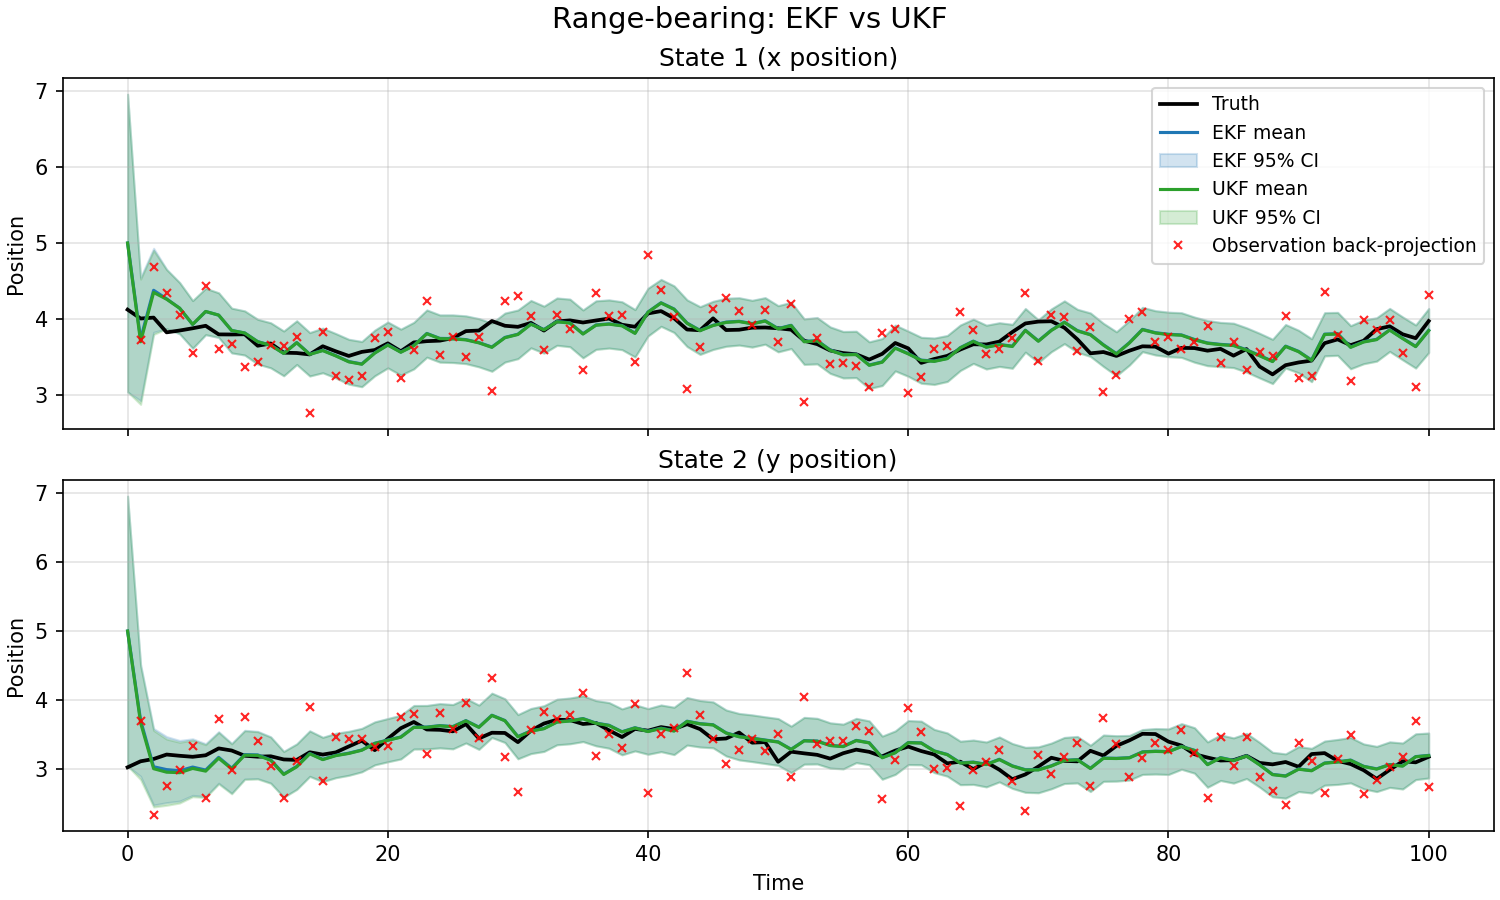
\includegraphics[width=0.85\linewidth]{ekf_ukf_range_bearing_combined.png}
    \caption{Range-bearing: EKF (blue) and UKF (green) overlaid on the truth trajectory (black), with back-projected observations shown as red crosses. Both filters reach RMSE $\approx 0.133$ and are numerically indistinguishable.}
    \label{fig:ekf-ukf-rb}
\end{figure}

\begin{figure}[H]
    \centering
    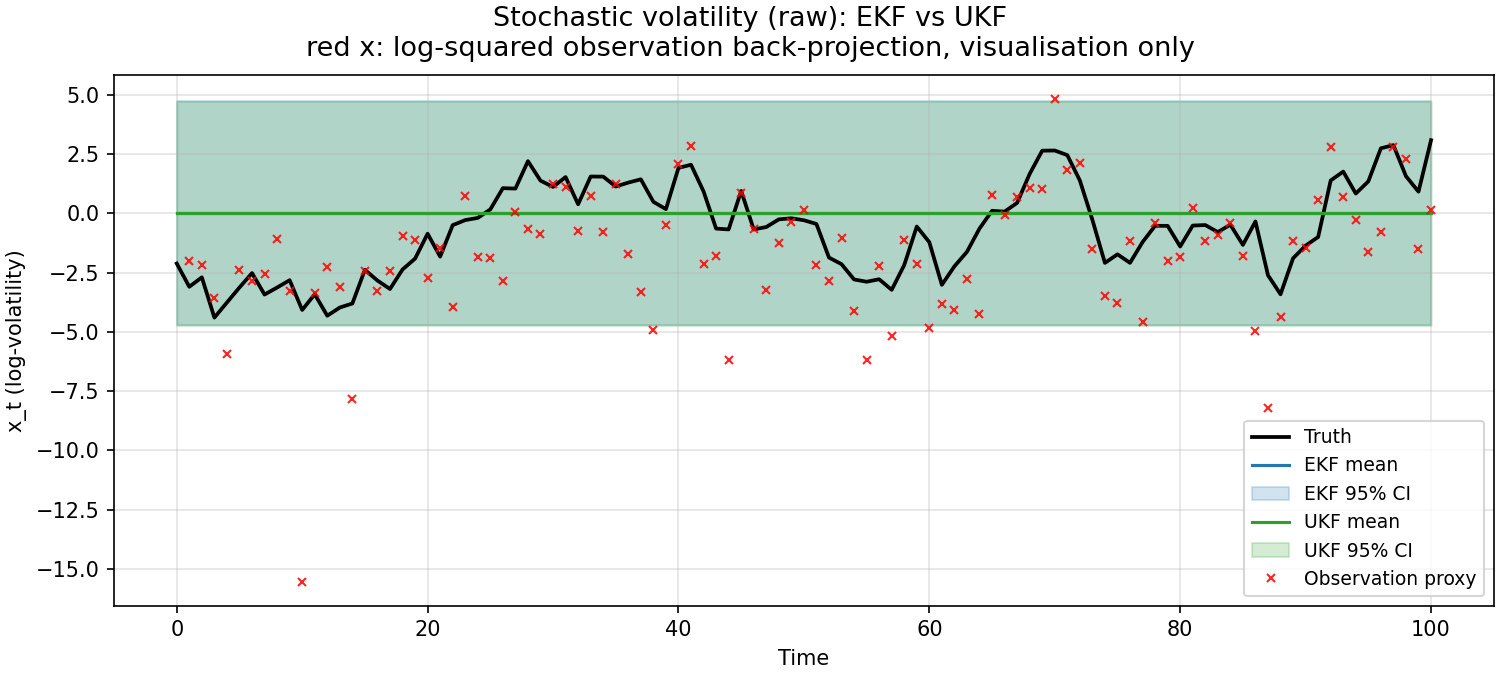
\includegraphics[width=0.85\linewidth]{ekf_ukf_sv_raw_combined.png}
    \caption{Raw stochastic volatility: EKF (blue) and UKF (green) both mostly track the prior mean rather than the latent volatility. Both filters have RMSE $= 2.04$ and log-likelihood $= -151.20$ in the raw observation space.}
    \label{fig:ekf-ukf-sv-raw}
\end{figure}

\begin{figure}[H]
    \centering
    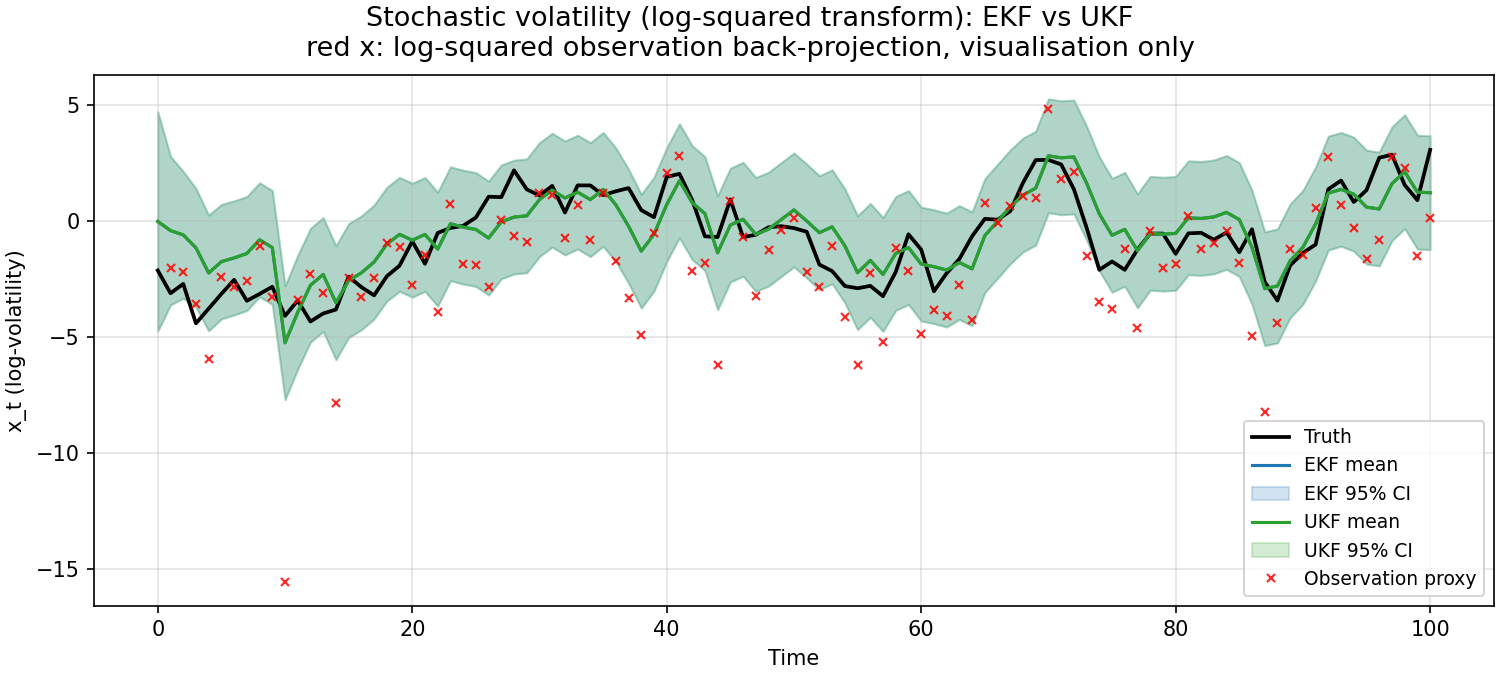
\includegraphics[width=0.85\linewidth]{ekf_ukf_sv_log_combined.png}
    \caption{Log-squared stochastic volatility: EKF (blue) and UKF (green) recover meaningful latent-volatility tracking after the transform. Both filters have RMSE $= 1.14$ and log-likelihood $= -235.27$ in the transformed observation space.}
    \label{fig:ekf-ukf-sv-log}
\end{figure}



%%%%%%%%%%%%%%%%%%%%%%%%%%%%%%%%%%%%%%%%%%%%%%%%%%%%%%%%%%
\newpage
\section{Particle-Based Methods}
\label{sec:particle-methods-section}

\subsection{Importance Sampling and Sequential Monte Carlo}
Start from the filtering recursion.
\begin{equation}
\begin{split}
   \textbf{Prediction: } & \quad p(x_k \mid z_{1:k-1}) = \int p(x_k \mid x_{k-1}) \, p(x_{k-1} \mid z_{1:k-1}) \, dx_{k-1} \\[1ex]
   \textbf{Update: }     & \quad p(x_k \mid z_{1:k}) = \frac{p(z_k \mid x_k) \, p(x_k \mid z_{1:k-1})}{p(z_k \mid z_{1:k-1})},
\end{split}
\end{equation}
are intractable in general because the prediction integral has no closed form when $f$ or $h$ are nonlinear or the noise is non-Gaussian, and the normalization constant $p(z_k \mid z_{1:k-1})$ in the update is itself an integral over all of state space. The key idea of particle-based methods is to \textit{represent the filtering distribution by a set of weighted samples} (particles). Given $N$ particles $\{x_k^{(i)}\}_{i=1}^N$ with associated weights $\{w_k^{(i)}\}_{i=1}^N$ satisfying $\sum_i w_k^{(i)} = 1$, we approximate
\begin{equation}
    p(x_k \mid z_{1:k}) \approx \sum_{i=1}^N w_k^{(i)} \, \delta\!\left(x_k - x_k^{(i)}\right).
\end{equation}
With this empirical representation, any posterior expectation reduces to a weighted sum,
\begin{equation}
    \mathbb{E}[g(x_k) \mid z_{1:k}] = \int g(x_k)\, p(x_k \mid z_{1:k})\, dx_k \approx \sum_{i=1}^N w_k^{(i)}\, g\!\left(x_k^{(i)}\right),
\end{equation}
so recovering the posterior mean and covariance requires no further integration.

\subsubsection*{Importance Sampling}

The challenge is that we generally cannot sample directly from the target $p(x_k \mid z_{1:k})$.
\textit{Importance sampling} (IS) resolves this by drawing from a tractable \textit{proposal distribution} $q(x_k)$ and correcting for the mismatch with weights. For any function $g$,
\begin{equation}
    \mathbb{E}_{p}[g(x_k)] = \int g(x_k)\, \frac{p(x_k \mid z_{1:k})}{q(x_k)}\, q(x_k)\, dx_k \approx \sum_{i=1}^N w^{(i)}\, g\!\left(x_k^{(i)}\right), \quad x_k^{(i)} \sim q(x_k),
\end{equation}
where the \textit{importance weight} is proportional to the ratio $w^{(i)} \propto p(x_k^{(i)} \mid z_{1:k}) / q(x_k^{(i)})$. Since $p(x_k \mid z_{1:k})$ is known only up to a normalizing constant, I use the \textit{self-normalized} estimator with unnormalized weights $\tilde{w}^{(i)} \propto p(x_k^{(i)} \mid z_{1:k}) / q(x_k^{(i)})$,
\begin{equation}
    w_k^{(i)} = \frac{\tilde{w}_k^{(i)}}{\displaystyle\sum_{j=1}^N \tilde{w}_k^{(j)}}.
\end{equation}
This is consistent as $N \to \infty$ for any proposal $q$ with support containing that of $p$.

\subsubsection*{Sequential Monte Carlo}

Sequential use is where importance sampling becomes a filter. Suppose at time $k-1$ I hold a particle approximation $\{x_{k-1}^{(i)}, w_{k-1}^{(i)}\}$ of $p(x_{k-1} \mid z_{1:k-1})$. The \textit{only} goal at time $k$ is the posterior $p(x_k \mid z_{1:k})$, whose mean $m_k$ and covariance $P_k$ are the quantities of interest. The intermediate predicted distribution $p(x_k \mid z_{1:k-1})$ and its moments $m_k^-$, $P_k^-$ are not ends in themselves—they are merely one route to the posterior. This gives me great freedom: I may draw new particles from \textit{any} proposal
\begin{equation}
    x_k^{(i)} \sim q(x_k \mid x_{k-1}^{(i)}, z_k), \qquad i = 1, \ldots, N,
\end{equation}
provided it has sufficient support, and correct for the mismatch via IS weights. Writing the target as $p(x_k \mid z_{1:k}) \propto p(z_k \mid x_k)\, p(x_k \mid x_{k-1}^{(i)})$, the unnormalized weight for each particle is
\begin{equation}
    \tilde{w}_k^{(i)} = w_{k-1}^{(i)} \cdot \frac{p(z_k \mid x_k^{(i)})\, p(x_k^{(i)} \mid x_{k-1}^{(i)})}{q(x_k^{(i)} \mid x_{k-1}^{(i)}, z_k)},
    \label{eq:smc_weight}
\end{equation}
which after normalization gives $p(x_k \mid z_{1:k}) \approx \sum_i w_k^{(i)}\, \delta(x_k - x_k^{(i)})$. This is the \textit{Sequential Monte Carlo} (SMC) framework: the prediction and update integrals are handled together in a single IS step, and the two-step predict-then-update decomposition of the Kalman family is not fundamental here—it is just one way to factor the joint density.

The proposal is the design choice. The simplest option $q(x_k \mid x_{k-1}^{(i)}, z_k) = p(x_k \mid x_{k-1}^{(i)})$ ignores the current observation entirely, simplifying~\eqref{eq:smc_weight} to $\tilde{w}_k^{(i)} \propto w_{k-1}^{(i)} \cdot p(z_k \mid x_k^{(i)})$—this is the Bootstrap Particle Filter. More sophisticated methods either use a smarter proposal that already incorporates $z_k$ (while still relying on weights to correct for the approximation), or abandon importance weights altogether and instead move particles deterministically toward the posterior using a flow constructed from a Gaussian approximation to $p(x_k \mid z_{1:k})$—as in the EDH and LEDH flow filters described later.

A well-known practical issue with weighted SMC is \textit{weight degeneracy}: after many steps, the multiplicative weight update concentrates nearly all weight on very few particles. The standard remedy is \textit{resampling}, and I study its effect by applying Bootstrap Particle Filter on non-linear models.

\subsection{Bootstrap Particle Filter}

\subsubsection{Algorithm}

The BPF is the simplest instantiation of SMC: the proposal is the transition prior $q = p(x_k \mid x_{k-1}^{(i)})$, so each particle is propagated by forward-simulating the dynamics and scored against the new observation. From~\eqref{eq:smc_weight} the weight reduces to $\tilde{w}_k^{(i)} \propto w_{k-1}^{(i)} \cdot p(z_k \mid x_k^{(i)})$.

\begin{algorithm}[H]
\caption{Bootstrap Particle Filter (BPF)}
\label{alg:bpf}
\begin{algorithmic}[1]
\REQUIRE particles $\{x_{k-1}^{(i)},\, w_{k-1}^{(i)}\}_{i=1}^N$, observation $z_k$
\FOR{$i = 1$ \textbf{to} $N$}
    \STATE \textbf{Predict:} sample $x_k^{(i)} \sim p(x_k \mid x_{k-1}^{(i)})$
    \STATE \textbf{Weight:} $\tilde{w}_k^{(i)} \leftarrow w_{k-1}^{(i)} \cdot p(z_k \mid x_k^{(i)})$
\ENDFOR
\STATE \textbf{Normalize:} $w_k^{(i)} \leftarrow \tilde{w}_k^{(i)} \big/ \sum_{j=1}^N \tilde{w}_k^{(j)}$ for all $i$
\STATE \textbf{Estimate:} $m_k = \sum_i w_k^{(i)}\, x_k^{(i)}$, \quad $P_k = \sum_i w_k^{(i)}\bigl(x_k^{(i)}-m_k\bigr)\bigl(x_k^{(i)}-m_k\bigr)^\top$
\IF{$N_{\mathrm{eff}} = \bigl(\sum_i (w_k^{(i)})^2\bigr)^{-1} < N/2$}
    \STATE \textbf{Resample} (Algorithm~\ref{alg:systematic}); set $w_k^{(i)} \leftarrow 1/N$ for all $i$
\ENDIF
\ENSURE $\{x_k^{(i)},\, w_k^{(i)}\}_{i=1}^N \approx p(x_k \mid z_{1:k})$, moments $m_k$, $P_k$
\end{algorithmic}
\end{algorithm}

\subsubsection{Particle Degeneracy and Resampling}

The weight update multiplies by a per-particle likelihood, and repeated multiplication concentrates the relative mass on a shrinking number of particles. This is the degeneracy mechanism: not that likelihood factors are below one (they are not bounded for density functions), but that the distribution of relative weights collapses exponentially fast with time. The \textit{effective sample size}
\begin{equation}
    N_{\mathrm{eff}} = \frac{1}{\displaystyle\sum_{i=1}^N \bigl(w_k^{(i)}\bigr)^2}
\end{equation}
quantifies this: it equals $N$ when all weights are uniform and drops toward $1$ at full collapse. I trigger resampling when $N_{\mathrm{eff}} < N/2$.

\paragraph{Multinomial resampling.}
The conceptually simplest fix draws $N$ independent samples from the categorical distribution defined by the current weights,
\begin{equation}
    x_k^{(i)} \sim \mathrm{Categorical}\!\bigl(\{w_k^{(j)}\}_{j=1}^N\bigr), \quad i = 1, \ldots, N,
\end{equation}
then resets all weights to $1/N$. High-weight particles are duplicated; low-weight ones are discarded. While unbiased, this introduces additional Monte Carlo variance: because each draw is independent, particles with moderate weight may be selected zero times by chance. The cost is $O(N \log N)$ via the inverse-CDF method.

\paragraph{Systematic resampling (the actual implementation).}
I use systematic resampling, which addresses both drawbacks. A single draw $u \sim \mathcal{U}(0,\,1/N)$ places $N$ evenly-spaced points across $[0, 1]$:
\begin{equation}
    u^{(i)} = u + \frac{i-1}{N}, \quad i = 1, \ldots, N.
\end{equation}
Particle $j$ is selected for slot $i$ if $u^{(i)}$ falls in $\bigl(\sum_{l < j} w_k^{(l)},\, \sum_{l \leq j} w_k^{(l)}\bigr]$. Because the grid is deterministically spread over $[0,1]$, every particle with weight $w^{(j)} > 1/N$ is guaranteed to appear at least $\lfloor N w^{(j)} \rfloor$ times, and the copy count deviates from the ideal $N w^{(j)}$ by at most 1. This eliminates the random clustering of multinomial resampling, minimizes the variance of the resampling step, and reduces the cost to $O(N)$ via a single linear pass through the cumulative weight sum.

\begin{algorithm}[H]
\caption{Systematic Resampling}
\label{alg:systematic}
\begin{algorithmic}[1]
\REQUIRE weights $\{w^{(i)}\}_{i=1}^N$, positions $\{x^{(i)}\}_{i=1}^N$
\STATE Draw $u \sim \mathcal{U}(0,\, 1/N)$; set $u^{(i)} = u + (i-1)/N$ for $i = 1,\ldots,N$
\STATE Compute cumulative sums $C_j = \sum_{l=1}^{j} w^{(l)}$
\FOR{$i = 1$ \textbf{to} $N$}
    \STATE Find $j_i$ such that $C_{j_i-1} < u^{(i)} \leq C_{j_i}$;\; set $\bar{x}^{(i)} \leftarrow x^{(j_i)}$
\ENDFOR
\ENSURE $\{\bar{x}^{(i)},\, 1/N\}_{i=1}^N$
\end{algorithmic}
\end{algorithm}

After resampling the particle set has uniform weights and represents the same distribution as before, but with diversity restored. The cost is \textit{sample impoverishment}: multiplicity alone now encodes the distribution, with no weight diversity. This motivates the flow-based methods described next, which avoid resampling altogether by moving particles directly toward the posterior. I applied the bootstrap particle filter to the same range-bearing and stochastic-volatility models. Figure~\ref{fig:particle_tracking} shows the posterior mean tracking. Figure~\ref{fig:ess_time} shows that the range-bearing ESS collapses within the first few steps, while stochastic volatility stays above threshold longer. Figure~\ref{fig:weight_distribution} shows the resulting weight concentration directly, and Figure~\ref{fig:particle_diversity} shows why the stochastic-volatility run keeps more particle diversity.

\begin{figure}[H]
    \centering
    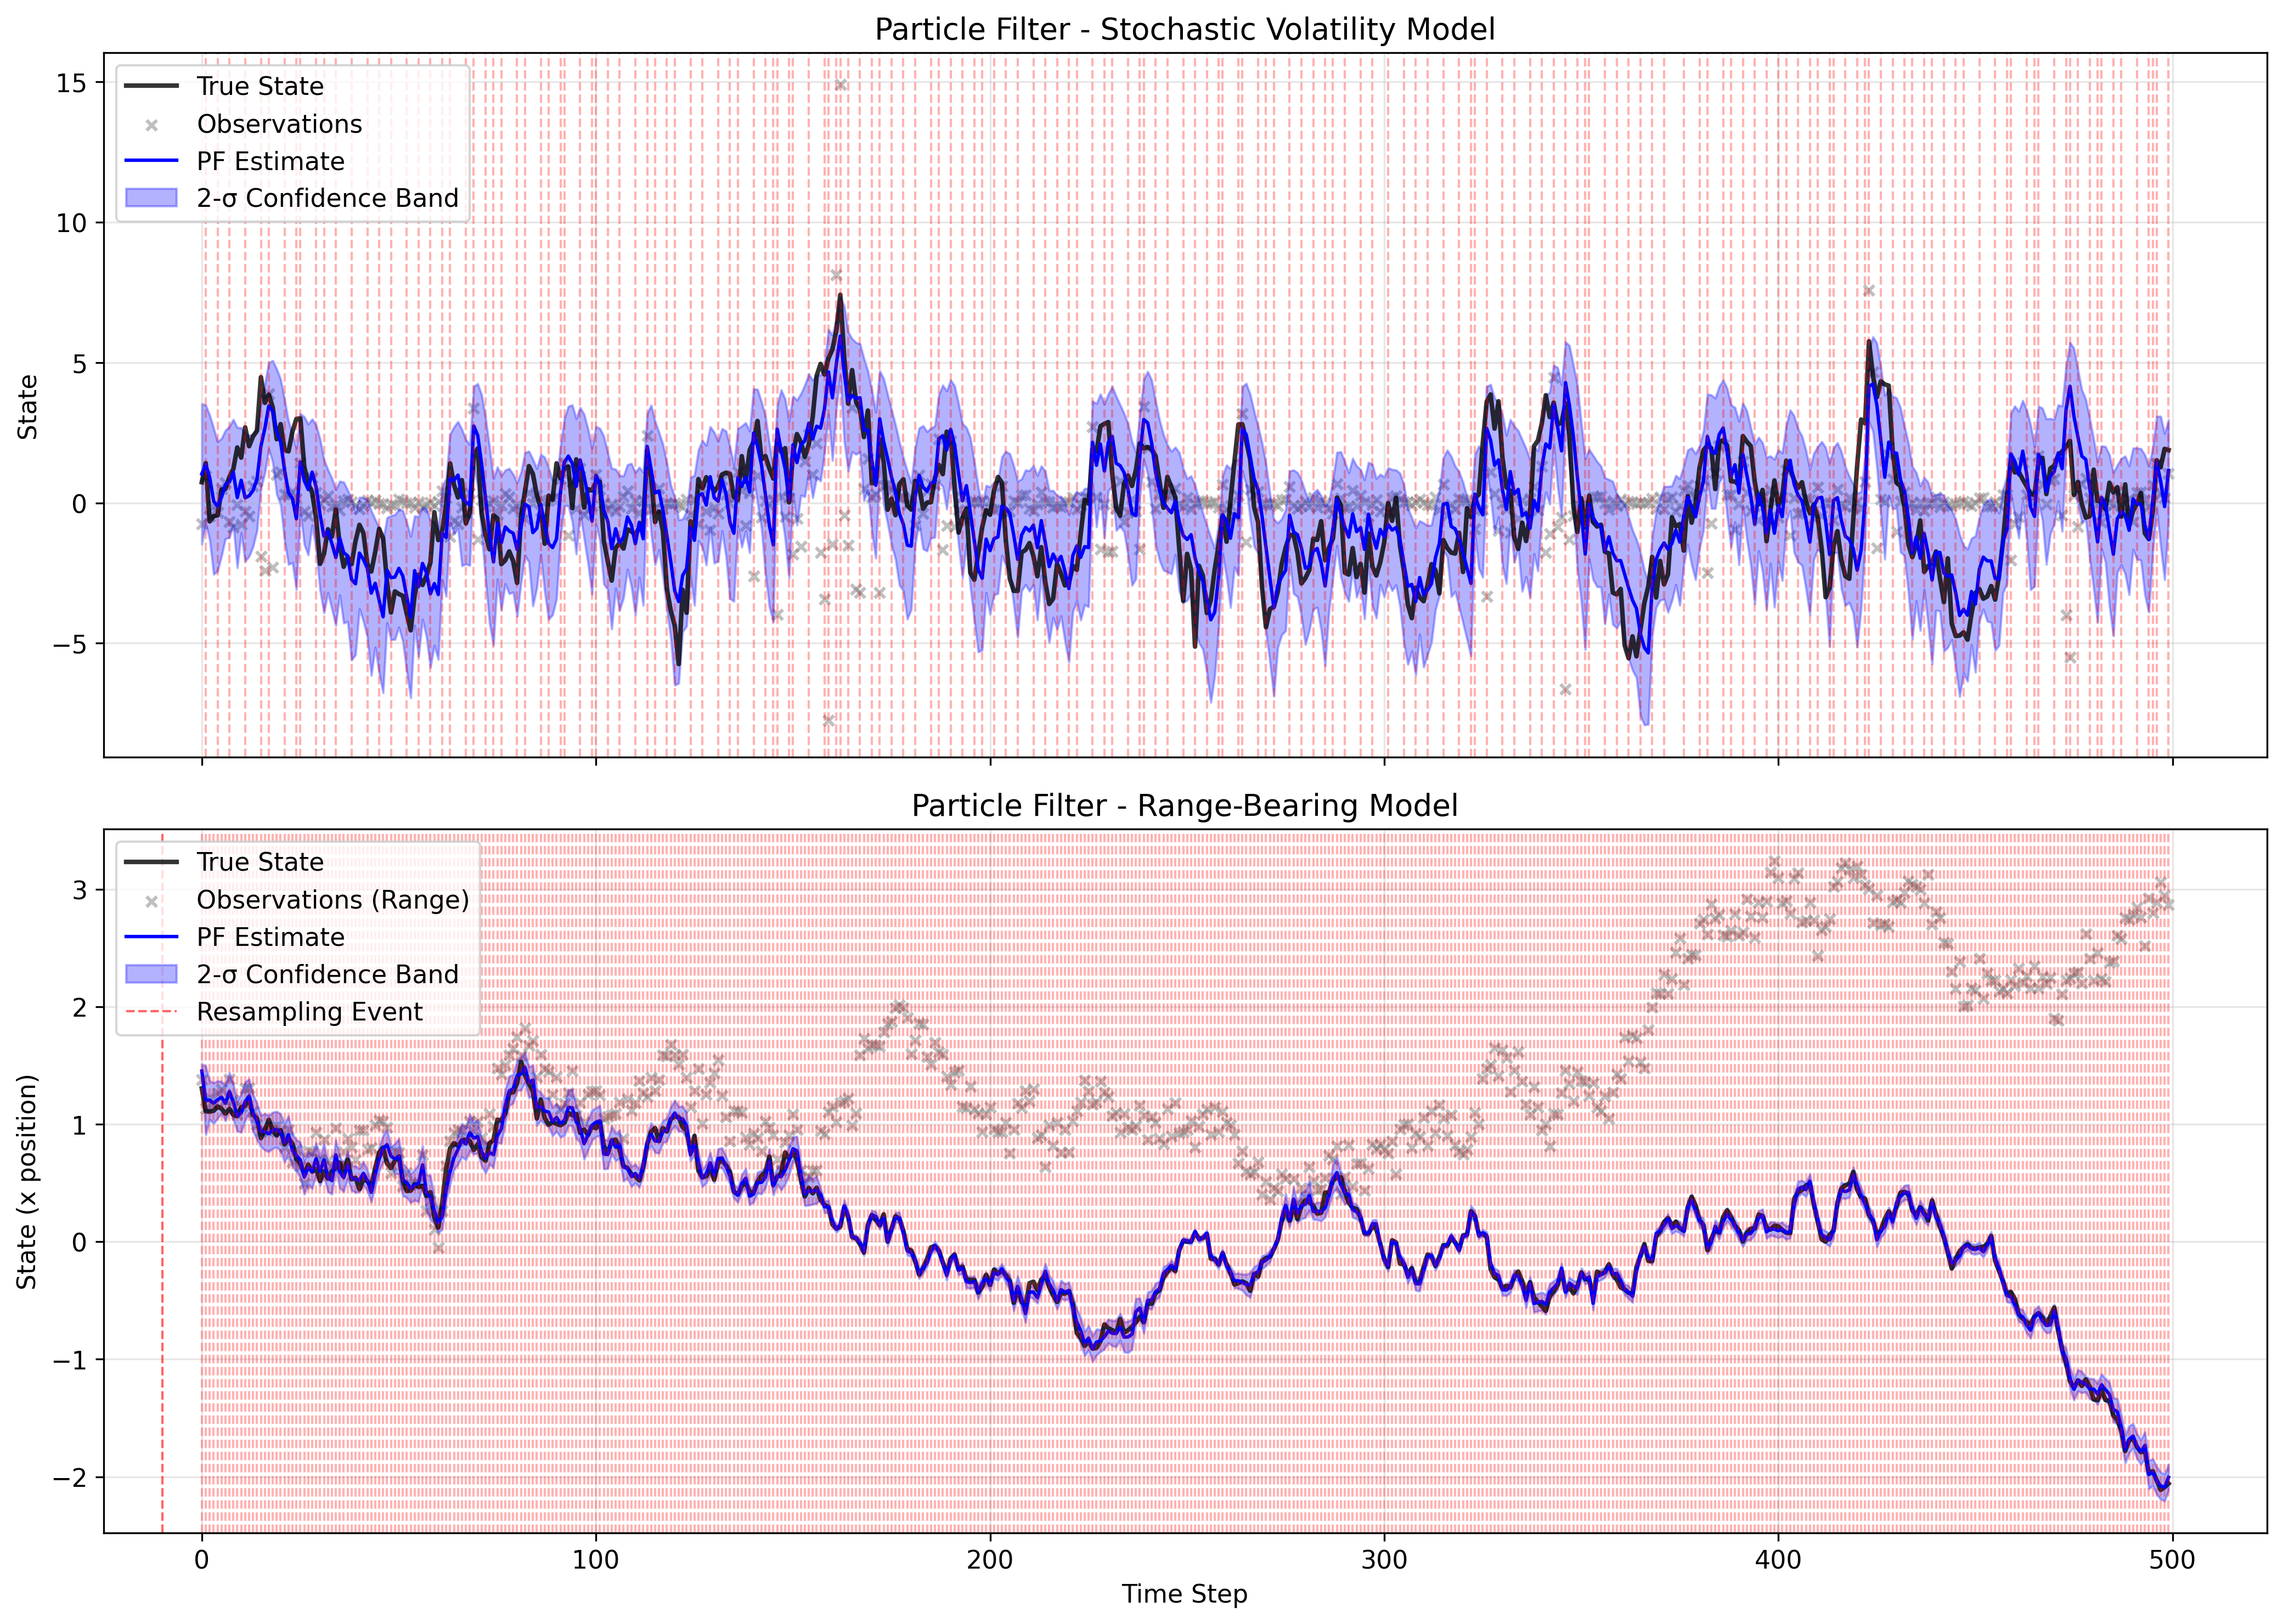
\includegraphics[width=0.8\linewidth]{particle.png}
    \caption{Bootstrap PF tracking on range-bearing and 1D stochastic volatility. The filter mean tracks the true state on both models at $N=200$.}
    \label{fig:particle_tracking}
\end{figure}

\begin{figure}[H]
    \centering
    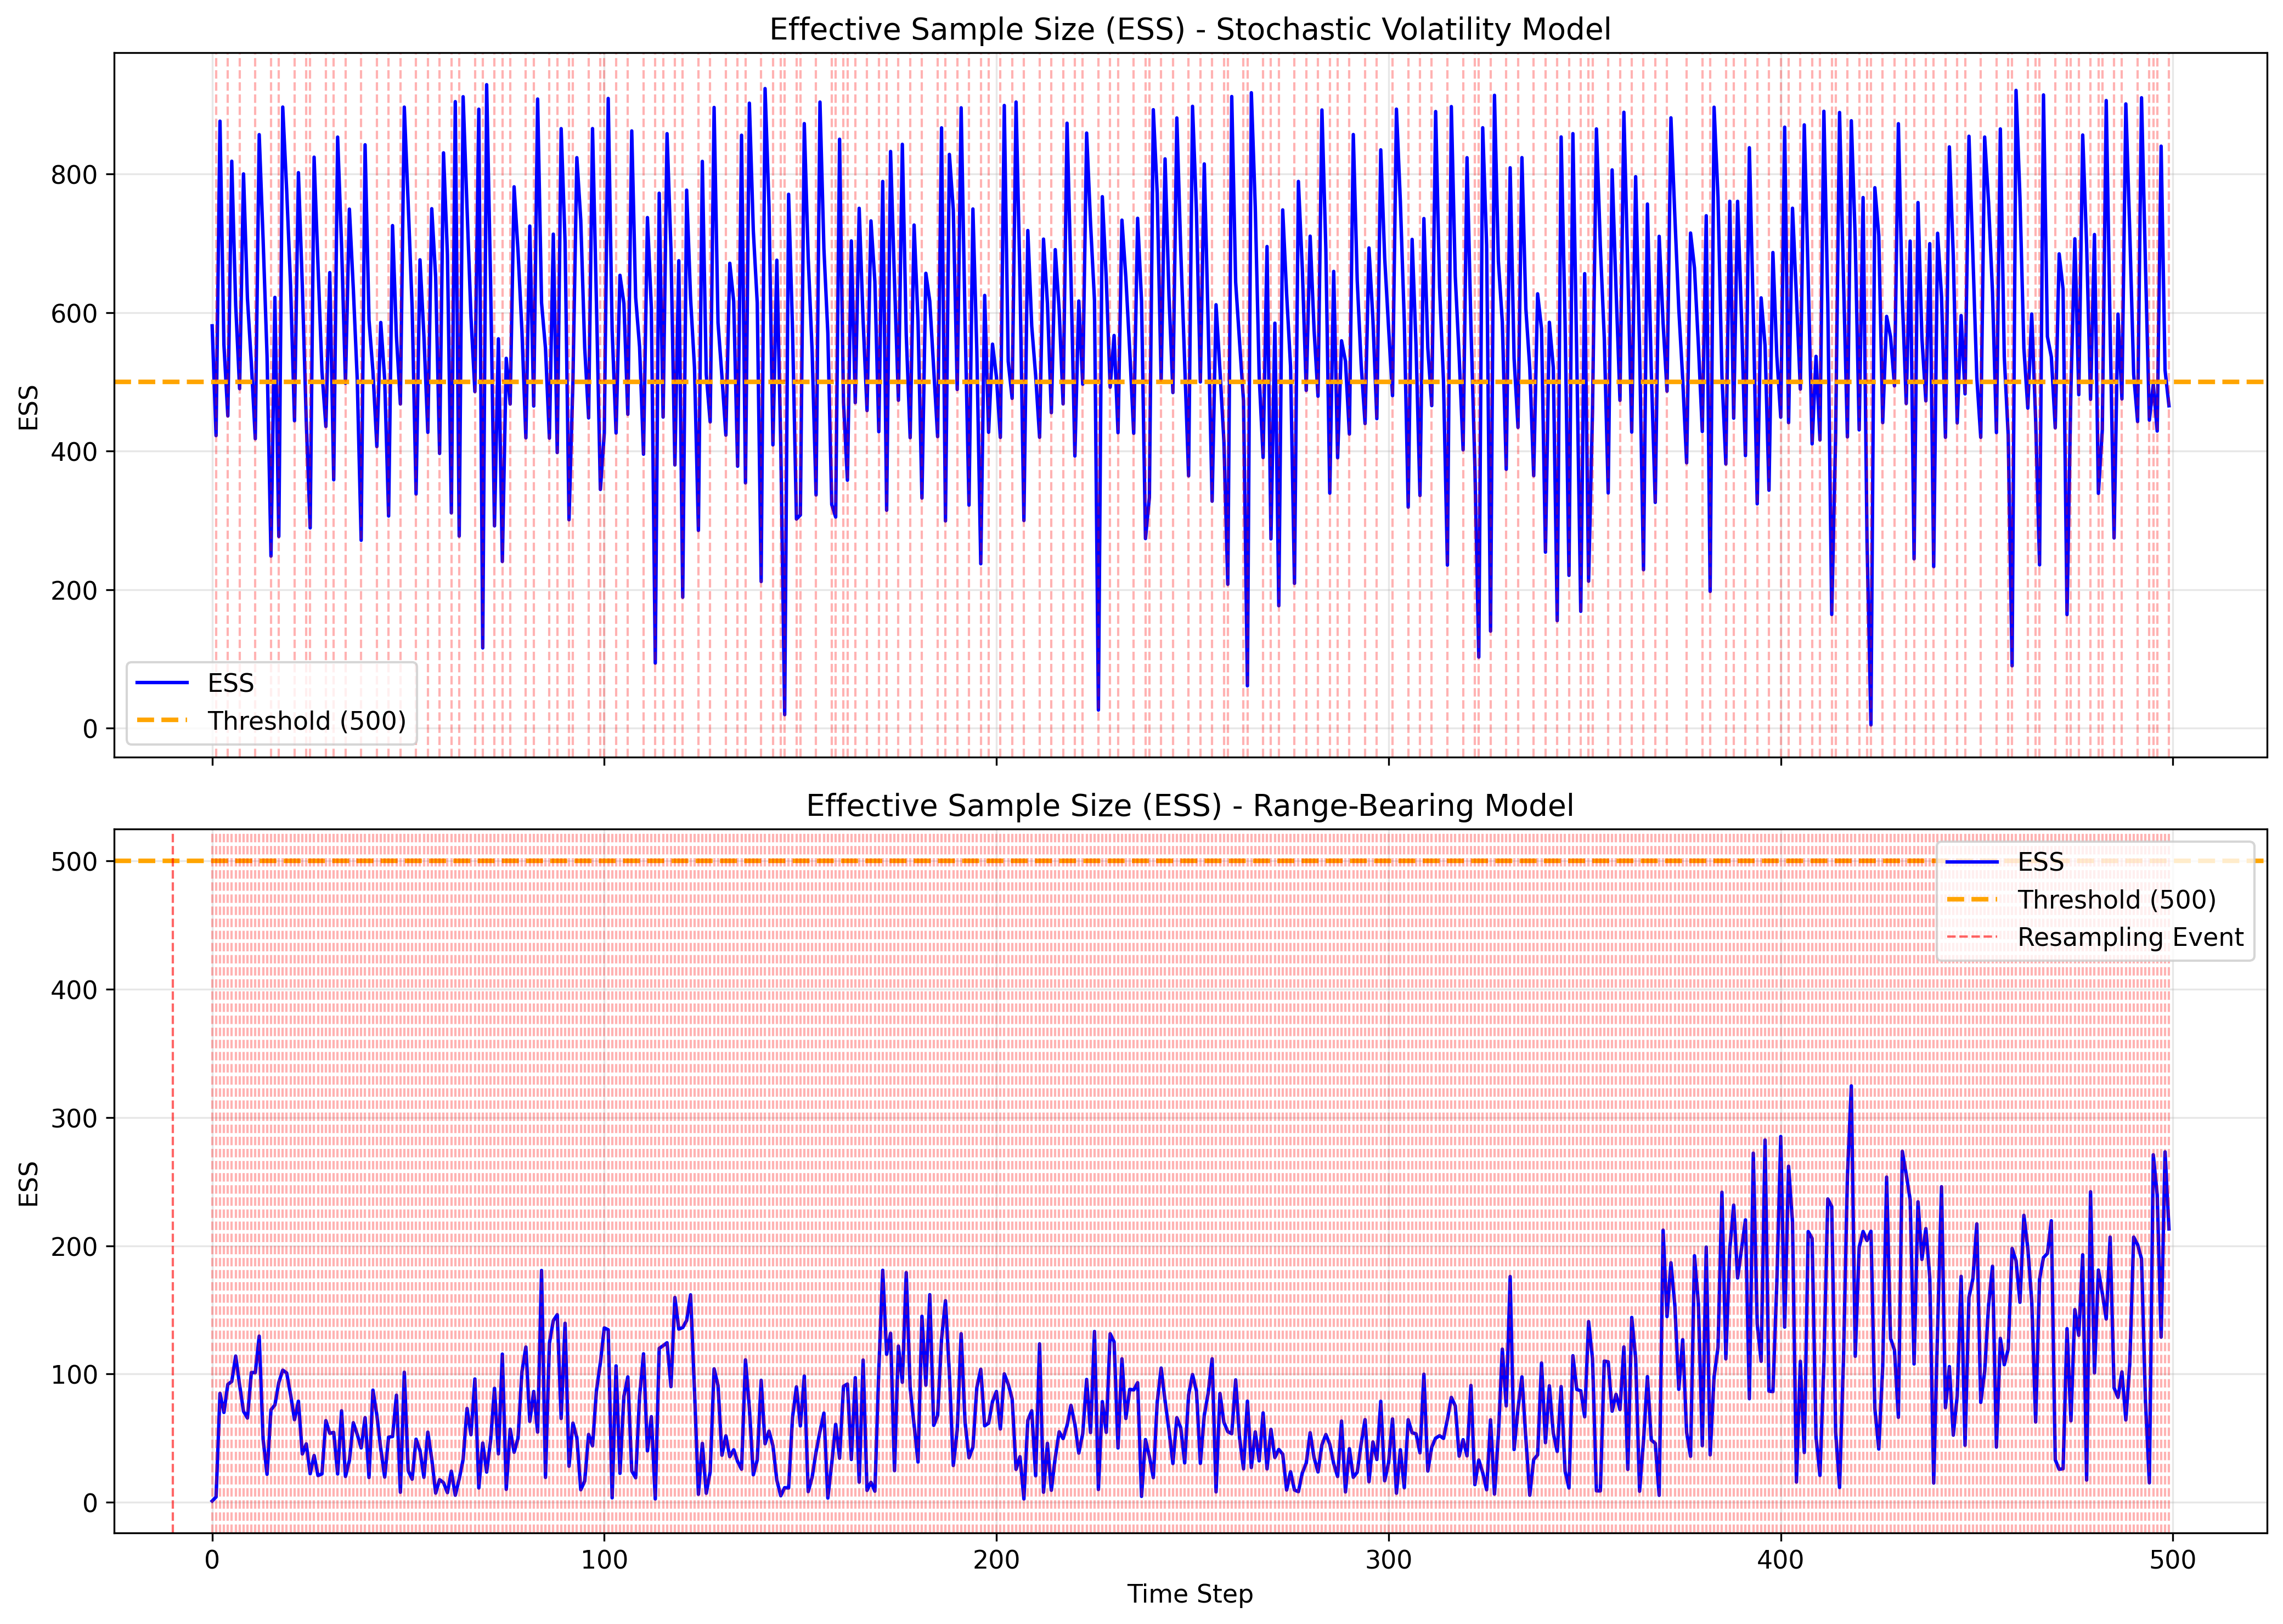
\includegraphics[width=0.8\linewidth]{particle2.png}
    \caption{Effective sample size over time for the same two runs. Range-bearing collapses within the first few steps; stochastic volatility stays above threshold longer.}
    \label{fig:ess_time}
\end{figure}

\begin{figure}[H]
    \centering
    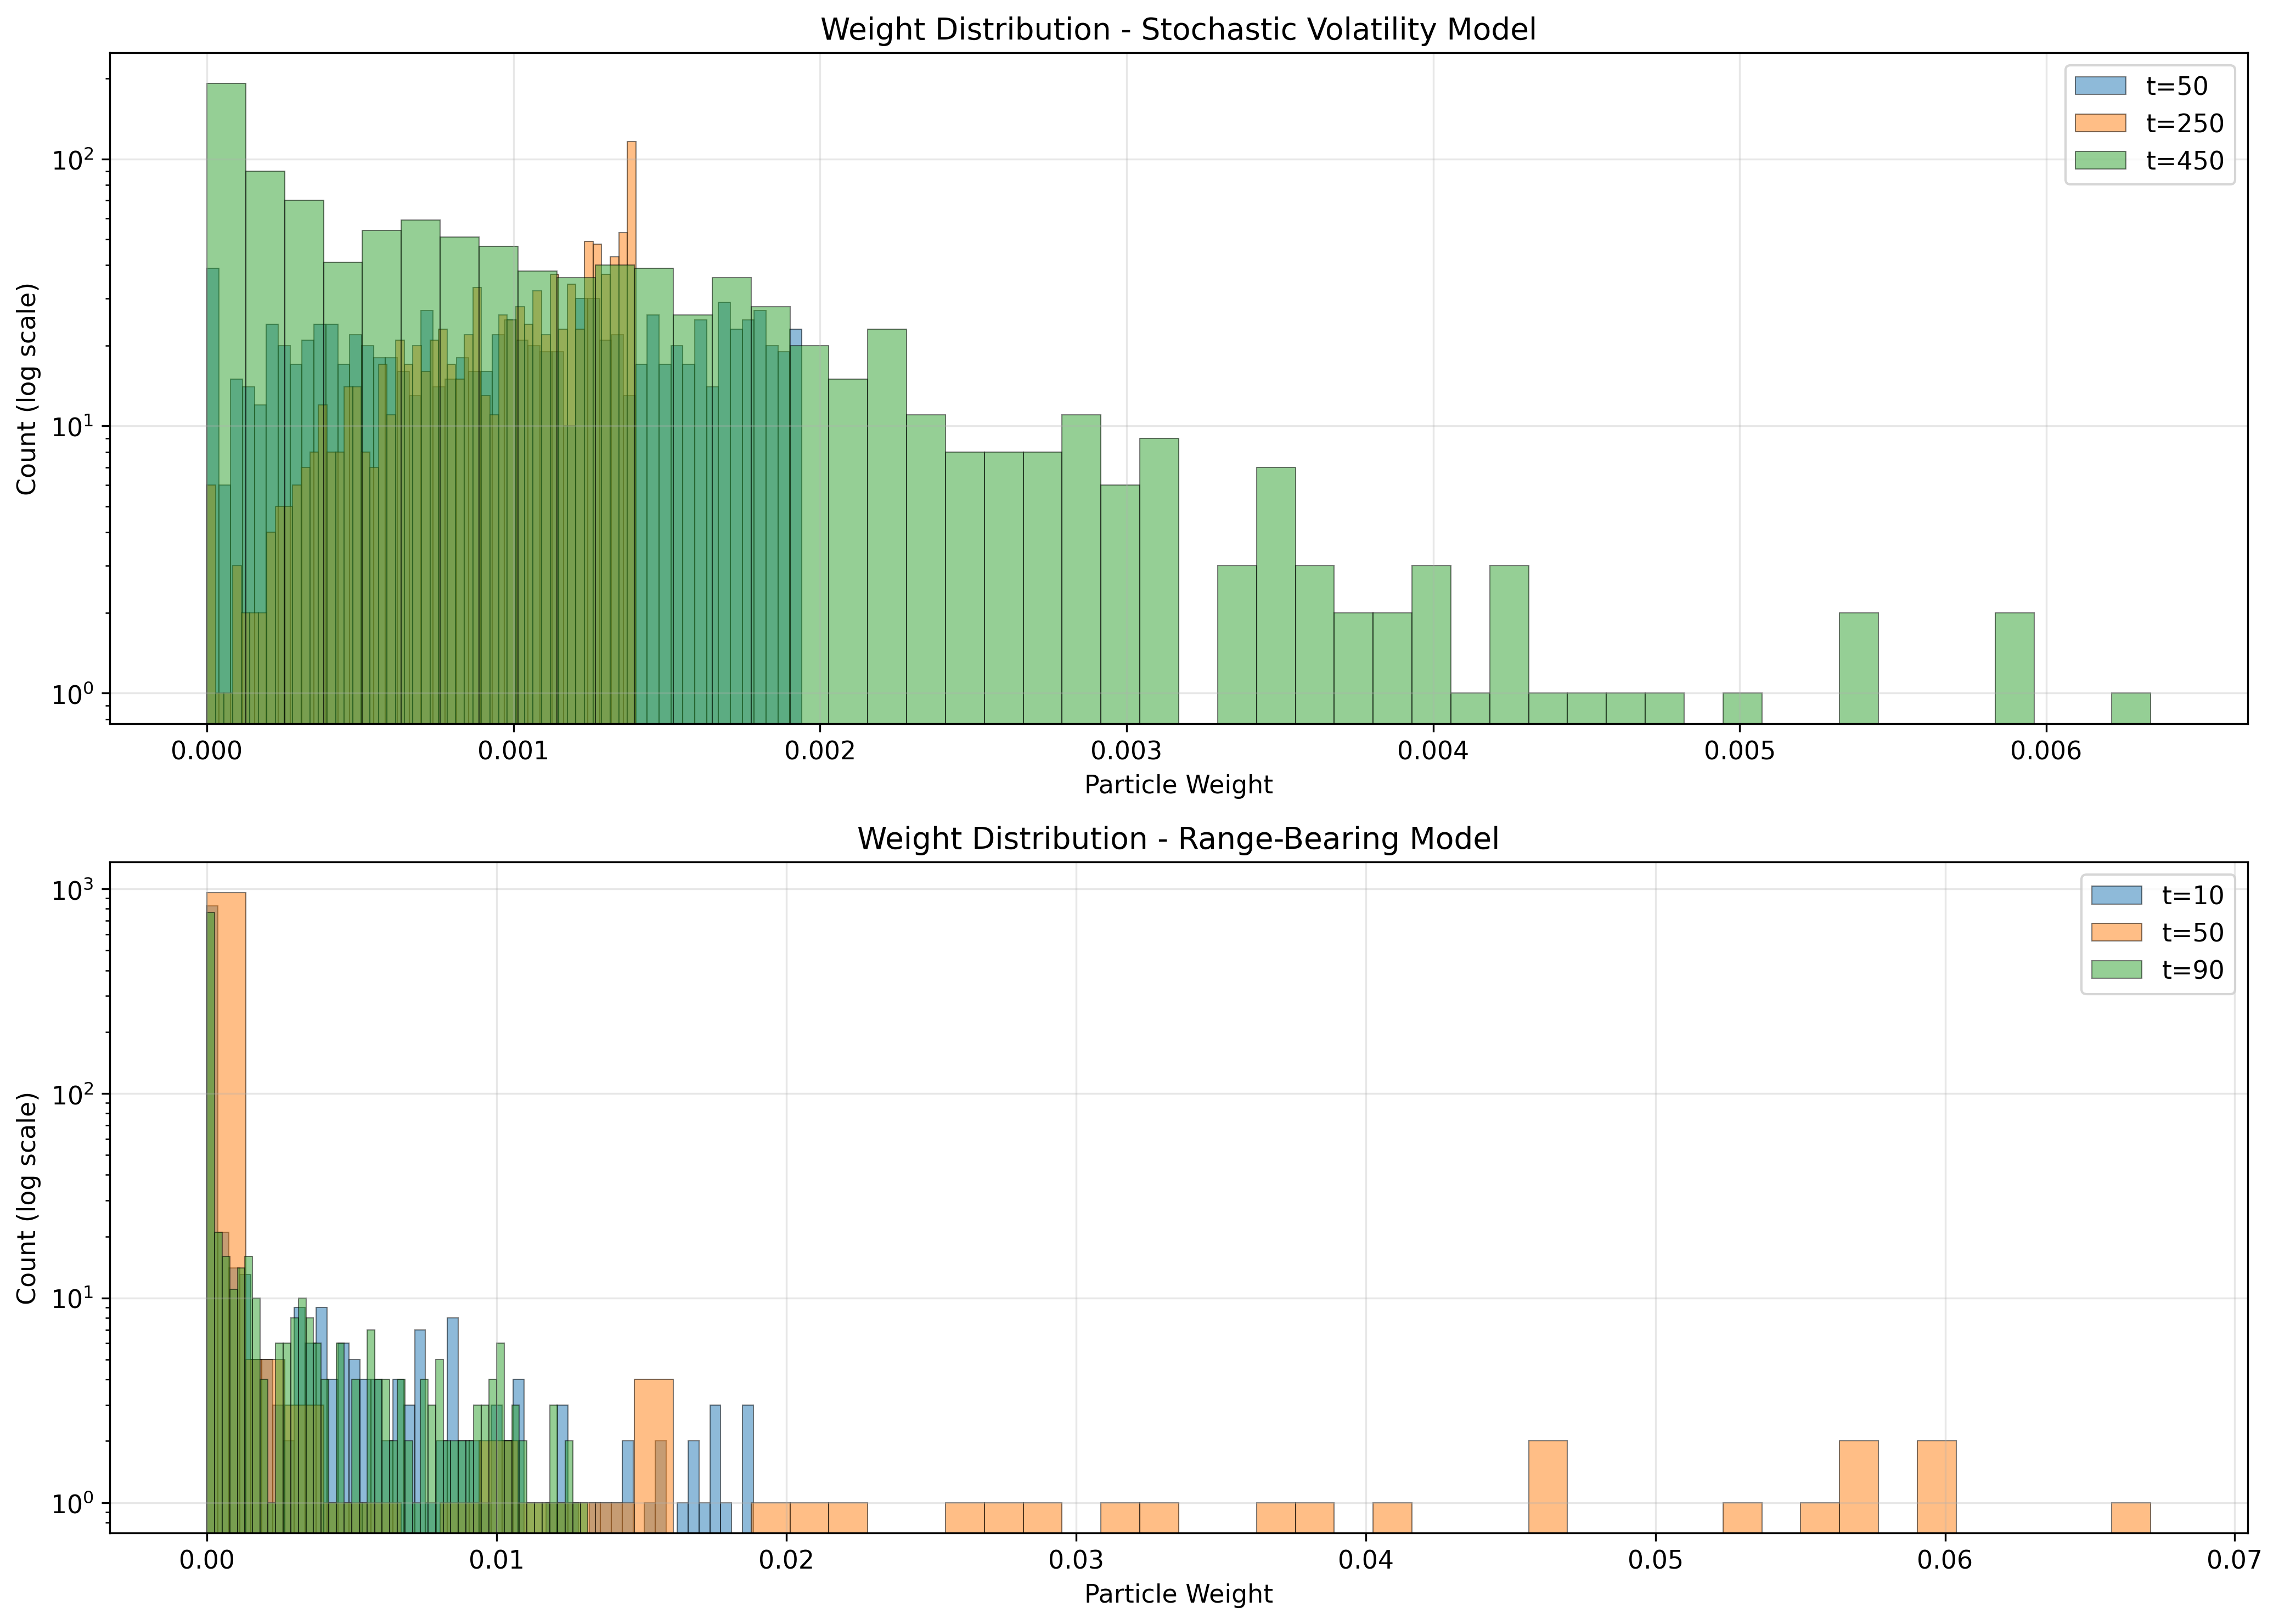
\includegraphics[width=0.8\linewidth]{particle3.png}
    \caption{Weight distribution histograms at $k=1,25,100$. The range-bearing cloud is dominated by a single particle within one step.}
    \label{fig:weight_distribution}
\end{figure}

\begin{figure}[H]
    \centering
    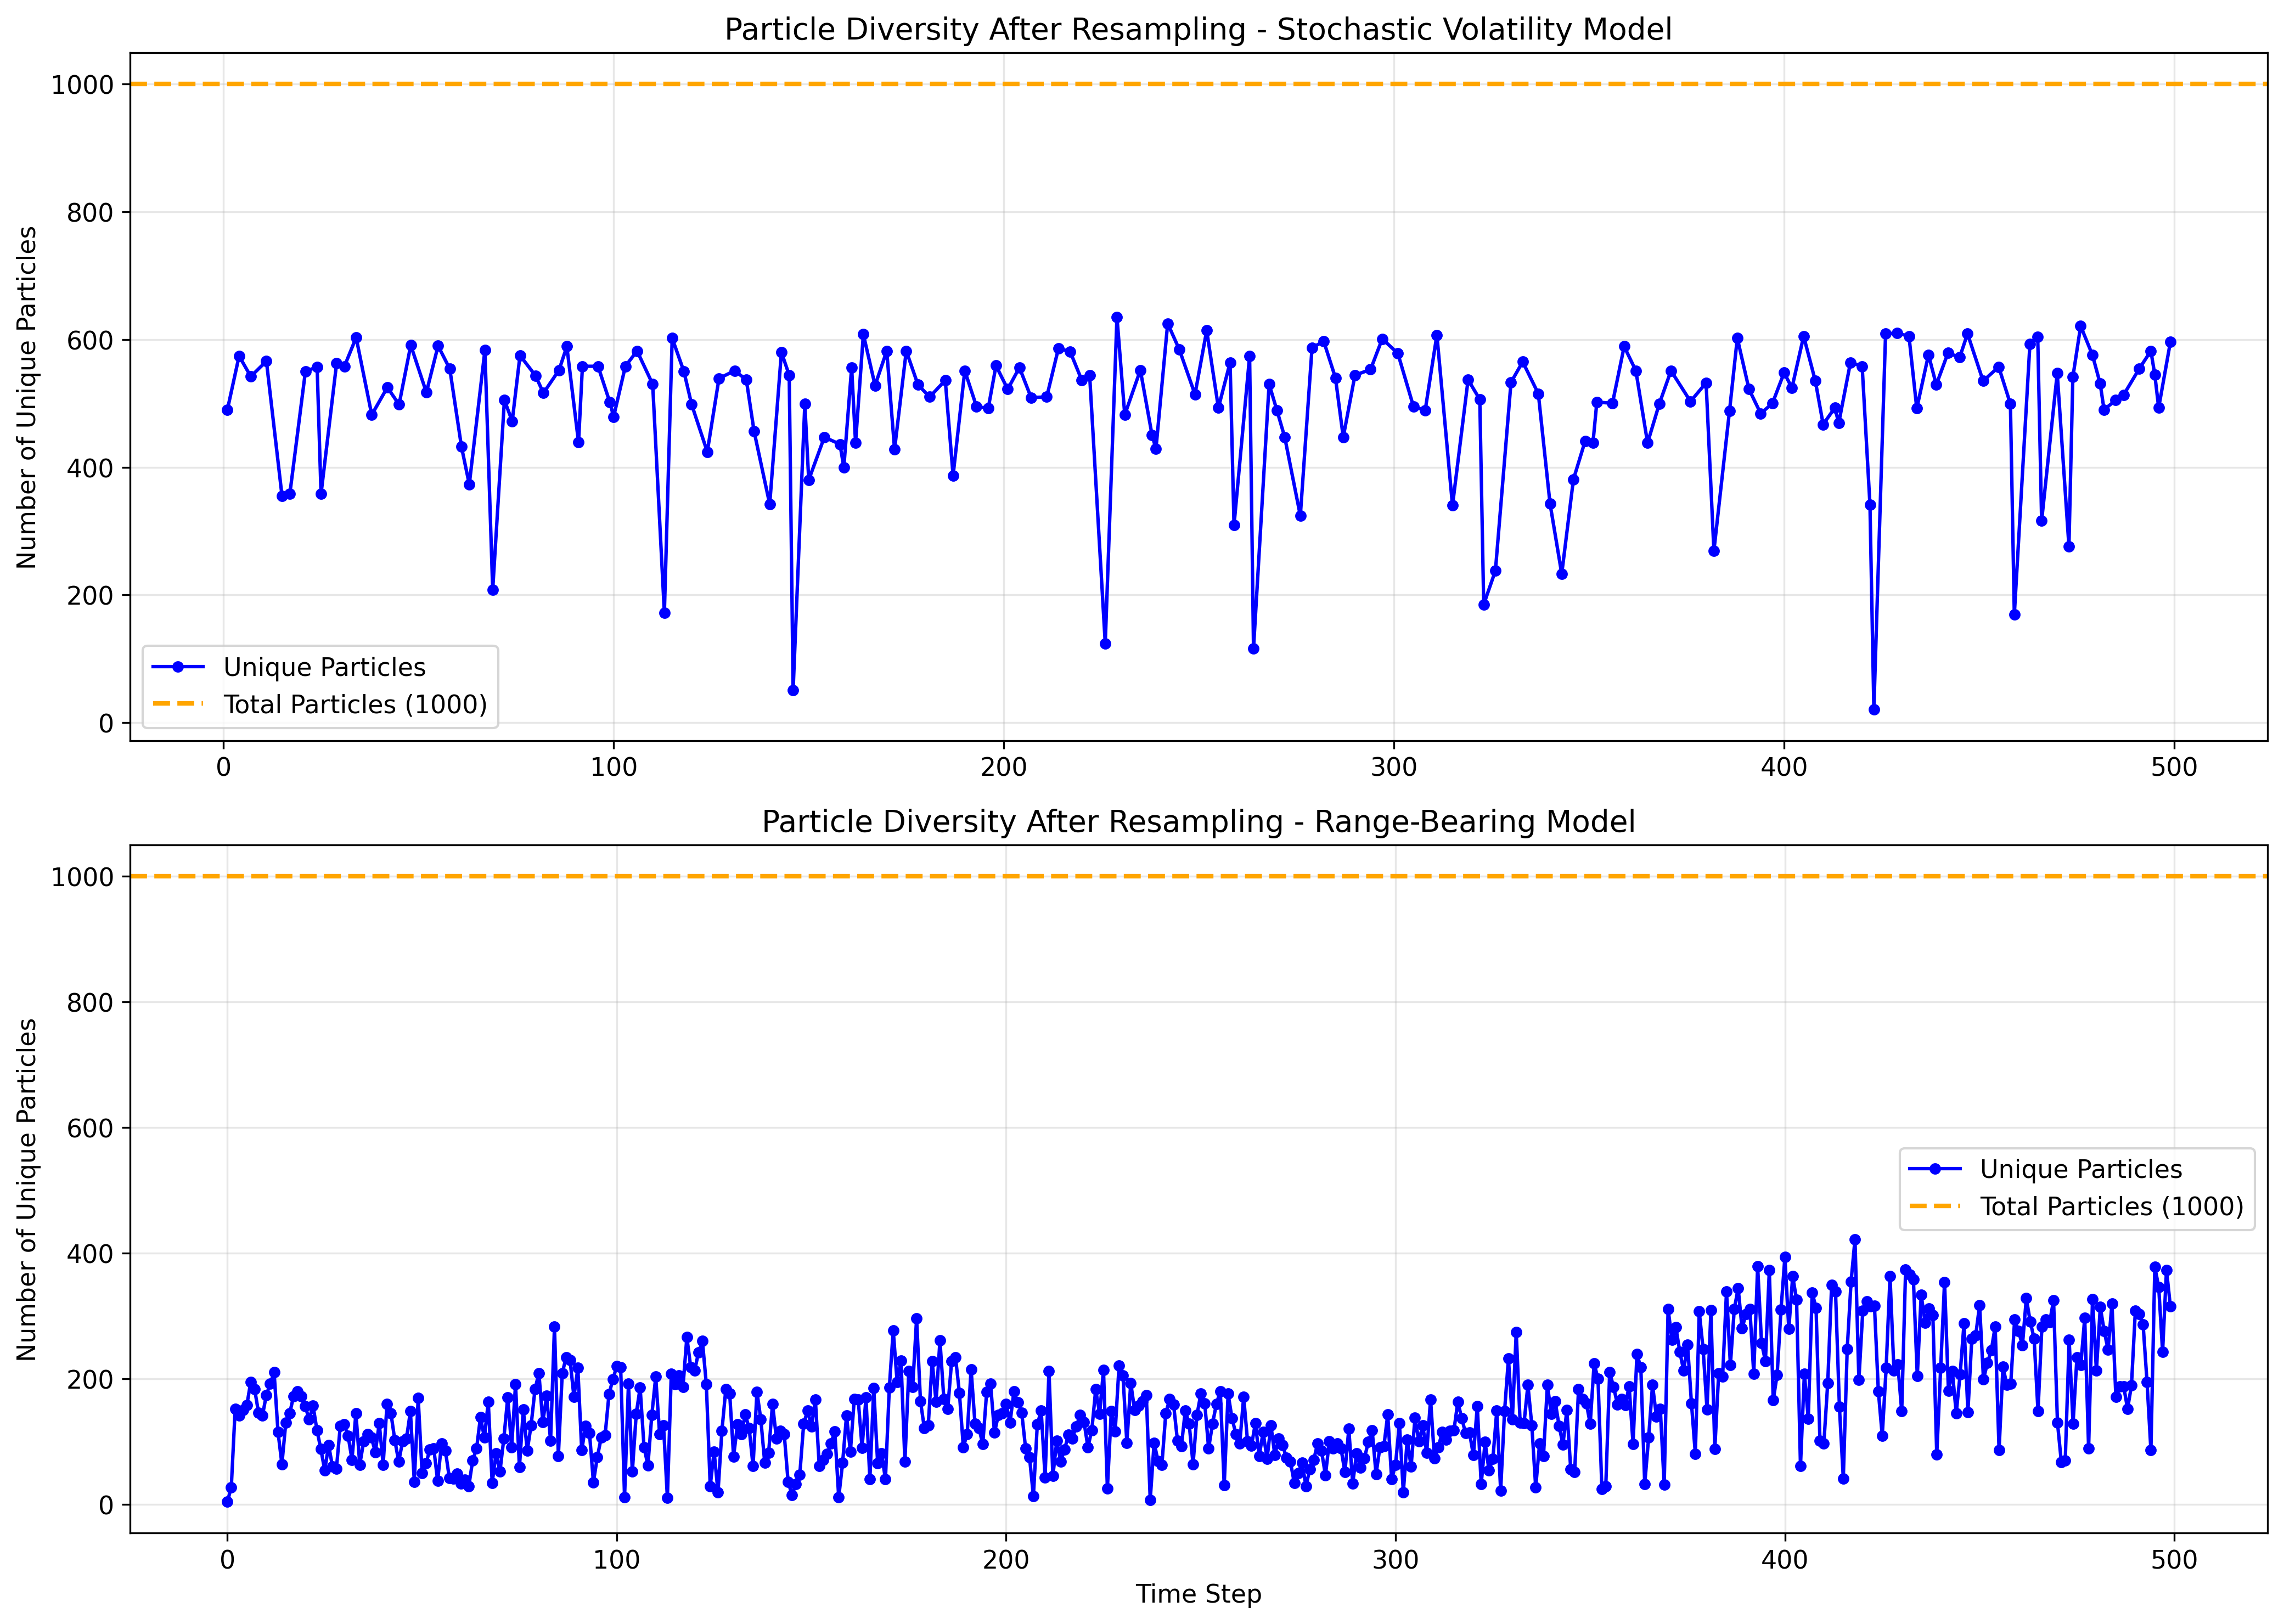
\includegraphics[width=0.8\linewidth]{particle4.png}
    \caption{Particle diversity on stochastic volatility. Diversity stays reasonable because the observation is diffuse enough to spread the weight mass.}
    \label{fig:particle_diversity}
\end{figure}

\paragraph{Empirical takeaway (§4.2).} The bootstrap PF does two useful things that EKF/UKF cannot. (i)~On the raw stochastic volatility model, where multiplicative-noise observations break every linearisation-based filter at $\mathrm{RMSE} \approx 2.04$, the bootstrap PF evaluates the likelihood directly and reaches $\mathrm{RMSE} = 1.117$ (Table~\ref{tab:edh-sv-raw}), fixing what the Kalman family could not. (ii)~On the range-bearing model, the bootstrap PF matches EKF/UKF on RMSE ($\approx 0.14$) without needing the Jacobian of $h$ at all --- useful when the measurement model is a black box. 

%(iii)~On the high-dimensional acoustic-tracking model, the bootstrap PF at a manageable $N = 200$ returns $\mathrm{RMSE} \approx 55.7$; pushing to $N = 10^6$ (with a shortened $T = 50$) reaches $\mathrm{RMSE} \approx 22.1$ but at ${\sim}160$ s wall-time per trajectory, which is not operationally useful. The ESS trajectory and weight histogram on acoustic tracking (conditional-resampling rate climbing above $0.9$ within the first few steps) are the motivation for the flow-based methods in \S4.3: they are the direct evidence that naive weight re-adjustment cannot cover high-dimensional, long-horizon targets.

\subsection{EDH/LEDH Flow Filter}
I next use Exact Daum--Huang flow and its local variants \cite{daum2010exact,daum2011particle,Li-Particle-Filtering-2017}.
\subsubsection{Use Fokker-Planck to reach the target distribution}
Start from the filtering update.
\begin{equation}
    p(x_k \mid z_{1:k}) \propto \underbrace{p(x_k \mid z_{1:k-1})}_{g(x)} \cdot \underbrace{p(z_k \mid x_k)}_{h(x)}.
\end{equation}
The Bootstrap Particle Filter handles this by reweighting: sample from $g(x)$, then multiply each particle's weight by $h(x^{(i)})$. That multiplication is precisely what causes weight degeneracy. Flow filters \cite{daum2010exact,daum2011particle} take a different route: instead of adjusting weights, move the particles. If I can find a deterministic map that transports samples from $g(x)$ into samples from $g(x)h(x)$, the update step is solved exactly---with no weights and therefore no weight degeneracy.

To do this continuously, introduce a pseudo-time $\lambda \in [0,1]$ and the \textit{log-homotopy}:
\begin{equation}
    \log p(x,\lambda) = \log g(x) + \lambda \log h(x).
\end{equation}
At $\lambda=0$, $p(x,0) = g(x)$ is the predicted distribution; at $\lambda=1$, $p(x,1) \propto g(x)h(x)$ is the posterior. I want a flow $f(x,\lambda)$ such that particles obeying
\begin{equation}
    \frac{d\v{x}}{d\lambda} = f(\v{x},\lambda)
\end{equation}
follow this homotopy path from prior to posterior.

A deterministic flow induces a density evolution governed by the zero-diffusion \textit{Fokker-Planck equation} (also called the continuity equation for probability conservation),
\begin{equation}
    \frac{\partial p}{\partial \lambda} = -\nabla \cdot (p f).
\end{equation}
The homotopy requires $\frac{\partial \log p}{\partial \lambda} = \log h(x)$, which together with the Fokker-Planck equation (dividing by $p$ and using $\nabla \cdot(pf) = p\nabla\cdot f + (\nabla p)\cdot f$) yields the fundamental constraint:
\begin{equation}
\boxed{\log h(x) = -\nabla \cdot f - (\nabla \log p) \cdot f}
\end{equation}
This is a PDE in the unknown vector field $f$, and it has infinitely many solutions. Any flow satisfying this equation will correctly transport particles from $g(x)$ to $g(x)h(x)$. The choice of $f$ is a design decision, completely analogous to the choice of proposal in weighted SMC. I just need one that is tractable to compute.

\subsubsection{Determine the evolution kernel}
\label{sec:edh_derivation}
The simplest structured choice is an \textit{affine flow}:
\begin{equation}
    f(x,\lambda) = A(\lambda)\,x + b(\lambda),
\end{equation}
where $A(\lambda)$ and $b(\lambda)$ are a matrix and vector to be determined. $A$ stretches and rotates particles while $b$ translates them. Crucially, they are not free parameters --- they must be chosen so that the flow satisfies the Fokker-Planck constraint. For an affine flow $\nabla \cdot f = \text{Tr}(A)$, and the constraint becomes algebraic once $\nabla \log p(x,\lambda)$ is known.

This is where I need an assumption. To evaluate $\nabla \log p(x,\lambda)$ in the constraint, I need to know what $p(x,\lambda)$ looks like for intermediate $\lambda$. Different assumptions lead to different flows --- different schedules for $A(\lambda)$ and $b(\lambda)$ --- but they all share the same endpoints: $\lambda = 0$ is the prior $g(x)$ and $\lambda = 1$ is the posterior $g(x)h(x)$, fixed by the homotopy construction. The assumption only determines the path taken between those two endpoints; it does not change the destination. I assume $p(x,\lambda)$ is Gaussian:
\begin{equation}
    p(x,\lambda) \sim \mathcal{N}(\bar{\eta}_\lambda, P_\lambda),
\end{equation}
with precision and mean evolving as
\begin{align}
    P_\lambda^{-1} &= P^{-1} + \lambda H^T R^{-1} H, \\
    \bar{\eta}_\lambda &= P_\lambda\bigl[P^{-1}\bar{\eta}_0 + \lambda H^T R^{-1} z\bigr].
\end{align}
This is the only role of the Gaussian assumption: it gives a tractable expression for $\nabla \log p(x,\lambda) = -P_\lambda^{-1}(x - \bar{\eta}_\lambda)$, which is substituted into the constraint to solve for $A$ and $b$. A different assumption about the intermediate distribution would yield a different flow schedule, but the particles would still travel between the same prior and posterior.

With the Gaussian form, $\nabla \log p(x,\lambda) = -P_\lambda^{-1}(x - \bar{\eta}_\lambda)$. Differentiating the precision with respect to $\lambda$ and using the matrix identity $dP_\lambda/d\lambda = -P_\lambda(dP_\lambda^{-1}/d\lambda)P_\lambda$ gives
\begin{equation}
    \frac{dP_\lambda}{d\lambda} = -P_\lambda H^T R^{-1} H P_\lambda.
\end{equation}
Matching this with the covariance evolution under the affine flow, $AP_\lambda + P_\lambda A^T = dP_\lambda/d\lambda$, and solving the resulting Riccati equation yields:
\begin{equation}
\boxed{A(\lambda) = -\frac{1}{2} P_\lambda H^T R^{-1} H = -\frac{1}{2} P H^T (\lambda H P H^T + R)^{-1} H}
\end{equation}
For $b(\lambda)$, requiring that the mean evolves correctly under the flow gives:
\begin{equation}
\boxed{b(\lambda) = (I + 2\lambda A)\bigl[(I + \lambda A) P H^T R^{-1} z + A \bar{\eta}_0\bigr]}
\end{equation}
These two equations define the EDH flow completely. The log-homotopy definition forces $\lambda$ to run from $0$ to $1$, so the particle integration over $\lambda$ is a finite integral solved numerically with small steps $\varepsilon_j$.

%\paragraph{Why the result is not Gaussian.}
%Once $A(\lambda)$ and $b(\lambda)$ are derived, discard the Gaussian assumption entirely. The particles are just points in state space being pushed by the ODE $dx^{(i)}/d\lambda = A(\lambda)x^{(i)} + b(\lambda)$. Nothing in this ODE forces the output cloud to be Gaussian --- the Gaussian assumption determined how the wind was computed, not where the particles end up.

%Think of $A(\lambda)$ and $b(\lambda)$ as a spatially uniform wind field: every particle feels the same push regardless of where it sits. If the prior is exactly Gaussian and the model is truly linear Gaussian, this wind is exact and the particles arrive at a perfect Gaussian posterior. But if the prior is non-Gaussian, or $h(x)$ is nonlinear so that $H$ is only an approximation, the wind is only approximately correct. Some particles get pushed too far, others not far enough. The resulting cloud can have any shape: heavy tails, skew, multi-modality. The Gaussian assumption shaped the wind field; it does not shape the output.

\subsubsection{EDH vs.\ LEDH: incremental improvements in linearization quality.}
All variants use exactly the same framework: the same log-homotopy, the same affine ansatz, the same Gaussian assumption for $\nabla \log p$. They differ only in \textit{where and when} the Jacobian $H = \partial h / \partial x$ is evaluated. There are three levels of refinement:

\begin{itemize}
    \item \textbf{EDH (fixed global linearization):} $H$ is computed once at the global predicted mean $\bar{\eta}_0$ at the start of the flow ($\lambda = 0$) and held fixed for the entire $\lambda$ integration. All particles share the same $A(\lambda)$ and $b(\lambda)$ at every step. This is the most efficient variant but the least accurate: as particles move during the flow, the mean $\bar{\eta}(\lambda)$ drifts away from $\bar{\eta}_0$, yet the linearization never corrects for this.

    \item \textbf{EDH (intermediate re-linearization):} At each $\lambda$ step, $H$ is re-evaluated at the current global mean $\bar{\eta}^{(\lambda)}$, and the nonlinear correction $e = h(\bar{\eta}^{(\lambda)}) - H\bar{\eta}^{(\lambda)}$ is computed. The drift vector $b$ is updated to use $(z - e)$ instead of $z$, capturing the residual between the true observation function and its local linearization. The wind field is still uniform across particles — all particles share the same $A$ and $b$ at each step — but both are recomputed at each step to track where the cloud has moved. This is strictly richer than the fixed variant: not only does $H$ improve, but $b$ also corrects for the nonlinearity of $h$ at the current operating point.

    \item \textbf{LEDH (local, per-particle linearization)} \cite{Li-Particle-Filtering-2017}\textbf{:} $H^{(i)} = \partial h/\partial x\big|_{x^{(i)}(\lambda)}$ is computed at each particle's own current position at each $\lambda$ step, giving every particle its own $A^{(i)}(\lambda)$ and $b^{(i)}(\lambda)$. Each particle gets its own local affine drift. The linearization error is controlled by the distance from $x^{(i)}$ to the linearization point—which is now zero. This is the most accurate variant, at the cost of $N$ Jacobian evaluations per $\lambda$ step.
\end{itemize}

Each step in this hierarchy adds one more correction to where the linearization is taken—across particles, across pseudo-time, or both. None of them is a different algorithm. They are the same affine flow with progressively better approximations to $\nabla \log p$ plugged in.

\subsubsection{Algorithm}

All three variants share the same structural role for the global EKF/UKF: it runs in parallel with the particle cloud \textit{solely} to supply the covariance $\mathbf{P}$ and the linearization point needed to compute the flow kernel $A(\lambda), b(\lambda)$. It is never used to produce filter estimates. The reported output—the posterior mean $m_k$ and covariance $P_k$—is always taken from the empirical particle ensemble:
\begin{equation}
    m_k = \frac{1}{N}\sum_i \boldsymbol{\eta}^{(i)}, \qquad P_k = \frac{1}{N}\sum_i (\boldsymbol{\eta}^{(i)} - m_k)(\boldsymbol{\eta}^{(i)} - m_k)^\top.
\end{equation}
To keep the global filter from drifting away from the particle cloud, a \textit{feedback step} resets the EKF/UKF mean to the current empirical mean at the start of each time step before prediction. The EKF/UKF covariance $\mathbf{P}$ is then used as the kernel covariance, but the covariance estimate reported to the user is the empirical one above. The algorithm below is the version I use.

\begin{algorithm}[H]
\caption{EDH Flow Filter (Fixed Global Linearization)}
\label{alg:edh_fixed}
\begin{algorithmic}[1]
\REQUIRE Particles $\{\boldsymbol{\eta}^{(i)}\}_{i=1}^N$, global EKF/UKF state $(\bar{\boldsymbol{\eta}}, \mathbf{P})$
\REQUIRE Lambda schedule $\{\varepsilon_j\}_{j=1}^{n_\lambda}$
\FOR{$k = 1, 2, \ldots, T$}
  \STATE \textbf{Feedback:} $\bar{\boldsymbol{\eta}} \leftarrow \frac{1}{N}\sum_i \boldsymbol{\eta}^{(i)}$ \hfill (reset global mean to empirical mean)
  \STATE \textbf{Predict (EKF/UKF):} $(\bar{\boldsymbol{\eta}}_0, \mathbf{P}) \leftarrow \text{EKF/UKF predict}(\bar{\boldsymbol{\eta}}, \mathbf{P})$
  \STATE \textbf{Predict (particles):} $\boldsymbol{\eta}^{(i)} \sim p(\mathbf{x}_k \mid \boldsymbol{\eta}^{(i)})$ for $i=1,\ldots,N$
  \STATE $\mathbf{H} \leftarrow \frac{\partial \mathbf{h}}{\partial \mathbf{x}}\Big|_{\bar{\boldsymbol{\eta}}_0}$ \hfill (\textbf{fixed}: linearize once at $\bar{\boldsymbol{\eta}}_0$, held for all $\lambda$ steps)
  \STATE $\lambda \leftarrow 0$
  \FOR{$j = 1, 2, \ldots, n_\lambda$}
    \STATE $\lambda \leftarrow \lambda + \varepsilon_j$
    \STATE $\mathbf{A} \leftarrow -\tfrac{1}{2}\mathbf{P}\mathbf{H}^\top(\lambda\mathbf{H}\mathbf{P}\mathbf{H}^\top + \mathbf{R})^{-1}\mathbf{H}$
    \STATE $\mathbf{b} \leftarrow (\mathbf{I}+2\lambda\mathbf{A})[(\mathbf{I}+\lambda\mathbf{A})\mathbf{P}\mathbf{H}^\top\mathbf{R}^{-1}\mathbf{z}_k + \mathbf{A}\bar{\boldsymbol{\eta}}_0]$
    \STATE $\boldsymbol{\eta}^{(i)} \leftarrow \boldsymbol{\eta}^{(i)} + \varepsilon_j(\mathbf{A}\boldsymbol{\eta}^{(i)} + \mathbf{b})$ for all $i$
  \ENDFOR
  \STATE \textbf{Update (EKF/UKF):} $(\bar{\boldsymbol{\eta}}, \mathbf{P}) \leftarrow \text{EKF/UKF update}(\bar{\boldsymbol{\eta}}_0, \mathbf{P}, \mathbf{z}_k)$ \hfill (kernel only; not reported)
  \STATE \textbf{Output:} $m_k = \frac{1}{N}\sum_i \boldsymbol{\eta}^{(i)}$, \; $P_k = \frac{1}{N}\sum_i(\boldsymbol{\eta}^{(i)}-m_k)(\boldsymbol{\eta}^{(i)}-m_k)^\top$
\ENDFOR
\end{algorithmic}
\end{algorithm}

\begin{algorithm}[H]
\caption{EDH Flow Filter (Intermediate Re-linearization)}
\label{alg:edh_relinear}
\begin{algorithmic}[1]
\REQUIRE Same setup as Algorithm~\ref{alg:edh_fixed}
\FOR{$k = 1, 2, \ldots, T$}
  \STATE \textbf{Feedback, Predict (EKF/UKF), Predict (particles):} same as Algorithm~\ref{alg:edh_fixed}
  \STATE $\bar{\boldsymbol{\eta}}^{(\lambda)} \leftarrow \bar{\boldsymbol{\eta}}_0$ \hfill (track current global mean through flow)
  \STATE $\lambda \leftarrow 0$
  \FOR{$j = 1, 2, \ldots, n_\lambda$}
    \STATE $\lambda \leftarrow \lambda + \varepsilon_j$
    \STATE $\mathbf{H} \leftarrow \frac{\partial \mathbf{h}}{\partial \mathbf{x}}\Big|_{\bar{\boldsymbol{\eta}}^{(\lambda)}}$ \hfill (\textbf{re-linearize} at current global mean $\bar{\boldsymbol{\eta}}^{(\lambda)}$)
    \STATE $\mathbf{e} \leftarrow \mathbf{h}(\bar{\boldsymbol{\eta}}^{(\lambda)}) - \mathbf{H}\bar{\boldsymbol{\eta}}^{(\lambda)}$ \hfill (nonlinear correction at current mean)
    \STATE $\mathbf{A} \leftarrow -\tfrac{1}{2}\mathbf{P}\mathbf{H}^\top(\lambda\mathbf{H}\mathbf{P}\mathbf{H}^\top + \mathbf{R})^{-1}\mathbf{H}$
    \STATE $\mathbf{b} \leftarrow (\mathbf{I}+2\lambda\mathbf{A})[(\mathbf{I}+\lambda\mathbf{A})\mathbf{P}\mathbf{H}^\top\mathbf{R}^{-1}(\mathbf{z}_k - \mathbf{e}) + \mathbf{A}\bar{\boldsymbol{\eta}}_0]$
    \STATE $\bar{\boldsymbol{\eta}}^{(\lambda)} \leftarrow \bar{\boldsymbol{\eta}}^{(\lambda)} + \varepsilon_j(\mathbf{A}\bar{\boldsymbol{\eta}}^{(\lambda)} + \mathbf{b})$ \hfill (advance mean for next re-linearization)
    \STATE $\boldsymbol{\eta}^{(i)} \leftarrow \boldsymbol{\eta}^{(i)} + \varepsilon_j(\mathbf{A}\boldsymbol{\eta}^{(i)} + \mathbf{b})$ for all $i$
  \ENDFOR
  \STATE \textbf{Update (EKF/UKF):} same as Algorithm~\ref{alg:edh_fixed} \hfill (kernel only; not reported)
  \STATE \textbf{Output:} $m_k = \frac{1}{N}\sum_i \boldsymbol{\eta}^{(i)}$, \; $P_k = \frac{1}{N}\sum_i(\boldsymbol{\eta}^{(i)}-m_k)(\boldsymbol{\eta}^{(i)}-m_k)^\top$
\ENDFOR
\end{algorithmic}
\end{algorithm}

\begin{algorithm}[H]
\caption{LEDH Flow Filter (Local Per-Particle Linearization)}
\label{alg:ledh}
\begin{algorithmic}[1]
\REQUIRE Same setup as Algorithm~\ref{alg:edh_fixed}
\FOR{$k = 1, 2, \ldots, T$}
  \STATE \textbf{Feedback, Predict (EKF/UKF), Predict (particles):} same as Algorithm~\ref{alg:edh_fixed}
  \STATE $\lambda \leftarrow 0$
  \FOR{$j = 1, 2, \ldots, n_\lambda$}
    \STATE $\lambda \leftarrow \lambda + \varepsilon_j$
    \FOR{each particle $i$ (batched)}
      \STATE $\mathbf{H}^{(i)} \leftarrow \frac{\partial \mathbf{h}}{\partial \mathbf{x}}\Big|_{\boldsymbol{\eta}^{(i)}}$ \hfill (\textbf{re-linearize} at each particle's own position)
      \STATE $\mathbf{e}^{(i)} \leftarrow \mathbf{h}(\boldsymbol{\eta}^{(i)}) - \mathbf{H}^{(i)}\boldsymbol{\eta}^{(i)}$ \hfill (nonlinear offset correction)
      \STATE $\mathbf{A}^{(i)} \leftarrow -\tfrac{1}{2}\mathbf{P}\mathbf{H}^{(i)\top}(\lambda\mathbf{H}^{(i)}\mathbf{P}\mathbf{H}^{(i)\top} + \mathbf{R})^{-1}\mathbf{H}^{(i)}$
      \STATE $\mathbf{b}^{(i)} \leftarrow (\mathbf{I}+2\lambda\mathbf{A}^{(i)})[(\mathbf{I}+\lambda\mathbf{A}^{(i)})\mathbf{P}\mathbf{H}^{(i)\top}\mathbf{R}^{-1}(\mathbf{z}_k - \mathbf{e}^{(i)}) + \mathbf{A}^{(i)}\bar{\boldsymbol{\eta}}_0]$
      \STATE $\boldsymbol{\eta}^{(i)} \leftarrow \boldsymbol{\eta}^{(i)} + \varepsilon_j(\mathbf{A}^{(i)}\boldsymbol{\eta}^{(i)} + \mathbf{b}^{(i)})$
    \ENDFOR
  \ENDFOR
  \STATE \textbf{Update (EKF/UKF):} same as Algorithm~\ref{alg:edh_fixed} \hfill (kernel only; not reported)
  \STATE \textbf{Output:} $m_k = \frac{1}{N}\sum_i \boldsymbol{\eta}^{(i)}$, \; $P_k = \frac{1}{N}\sum_i(\boldsymbol{\eta}^{(i)}-m_k)(\boldsymbol{\eta}^{(i)}-m_k)^\top$
\ENDFOR
\end{algorithmic}
\end{algorithm}

%\subsubsection{Experiments}
%Table~\ref{tab:range_bearing_comparison} compares all five filters on the range-bearing model. The LEDH invertible filter achieves the best RMSE while the bootstrap PF requires the most particles. Table~\ref{tab:acoustic_tracking_comparison} shows results on the acoustic tracking model (4 targets, 25 sensors), a higher-dimensional problem where the global EDH filters struggle due to the linearisation approximation. The LEDH variants, which re-linearise at each particle, significantly outperform their global counterparts, with LEDH invertible again achieving the best RMSE.






%\begin{table}[H]
%\centering
%\caption{Particle Filter Comparison on Range-Bearing Model}
%\begin{tabular}{lccccc}
%\toprule
%v\textbf{Filter} & \textbf{RMSE} & \textbf{Log-Lik} & \textbf{Wall Time (s)} & \textbf{Time/Step (ms)} & \textbf{Mem (MB)} \\
%\midrule
%PF                & 0.1135 & 522.66  & 98.7   & 197.4   & 1684.7 \\
%EDH Flow          & 0.1687 & ---     & 93.4   & 934.2   & 474.3  \\
%EDH Invertible    & 0.1199 & 82.85   & 48.4   & 967.7   & 646.7  \\
%LEDH Flow         & 0.1135 & ---     & 455.3  & 910.6   & 574.3  \\
%LEDH Invertible   & 0.1130 & 1040.43 & 474.1  & 948.1   & 947.0  \\
%\bottomrule
%\end{tabular}
%\\[1em]
%\begin{tabular}{lccc}
%\toprule
%\textbf{Filter} & \textbf{Particles} & \textbf{Resample Rate} & \textbf{Timesteps} \\
%\midrule
%PF                & 1000 & 0.70 & 500 \\
%EDH Flow          & 500  & ---  & 100 \\
%EDH Invertible    & 500  & 0.88 & 50  \\
%LEDH Flow         & 500  & ---  & 500 \\
%LEDH Invertible   & 500  & 0.57 & 500 \\
%\bottomrule
%\end{tabular}
%\label{tab:range_bearing_comparison}
%\end{table}
%
%\begin{table}[H]
%\centering
%\caption{Particle Filter Comparison on Acoustic Tracking Model (4 targets, 25 sensors)}
%\begin{tabular}{lccccc}
%\toprule
%\textbf{Filter} & \textbf{RMSE} & \textbf{Log-Lik} & \textbf{Wall Time (s)} & \textbf{Time/Step (ms)} & \textbf{Mem (MB)} \\
%\midrule
%PF                & 23.61  & $-14158.41$ & 3.3    & 65.3    & 101.3  \\
%EDH Flow          & 85.62  & ---         & 65.3   & 1306.5  & 1568.7 \\
%EDH Invertible    & 67.93  & $-13029.33$ & 77.9   & 1557.3  & 2179.0 \\
%LEDH Flow         & 17.64  & ---         & 86.8   & 1735.4  & 1770.5 \\
%LEDH Invertible   & 16.68  & 1048.10     & 89.6   & 1791.9  & 2010.8 \\
%\bottomrule
%\end{tabular}
%\\[1em]
%\begin{tabular}{lccc}
%\toprule
%\textbf{Filter} & \textbf{Particles} & \textbf{Resample Rate} & \textbf{Timesteps} \\
%\midrule
%PF                & 1000 & 1.00 & 50 \\
%EDH Flow          & 500  & ---  & 50 \\
%EDH Invertible    & 500  & 1.00 & 50 \\
%LEDH Flow         & 500  & ---  & 50 \\
%LEDH Invertible   & 500  & 1.00 & 50 \\
%\bottomrule
%\end{tabular}
%\label{tab:acoustic_tracking_comparison}
%\end{table}

%Table~\ref{tab:acoustic_tracking_geometric} extends the acoustic tracking experiment to $T=100$ timesteps and studies the effect of geometric lambda schedules on the LEDH invertible filter. The geometric schedule concentrates integration steps near $\lambda=0$ (where the posterior changes most rapidly) by spacing steps as $\lambda_k \propto q^k$. Results show that $q=1.5$ with $n=37$ steps achieves the best RMSE (31.56), because it runs for longer, so RMSE is expected to be twice as much as $T=50$ case approximately.
%\begin{table}[H]
%\centering
%\caption{LEDH Invertible with Geometric Lambda Schedule on Acoustic Tracking ($T=100$)}
%\begin{tabular}{cccccc}
%\toprule
%\textbf{$q$} & \textbf{$n_\lambda$} & \textbf{RMSE} & \textbf{Log-Lik} & \textbf{Wall Time (s)} & \textbf{Time/Step (ms)} \\
%\midrule
%1.2 & 25 & 54.17 & $-6972.72$ & 143.4 & 1433.7 \\
%1.2 & 29 & 48.54 & 1806.41    & 160.5 & 1605.1 \\
%1.2 & 33 & 48.78 & $-6595.54$ & 179.2 & 1792.1 \\
%1.2 & 37 & 54.35 & $-6160.39$ & 198.3 & 1983.0 \\
%1.2 & 42 & 52.09 & $-7219.87$ & 226.6 & 2266.2 \\
%\midrule
%1.5 & 25 & 49.18 & 1835.16    & 146.6 & 1465.7 \\
%1.5 & 29 & 47.83 & $-6568.38$ & 165.0 & 1650.3 \\
%1.5 & 33 & 44.43 & 1776.00    & 183.8 & 1838.0 \\
%\textbf{1.5} & \textbf{37} & \textbf{31.56} & \textbf{988.83} & 197.5 & 1975.3 \\
%1.5 & 42 & 47.14 & $-6577.46$ & 221.2 & 2211.5 \\
%\bottomrule
%\end{tabular}
%\\[0.5em]
%{\small All runs: 500 particles, resample rate 1.0, float32. Best result in bold.}
%\label{tab:acoustic_tracking_geometric}
%\end{table}

%\subsubsection{Stochastic Volatility Comparison}

%Table~\ref{tab:sv_comparison} compares filters on the stochastic volatility model, a 1D model with a strongly nonlinear observation $y_t = 0.5\exp(x_t/2)\cdot v_t$. The EKF and UKF linearise $h(x) = 0.5\exp(x/2)$ at the predicted mean; when the mean is near zero the Jacobian $h'(x) \approx 0.25$ is small and effectively gives zero information gain, causing them to track the prior rather than the data (RMSE~2.54 vs PF's~1.14). The EDH flow suffers similarly: its global linearisation at $\bar\eta_0$ yields $H \approx h'(\bar\eta_0)$, which degrades when the prior mean is uninformative. The bootstrap PF avoids linearisation entirely and achieves the best RMSE. 

%\begin{table}[H]
%\centering
%\caption{Filter Comparison on Stochastic Volatility Model}
%\begin{tabular}{lccccc}
%\toprule
%\textbf{Filter} & \textbf{RMSE} & \textbf{Log-Lik} & \textbf{Wall Time (s)} & \textbf{Time/Step (ms)} & \textbf{Mem (MB)} \\
%\midrule
%PF              & 1.14  & $-547.56$   & 2.1    & 4.2     & 46.4   \\
%EKF             & 2.54  & $-8731.11$  & 2.7    & 5.4     & 40.6   \\
%UKF             & 2.54  & $-8731.11$  & 5.2    & 10.3    & 51.2   \\
%EDH Flow        & 2.58  & ---         & 33.3   & 66.5    & 64.1   \\
%Stochastic EDH  & 2.60  & ---         & 53.2   & 106.5   & 65.9   \\
%LEDH Flow$^*$   & 3.21  & ---         & 3.4    & 168.5   & 30.3   \\
%Kernel (scalar) & 2.71  & ---         & 224.9  & 449.9   & 416.1  \\
%Kernel (matrix) & 2.71  & ---         & 328.7  & 657.5   & 548.7  \\
%\bottomrule
%\end{tabular}
%\\[1em]
%\begin{tabular}{lccc}
%\toprule
%\textbf{Filter} & \textbf{Particles} & \textbf{Resample Rate} & \textbf{Timesteps} \\
%\midrule
%PF              & 1000 & 0.36 & 500 \\
%EKF             & ---  & ---  & 500 \\
%UKF             & ---  & ---  & 500 \\
%EDH Flow        & 500  & ---  & 500 \\
%Stochastic EDH  & 500  & ---  & 500 \\
%LEDH Flow$^*$   & 500  & ---  & 20  \\
%Kernel (scalar) & 20   & ---  & 500 \\
%Kernel (matrix) & 20   & ---  & 500 \\
%\bottomrule
%\end{tabular}
%\\[0.5em]
%{\small $^*$LEDH Flow ran for only $T=20$ timesteps.}
%\label{tab:sv_comparison}
%\end{table}

\subsubsection{Experiments}
\label{sec:edh-experiments}
I run every variant on all three headline models at $N = 200$ particles, $T = 100$ time steps, and $n_\lambda = 29$ flow steps with the geometric ratio $q = 1.2$ unless noted.

\begin{table}[H]
\centering
\footnotesize
\caption{Range-bearing filter comparison ($N=200$, $T=100$, $n_\lambda=29$). All RMSE values are in position units. The `EDH global' row uses a single global linearisation at $\lambda=0$ and is the essential control --- it diverges, which is what motivates intermediate re-linearisation for every other variant.}
\label{tab:edh-rb}
\begin{tabular}{lcccc}
\toprule
Filter & RMSE & Log-lik & Wall (s) & ms/step \\
\midrule
Bootstrap PF                & $0.135$ & $+109.07$ & $30.52$  & $305.24$ \\
EDH flow (intermediate relin.) & $0.132$ & $+110.13$ & $130.41$ & $1304.1$ \\
EDH flow (global, 1-step)   & $5.276$ & $-17401.29$ & $130.20$ & $1302.0$ \\
EDH invertible              & $0.133$ & $+135.38$ & $138.61$ & $1386.1$ \\
LEDH flow                   & $0.132$ & $+110.07$ & $138.65$ & $1386.5$ \\
LEDH invertible             & $0.127$ & $\phantom{+}88.78$ & $142.78$ & $1427.8$ \\
\midrule
\textit{Reference: EKF}     & $0.133$ & $+109.90$ & $1.75$ & $17.5$ \\
\textit{Reference: UKF}     & $0.133$ & $+109.89$ & $1.88$ & $18.8$ \\
\bottomrule
\end{tabular}
\end{table}

The range-bearing take: once intermediate re-linearisation is turned on, every flow variant sits within ${\sim}5\%$ of EKF/UKF on RMSE, at roughly $70$--$80\times$ the wall-time. Global-EDH (one linearisation at $\lambda=0$, no refresh as the cloud moves) blows up entirely --- this is the control that justifies the per-step re-linearisation used by every other variant. LEDH-invertible is best on RMSE but its log-likelihood is noticeably lower than LEDH-flow's, suggesting the Jacobian correction is trading calibration for mean accuracy on this well-conditioned problem. Figure~\ref{fig:pf_edh_ledh_rb} shows why the RMSE differences are visually negligible.

\begin{figure}[H]
    \centering
    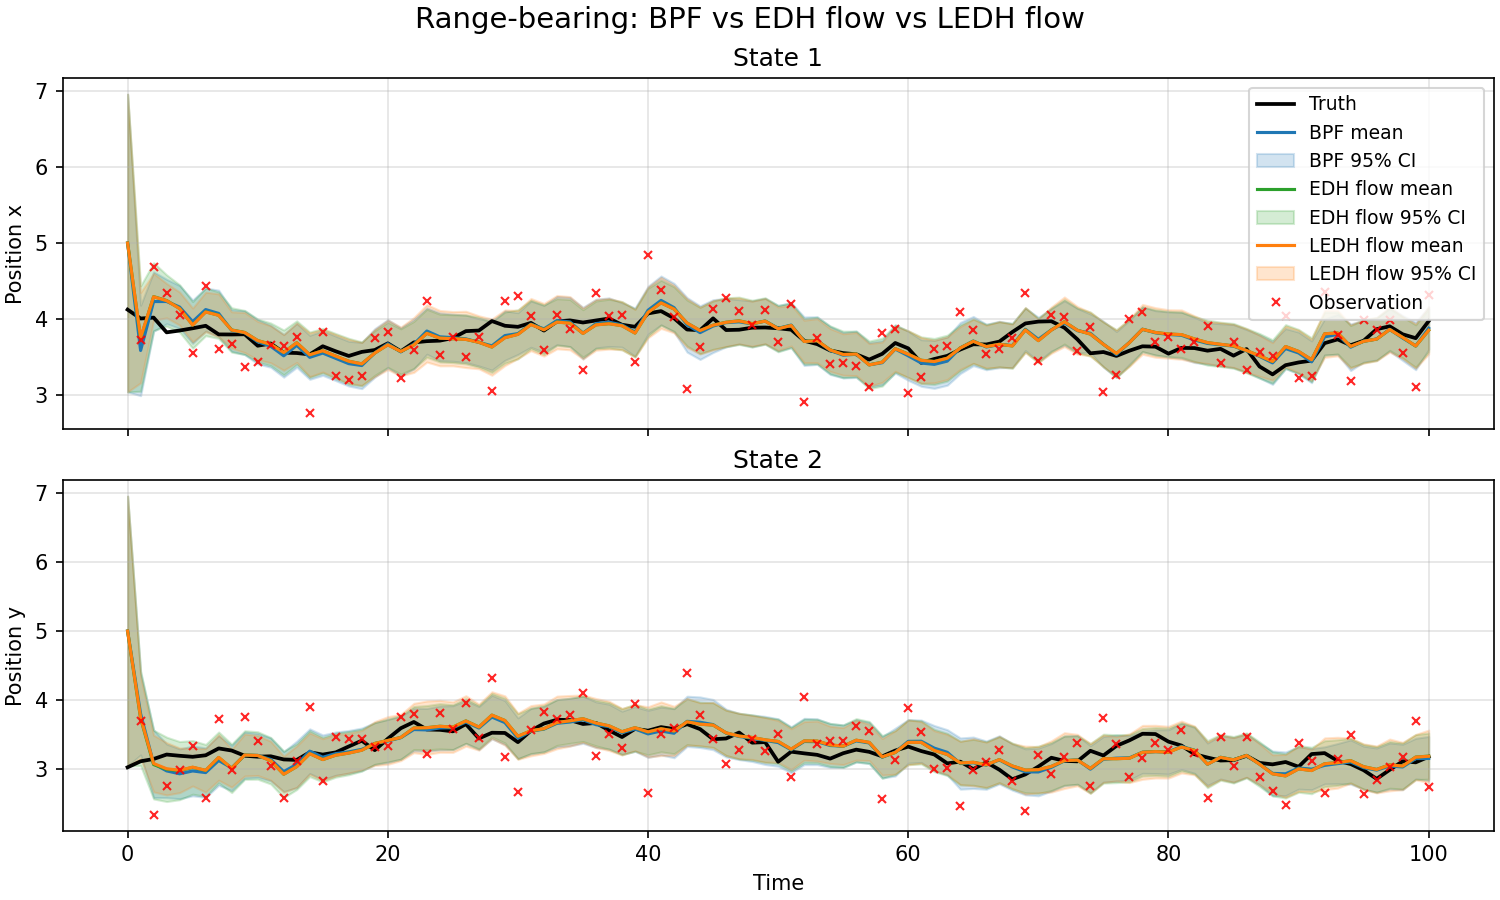
\includegraphics[width=0.9\linewidth]{pf_edh_ledh_rb.png}
    \caption{Range-bearing: bootstrap PF (blue), EDH flow (green), and LEDH flow (orange) overlaid on the true trajectory (black), with back-projected observations as red crosses. The three filters are visually indistinguishable on this well-conditioned model --- the per-model ranking in Table~\ref{tab:edh-rb} is driven primarily by wall-time; log-likelihood differs by a few nats but RMSE is tied to three decimal places.}
    \label{fig:pf_edh_ledh_rb}
\end{figure}

\begin{table}[H]
\centering
\footnotesize
\caption{Acoustic-tracking filter comparison ($T = 100$ except where noted). The high-dimensional state and weak observation geometry make this the hardest of the three headline models; none of the filters reach the same relative accuracy they do on range-bearing, and the ranking is driven as much by particle count and hyperparameter choice as by algorithm.}
\label{tab:edh-acoustic}
\begin{tabular}{lcccc}
\toprule
Filter & RMSE & Log-lik & Wall (s) & Notes \\
\midrule
EKF                          & $340.78$ & $-31166.52$ & $9.70$   & linearisation fails \\
UKF                          & $49.54$  & $-5421.08$  & $23.80$  &  \\
Bootstrap PF ($N=200$)       & $55.69$  & $+103.34$   & $8.15$   &  \\
Bootstrap PF ($N = 10^6, T=50$) & $22.13$ & $+610.82$  & $158.72$ & heavy particle compute \\
EDH flow                     & $297.46$ & $-24537.26$ & $36.25$  & diverges \\
EDH invertible               & $253.67$ & $-25126.02$ & $47.94$  & diverges \\
LEDH flow                    & $41.37$  & $-101415.40$& $48.59$  & best wall-time-to-RMSE \\
LEDH invertible              & $106.92$ & $-63810.64$ & $51.80$  &  \\
Stochastic EDH               & $45.11$  & $-65192.23$ & $24.79$  &  \\
\bottomrule
\end{tabular}
\end{table}

The acoustic result in Table~\ref{tab:edh-acoustic} is not the clean story I expected. LEDH-flow, not LEDH-invertible, is the best deterministic-flow variant on this model: $41.4$ RMSE against $106.9$ for the invertible sibling and ${\sim}255$--$297$ for the globally-linearised EDH variants. Stochastic EDH at $45.1$ is effectively tied with LEDH-flow. Bootstrap PF at a manageable $N = 200$ is cheaper but less accurate ($55.7$ RMSE in $8.15$ s); pushing to $N = 10^6$ (and shortening the trajectory to $T=50$) reaches $22.1$, which I treat as a brute-force reference rather than an operational point. The flow filters do not win wall-time here. They win RMSE at moderate compute.

\begin{table}[H]
\centering
\footnotesize
\caption{Stochastic volatility, \emph{raw} model ($h(x)=\beta e^{x/2}v$, multiplicative noise; $T=100$, $N=200$). Every linearisation-based method fails at ${\sim}2.0$ RMSE; only the bootstrap PF handles the raw multiplicative likelihood.}
\label{tab:edh-sv-raw}
\begin{tabular}{lccc}
\toprule
Filter & RMSE & Log-lik & Wall (s) \\
\midrule
Bootstrap PF            & $1.117$ & $\phantom{+}-68.12$  & $3.41$ \\
EDH flow                & $2.059$ & $-156.81$ & $13.17$ \\
Kernel (matrix)         & $2.091$ & --- & $101.02$ \\
\textit{Reference: EKF} & $2.039$ & $-151.20$ & $1.71$ \\
\textit{Reference: UKF} & $2.039$ & $-151.20$ & $1.90$ \\
\bottomrule
\end{tabular}
\end{table}

\begin{table}[H]
\centering
\footnotesize
\caption{Stochastic volatility, \emph{log-squared-transformed} model ($z = \log y^2$; $T=100$, $N=200$). The linear transform restores competitiveness to EKF/UKF and the flow family; kernel is slower but still tracks. LEDH-invertible is in the same narrow RMSE band as bootstrap PF, but does not beat it.}
\label{tab:edh-sv-log}
\begin{tabular}{lccc}
\toprule
Filter & RMSE & Log-lik & Wall (s) \\
\midrule
Bootstrap PF        & $1.153$ & $-235.63$ & $3.75$ \\
EDH flow            & $1.147$ & $-235.47$ & $14.38$ \\
LEDH invertible     & $1.162$ & $-236.25$ & $23.72$ \\
Kernel (matrix, $T=500$) & $1.372$ & --- & $287.39$ \\
\textit{Reference: EKF} & $1.144$ & $-235.27$ & $1.73$ \\
\textit{Reference: UKF} & $1.144$ & $-235.27$ & $1.95$ \\
\bottomrule
\end{tabular}
\end{table}

The SV takeaway: on the raw model, every filter that relies on a local linearisation of $h$ (EKF, UKF, EDH, LEDH, kernel) fails at the same ${\sim}2.0$ RMSE, and only the bootstrap PF --- which evaluates the likelihood directly without touching $h$'s Jacobian --- tracks the latent volatility. The log-squared transform flattens the ranking: RMSE compresses into a ${\sim}1.14$--$1.16$ band and the wall-time differences become the discriminator. EKF and UKF are again the cheap-and-good option; the flow filters are not wrong on this model, just unnecessary. Figure~\ref{fig:pf_edh_ledh_sv_log} shows the three-way comparison, and Figure~\ref{fig:edh_vs_ledh_flow_sv_log} isolates the EDH-vs-LEDH difference.

\begin{figure}[H]
    \centering
    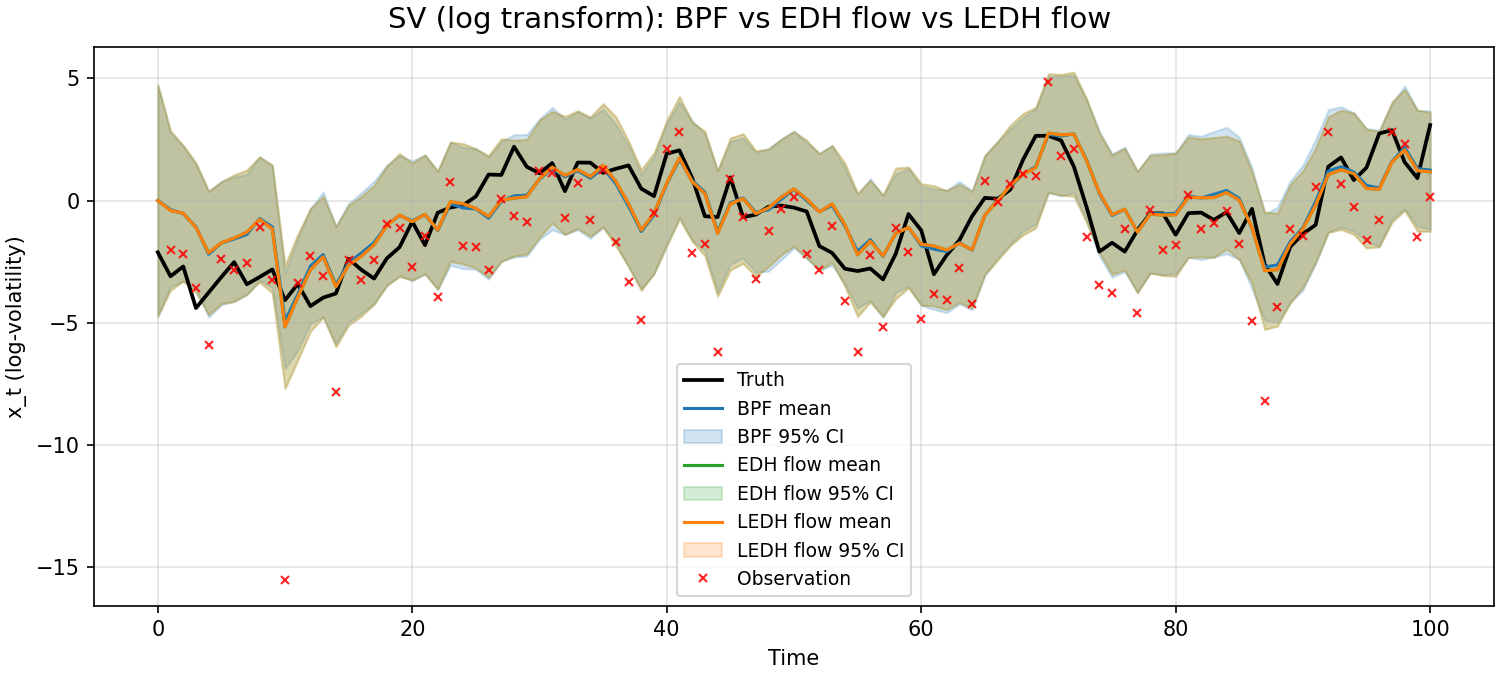
\includegraphics[width=0.85\linewidth]{pf_edh_ledh_sv_log.png}
    \caption{Log-squared stochastic volatility: bootstrap PF (blue), EDH flow (green), and LEDH flow (orange) compared against the true log-volatility (black) with back-projected observations as red crosses. After the log-squared transform, the three filters compress into a narrow band and the differences between them become invisible at this scale; the three filters all land in the same narrow RMSE band as the LEDH-invertible entry in Table~\ref{tab:edh-sv-log}.}
    \label{fig:pf_edh_ledh_sv_log}
\end{figure}

\begin{figure}[H]
    \centering
    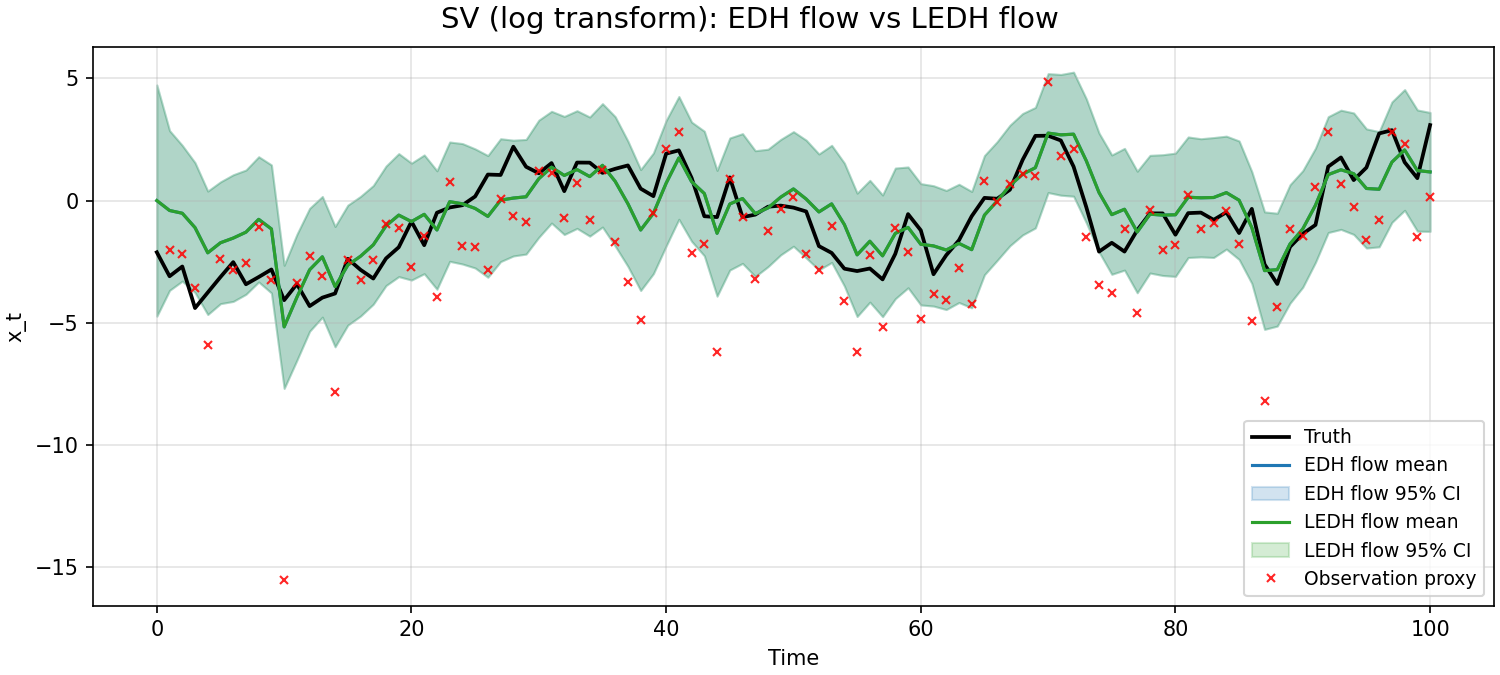
\includegraphics[width=0.85\linewidth]{edh_vs_ledh_flow_sv_log.png}
    \caption{Log-squared stochastic volatility, EDH flow (blue) vs.\ LEDH flow (green). The pairwise comparison isolates the effect of per-particle re-linearisation (LEDH) against a single global linearisation per time step (EDH) on the transformed model. Per-particle re-linearisation buys essentially nothing here: the two trajectories overlap within plot precision.}
    \label{fig:edh_vs_ledh_flow_sv_log}
\end{figure}

\paragraph{Stochastic volatility 2D (filter accuracy).}
SV2D reappears later as an HMC gradient-failure case (the chain has step-level gradient spikes and the multi-chain attempt crashed in the OT backward pass; see the Limitations summary). Before that, I record the filter-level result first. Figures~\ref{fig:pf_edh_ledh_sv2d}, \ref{fig:edh_flow_vs_invertible_sv2d}, and~\ref{fig:edh_vs_ledh_invertible_sv2d} compare bootstrap PF, EDH flow, LEDH flow, and the invertible counterparts of the flow variants on an SV2D trajectory with $N = 200$ particles and $T = 100$ time steps. A clean filter result on this model does not imply HMC will succeed on it, but a broken filter result would imply HMC cannot possibly succeed.

\begin{figure}[H]
    \centering
    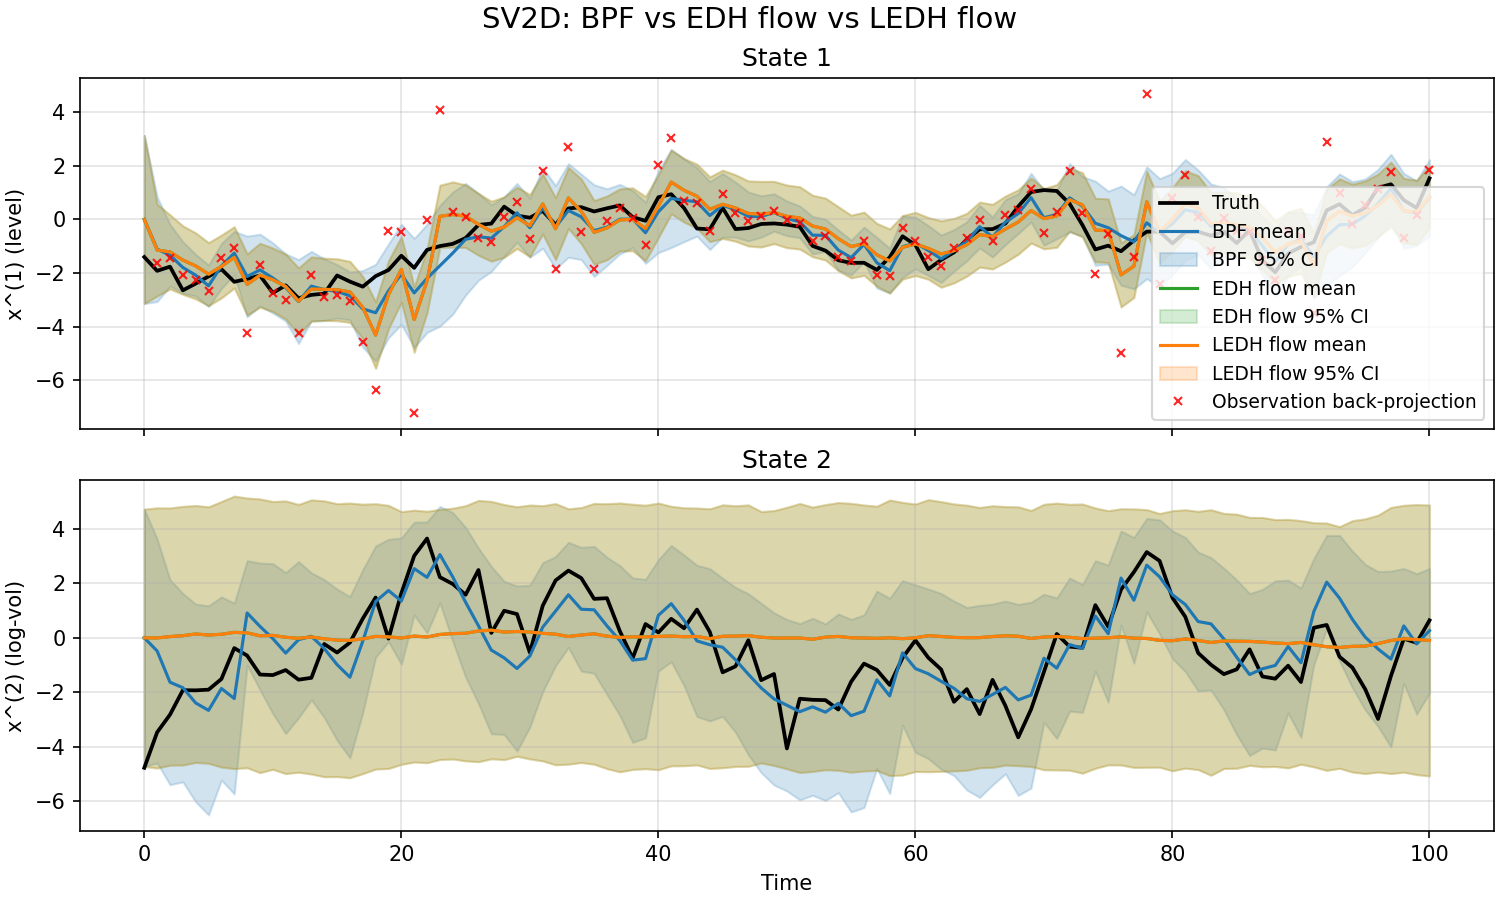
\includegraphics[width=0.9\linewidth]{pf_edh_ledh_sv2d.png}
    \caption{Stochastic volatility 2D: bootstrap PF (blue), EDH flow (green), LEDH flow (orange), overlaid on the true state (black). The first state component $x^{(1)}$ is the linear drift driver; the second $x^{(2)}$ is the log-volatility scale. Back-projected observations (red crosses) are shown only on the first panel because the SV2D observation model has a scalar output $y_t = b\,x_t^{(1)} + \exp(x_t^{(2)}/2)\,v_t$ with no per-dimension back-projection of $x^{(2)}$.}
    \label{fig:pf_edh_ledh_sv2d}
\end{figure}

\begin{figure}[H]
    \centering
    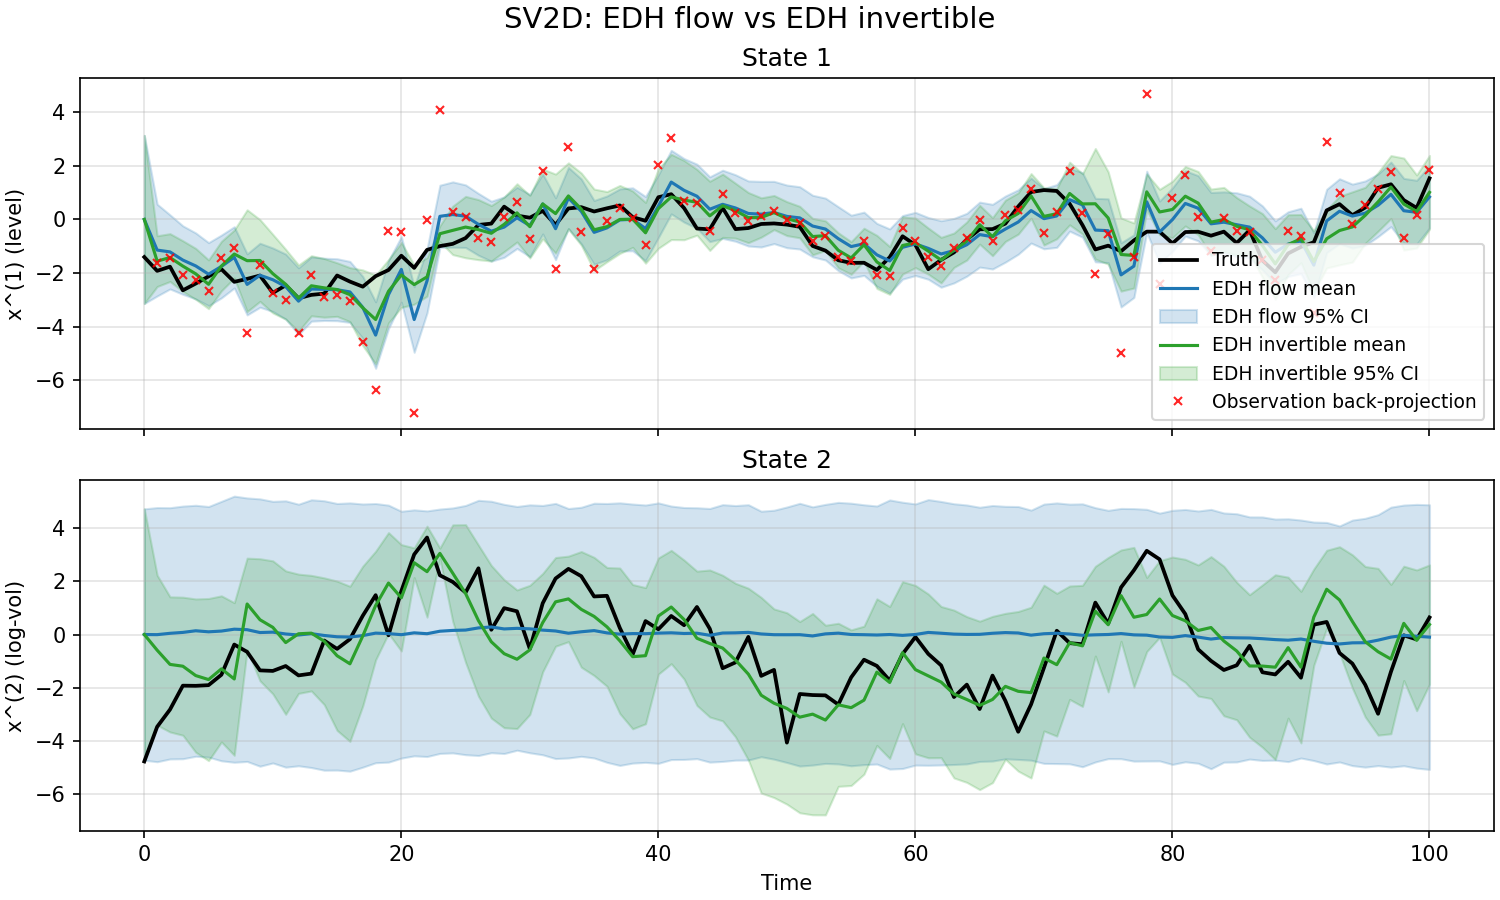
\includegraphics[width=0.9\linewidth]{edh_flow_vs_invertible_sv2d.png}
    \caption{Stochastic volatility 2D, EDH flow (blue) vs.\ EDH invertible (green). Both share the same global linearisation per time step; only the Jacobian correction differs. On this high-dimensional nonlinear target the two variants diverge visibly in places (max mean difference ${\approx}3.2$ in the log-volatility component), more than on range-bearing where the correction is essentially free.}
    \label{fig:edh_flow_vs_invertible_sv2d}
\end{figure}

\begin{figure}[H]
    \centering
    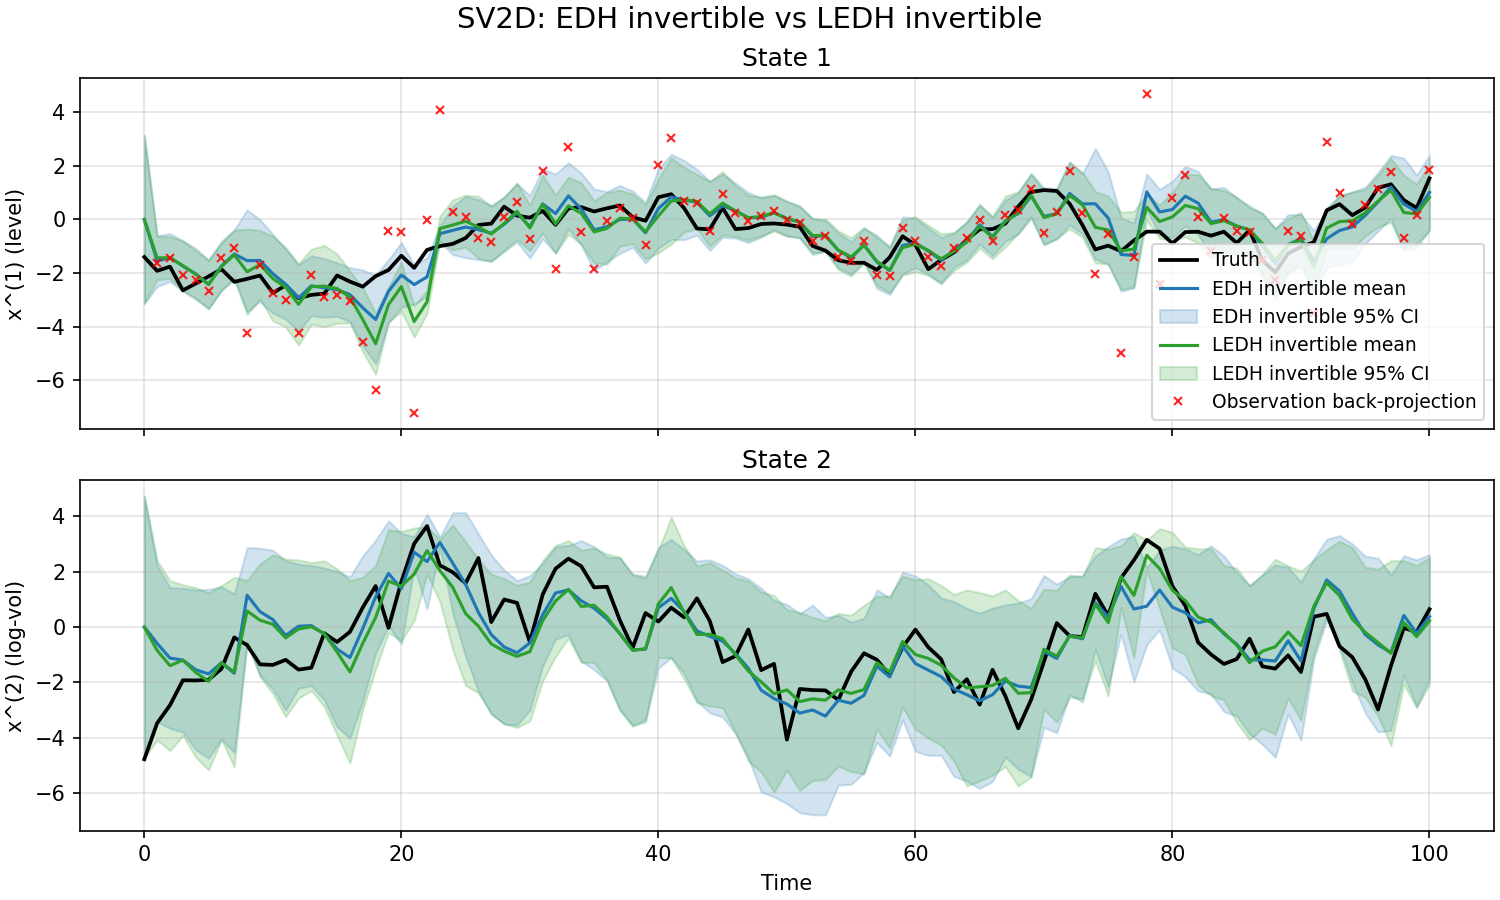
\includegraphics[width=0.9\linewidth]{edh_vs_ledh_invertible_sv2d.png}
    \caption{Stochastic volatility 2D, EDH invertible (blue) vs.\ LEDH invertible (green). Both carry the Jacobian correction; only the linearisation scheme differs (global vs.\ per-particle). On SV2D the per-particle LEDH variant is \emph{not} consistently better than global-EDH; the two filters cross each other in places and the ranking is not decisive.}
    \label{fig:edh_vs_ledh_invertible_sv2d}
\end{figure}

\subsection{Invertible Flow Filter}

\subsubsection{Why the Jacobian correction is needed}
The invertible flow filter \cite{Li-Particle-Filtering-2017} corrects for the volume distortion introduced by discretization. The continuous flow $d\v{x}/d\lambda = f(\v{x},\lambda)$ is exact by construction: the Fokker-Planck equation guarantees that following the flow moves probability mass correctly from $g(x)$ to $g(x)h(x)$. In practice I integrate with finite steps $\varepsilon_j$, so each $\lambda$ step applies the discrete affine map
\begin{equation}
    \boldsymbol{\eta}^{(i)} \;\leftarrow\; (I + \varepsilon_j A^{(i)}_j)\,\boldsymbol{\eta}^{(i)} + \varepsilon_j \mathbf{b}^{(i)}_j.
\end{equation}
This is an invertible linear map with Jacobian $\det(I + \varepsilon_j A^{(i)}_j)$. Unless $\det(I + \varepsilon_j A) = 1$ for every step (i.e., the map is volume-preserving), the discrete flow changes the volume element and therefore distorts the density. The continuous flow does not have this problem—the exact Fokker-Planck solution implicitly accounts for volume changes—but any finite discretization introduces this error. To correct for it, I re-introduce importance weights. The weight accumulated over all $n_\lambda$ steps of the flow at time $k$ is
\begin{equation}
    \log w_k^{(i)} = \log w_{k-1}^{(i)} + \sum_{j=1}^{n_\lambda} \log \bigl|\det\bigl(I + \varepsilon_j A^{(i)}_j\bigr)\bigr|,
    \label{eq:invertible_weight}
\end{equation}
which is then normalized across particles. A positive log-Jacobian means the map expanded the local volume (particles spread out), contributing upward weight; a negative one means compression, contributing downward weight. After the full flow the particle set $\{\boldsymbol{\eta}^{(i)}, w^{(i)}\}$ is a weighted approximation to the posterior, and the usual ESS-triggered resampling is applied.

For the EDH variants (both fixed and intermediate re-linearization), $A_j$ is a global matrix—the same for every particle at step $j$. The Jacobian factor $\det(I + \varepsilon_j A_j)$ is therefore identical for all particles. Under weight normalization, a common multiplicative factor in all $w^{(i)}$ cancels exactly. The relative weights remain uniform, and no correction is needed—the EDH flow filter without weights is already self-consistent. This is why the unweighted EDH flow (Algorithm~\ref{alg:edh_fixed} and~\ref{alg:edh_relinear}) is not simply an approximation that ignores the Jacobian; the Jacobian genuinely does not affect the normalized weights.

For LEDH, $A^{(i)}_j$ is particle-specific: different particles are linearized at different positions, so they are stretched or compressed by different amounts at each step. The Jacobian $\det(I + \varepsilon_j A^{(i)}_j)$ now varies across particles and does not cancel under normalization. Ignoring it would let the flow silently distort the distribution in a particle-dependent way. The invertible correction in~\eqref{eq:invertible_weight} accounts for exactly this: it reweights each particle by how much the flow expanded or contracted the space around it, restoring consistency between the transported point cloud and the target density.


At each $\lambda$ step, $A^{(i)} = -\tfrac{1}{2}\mathbf{P}\mathbf{H}^{(i)\top}(\lambda\mathbf{H}^{(i)}\mathbf{P}\mathbf{H}^{(i)\top}+\mathbf{R})^{-1}\mathbf{H}^{(i)}$ has rank at most $d_z$ (the observation dimension), because it is a product $UW V^\top$ where $U = \mathbf{P}\mathbf{H}^{(i)\top}$ is $d_x \times d_z$. A naive determinant over $d_x \times d_x$ matrices would be expensive. Instead, apply Sylvester's determinant theorem $\det(I_{d_x} + UV^\top) = \det(I_{d_z} + V^\top U)$ to reduce the computation to a $d_z \times d_z$ determinant:
\begin{equation}
    \log\bigl|\det(I_{d_x} + \varepsilon_j A^{(i)})\bigr|
    = \log\bigl|\det\!\bigl(I_{d_z} - \tfrac{\varepsilon_j}{2}\,\mathbf{H}^{(i)}\mathbf{P}\mathbf{H}^{(i)\top}(\lambda\mathbf{H}^{(i)}\mathbf{P}\mathbf{H}^{(i)\top}+\mathbf{R})^{-1}\bigr)\bigr|.
\end{equation}
When $d_z \ll d_x$ this is a substantial saving. In the common case $d_z = d_x = 1$ it reduces to a scalar logarithm. The accumulated log-weight over all $n_\lambda$ steps is computed by summing this scalar (or small-matrix determinant) at each step, adding negligible overhead compared to the flow integration itself.

\begin{algorithm}[H]
\caption{EDH Invertible Particle Flow Filter (Intermediate Re-linearization)}
\begin{algorithmic}[1]
\REQUIRE Particles $\{\boldsymbol{\eta}^{(i)}, w^{(i)}\}_{i=1}^N$, parallel EKF/UKF, ESS threshold
\FOR{$k = 1, 2, \ldots, T$}
  \STATE \textbf{Predict (EKF/UKF):} $(\bar{\boldsymbol{\eta}}_0, \mathbf{P}) \leftarrow \text{EKF/UKF predict}$
  \STATE \textbf{Predict (particles):} $\boldsymbol{\eta}_0^{(i)} \sim p(\mathbf{x}_k \mid \boldsymbol{\eta}^{(i)})$, store pre-flow particles
  \STATE Precompute $\mathbf{R}^{-1}$
  \STATE Initialize $\lambda \leftarrow 0$, $\boldsymbol{\eta}_1^{(i)} \leftarrow \boldsymbol{\eta}_0^{(i)}$, $\bar{\boldsymbol{\eta}}^{(\lambda)} \leftarrow \bar{\boldsymbol{\eta}}_0$
  \FOR{$j = 1, 2, \ldots, n_\lambda$}
    \STATE $\lambda \leftarrow \lambda + \varepsilon_j$
    \STATE $\mathbf{H} \leftarrow \frac{\partial \mathbf{h}}{\partial \mathbf{x}}\Big|_{\bar{\boldsymbol{\eta}}^{(\lambda)}}$ \hfill (re-linearize at current global mean)
    \STATE $\mathbf{e} \leftarrow \mathbf{h}(\bar{\boldsymbol{\eta}}^{(\lambda)}) - \mathbf{H}\bar{\boldsymbol{\eta}}^{(\lambda)}$ \hfill (nonlinear correction)
    \STATE $\mathbf{A} \leftarrow -\tfrac{1}{2}\mathbf{P}\mathbf{H}^\top(\lambda\mathbf{H}\mathbf{P}\mathbf{H}^\top + \mathbf{R})^{-1}\mathbf{H}$
    \STATE $\mathbf{b} \leftarrow (\mathbf{I}+2\lambda\mathbf{A})[(\mathbf{I}+\lambda\mathbf{A})\mathbf{P}\mathbf{H}^\top\mathbf{R}^{-1}(\mathbf{z}_k - \mathbf{e}) + \mathbf{A}\bar{\boldsymbol{\eta}}_0]$
    \STATE $\bar{\boldsymbol{\eta}}^{(\lambda)} \leftarrow \bar{\boldsymbol{\eta}}^{(\lambda)} + \varepsilon_j(\mathbf{A}\bar{\boldsymbol{\eta}}^{(\lambda)} + \mathbf{b})$ \hfill (advance mean for next step)
    \STATE $\boldsymbol{\eta}_1^{(i)} \leftarrow \boldsymbol{\eta}_1^{(i)} + \varepsilon_j(\mathbf{A}\boldsymbol{\eta}_1^{(i)} + \mathbf{b})$ for all $i$
  \ENDFOR
  \STATE \textbf{Weight update:}
  \STATE $\tilde{w}^{(i)} \leftarrow w^{(i)} \cdot \frac{p(\mathbf{z}_k \mid \boldsymbol{\eta}_1^{(i)})}{p(\mathbf{z}_k \mid \boldsymbol{\eta}_0^{(i)})}$ \hfill (importance weight correction)
  \STATE $w^{(i)} \leftarrow \tilde{w}^{(i)} / \sum_j \tilde{w}^{(j)}$ \hfill (normalize)
  \STATE $\boldsymbol{\eta}^{(i)} \leftarrow \boldsymbol{\eta}_1^{(i)}$
  \IF{$N_{\text{eff}} = 1/\sum_i (w^{(i)})^2 < \text{threshold}$}
    \STATE Resample $\{\boldsymbol{\eta}^{(i)}, w^{(i)}\}$ \hfill (systematic resampling)
  \ENDIF
  \STATE \textbf{Update (EKF/UKF):} $(\bar{\boldsymbol{\eta}}, \mathbf{P}) \leftarrow \text{EKF/UKF update}(\bar{\boldsymbol{\eta}}_0, \mathbf{P}, \mathbf{z}_k)$
\ENDFOR
\end{algorithmic}
\end{algorithm}

\begin{algorithm}[H]
\caption{LEDH Invertible Particle Flow Filter (Local Linearization + Jacobian Tracking)}
\begin{algorithmic}[1]
\REQUIRE Particles $\{\boldsymbol{\eta}^{(i)}, w^{(i)}\}_{i=1}^N$, per-particle batched EKF/UKF, ESS threshold
\REQUIRE Weight clip range $C$ (optional, e.g.\ $C=50$)
\FOR{$k = 1, 2, \ldots, T$}
  \STATE \textbf{Predict (batched EKF/UKF):}
  \STATE $(\bar{\boldsymbol{\eta}}_0^{(i)}, \mathbf{P}^{(i)}) \leftarrow \text{batched EKF/UKF predict}(\boldsymbol{\eta}^{(i)}, \mathbf{P}^{(i)})$ for all $i$
  \STATE \textbf{Predict (particles):} $\boldsymbol{\eta}_0^{(i)} \sim p(\mathbf{x}_k \mid \boldsymbol{\eta}^{(i)})$
  \STATE Precompute $\mathbf{R}^{-1}$
  \STATE Initialize $\lambda \leftarrow 0$, $\boldsymbol{\eta}_1^{(i)} \leftarrow \boldsymbol{\eta}_0^{(i)}$, $\log\theta^{(i)} \leftarrow 0$
  \FOR{$j = 1, 2, \ldots, n_\lambda$}
    \STATE $\lambda \leftarrow \lambda + \varepsilon_j$
    \FOR{each particle $i$ (batched)}
      \STATE $\mathbf{H}^{(i)} \leftarrow \frac{\partial \mathbf{h}}{\partial \mathbf{x}}\Big|_{\boldsymbol{\eta}_1^{(i)}}$ \hfill (re-linearize at current position)
      \STATE $\mathbf{e}^{(i)} \leftarrow \mathbf{h}(\boldsymbol{\eta}_1^{(i)}) - \mathbf{H}^{(i)}\boldsymbol{\eta}_1^{(i)}$
      \STATE Compute $\mathbf{A}^{(i)}(\lambda), \mathbf{b}^{(i)}(\lambda)$ using $\mathbf{H}^{(i)}, \mathbf{P}^{(i)}, \bar{\boldsymbol{\eta}}_0^{(i)}$
    \ENDFOR
    \STATE $\boldsymbol{\eta}_1^{(i)} \leftarrow \boldsymbol{\eta}_1^{(i)} + \varepsilon_j(\mathbf{A}^{(i)}\boldsymbol{\eta}_1^{(i)} + \mathbf{b}^{(i)})$ for all $i$
    \STATE $\mathbf{M}^{(i)} \leftarrow \mathbf{I} + \varepsilon_j \mathbf{A}^{(i)}$ \hfill (local Jacobian of flow map)
    \STATE $\log\theta^{(i)} \leftarrow \log\theta^{(i)} + \log|\det(\mathbf{M}^{(i)})|$ \hfill (accumulate log-det)
  \ENDFOR
  \STATE \textbf{Weight update with Jacobian correction:}
  \STATE $\log\theta^{(i)} \leftarrow \log\theta^{(i)} - \max_j \log\theta^{(j)}$ \hfill (stabilize before exp)
  \STATE $\theta^{(i)} \leftarrow \exp(\log\theta^{(i)})$
  \STATE $\tilde{w}^{(i)} \leftarrow w^{(i)} \cdot \frac{p(\mathbf{z}_k \mid \boldsymbol{\eta}_1^{(i)})}{p(\mathbf{z}_k \mid \boldsymbol{\eta}_0^{(i)})} \cdot \theta^{(i)}$
  \IF{clip range $C$ specified}
    \STATE $\log \tilde{w}^{(i)} \leftarrow \text{clip}(\log \tilde{w}^{(i)},\; -C,\; +C)$ \hfill (prevent overflow)
  \ENDIF
  \STATE $w^{(i)} \leftarrow \tilde{w}^{(i)} / \sum_j \tilde{w}^{(j)}$
  \STATE $\boldsymbol{\eta}^{(i)} \leftarrow \boldsymbol{\eta}_1^{(i)}$
  \STATE \textbf{Update (batched EKF/UKF):} update per-particle covariances
  \IF{$N_{\text{eff}} < \text{threshold}$}
    \STATE Resample $\{\boldsymbol{\eta}^{(i)}, w^{(i)}\}$
  \ENDIF
\ENDFOR
\end{algorithmic}
\end{algorithm}

\paragraph{When does the Jacobian correction help?} 

The Jacobian correction is harmless on range-bearing and should help on high-dimensional targets, but on acoustic tracking it is strictly worse than uncorrected LEDH in my runs. Figures~\ref{fig:edh_flow_vs_invertible_rb} and~\ref{fig:ledh_flow_vs_invertible_rb} show the range-bearing control case. I defer the root-cause investigation to future work --- the most likely culprits are float32 precision on the per-particle Cholesky and the log-determinant clipping I use for stability.

\begin{figure}[H]
    \centering
    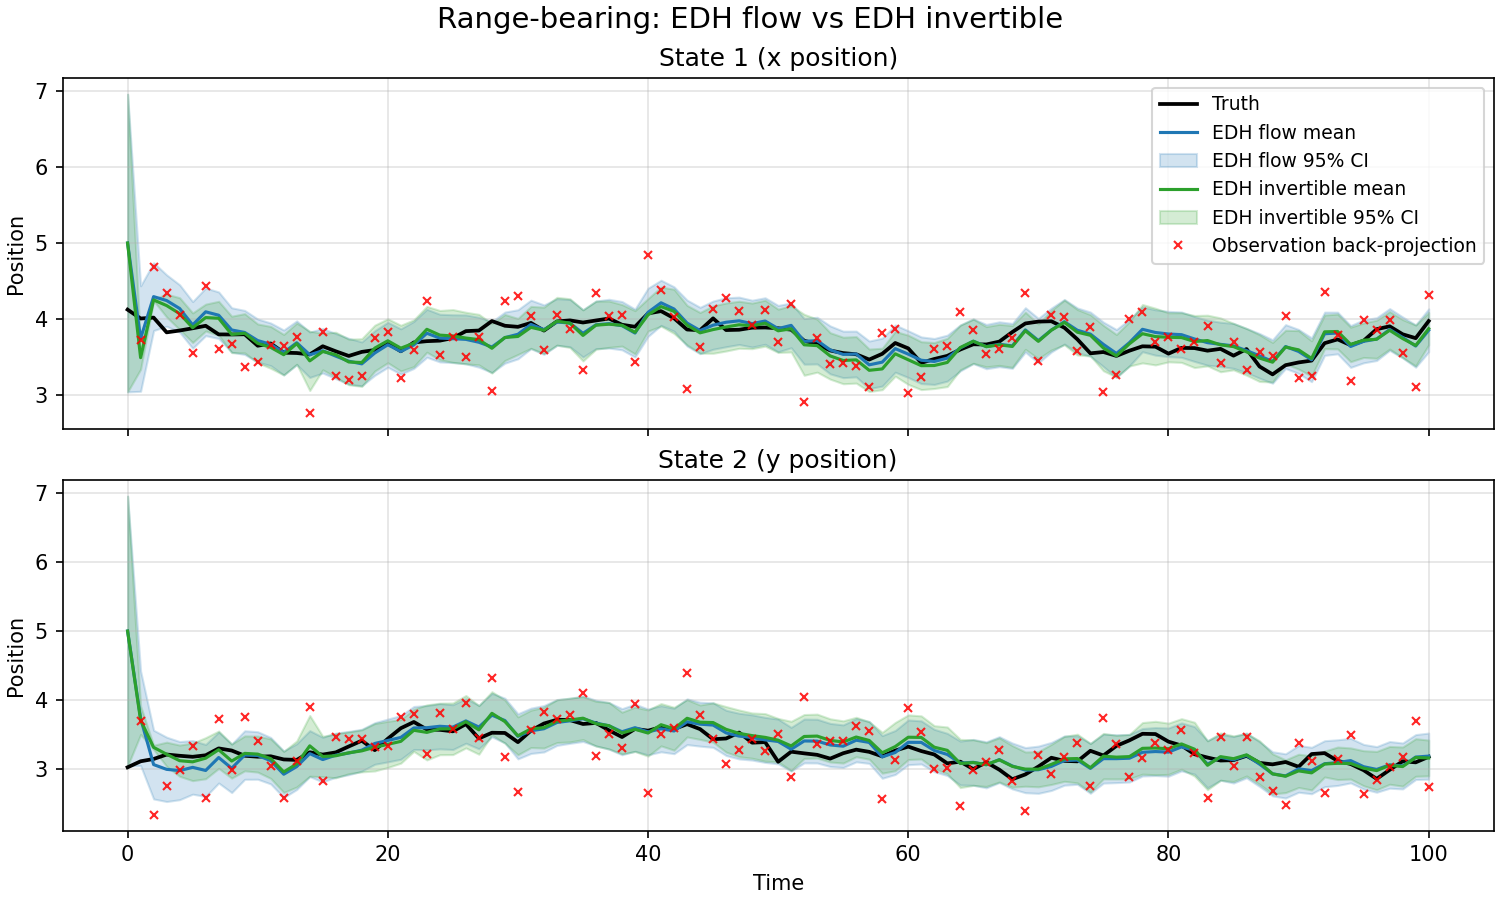
\includegraphics[width=0.9\linewidth]{edh_flow_vs_invertible_rb.png}
    \caption{Range-bearing, EDH flow (blue) vs.\ EDH invertible (green). The two variants are visually indistinguishable: on this well-conditioned 2D model the per-particle log-determinants are close to unity at every flow step, so the Jacobian correction adds negligible information and adds negligible error. This is the control that says the correction is numerically harmless in the easy regime.}
    \label{fig:edh_flow_vs_invertible_rb}
\end{figure}

\begin{figure}[H]
    \centering
    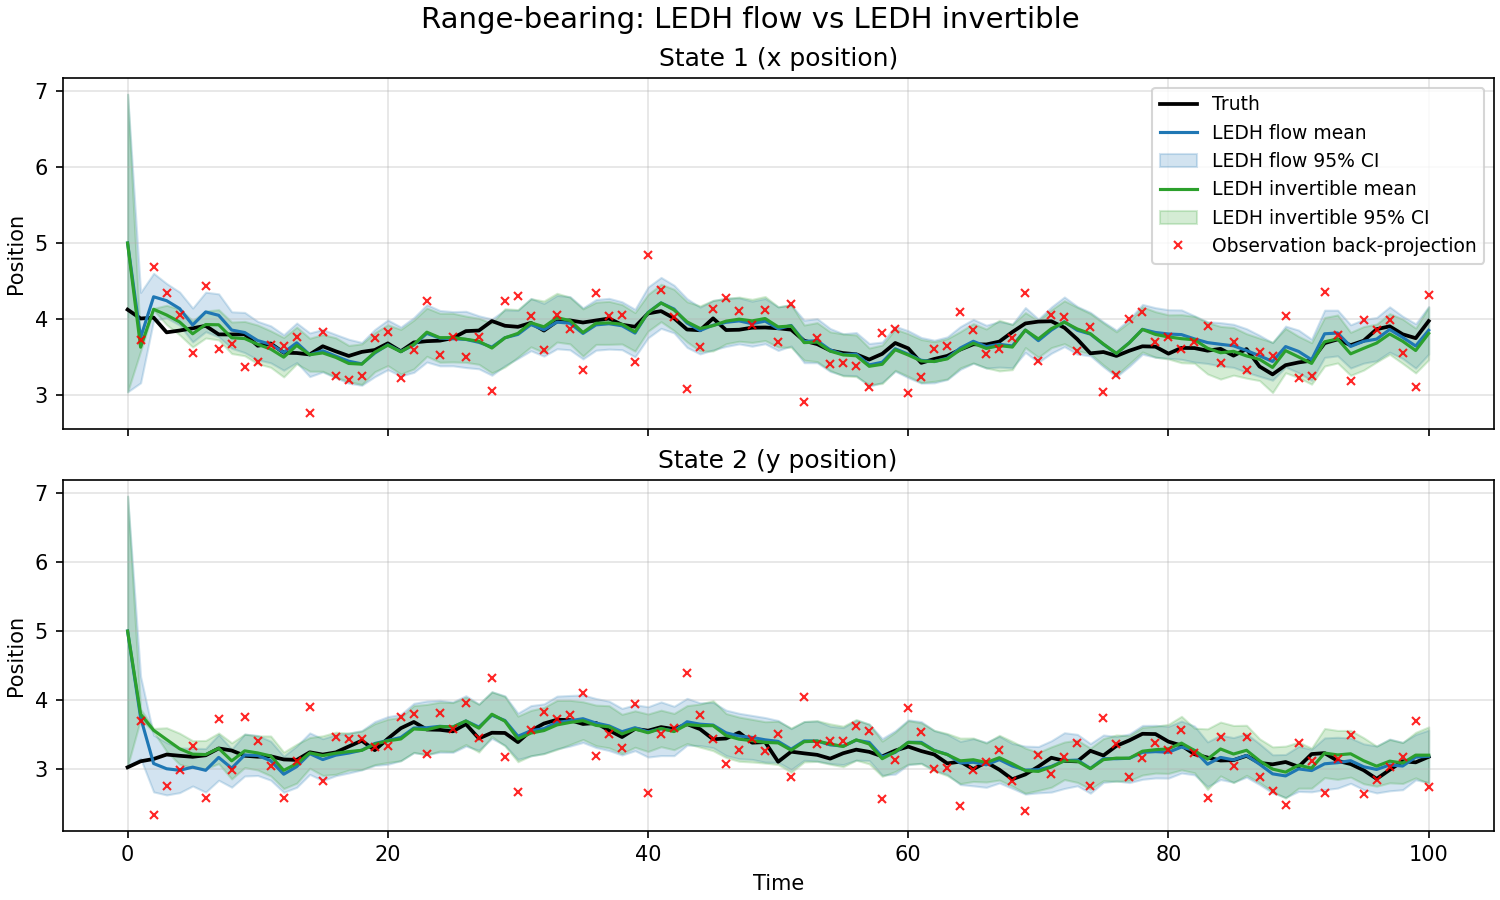
\includegraphics[width=0.9\linewidth]{ledh_flow_vs_invertible_rb.png}
    \caption{Range-bearing, LEDH flow (blue) vs.\ LEDH invertible (green). The per-particle-linearisation version of the same comparison. Conclusion is identical: on a well-conditioned low-dimensional model the invertible correction neither helps nor hurts, and the empirical tie holds whether the underlying linearisation is global or local.}
    \label{fig:ledh_flow_vs_invertible_rb}
\end{figure}


%Two observations from the experiments in \S\ref{sec:edh-experiments}. First, on the range-bearing model the invertible and uncorrected LEDH variants are essentially tied on RMSE (both ${\approx}0.13$); accumulating $n_\lambda$ log-determinants across many $\lambda$ steps on a well-conditioned 2D problem does not hurt, but it does not buy useful headroom either --- the per-particle Jacobians are already close to unity. Second, on the high-dimensional acoustic-tracking model the correction is \emph{not} a clean win: LEDH-flow reaches RMSE ${\approx}41$ while LEDH-invertible sits at ${\approx}107$. One interpretation is that the Jacobian accumulation injects variance that swamps the theoretical benefit on long trajectories in high dimension; another is that the log-determinant clipping we use for numerical stability silently discards the very gradient information the correction is supposed to provide. This is an open question --- the invertible correction is the right thing theoretically, but on acoustic tracking it does not yet deliver in our implementation.

\subsection{Stochastic Flow Filter}

I used the stochastic particle flow filter of \cite{dai-new-2021} as the SDE analogue of deterministic EDH:
\[
  d\v{x} = \bigl[A(\lambda)\v{x} + b(\lambda)\bigr]\,d\lambda + \sqrt{Q}\,dW_\lambda,
\]
Here $Q = \operatorname{diag}(q_1,\ldots,q_d)$ is diagonal. The extra noise is not free. The drift needs the score correction from Corollary~2.1 of \cite{dai-new-2021}; otherwise the particles diffuse away from the homotopy density.

Deterministic EDH can re-linearise $H$ at each particle. That is the LEDH idea. Each particle follows its own ODE velocity field, so this is well-defined. The stochastic case is stricter. The drift contains a score term:
\[
  f_{\mathrm{stoch}}(\v{x},\lambda)
  = f_{\mathrm{det}}(\v{x},\lambda)
    + \tfrac{1}{2}\,Q\;\nabla_{\v{x}} \log p(\v{x},\lambda),
\]
where $p(\v{x},\lambda) \propto g(\v{x})\,h(\v{x})^{\lambda}$. The point is not the formula itself. The point is that the score must come from one density shared by all particles. The drift must satisfy
\[
  \frac{\partial p}{\partial\lambda}
  = -\nabla\!\cdot\!(f\,p) + \tfrac{1}{2}\nabla\!\cdot\!\bigl(QQ^\top \nabla p\bigr),
\]
a \emph{global} constraint. There must be one density $p(\v{x},\lambda)$ whose score drives every particle at the same pseudo-time.

With global linearisation, $H$ is fixed at $\bar\eta_0$. Then the homotopy density is Gaussian with precision $M(\lambda) = P_0^{-1} + \lambda\,H^\top R^{-1}H$, and the score
\[
  \nabla\log p(\v{x},\lambda) = -M(\lambda)\bigl(\v{x} - m(\lambda)\bigr)
\]
is one linear function of $\v{x}$. This is why the Fokker--Planck argument still goes through.

If I re-linearise at each particle $\v{x}_i$, particle~$i$ gets its own $H_i$, precision $M_i(\lambda)$, mean $m_i(\lambda)$, and score $-M_i(\v{x} - m_i)$. No single density has all of those scores. The particles stop representing one coherent density, so the stochastic-flow guarantee is gone. This is why the stochastic-flow literature uses global linearisation, and why LEDH-style local re-linearisation belongs to deterministic flows. In code, I kept the EDH structure and only changed the flow parameters. For nonlinear observations, I cannot keep updating $H$ during the stochastic flow. The workaround is a local correction term.

The drift formulas assume $h(\v{x}) = H\v{x}$. If the observation is actually linear, computing $H$ once at $\bar\eta_0$ is enough.

For nonlinear observations, the Taylor expansion at a point $\eta$ gives
\[
  h(\v{x}) \approx h(\eta) + H(\eta)(\v{x} - \eta) = H(\eta)\v{x} + \underbrace{\bigl[h(\eta) - H(\eta)\,\eta\bigr]}_{e},
\]
The residual $e$ is the nonlinear part that the global linear model misses. I borrow this from LEDH but do not re-linearise during the stochastic flow. I compute $e_0 = h(\bar\eta_0) - H\bar\eta_0$ once and replace $z$ by $z_{\mathrm{corr}} = z - e_0$ in both the deterministic drift and the score correction. For linear observations, $e_0 = 0$.

This correction is essential on nonlinear models. On range-bearing, uncorrected stochastic EDH diverges. The local correction makes the same filter work (Figure~\ref{fig:rb_sde_combined}). It costs one extra evaluation of $h(\bar\eta_0)$ per time step.
The flow is stiff near $\lambda = 0$. There, $M(\lambda) = P_0^{-1} + \lambda\,H^\top R^{-1} H$ is still dominated by the anisotropic prior. Near $\lambda = 1$, the measurement term regularises the precision and the stiffness weakens. A fine uniform grid keeps Euler--Maruyama stable, so the stiffness is not fatal if the step size is small enough.

I used a geometric schedule in practice: $\varepsilon_j = \varepsilon_1 q^{j-1}$ with $q = 1.2$. This puts small steps near $\lambda = 0$ and larger steps near $\lambda = 1$. It solved the practical stiffness issue without an optimisation problem. I spent time trying to reproduce the stiffness-mitigation result of \cite{ding2012implementation}, but I could not reproduce it. The filter worked. The proposed schedule did not give a useful gain in my runs; a fine uniform grid or the geometric heuristic was enough. I did not try changing the integration scheme. I also followed the pseudocode and evaluated the parameters after updating the step count. Since the first step is the stiffest one, this ordering may explain why I could not reproduce the paper.

\begin{figure}[H]
  \centering
  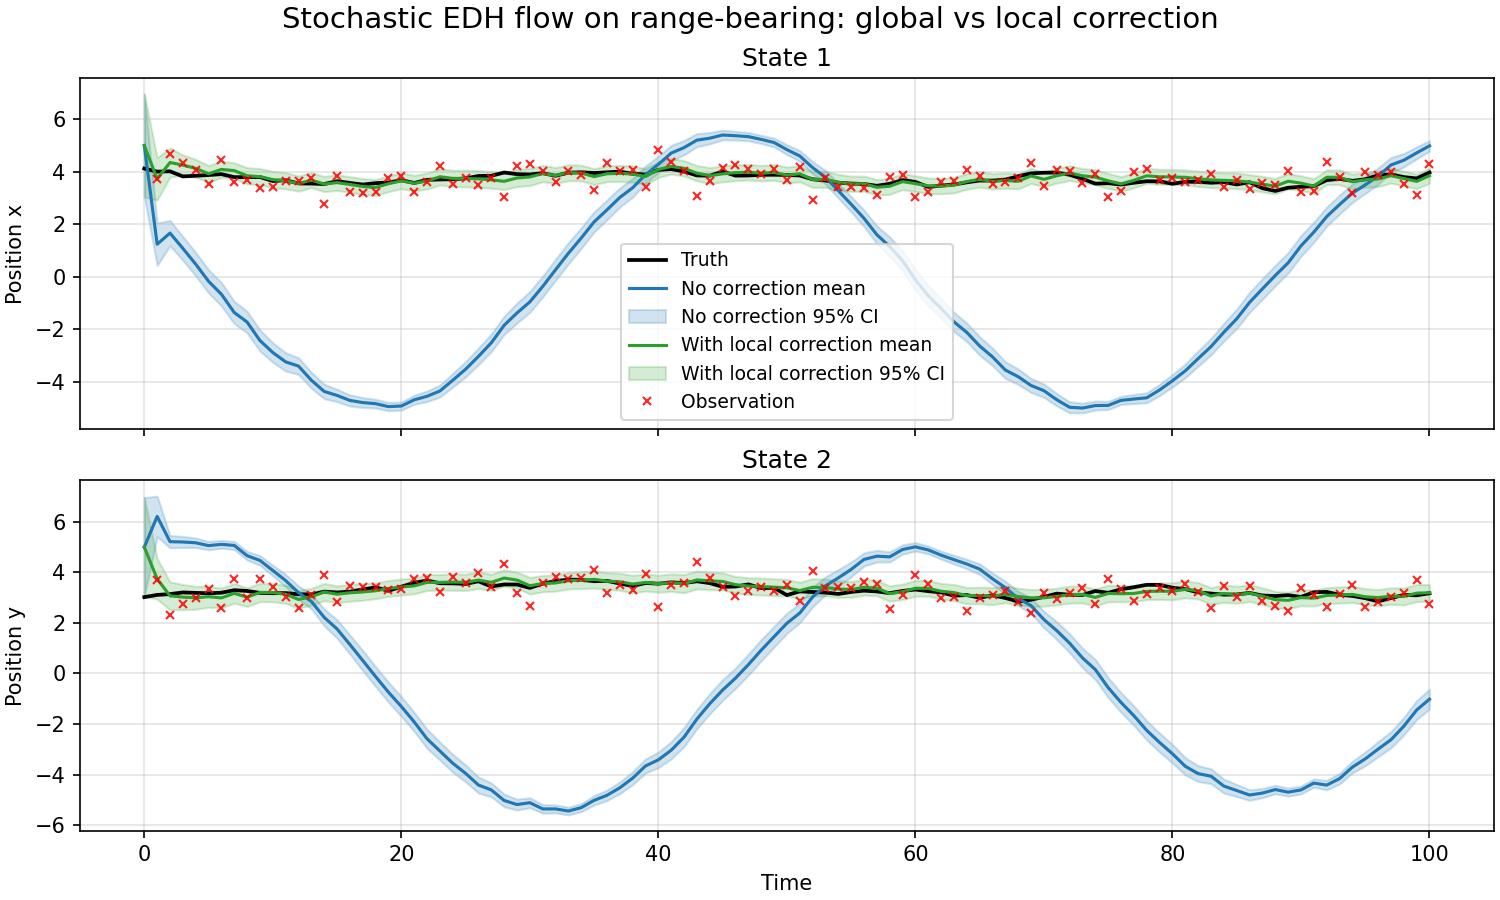
\includegraphics[width=0.9\textwidth]{stochastic_edh_rb_combined.png}
  \caption{Stochastic EDH flow on the range-bearing model: no correction (blue, RMSE $\approx 5.28$) versus with local correction $e_0 = h(\bar{\boldsymbol{\eta}}_0) - \mathbf{H}\bar{\boldsymbol{\eta}}_0$ (green, RMSE $\approx 0.13$). True trajectory in black; observations as red crosses back-projected to position coordinates. The uncorrected run diverges because the global linearisation is stale throughout the flow; adding the local correction makes the same drift equation track the truth within one position unit.}
  \label{fig:rb_sde_combined}
\end{figure}


\begin{table}[H]
\centering
\footnotesize
\caption{Stochastic EDH on the range-bearing model. `No correction' means $e_0 = 0$ and the drift is derived under pure global linearisation; `+ local correction' uses $e_0 = h(\bar\eta_0) - H\bar\eta_0$. `100 steps' forces a uniform $n_\lambda = 100$ grid; `optimal' uses the stiffness-mitigation schedule of \cite{ding2012implementation}.}
\label{tab:sde_flow}
\begin{tabular}{lccc}
\toprule
Variant & RMSE & Log-lik & Wall (s) \\
\midrule
No correction, default $n_\lambda$    & $5.276$ & $-17401.29$ & $129.17$ \\
No correction, $n_\lambda = 100$       & $1.307$ & $-23799.91$ & $104.78$ \\
No correction, optimal schedule         & $1.307$ & $-23780.79$ & $414.63$ \\
+ local correction, default $n_\lambda$ & $0.131$ & $+110.06$   & $128.74$ \\
+ local correction, $n_\lambda = 100$  & $0.252$ & $-146.90$   & $106.97$ \\
+ local correction, optimal schedule     & $0.131$ & $+110.10$   & $359.14$ \\
%\midrule
%\textit{Reference: Kalman filter}       & $5.276$ & --- & --- \\
%\textit{Reference: deterministic EDH flow} & $0.132$ & $+110.13$ & $130.41$ \\
\bottomrule
\end{tabular}
\end{table}

\paragraph{Empirical takeaway (§4.5).} Three facts from Table~\ref{tab:sde_flow}. (i)~Without the local correction $e_0$, stochastic flow on the range-bearing model is as bad as the Kalman filter on the same task --- the uncorrected drift diverges or tracks the prior mean, because the linearisation is stale throughout the flow. (ii)~With the local correction, the default stochastic EDH run works (RMSE $=0.131$), but it does \emph{not} beat the deterministic EDH/LEDH flows, which already reach comparable or better RMSE at a fraction of the compute. The $n_\lambda=100$ variant settles near $0.25$. (iii)~The `optimal' step-size schedule of \cite{ding2012implementation} did not help in my runs: I could not reproduce the stiffness-mitigation gain, and a fine uniform schedule plus the geometric-ratio heuristic was sufficient. 

\clearpage
\subsection{Kernel Flow Filter}

\subsubsection{Overview}
Kernel flow replaces the affine drift with an RKHS velocity field \cite{Pulido2019,HuVanLeeuwen2021}. Instead of moving particles along a fixed affine schedule, I move them in the direction that decreases the gap between the particle density and the target as quickly as possible.
Define the target posterior $\pi(x) := p(x_t | z_{1:t})$ and the intermediate density $q_\lambda(x)$ at pseudo-time $\lambda \in [0,1]$. The endpoints are $q_0 = p(x_t | z_{1:t-1})$ and $q_1 = \pi$.
\begin{equation}
\frac{dx_\lambda}{d\lambda} = v_\lambda(x_\lambda)
\end{equation}
Choose $v_\lambda$ to decrease the KL divergence as fast as possible:
\begin{equation}
D_{KL}(q_\lambda \| \pi) = \int q_\lambda(x) \log \frac{q_\lambda(x)}{\pi(x)} dx
\end{equation}
For the code, I needed a computable drift. The intuition is simple: move each point along the steepest descent direction for this density mismatch.

  



\subsubsection{Derivation}


%Our problem is the same as particle filter particle flow, move the particles to the desired location, without touching the weights, so that we get the target probability distribution $p(x_t | y_{1:t}) \propto p(y_t | x_t) p(x_t | y_{1:t-1})$. 

%\paragraph{Optimal Transport via Gradient Flow}

%Define target posterior $\pi(x) := p(x_t | y_{1:t})$ and intermediate density $q_\lambda(x)$ at pseudo-time $\lambda \in [0,1]$. With $q_0 = p(x_t | y_{1:t-1})$ (prior), $q_1 = \pi$ (posterior).
%\begin{equation}
%\frac{dx_\lambda}{d\lambda} = v_\lambda(x_\lambda)
%\%%end{equation}
%Choose velocity $v_\lambda$ to minimize KL divergence as fast as possible:
%\begin{equation}
%D_{KL}(q_\lambda \| \pi) = \int q_\lambda(x) \log \frac{q_\lambda(x)}{\pi(x)} dx
%\end{equation}
%we need to formulate the above equation into an optimization problem. But the intuition of this method is clear, you want to evolve the point along a "straight" direction to the desire point. 


\paragraph{Deriving Optimal Velocity via Kernel Restriction.}
Under velocity field $v$, the density evolves by the Liouville equation:
\begin{equation}
\frac{\partial q_\lambda}{\partial \lambda} = -\nabla_x \cdot (q_\lambda v)
\end{equation}

Differentiate $D_{KL}$ in pseudo-time:
\begin{align}
\frac{d}{d\lambda} D_{KL} &= \int \frac{\partial q_\lambda}{\partial \lambda} \left[\log q_\lambda(x) - \log \pi(x) + 1\right] dx \\
&= -\int \nabla_x \cdot (q_\lambda v) \left[\log q_\lambda(x) - \log \pi(x) + 1\right] dx
\end{align}

Using $\nabla_x q_\lambda = q_\lambda \nabla_x \log q_\lambda$ and integrating by parts:
\begin{equation}
\frac{d}{d\lambda} D_{KL} = -\int q_\lambda \left[\nabla_x \log \pi(x) \cdot v + \nabla_x \cdot v\right] dx 
\end{equation}

The derivative gives the vector field along the trajectory. To make it computable, I restrict $v$ to functions generated by a kernel $K(x,x')$. Any such function has the form:
\begin{equation}
v(x) = \int \alpha(x') K(x', x) dx'
\end{equation}
for some coefficient function $\alpha(x')$. I substitute this into the directional derivative.

\begin{align}
\frac{d}{d\lambda}D_{KL} &= -\int q_\lambda(x) \left[\nabla_x \log \pi(x) \cdot \int \alpha(x') K(x', x) dx' + \nabla_x \cdot \int \alpha(x') K(x', x) dx'\right] dx
\end{align}

Interchange the integrals and use integration by parts:
\begin{equation}
\frac{d}{d\lambda} D_{KL} = \int \alpha(x) \cdot \phi(x) dx
\end{equation}
where
\begin{equation}
\phi(x) = -\int q_\lambda(x') \left[K(x,x')\nabla_{x'} \log \pi(x') + \nabla_{x'} K(x,x')\right] dx'
\end{equation}

This gives $\frac{d}{d\lambda} D_{KL} = \langle \alpha, \phi \rangle$ in function space.

To make KL decrease fastest, choose $\alpha$ antiparallel to $\phi$. By Cauchy--Schwarz, the minimum is achieved when:
\begin{equation}
\alpha(x) = -\phi(x)
\end{equation}

The optimal velocity field is therefore:
\begin{align}
v_\lambda(x) &= \int \alpha(x') K(x', x) dx' \\
&= -\int \phi(x') K(x', x) dx'
\end{align}

The reproducing property of the kernel gives:
\begin{equation}
\boxed{v_\lambda(x) = \mathbb{E}_{x' \sim q_\lambda}\left[K(x,x')\nabla_{x'} \log \pi(x') + \nabla_{x'} K(x,x')\right]}
\end{equation}
With particles $\{x_\lambda^{(i)}\}_{i=1}^{N_p} \sim q_\lambda$, the Monte Carlo approximation is:
\begin{equation}
v_\lambda(x) \approx \frac{1}{N_p} \sum_{i=1}^{N_p} \left[K(x^{(i)}_\lambda, x)\nabla \log \pi(x^{(i)}_\lambda) + \nabla K(x^{(i)}_\lambda, x)\right]
\end{equation}
where the posterior gradient is
\begin{equation}
\nabla \log \pi(x) = \nabla \log p(y_t | x) + \nabla \log p(x | y_{1:t-1})
\end{equation}
with the first term given by the likelihood gradient and the second term approximated from the ensemble prior. The update rule is then
\begin{equation}
x_{\lambda+\epsilon}^{(j)} = x_\lambda^{(j)} + \frac{\epsilon}{N_p} \sum_{i=1}^{N_p} \left[K(x^{(i)}_\lambda, x^{(j)}_\lambda)\nabla \log \pi(x^{(i)}_\lambda) + \nabla K(x^{(i)}_\lambda, x^{(j)}_\lambda)\right]
\end{equation}
All particles keep equal weight $w^{(i)} = 1/N_p$ throughout, so no resampling step is needed. The method only needs a differentiable likelihood $p(y_t | x_t)$; it is not tied to Gaussian observation noise.
\paragraph{Scalar Kernel}

I use the isotropic Gaussian as the scalar kernel:
\begin{equation}
K(x,x') = \exp\left(-\frac{1}{2\alpha\sigma^2}\|x-x'\|^2\right), \quad \alpha \sim n_x
\end{equation}

Its gradient is $\nabla_x K(x,x') = -\frac{1}{\alpha\sigma^2}(x-x') K(x,x')$.

A single scalar $K(x,x')$ weights all components identically.

\paragraph{Matrix-Valued Kernel}

The matrix-valued kernel measures distance independently per component:
\begin{equation}
\mathbf{K}(x,x') = \text{diag}\left[K^{(1)}(x,x'), \ldots, K^{(n_x)}(x,x')\right]
\end{equation}
where
\begin{equation}
K^{(d)}(x,x') = \exp\left(-\frac{(x^{(d)} - x'^{(d)})^2}{2\alpha (\sigma^{(d)})^2}\right), \quad \alpha = \frac{1}{N_p}
\end{equation}
The repulsion is component-wise:
\begin{equation}
\left[\nabla_x \cdot \mathbf{K}(x,x')\right]^{(d)} = -\frac{x^{(d)} - x'^{(d)}}{\alpha (\sigma^{(d)})^2} K^{(d)}(x,x')
\end{equation}
Observed dimensions then keep diversity even when unobserved dimensions spread out.



\newpage

\subsubsection{Matrix Kernel Preventing Collapse}
\begin{figure}[H]
    \centering
    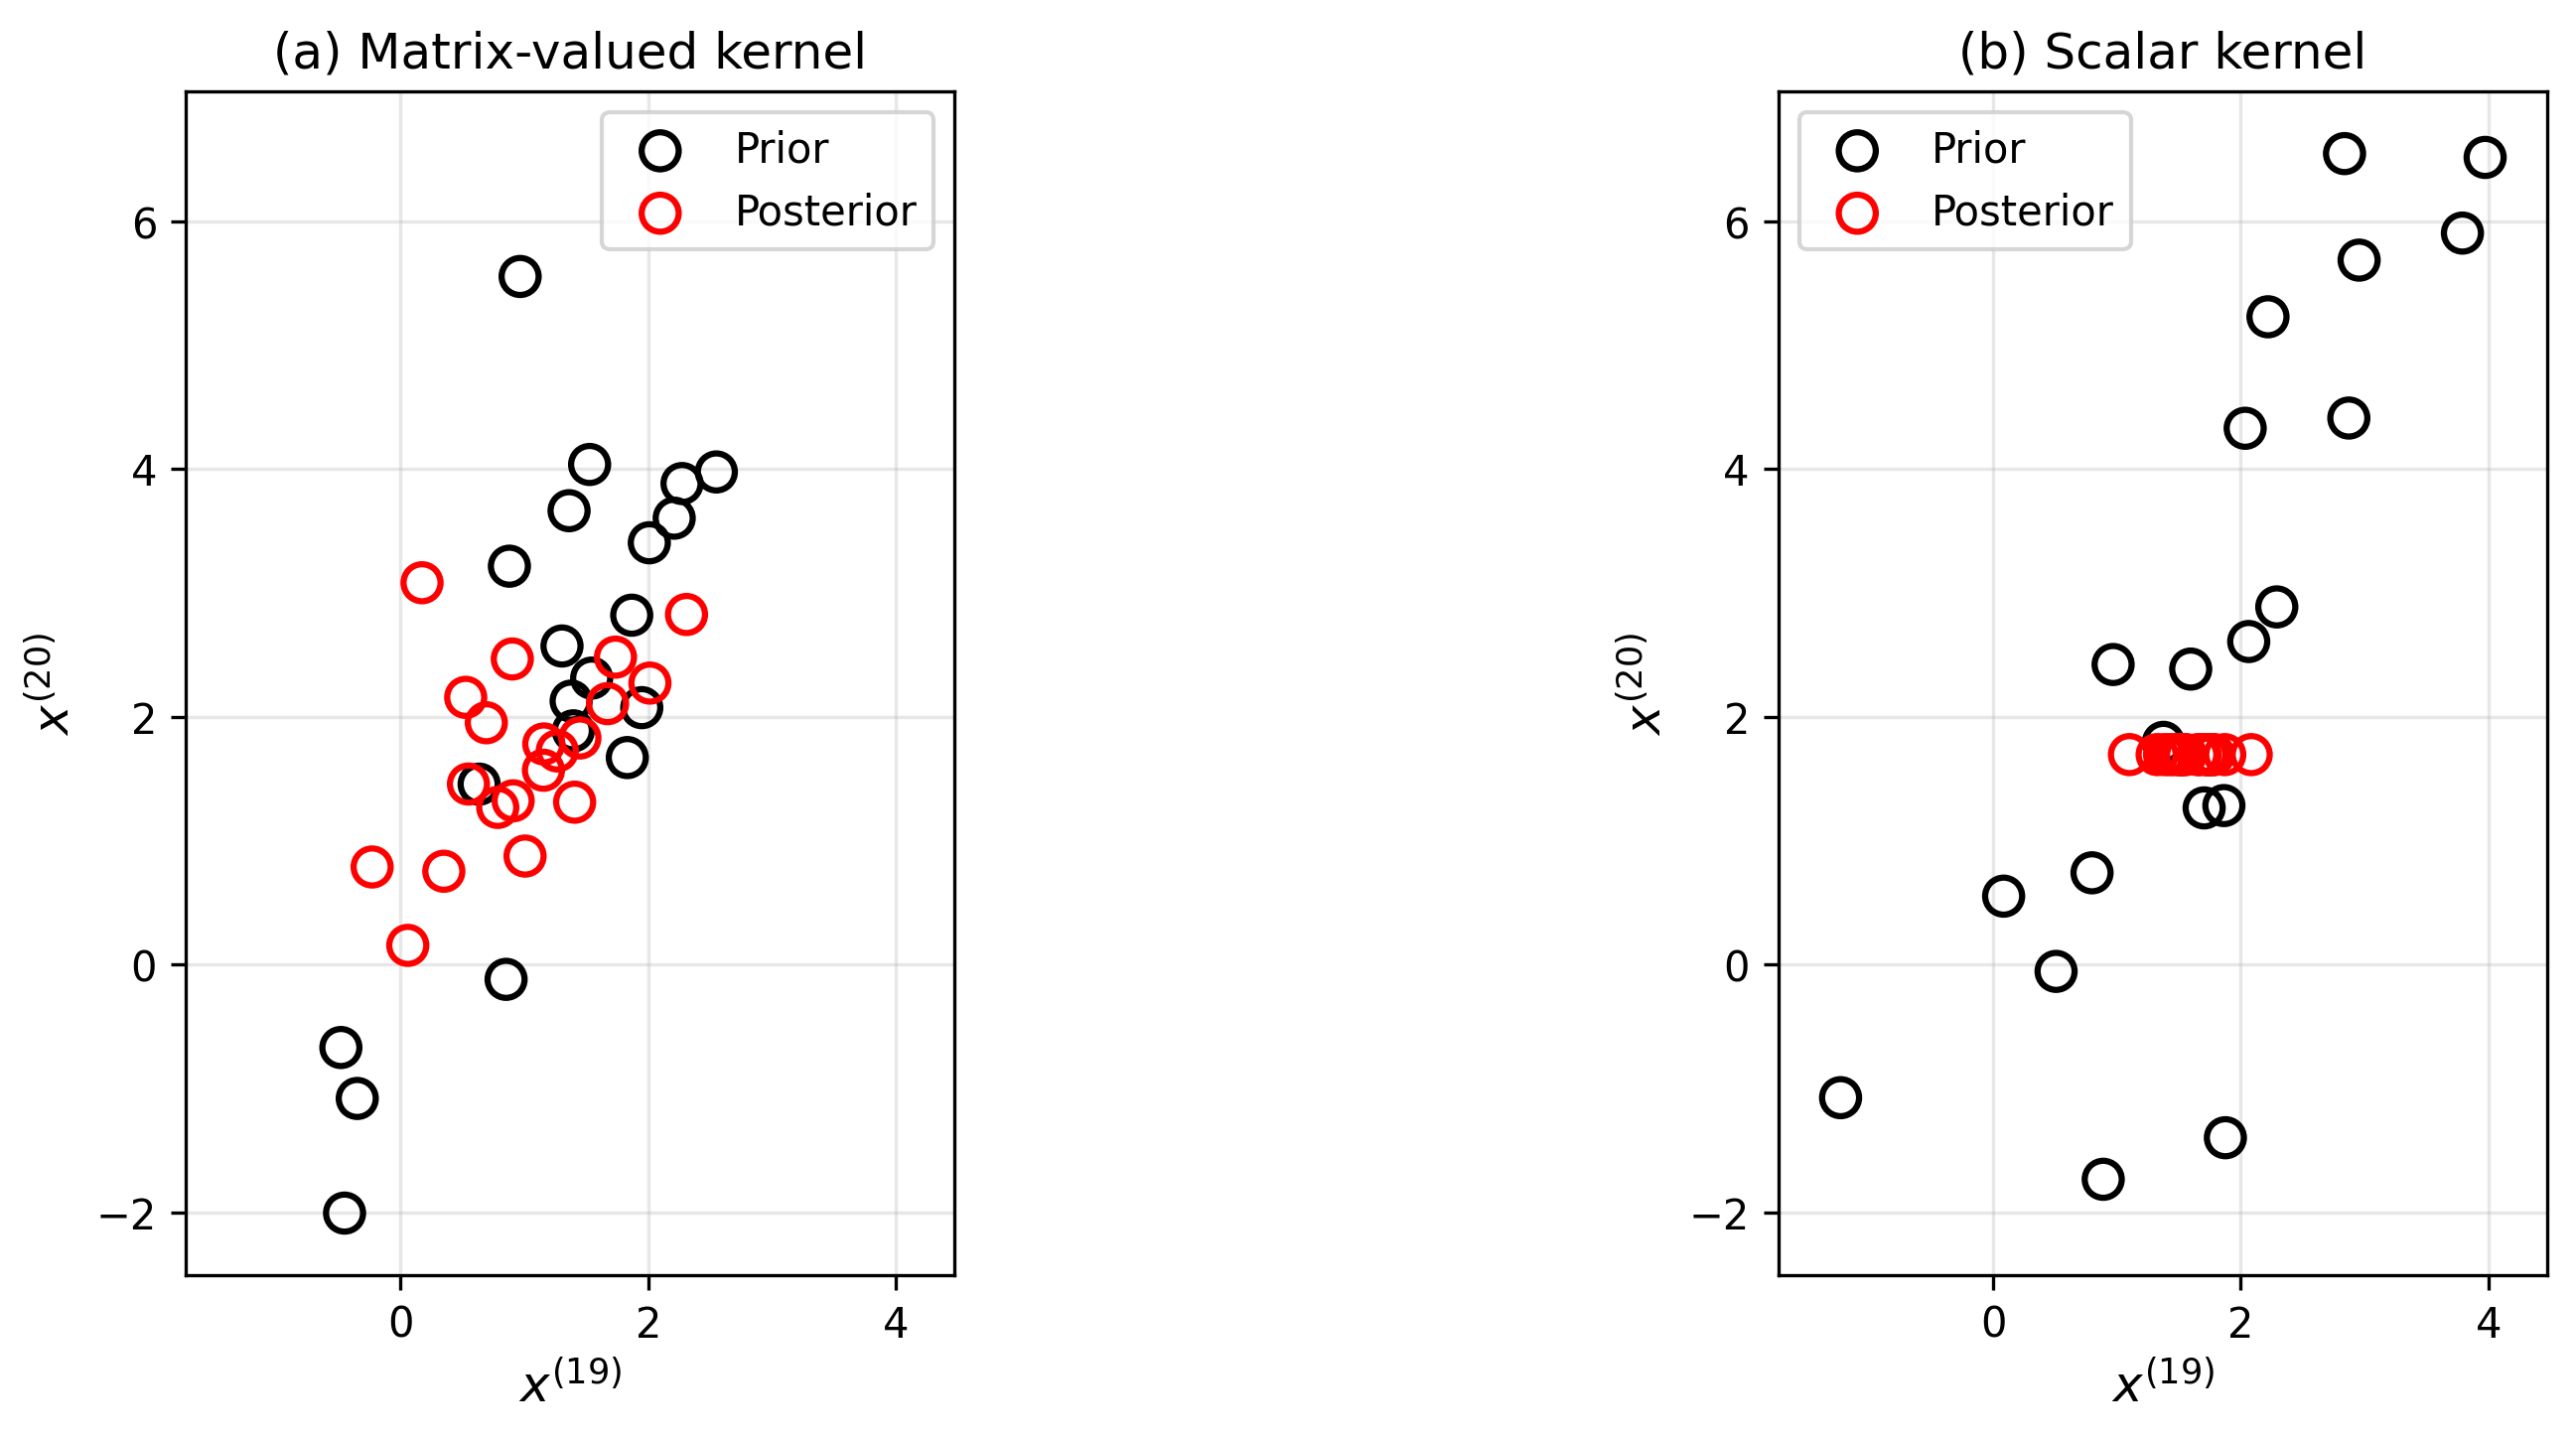
\includegraphics[width=0.5\linewidth]{figure3_reproduction.png}
    \caption{Switching to the matrix kernel prevents $x_{20}$ from collapsing to one point.}
    \label{fig:matrix_kernel}
\end{figure}

\subsubsection{Algorithm}

\begin{algorithm}[H]
\caption{Kernel Flow Filter --- Scalar Kernel}
\begin{algorithmic}[1]
\REQUIRE Particles $\{\mathbf{x}^{(i)}\}_{i=1}^{N}$ with equal weights, scalar bandwidth $\alpha = 1/N$
\REQUIRE Localization matrix $\mathbf{C}$ (Schur product mask), pseudo-time steps $n_s$, step size $\Delta t$
\FOR{$k = 1, 2, \ldots, T$}
  \STATE \textbf{Predict:} $\mathbf{x}_0^{(i)} \sim p(\mathbf{x}_k \mid \mathbf{x}^{(i)})$ for all $i$
  \STATE Compute ensemble mean $\bar{\mathbf{x}}_0$, localized covariance $\mathbf{B} = \mathbf{C} \circ \hat{\mathbf{P}}_{\text{sample}}$
  \STATE Precompute $\mathbf{B}^{-1}$, $\mathbf{R}^{-1}$, bandwidth $\sigma^2 = \alpha \cdot \text{tr}(\mathbf{B})/d$
  \FOR{$s = 1, \ldots, n_s$}
    \FOR{each particle $j$ (batched)}
      \STATE \textbf{Posterior gradient:}
      \STATE $\nabla \log p(\mathbf{z}_k \mid \mathbf{x}^{(j)}) = \mathbf{H}^{(j)\top}\mathbf{R}^{-1}(\mathbf{z}_k - \mathbf{h}(\mathbf{x}^{(j)}))$
      \STATE $\nabla \log p(\mathbf{x}^{(j)}) = -\mathbf{B}^{-1}(\mathbf{x}^{(j)} - \bar{\mathbf{x}}_0)$
      \STATE $\nabla \log \pi(\mathbf{x}^{(j)}) = \nabla \log p(\mathbf{z}_k \mid \mathbf{x}^{(j)}) + \nabla \log p(\mathbf{x}^{(j)})$
      \STATE \textbf{Scalar kernel:} $K(\mathbf{x}^{(i)}, \mathbf{x}^{(j)}) = \exp\!\left(-\frac{\|\mathbf{x}^{(i)}-\mathbf{x}^{(j)}\|^2}{2\sigma^2}\right)$
      \STATE \textbf{Kernel gradient:} $\nabla_{\mathbf{x}^{(i)}} K = -\frac{1}{\sigma^2}(\mathbf{x}^{(i)}-\mathbf{x}^{(j)}) K(\mathbf{x}^{(i)}, \mathbf{x}^{(j)})$
      \STATE \textbf{Flow:} $\mathbf{v}^{(j)} = \frac{1}{N}\sum_{i=1}^{N}\left[K(\mathbf{x}^{(i)}, \mathbf{x}^{(j)})\nabla \log\pi(\mathbf{x}^{(i)}) + \nabla_{\mathbf{x}^{(i)}}K(\mathbf{x}^{(i)}, \mathbf{x}^{(j)})\right]$
    \ENDFOR
    \STATE Precondition: $\mathbf{v}^{(j)} \leftarrow \mathbf{B}\, \mathbf{v}^{(j)}$
    \STATE $\mathbf{x}^{(j)} \leftarrow \mathbf{x}^{(j)} + \Delta t \cdot \mathbf{v}^{(j)}$ for all $j$
  \ENDFOR
\ENDFOR
\end{algorithmic}
\end{algorithm}

\begin{algorithm}[H]
\caption{Kernel Flow Filter --- Matrix (Tensor) Kernel}
\begin{algorithmic}[1]
\REQUIRE Same setup as scalar kernel. Per-dimension bandwidth: $(\sigma^{(d)})^2 = \alpha \cdot B_{dd}$
\FOR{$k = 1, 2, \ldots, T$}
  \STATE Predict and compute $\bar{\mathbf{x}}_0, \mathbf{B}, \mathbf{B}^{-1}, \mathbf{R}^{-1}$ as in scalar kernel
  \FOR{$s = 1, \ldots, n_s$}
    \FOR{each particle $j$ (batched)}
      \STATE Compute $\nabla \log \pi(\mathbf{x}^{(j)})$ as before
      \STATE \textbf{Matrix kernel} (diagonal, per-dimension):
      \STATE $K^{(d)}(\mathbf{x}^{(i)}, \mathbf{x}^{(j)}) = \exp\!\left(-\frac{(x_d^{(i)}-x_d^{(j)})^2}{2\alpha (\sigma^{(d)})^2}\right)$ for each dimension $d$
      \STATE $[\nabla_{\mathbf{x}^{(i)}} \cdot \mathbf{K}]^{(d)} = -\frac{x_d^{(i)}-x_d^{(j)}}{\alpha (\sigma^{(d)})^2} K^{(d)}(\mathbf{x}^{(i)}, \mathbf{x}^{(j)})$
      \STATE \textbf{Per-dimension flow:}
      \STATE $v_d^{(j)} = \frac{1}{N}\sum_{i=1}^{N}\left[K^{(d)}(\mathbf{x}^{(i)}, \mathbf{x}^{(j)})[\nabla \log\pi(\mathbf{x}^{(i)})]_d + [\nabla_{\mathbf{x}^{(i)}} \cdot \mathbf{K}]^{(d)}\right]$
    \ENDFOR
    \STATE Precondition: $\mathbf{v}^{(j)} \leftarrow \mathbf{B}\, \mathbf{v}^{(j)}$
    \STATE $\mathbf{x}^{(j)} \leftarrow \mathbf{x}^{(j)} + \Delta t \cdot \mathbf{v}^{(j)}$ for all $j$
  \ENDFOR
\ENDFOR
\end{algorithmic}
\end{algorithm}

\paragraph{Empirical takeaway (§4.6).} The matrix-valued kernel prevents the state-dimension collapse shown in Figure~\ref{fig:matrix_kernel}, which is the whole reason to use this filter. The use case is niche but concrete: a low-dimensional, well-conditioned target where the particle budget is severely constrained (on the order of $N \sim 20$) and the user is willing to pay the $O(N^2)$ kernel-matrix cost in exchange for keeping the small ensemble from collapsing.

\newpage

%%%%%%%%%%%%%%%%%%%%%%%%%%%%%%%%%%%%%%%%%%%%%%%%%%%%%%%%%%
\newpage
\section{Resampling and Optimal Transport}

\subsection{Two Problems with Resampling}

OT resampling's value in this report is \emph{differentiability}, not lower filtering RMSE. Table~\ref{tab:soft-vs-ot-sv} in \S\ref{par:soft-vs-ot} shows OT paying a $20$--$180\times$ compute tax depending on baseline and $\epsilon$, typically $60$--$100\times$ in HMC-relevant settings, without beating stop-gradient systematic or soft resampling on RMSE. The reason to pay that cost appears in \S\ref{sec:param-estimation}, where the gradient surface determines whether HMC can recover the parameter posterior.

Particle filters already showed the sample-impoverishment problem caused by low-quality resampling. The resampler should change the particle representation without changing the distribution it represents. Reich's OT resampler does this by treating resampling as a transport problem \cite{reich2013nonparametric}. Before resampling I have particle locations and weights $\{\omega_i, x_i\}$; after resampling I want $\{\tilde\omega_i, \tilde x_i\}$ with equal weights. Thinking of the locations as basis vectors and the weights as coefficients turns resampling into a linear transformation problem. The transformation builds an equal-weight approximation that reduces resampling variance and better preserves the structure of the distribution.

The target is simple: $\{\omega_i, x_i\}$ and $\{\tilde\omega_i, \tilde x_i\}$ should represent the same distribution, with $\tilde\omega_i \equiv \frac1N$ for $N$ particles. There are two resampling problems to separate.

\paragraph{Problem 1: Sampling noise.} OT resampling is deterministic. It avoids the extra sampling noise introduced by systematic resampling and improves covariance estimation from the particle cloud. Classical OT still requires solving a discrete linear program to find the optimal transport plan. Linear-program solvers only need the cost matrix and the marginal constraints. They do not provide derivatives of the optimal plan with respect to the inputs. That creates the second problem.

\paragraph{Problem 2: Non-differentiability.} The LP-based OT plan is not differentiable with respect to the inputs. For my purpose---building a differentiable particle filter whose log-likelihood can be differentiated with respect to model parameters---this is a showstopper. Entropy regularization fixes the mathematical object I need \cite{corenflos-differentiable-2021}: the optimal coupling $P^*$ becomes differentiable as a function of the cost matrix. The regularized transport cost is
\begin{equation}
    W_{2, \epsilon}^2 (\alpha_N, \beta_N) = \min_{P \in S(a, b)} \sum_{i,j=1}^N p_{i,j} \left( c_{i,j} + \epsilon \log \frac{p_{i,j}}{a_i b_j} \right)
\end{equation}
The practical issue is computing the gradient faithfully through the iterative Sinkhorn solver that finds $P^*$. The regularized OT map is differentiable in principle, but the backward pass still needs care. That is the focus for the rest of this section.

By adding the entropy term $\epsilon \log \frac{p_{i,j}}{a_i b_j}$ instead of $\epsilon \log p_{i,j}$, the authors of \cite{corenflos-differentiable-2021} made it possible to recover the transport plan from the dual variables alone. This objective is the entropic optimal transport problem, equivalent up to constants under fixed marginals to $\langle \mathbf{C}, \mathbf{P}\rangle - \epsilon \mathbf{H}(\mathbf{P})$. The dual recovery step is $\mathcal{O}(N)$ per entry, compared to $\mathcal{O}(N^2)$ for the primal LP of \cite{reich2013nonparametric}, which opens the possibility for modeling more complicated systems with large numbers of particles.
\subsection{Soft Resampling}

Soft resampling \cite{karkus2018particle} is a compromise between fully stochastic systematic resampling and fully deterministic OT resampling. The idea is to blend the particle weights with a uniform distribution before selection, then apply an importance correction after. The algorithm is given below.

\begin{algorithm}[H]
\caption{Soft Resampling}
\begin{algorithmic}[1]
\REQUIRE Particles $\{\mathbf{x}^{(i)}, w^{(i)}\}_{i=1}^N$ (weights normalized: $\sum_i w^{(i)}=1$)
\REQUIRE Trade-off parameter $\alpha \in [0,1]$ ($\alpha=1$: hard resampling, $\alpha=0$: pure importance sampling)
\STATE \textbf{Mixture distribution:}
\STATE $q^{(i)} \leftarrow \alpha\, w^{(i)} + (1-\alpha)/N$ for $i=1,\ldots,N$ \hfill ($q$ is strictly positive)
\STATE \textbf{Systematic sampling from $q$:}
\STATE Draw $u \sim \mathcal{U}[0, 1/N]$
\STATE $u^{(i)} \leftarrow u + (i-1)/N$ for $i=1,\ldots,N$
\STATE Select indices $j_i$ via cumulative sum of $q$: $\sum_{m=1}^{j_i-1} q^{(m)} < u^{(i)} \leq \sum_{m=1}^{j_i} q^{(m)}$
\STATE $\tilde{\mathbf{x}}^{(i)} \leftarrow \mathbf{x}^{(j_i)}$ for $i=1,\ldots,N$
\STATE \textbf{Importance weight correction:}
\STATE $\tilde{w}^{(i)} \leftarrow w^{(j_i)} / q^{(j_i)}$ for $i=1,\ldots,N$
\STATE $\tilde{w}^{(i)} \leftarrow \tilde{w}^{(i)} / \sum_j \tilde{w}^{(j)}$ \hfill (normalize)
\RETURN $\{\tilde{\mathbf{x}}^{(i)}, \tilde{w}^{(i)}\}_{i=1}^N$
\end{algorithmic}
\end{algorithm}

The critical observation is that soft resampling is only \emph{partially} differentiable. The selection step (line 6) is still discrete---the cumulative-sum lookup picks an integer index $j_i$, and the gradient does not flow through that choice. Only the importance weight correction $w^{(j_i)} / q^{(j_i)}$ on line 9 is differentiable through $w$. The selection gradient---how $\v\theta$ affects \emph{which} particle gets picked---is still zero. Section~\ref{sec:ot-derivative-chain} makes this precise.

\subsection{Entropy-Regularized OT (Sinkhorn) Resampling}
\label{sec:entropic-ot}

The entropy-regularized OT resampling problem is a direct application of the Monge-Kantorovich framework. To set up the problem, recall that in the Monge-Kantorovich problem we have two probability vectors $\mathbf{a} \in \mathbb{R}^N_+$ and $\mathbf{b} \in \mathbb{R}^N_+$ and a cost matrix $\mathbf{C} \in \mathbb{R}^{N\times N}$. The goal is to find the optimal coupling matrix $\mathbf{P} \in \mathbb{R}_+^{N\times N}$, where $P_{ij}$ describes the flow of mass from bin $i$ to bin $j$, minimizing total transport cost:
\begin{equation}
    \min_{\mathbf{P} \in \mathcal{U}(\mathbf{a}, \mathbf{b})} \langle \mathbf{C}, \mathbf{P} \rangle, \qquad
    \mathcal{U}(\mathbf{a}, \mathbf{b}) = \left\{ \mathbf{P} \in \mathbb{R}_+^{N\times N} : \mathbf{P}\mathbf{1}_N = \mathbf{a},\; \mathbf{P}^\top \mathbf{1}_N = \mathbf{b} \right\}.
\end{equation}
In the resampling context, set $\mathbf{a} = \mathbf{w}$ (particle weights as the source marginal), $\mathbf{b} = \frac{1}{N}\mathbf{1}_N$ (the uniform distribution as the target marginal), and $C_{ij} = \|\tilde{\mathbf{x}}^{(i)} - \tilde{\mathbf{x}}^{(j)}\|^2/2$ as the squared-distance cost between normalized particle positions. Solving this exactly via linear programming is computationally expensive and, more importantly, non-differentiable with respect to the inputs.

\paragraph{Convention used in the algorithm below.} With the marginals as above, the optimal coupling $\mathbf{P}^*$ has row sums $\mathbf{w}$ (source) and column sums $\tfrac{1}{N}\mathbf{1}_N$ (target). The resampled particles, following Reich~\cite{reich2013nonparametric}, are $\hat{\mathbf{x}}^{(i)} = (1/b_i)\sum_j P^*_{ji}\,\mathbf{x}^{(j)} = N\sum_j P^*_{ji}\,\mathbf{x}^{(j)}$, so each new particle is a convex combination of the old ones with column-wise weights of $\mathbf{P}^*$. I use a resampling matrix $T$ below such that $\hat{\mathbf{x}}^{(i)} = \sum_j T_{ij}\mathbf{x}^{(j)}$, which means $T_{ij} = N\,P^*_{ji}$. Thus $T$ is $N$ times the \emph{transpose} of the coupling $\mathbf{P}^*$. The normalization-and-weighting step in the OT resampling algorithm below converts $\mathbf{P}^*$ into this $T$. I state the convention because row-vs-column and source-vs-target are easy to swap silently when translating between the Reich formula and the Sinkhorn output.

The key insight from \cite{Cuturi2013SinkhornDL} is that adding a discrete entropy regularizer to the objective,
\begin{equation}
    \min_{\mathbf{P} \in \mathcal{U}(\mathbf{a}, \mathbf{b})} \langle \mathbf{C}, \mathbf{P} \rangle - \epsilon\, \mathbf{H}(\mathbf{P}), \qquad \mathbf{H}(\mathbf{P}) = -\sum_{i,j} P_{ij}(\log P_{ij} - 1),
\end{equation}
makes the problem $\epsilon$-strongly convex, yielding a unique solution that is differentiable with respect to $\mathbf{a}$, $\mathbf{b}$, and $\mathbf{C}$. By the KKT conditions, the optimal $\mathbf{P}^*$ must have the Gibbs-kernel form:
\begin{equation}
    P_{ij}^* = u_i\, K_{ij}\, v_j, \qquad K_{ij} = \exp\!\left(-\frac{C_{ij}}{\epsilon}\right),
    \label{eq:gibbs-kernel}
\end{equation}
where $\mathbf{u} \in \mathbb{R}^N$ and $\mathbf{v} \in \mathbb{R}^N$ are two unknown scaling vectors. To determine them, substitute this form back into the two marginal constraints $\mathbf{P}^*\mathbf{1}_N = \mathbf{a}$ and $(\mathbf{P}^*)^\top \mathbf{1}_N = \mathbf{b}$, obtaining the equivalent fixed-point conditions:
\begin{equation}
    \mathbf{u} \odot (\mathbf{K}\mathbf{v}) = \mathbf{a}, \qquad \mathbf{v} \odot (\mathbf{K}^\top \mathbf{u}) = \mathbf{b},
\end{equation}
where $\odot$ and $\oslash$ denote element-wise multiplication and division. Rearranging gives alternating updates for $\mathbf{u}$ and $\mathbf{v}$:
\begin{equation}
    \mathbf{u}^{(\ell)} = \mathbf{a} \oslash \!\left(\mathbf{K}\mathbf{v}^{(\ell-1)}\right), \qquad \mathbf{v}^{(\ell)} = \mathbf{b} \oslash \!\left(\mathbf{K}^\top \mathbf{u}^{(\ell)}\right),
    \label{eq:vanilla-sinkhorn}
\end{equation}
initialized at $\mathbf{v}^{(0)} = \mathbf{1}_N$. Upon convergence, the optimal coupling is recovered as $\mathbf{P}^{(L)} = \mathrm{diag}(\mathbf{u}^{(L)}) \cdot \mathbf{K} \cdot \mathrm{diag}(\mathbf{v}^{(L)})$. This is the vanilla Sinkhorn algorithm.

The practical difficulty is numerical: since $K_{ij} = \exp(-C_{ij}/\epsilon)$, when particle positions are spread out or $\epsilon$ is small, the entries of $\mathbf{K}$ become extremely small, and the repeated divisions in \eqref{eq:vanilla-sinkhorn} cause the scaling variables $\mathbf{u}$ and $\mathbf{v}$ to grow in the exponential domain, producing infinite or non-finite values. This is the well-known numeric instability of the vanilla Sinkhorn. The standard remedy is to absorb the scaling into dual potentials $\boldsymbol{\alpha} = \epsilon \log \mathbf{u}$ and $\boldsymbol{\beta} = \epsilon \log \mathbf{v}$, so that the coupling takes the form
\begin{equation}
    T_{ij} = \exp\!\left(\frac{\alpha_i + \beta_j - C_{ij}}{\epsilon}\right),
\end{equation}
and the marginal-matching updates \eqref{eq:vanilla-sinkhorn} turn into log-sum-exp operations. These can be stabilized numerically by subtracting the row or column minimum before exponentiating --- this is the log-stabilized Sinkhorn, whose iteration is given in the algorithm below.

\begin{algorithm}[H]
\caption{Sinkhorn Iteration (Dual Potentials)}
\begin{algorithmic}[1]
\REQUIRE Cost matrix $\mathbf{C} \in \mathbb{R}^{N\times N}$, $C_{ij} = \|\mathbf{x}^{(i)}-\mathbf{x}^{(j)}\|^2/2$
\REQUIRE Log-weights $\log w^{(i)}$, regularization $\epsilon > 0$, max iterations, threshold $\delta$
\STATE Initialize dual potentials: $\alpha^{(i)} \leftarrow 0$, $\beta^{(i)} \leftarrow 0$ for $i=1,\ldots,N$
\STATE $\log u \leftarrow -\log N$ \hfill (uniform target: $1/N$)
\REPEAT
  \STATE $\alpha_{\text{new}}^{(i)} \leftarrow -\epsilon \log\sum_j \exp\!\left(\frac{\log w^{(j)} + \beta^{(j)}/\epsilon - C_{ji}/\epsilon}{1}\right)$ \hfill (softmin over columns)
  \STATE $\beta_{\text{new}}^{(j)} \leftarrow -\epsilon \log\sum_i \exp\!\left(\frac{\log u + \alpha_{\text{new}}^{(i)}/\epsilon - C_{ij}/\epsilon}{1}\right)$ \hfill (softmin over rows)
  \STATE $\boldsymbol{\alpha} \leftarrow \tfrac{1}{2}(\boldsymbol{\alpha} + \boldsymbol{\alpha}_{\text{new}})$, \quad $\boldsymbol{\beta} \leftarrow \tfrac{1}{2}(\boldsymbol{\beta} + \boldsymbol{\beta}_{\text{new}})$ \hfill (damping for stability)
\UNTIL{$\max(|\Delta\boldsymbol{\alpha}|, |\Delta\boldsymbol{\beta}|) < \delta$ or max iterations reached}
\STATE \textbf{Single-step extrapolation} (approximate automatic-differentiation window; \emph{not} the implicit function theorem route --- see \S\ref{sec:sinkhorn-backward}):
\STATE $\boldsymbol{\alpha}_{\text{det}} \leftarrow \operatorname{detach}(\boldsymbol{\alpha})$, $\boldsymbol{\beta}_{\text{det}} \leftarrow \operatorname{detach}(\boldsymbol{\beta})$
\STATE One more Gauss-Seidel step: $\boldsymbol{\alpha} \leftarrow \text{softmin}(\epsilon, \mathbf{C}^\top, \log\mathbf{w} + \boldsymbol{\beta}_{\text{det}}/\epsilon)$
\STATE $\boldsymbol{\beta} \leftarrow \text{softmin}(\epsilon, \mathbf{C}, \log\mathbf{u} + \boldsymbol{\alpha}/\epsilon)$
\RETURN $\boldsymbol{\alpha}, \boldsymbol{\beta}$
\end{algorithmic}
\end{algorithm}

Lines 9--11 of the algorithm above are the \emph{extrapolation trick} for approximate differentiability. The converged potentials $(\boldsymbol{\alpha}, \boldsymbol{\beta})$ are detached from the derivative graph, and one additional Gauss--Seidel step is taken on the live graph. This gives automatic differentiation a single-step window into how the potentials depend on the inputs $(\mathbf{C}, \log\mathbf{w})$, without differentiating through all the preceding iterations. Section~\ref{sec:sinkhorn-backward} shows why this is only an approximation---accurate for weight gradients but biased for particle-position gradients---and why implicit differentiation is the correct alternative.

\begin{algorithm}[H]
\caption{Entropy-Regularized Optimal Transport Resampling}
\begin{algorithmic}[1]
\REQUIRE Particles $\{\mathbf{x}^{(i)}, w^{(i)}\}_{i=1}^N$, regularization $\epsilon$
\STATE \textbf{Normalize particles:} $\tilde{\mathbf{x}}^{(i)} \leftarrow (\mathbf{x}^{(i)} - \bar{\mathbf{x}}) / s$ where $\bar{\mathbf{x}} = \text{mean}$, $s = \text{std}\cdot\sqrt{d}$
\STATE Compute cost matrix: $C_{ij} = \|\tilde{\mathbf{x}}^{(i)} - \tilde{\mathbf{x}}^{(j)}\|^2 / 2$
\STATE Solve dual potentials: $(\boldsymbol{\alpha}, \boldsymbol{\beta}) \leftarrow \text{Sinkhorn}(\log\mathbf{w}, \mathbf{C}, \epsilon)$
\STATE \textbf{Transport matrix:}
\STATE $\log T_{ij} \leftarrow (\alpha_i + \beta_j - C_{ij})/\epsilon$
\STATE Normalize columns: $T_{ij} \leftarrow T_{ij} / \sum_k T_{kj}$ \hfill (each column sums to $1/N$)
\STATE Apply source weights: $T_{ij} \leftarrow T_{ij} \cdot w^{(j)}$ \hfill (rows marginalize to $\mathbf{w}$)
\STATE \textbf{Transport particles:}
\STATE $\hat{\mathbf{x}}^{(i)} \leftarrow \sum_j T_{ij}\, \mathbf{x}^{(j)}$ \hfill (matrix-vector product)
\STATE $\hat{w}^{(i)} \leftarrow 1/N$ for all $i$ \hfill (uniform weights after transport)
\RETURN $\{\hat{\mathbf{x}}^{(i)}, \hat{w}^{(i)}\}_{i=1}^N$, transport matrix $\mathbf{T}$
\end{algorithmic}
\end{algorithm}

\paragraph{Consistency: why the output is a realisation of $q$.}
The Sinkhorn solver itself is agnostic to what either marginal represents --- give it any $\mathbf{a}$ and $\mathbf{b}$ on any support and it returns the entropy-regularised OT plan between them. Nothing in the algorithm references a continuous distribution. The reason the resampled cloud $\{(\hat{\mathbf{x}}^{(i)}, 1/N)\}$ is asymptotically a realisation of the underlying target $q$ is a consistency theorem due to Reich \cite{reich2013nonparametric}.

\textbf{Theorem (Reich, ETPF consistency).} Let $q$ be a probability density on $\mathbb{R}^d$. Suppose particles $\mathbf{x}^{(1)}, \ldots, \mathbf{x}^{(N)}$ are drawn i.i.d.\ from a proposal $q_{\text{prop}}$ absolutely continuous w.r.t.\ Lebesgue, with importance weights $w^{(i)} \propto q(\mathbf{x}^{(i)}) / q_{\text{prop}}(\mathbf{x}^{(i)})$ normalised to $\sum_i w^{(i)} = 1$. Let $\mathbf{P}^{*}$ be the unregularised OT plan with marginals $(\mathbf{w}, \tfrac{1}{N}\mathbf{1})$ on the support $\{\mathbf{x}^{(i)}\}$ and L\textsuperscript{2} cost $C_{ij} = \|\mathbf{x}^{(i)} - \mathbf{x}^{(j)}\|^2$. Define the barycentric output $\hat{\mathbf{x}}^{(i)} = N \sum_j P^{*}_{ji}\, \mathbf{x}^{(j)}$. Then under standard regularity (weights uniformly bounded in $N$; $q, q_{\text{prop}}$ admit a unique Brenier transport map under L\textsuperscript{2} cost), for every continuous bounded test function $f$,
\begin{equation}
\frac{1}{N}\sum_{i=1}^N f(\hat{\mathbf{x}}^{(i)}) \;\xrightarrow{N \to \infty}\; \int f \, dq \quad \text{a.s.},
\end{equation}
i.e.\ $\tfrac{1}{N}\sum_i \delta_{\hat{\mathbf{x}}^{(i)}}$ converges weakly to $q$.

\textit{Proof sketch.} The discrete plan $\mathbf{P}^{*}$ converges as $N \to \infty$ to the continuous Brenier map $T_{q_{\text{prop}}\to q}$ that pushes $q_{\text{prop}}$ onto $q$ under L\textsuperscript{2} cost. The barycentric projection $\hat{\mathbf{x}}^{(i)} = N \sum_j P^{*}_{ji}\, \mathbf{x}^{(j)}$ approximates $T_{q_{\text{prop}}\to q}(\mathbf{x}^{(i)})$ in the limit. Since the $\mathbf{x}^{(i)}$ are samples of $q_{\text{prop}}$, the images $\hat{\mathbf{x}}^{(i)}$ are asymptotically samples of $q$. The full argument is in \cite{reich2013nonparametric} Section~4.

\textit{Caveats.}
\begin{enumerate}
\item The theorem is stated for $\epsilon = 0$ (LP-OT). The entropy-regularised Sinkhorn version used in practice adds a bias of order $\epsilon$ that survives the $N \to \infty$ limit unless $\epsilon$ is also driven to zero. The standard schedule is $\epsilon = \epsilon(N) \to 0$ at a rate slow enough to preserve numerical stability.
\item Convergence is weak (test integrals), not in stronger metrics like total variation. Finite-$N$ rates suffer the curse of dimensionality: the Wasserstein-2 distance of the empirical from $q$ is $\mathcal{O}(N^{-1/d})$.
\item The L\textsuperscript{2} cost choice is load-bearing for Brenier --- other costs give different limit maps.
\end{enumerate}

This is the only place the underlying $q$ enters the OT-resampling pipeline. The Sinkhorn algorithm sees $\mathbf{a}, \mathbf{b}, \mathbf{C}$ and nothing else; the barycentric projection is what converts its plan into output positions; Reich's theorem is what guarantees those positions are asymptotically faithful to $q$.

\subsection{The Derivative Chain through Resampling}
\label{sec:ot-derivative-chain}

The core difficulty in differentiating through a particle filter is the resampling step. Everything else---the transition model $p(x_k \mid x_{k-1}, \v\theta)$, the observation likelihood $p(z_k \mid x_k, \v\theta)$, and the weight computation---is differentiable. Resampling is the step where discrete particle selection breaks the gradient flow. To understand what each method does and does not give, trace the derivative chain explicitly.

At time step $k$, the negative log-likelihood contribution is $-\log \sum_i \tilde{w}_k^{(i)}$ where the unnormalized weights $\tilde{w}_k^{(i)} = w_{k-1}^{(i)} \cdot p(z_k \mid x_k^{(i)}, \v\theta)$ depend on $\v\theta$ both through the observation model and through the particle positions $x_k^{(i)}$. Particle $x_k^{(i)}$ was sampled from $p(x_k \mid x_{k-1}^{(j_i)}, \v\theta)$, where $j_i$ is the index selected by resampling at step $k-1$. The derivative $\partial x_k^{(i)} / \partial \v\theta$ therefore has two contributions: the direct effect through the transition model (differentiable) and the indirect effect through which ancestor $j_i$ was selected (depends on how resampling is done).

\paragraph{Systematic resampling with stop gradient.}
Treat the selected particle indices as constants and detach the gradient at the resampling step. The derivative flows only through the weights after resampling and the transition model, but sees nothing about how $\v\theta$ affects particle selection. The gradient is:
\begin{equation}
    \frac{\partial L}{\partial \v\theta} = -\sum_k \sum_i \frac{\partial \log p(z_k \mid x_k^{(i)}, \v\theta)}{\partial \v\theta} + \frac{\partial \log p(x_k^{(i)} \mid x_{k-1}^{(j_i)}, \v\theta)}{\partial \v\theta}
\end{equation}
where $x_{k-1}^{(j_i)}$ is treated as a fixed constant. This \textit{selection gradient} is zero. The resulting gradient is biased---it misses the signal from particle selection---but bounded and continuous within each particle configuration. This makes it safe for both SGD and (in simple models) HMC.

\paragraph{Soft resampling.}
Soft resampling \cite{karkus2018particle} blends the weights with a uniform distribution before selection: $\tilde{w}_i = \alpha\, w_i + (1-\alpha)/N$. Particles are still selected discretely from $\tilde{w}_i$, but an importance correction weight $w_i / \tilde{w}_i$ is applied after selection and is differentiable with respect to $\v\theta$ through $w_i$. The gradient now flows through this correction factor in addition to the direct observation and transition terms. It does not flow through which particle was selected. Soft resampling is therefore partially differentiable---richer gradient information than stop gradient, but the selection is still invisible.

\paragraph{OT resampling.}
Optimal transport resampling \cite{corenflos-differentiable-2021} replaces discrete index selection entirely with a continuous transport map. With the transport matrix $T$ from the Sinkhorn algorithm, the resampled particles are the weighted average:
\begin{equation}
    \tilde{x}_k^{(i)} = \sum_j T_{ij}\, x_k^{(j)}.
\end{equation}
There is no discrete selection---every input particle contributes to every output particle through $T_{ij}$. The key point is that $T$ is itself a function of both the particle positions $\mathbf{x}_k$ (through the cost matrix $C_{ij} = \|\tilde x^{(i)} - \tilde x^{(j)}\|^2/2$) and the weights $\mathbf{w}_k$ (through the Sinkhorn marginal constraints). The total derivative of the resampled particles with respect to $\v\theta$ therefore has three terms, written schematically as:
\begin{equation}
    \frac{d\tilde{\mathbf{x}}_k}{d\v\theta} = \underbrace{\frac{\partial T}{\partial \mathbf{x}_k} \frac{d\mathbf{x}_k}{d\v\theta} \cdot \mathbf{x}_k}_{\text{Term 1: particle geometry}} + \underbrace{T \cdot \frac{d\mathbf{x}_k}{d\v\theta}}_{\text{Term 2: direct transport}} + \underbrace{\frac{\partial T}{\partial \mathbf{w}_k} \frac{d\mathbf{w}_k}{d\v\theta} \cdot \mathbf{x}_k}_{\text{Term 3: weight gradient}}
    \label{eq:ot-three-terms}
\end{equation}
with the symbols defined as follows: $\v\theta \in \mathbb{R}^{d_\theta}$ is the model-parameter vector being estimated (the object HMC later samples in \S\ref{sec:param-estimation}); $\mathbf{x}_k = (x_k^{(1)}, \ldots, x_k^{(N)}) \in \mathbb{R}^{N \times d_x}$ is the stacked pre-resampling particle cloud at time $k$ with $N$ particles in $d_x$-dimensional state space; $\mathbf{w}_k = (w_k^{(1)}, \ldots, w_k^{(N)}) \in \mathbb{R}^{N}$ is the normalized importance-weight vector; $\tilde{\mathbf{x}}_k = (\tilde x_k^{(1)}, \ldots, \tilde x_k^{(N)}) \in \mathbb{R}^{N \times d_x}$ is the stacked post-resampling cloud produced by the transport map $\tilde x_k^{(i)} = \sum_j T_{ij}\, x_k^{(j)}$; $T \in \mathbb{R}^{N \times N}$ is the transport matrix returned by the Sinkhorn solver; $C \in \mathbb{R}^{N \times N}$ is the squared-distance cost matrix that feeds the Sinkhorn iteration; and the derivatives $d\mathbf{x}_k / d\v\theta$ and $d\mathbf{w}_k / d\v\theta$ are total derivatives that already account for the dependence of time-$k$ quantities on $\v\theta$ via the filter recursion up to step $k$. This is a schematic chain rule---the object $\partial T / \partial \mathbf{x}_k$ is a higher-order tensor and the contractions are suppressed for clarity. The three paths are:
\begin{itemize}
    \item \textbf{Term 1 (particle geometry):} A change in $\v\theta$ changes particle positions, which changes the cost matrix $C$, which changes the Sinkhorn potentials, which changes $T$, which changes the transported particles.
    \item \textbf{Term 2 (direct transport):} A change in $\v\theta$ changes particle positions, which are directly transported by the (fixed) transport matrix $T$.
    \item \textbf{Term 3 (weight gradient):} A change in $\v\theta$ changes the observation likelihood, which changes the weights, which changes $T$, which changes the transported particles. This is the \emph{selection gradient} that stop-gradient and soft resampling miss entirely.
\end{itemize}
Together, these three paths give a gradient that is correct in principle. The regularized OT map is smooth, so the loss surface is continuous. The practical issue is computing this gradient faithfully through the iterative Sinkhorn solver. Section~\ref{sec:sinkhorn-backward} addresses that problem.

A summary of the gradient properties of each method is given in Table~\ref{tab:resampling_grad}.

\begin{table}[H]
\centering
\caption{Resampling strategies for differentiable particle filters.}
\label{tab:resampling_grad}
\begin{tabular}{lcccc}
\toprule
Resampling & Fully diff.? & Selection gradient & Gradient bounded? & Loss continuous? \\
\midrule
Systematic (stop grad) & No  & None    & Yes               & No  \\
Soft                   & Partial & Partial & Yes            & No  \\
OT Sinkhorn            & In principle & Full    & Yes\textsuperscript{\textdagger} & Yes\textsuperscript{\textdagger} \\
\bottomrule
\end{tabular}
\vspace{2pt}
{\footnotesize \textsuperscript{\textdagger}For OT Sinkhorn, gradient boundedness and loss continuity hold under a fixed conditional-resampling branch and a well-conditioned Sinkhorn solve. They are not unconditional guarantees.}
\end{table}

\paragraph{Implications for HMC.}
HMC's leapfrog integrator treats the gradient as a deterministic force field. Two properties are critical: the gradient must be bounded (a single spike can send the trajectory to infinity and waste the proposal) and the loss surface must be continuous (discontinuities in $U(\v\theta)$ cause large $\Delta H$ and rejected proposals). Systematic resampling satisfies the first but not the second, because small changes in $\v\theta$ can flip a particle across a resampling threshold, causing a jump in the log-likelihood. OT resampling satisfies both: the transport map is smooth, so the loss surface is continuous, and there is no threshold discontinuity. There is a subtlety: even with OT resampling, conditional resampling (triggered when ESS drops below a threshold) introduces a second source of non-smoothness---the branch between ``resample'' and ``don't resample'' is itself a discontinuity. OT makes this much less severe because the ESS stays closer to $N$ when transport is smooth, but it does not eliminate it entirely. For simple models where the loss surface is already mild (e.g., linear Gaussian), systematic resampling can work fine with HMC. For nonlinear models with strong particle diversity effects, OT resampling is the right choice.


\paragraph{Empirical check: soft vs.\ OT resampling on stochastic volatility.}
\label{par:soft-vs-ot}
The theoretical picture above says OT resampling should give fuller gradients than soft or stop-gradient systematic, at the cost of extra compute. Table~\ref{tab:soft-vs-ot-sv} puts numbers on that trade-off for a 1D stochastic volatility run ($T = 500$, $N = 200$).

\begin{table}[H]
\centering
\footnotesize
\caption{Resampling comparison on stochastic volatility (1D, $T=500$, $N=200$). Headline: OT adds roughly $20$--$180\times$ wall-time vs.\ systematic / soft depending on $\epsilon$, with the HMC-relevant settings typically around $60$--$100\times$, and gives no RMSE improvement. Soft resampling ties stop-gradient on RMSE at the same cost. Systematic is the cheapest and has the best RMSE of this group; OT's value is gradient quality under HMC (\S\ref{sec:param-estimation}), not filtering accuracy.}
\label{tab:soft-vs-ot-sv}
\begin{tabular}{llccccc}
\toprule
Method & Param & RMSE & Log-lik & Wall (s) & ms/step & Resample rate \\
\midrule
PF (systematic, stop-grad) & --- & $1.142$ & $-547.56$ & $2.12$  & $4.25$  & $0.358$ \\
\midrule
Soft & $\alpha = 0.5$ & $1.140$ & $-545.37$ & $2.32$  & $4.64$  & $0.532$ \\
Soft & $\alpha = 0.7$ & $1.137$ & $-544.05$ & $2.26$  & $4.52$  & $0.426$ \\
Soft & $\alpha = 0.9$ & $1.135$ & $-545.60$ & $2.26$  & $4.52$  & $0.370$ \\
\midrule
OT   & $\epsilon = 0.1$ & $1.582$ & $-702.84$ & $359.45$ & $718.91$ & $0.420$ \\
OT   & $\epsilon = 0.3$ & $1.560$ & $-839.05$ & $182.84$ & $365.68$ & $0.432$ \\
OT   & $\epsilon = 0.5$ & $1.841$ & $-703.65$ & $156.06$ & $312.12$ & $0.428$ \\
OT   & $\epsilon = 1.0$ & $2.110$ & $-723.65$ & $47.94$  & $95.89$  & $0.432$ \\
\bottomrule
\end{tabular}
\end{table}

Three observations. First, on filtering accuracy alone OT does not outperform --- it is $20$--$180\times$ slower depending on baseline and $\epsilon$, typically $60$--$100\times$ in HMC-relevant settings, with strictly worse RMSE on this model across every $\epsilon$. Second, increasing the Sinkhorn regularisation $\epsilon$ buys speed at the cost of further RMSE degradation, as expected: larger $\epsilon$ is a softer transport plan that under-corrects the weight information. Third, soft resampling matches stop-gradient systematic on RMSE at essentially the same cost --- no accuracy penalty, partial differentiability. The case for paying OT's compute tax is therefore not `better filter,' it is `better gradient surface for HMC.' That is tested in \S\ref{sec:param-estimation}.

\subsection{Approximate vs Implicit Sinkhorn Backward}
\label{sec:sinkhorn-backward}

The entropy-regularized OT map is differentiable in principle. The practical question is how to compute the backward pass through the Sinkhorn iteration. There are two approaches, and their difference matters for correct gradients in the differentiable particle filter pipeline.

\subsubsection{The Extrapolation Approximation}

The approximate approach described in the Sinkhorn algorithm above runs the iteration to convergence, detaches the converged potentials from the computation graph, and takes one more Gauss--Seidel step on the live graph:
\begin{align}
    \boldsymbol{\alpha}_{\mathrm{det}} &= \operatorname{detach}(\boldsymbol{\alpha}_{\mathrm{converged}}), \quad \boldsymbol{\beta}_{\mathrm{det}} = \operatorname{detach}(\boldsymbol{\beta}_{\mathrm{converged}}), \\
    \boldsymbol{\alpha}_{\mathrm{new}} &= \mathrm{softmin}\!\left(\epsilon,\, \mathbf{C}^\top,\, \log\mathbf{w} + \boldsymbol{\beta}_{\mathrm{det}}/\epsilon\right), \\
    \boldsymbol{\beta}_{\mathrm{new}} &= \mathrm{softmin}\!\left(\epsilon,\, \mathbf{C},\, \log\mathbf{u} + \boldsymbol{\alpha}_{\mathrm{new}}/\epsilon\right).
\end{align}
Automatic differentiation sees only this final step. The true derivative of the converged potentials with respect to the inputs $(\mathbf{C}, \log\mathbf{w})$ would require differentiating through all iterations. The one-step window is an approximation.

Recall the three-term chain-rule decomposition of $d\tilde{\mathbf{x}}_k/d\v\theta$ from Equation~\ref{eq:ot-three-terms}: \textbf{Term 1} is the particle-geometry gradient that flows through $\partial T/\partial \mathbf{x}_k$, \textbf{Term 2} is the direct-transport gradient $T \cdot d\mathbf{x}_k/d\v\theta$, and \textbf{Term 3} is the weight gradient that flows through $\partial T/\partial \mathbf{w}_k$. The single-step extrapolation above is accurate for \textbf{Term 3}, because the weights $\mathbf{w}_k$ enter linearly into the Sinkhorn marginal constraint and the one-step update captures their effect well. But it is biased for \textbf{Term 1}, because the particle positions $\mathbf{x}_k$ affect the cost matrix $C$ which feeds into \emph{every} Sinkhorn iteration, not just the last one, and the single-step window cannot capture how the potentials depend on $C$ across the full iteration history. Term 2 is unaffected by the Sinkhorn backward because it does not pass through $T$.

When does this matter? It depends on whether $d\mathbf{x}_k / d\v\theta$ is zero or not. For a Bootstrap Particle Filter (BPF) on a linear Gaussian model with $\v\theta = \sigma_{\mathrm{obs}}$, the particles come from the state transition $x_k^{(i)} = F \tilde{x}_{k-1}^{(i)} + B \epsilon_k^{(i)}$, which does not depend on $\v\theta$. So $d\mathbf{x}_k/d\v\theta = 0$, Terms 1 and 2 vanish, and only Term 3 survives. The extrapolation approximation works well: I observe an automatic-differentiation-to-numerical-derivative ratio of approximately $1.08$. For LEDH (Local Exact Daum--Huang), the flow matrices depend on $\v\theta$ through $R = \sigma_{\mathrm{obs}}^2 DD^\top$, so $d\mathbf{x}_k / d\v\theta \neq 0$ and all three terms are active. The extrapolation approximation produces a ratio of approximately $1.33$---a clear bias from Term 1. These ratios are empirical validation targets on a specific model, not universal constants, but they sharply illustrate the problem.

\subsubsection{Implicit Differentiation at the Fixed Point}

The proper fix is implicit differentiation. At convergence, the Sinkhorn potentials satisfy a system of fixed-point equations (the marginal constraints). By the implicit function theorem, I can compute the exact Jacobian of the converged potentials with respect to the inputs without differentiating through the iteration \cite{cremers2022unifiedframeworkimplicit}.

The idea is as follows. Let $\mathbf{f}$ and $\mathbf{g}$ denote the converged dual potentials (absorbing the log-scaling), and let $P_{ij} = \exp((f_i + g_j - C_{ij})/\epsilon)$ be the transport plan at the fixed point. Given an upstream gradient $\partial L / \partial T$, the vector-Jacobian product (VJP) needs $\partial L / \partial \mathbf{C}$ and $\partial L / \partial \log\mathbf{w}$. The implicit VJP reduces to solving a $(2N-1) \times (2N-1)$ linear system:
\begin{equation}
    \mathbf{B}\boldsymbol{\mu} = \mathbf{r},
\end{equation}
where $\mathbf{B}$ is formed from the transport plan $\mathbf{T}$ and the source/target marginals $\mathbf{a}$, $\mathbf{b}$:
\begin{equation}
    \mathbf{B} = \begin{pmatrix} \mathrm{diag}(\mathbf{a}_{1:N-1}) & T_{1:N-1,:} \\ T_{1:N-1,:}^\top & \mathrm{diag}(\mathbf{b}) \end{pmatrix} + \rho\, \mathbf{I},
\end{equation}
and $\mathbf{r}$ is the right-hand side constructed from the upstream gradient $\partial L / \partial T$. The system is rank-deficient by 1 because the potentials are defined up to a global constant (a gauge freedom), so one equation is dropped and a small ridge $\rho$ is added for numerical stability. Once $\boldsymbol{\mu}$ is solved, the gradient with respect to the cost matrix is
\begin{equation}
    \frac{\partial L}{\partial C_{ij}} = -\frac{T_{ij}}{\epsilon}\left(\frac{\partial L}{\partial T_{ij}} - \mu_i^{(f)} - \mu_j^{(g)}\right),
\end{equation}
and the gradient with respect to the log-weights follows from the marginal constraint.

\begin{algorithm}[H]
\caption{Implicit differentiation backward pass for the Sinkhorn transport plan}
\label{alg:sinkhorn_implicit_backward}
\begin{algorithmic}[1]
\REQUIRE Converged dual potentials $\boldsymbol{\alpha}, \boldsymbol{\beta}$ from the Sinkhorn forward pass
\REQUIRE Cost matrix $\mathbf{C} \in \mathbb{R}^{N \times N}$ and regularisation $\epsilon$
\REQUIRE Source marginal $\mathbf{a} = \mathbf{w}$ and target marginal $\mathbf{b} = (1/N)\mathbf{1}_N$
\REQUIRE Upstream gradient $\partial L / \partial \mathbf{T}$ from automatic differentiation
\REQUIRE Ridge parameter $\rho > 0$ for numerical stability (default $\rho = 10^{-6}$)
\STATE Recompute the fixed-point transport plan: $T_{ij} \leftarrow \exp\!\left((\alpha_i+\beta_j-C_{ij})/\epsilon\right)$
\STATE Build the gauge-fixed block matrix
\[
\mathbf{B} \leftarrow
\begin{pmatrix}
\mathrm{diag}(\mathbf{a}_{1:N-1}) & \mathbf{T}_{1:N-1,:} \\
\mathbf{T}_{1:N-1,:}^{\top} & \mathrm{diag}(\mathbf{b})
\end{pmatrix}
+ \rho\mathbf{I}
\in \mathbb{R}^{(2N-1)\times(2N-1)}.
\]
\STATE Build the right-hand side $\mathbf{r}\in\mathbb{R}^{2N-1}$ from $\partial L/\partial\mathbf{T}$ using the fixed-point equations above
\STATE Solve $\mathbf{B}\boldsymbol{\mu}=\mathbf{r}$ via Cholesky factorisation
\STATE Split $\boldsymbol{\mu}=(\boldsymbol{\mu}^{(f)},\boldsymbol{\mu}^{(g)})$ with $\boldsymbol{\mu}^{(f)}\in\mathbb{R}^{N-1}$ and $\boldsymbol{\mu}^{(g)}\in\mathbb{R}^{N}$; pad $\boldsymbol{\mu}^{(f)}$ with a zero for the dropped row
\STATE Compute $\displaystyle \frac{\partial L}{\partial C_{ij}} \leftarrow -\frac{T_{ij}}{\epsilon}\left(\frac{\partial L}{\partial T_{ij}}-\mu_i^{(f)}-\mu_j^{(g)}\right)$
\STATE Compute $\displaystyle \frac{\partial L}{\partial \log w_i} \leftarrow w_i\,\mu_i^{(f)}$
\RETURN Gradients $\partial L / \partial \mathbf{C}$ and $\partial L / \partial \log\mathbf{w}$
\end{algorithmic}
\end{algorithm}

Here $\mathbf{T}$ is the transport plan $\mathbf{P}^{*}$ from \S\ref{sec:entropic-ot}; I use the resampling-side name in Algorithm~\ref{alg:sinkhorn_implicit_backward} to match \S\ref{sec:ot-derivative-chain}. The dense Cholesky solve costs $\mathcal{O}(N^3)$.

The computational cost of the dense solve is $\mathcal{O}(N^3)$, which is acceptable for $N = 200$ particles (roughly 10$\times$ the cost of the forward Sinkhorn backward). For $N = 1000$ and above, a conjugate gradient (CG) solver with Jacobi preconditioning brings the cost down to $\mathcal{O}(kN^2)$ with $k \approx 50$ iterations, which is comparable to one extra Sinkhorn forward pass. Table~\ref{tab:gradient_validation} confirms the effect I wanted: the automatic-differentiation-to-numerical ratio moves toward $1.0$ for LEDH once the particle-geometry gradient (Term 1) is handled by the implicit backward.

\begin{figure}[H]
    \centering
    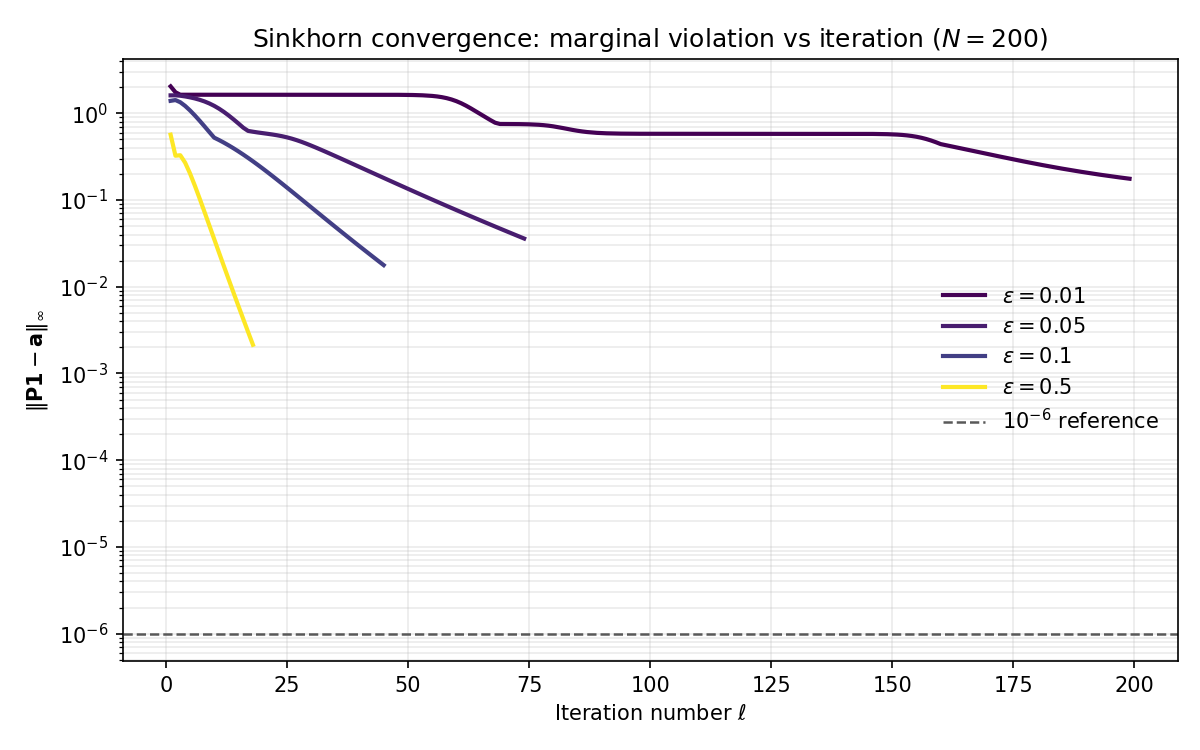
\includegraphics[width=0.85\linewidth]{sinkhorn_convergence.png}
    \caption{Sinkhorn iteration marginal violation $\|\mathbf{P}\mathbf{1} - \mathbf{a}\|_\infty$ vs iteration number $\ell$, for four regularisation strengths $\epsilon \in \{0.01, 0.05, 0.1, 0.5\}$ on the same $N = 200$ weighted cloud (seed $42$, log-normal weights). Smaller $\epsilon$ gives sharper transport plans but requires more iterations to reach the same tolerance.}
    \label{fig:sinkhorn_convergence}
\end{figure}

I ran $42$ implicit-backward gradient checks. Each case differentiates $\log p(z_{1:T}\mid\v\theta)$ with respect to one scalar parameter. The automatic-differentiation gradient is the derivative produced by differentiating through the whole differentiable filter pipeline, with Sinkhorn resampling using the implicit backward pass. The finite-difference reference uses central differences with base step $10^{-4}$ and five radii; the finite-difference median is the median of those five slopes. The relative error is
\begin{equation}
    \frac{\left|d_{\mathrm{AD}}-d_{\mathrm{FD}}\right|}
    {\max\!\left(\left|d_{\mathrm{FD}}\right|,10^{-12}\right)},
\end{equation}
The approximate-backward comparison is not in this table. The sweep I first made kept the particles fixed, so $d\mathbf{x}_k/d\v\theta=0$ and only Term 3 in Eq.~\ref{eq:ot-three-terms} fired. Approximate and implicit backward were then identical. That did not test the failure mode I care about, so I removed it from the report.

The columns in Table~\ref{tab:gradient_validation} mean the following. ``Cases'' is the number of $(T,\text{parameter value})$ configurations tested for that filter--model row. ``Parameter sweep'' names the single parameter that was varied and the values used at $T=20$; the same row also includes $T\in\{1,5,20\}$ at the nominal parameter. ``Median rel.\ err.'' and ``Max rel.\ err.'' are the median and maximum of the relative error above over the seven cases. ``Tolerance'' is the pass/fail threshold I set for that model. ``Pass'' means every one of the seven cases has relative error below that tolerance.

\begin{table}[H]
\centering
\footnotesize
\caption{Gradient validation summary. The columns are defined in the paragraph above the table; all rows use the implicit Sinkhorn backward.}
\label{tab:gradient_validation}
\begin{tabular}{lcccccc}
\toprule
Filter--model & Cases & Parameter sweep & Median rel.\ err. & Max rel.\ err. & Tolerance & Pass \\
\midrule
LG, LEDH+OT             & $7$ & $\sigma_{\mathrm{obs}} \in \{0.5, 1.0, 1.5, 2.0\}$ & $0.000510$ & $0.003200$ & $0.03$ & yes \\
LG, BPF+OT              & $7$ & $\sigma_{\mathrm{obs}} \in \{0.5, 1.0, 1.5, 2.0\}$ & $0.000120$ & $0.000410$ & $0.03$ & yes \\
RB, LEDH+OT             & $7$ & $\sigma_{\text{range}} \in \{0.05, 0.1, 0.2, 0.5\}$ & $0.000200$ & $0.001400$ & $0.08$ & yes \\
SV1D, LEDH+OT           & $7$ & $\alpha \in \{0.5, 0.7, 0.91, 0.95\}$ & $0.000650$ & $0.002000$ & $0.10$ & yes \\
SV2D, LEDH+OT ($N=200$) & $7$ & $\sigma_2 \in \{0.5, 1.0, 1.5, 2.0\}$ & $0.007500$ & $0.016000$ & $0.15$ & yes \\
SV2D, LEDH+OT ($N=500$) & $7$ & $\sigma_2 \in \{0.5, 1.0, 1.5, 2.0\}$ & $0.003500$ & $0.015000$ & $0.15$ & yes \\
\bottomrule
\end{tabular}
\end{table}

The numbers land as expected. LG is easy. Range-bearing and SV1D are still clean. SV2D is the hard row: the median error is about one order of magnitude larger than the easy models, but still below the $15\%$ tolerance I set for that model. Increasing SV2D from $N=200$ to $N=500$ lowers the median error but does not remove the worst case. That tells me the remaining error is not just particle count. It is the noisy nonlinear filter path plus the Sinkhorn backward.

Table~\ref{tab:gradient_validation} aggregates. Table~\ref{tab:gradient_validation_sv1d} shows the actual SV1D LEDH+OT rows so the median is not a black box.

\begin{table}[H]
\centering
\scriptsize
\caption{SV1D LEDH+OT gradient validation cases. The finite-difference slopes use radii $1,\ldots,5$ times the base step $10^{-4}$; the finite-difference median is the median of those five slopes.}
\label{tab:gradient_validation_sv1d}
\resizebox{\linewidth}{!}{%
\begin{tabular}{lccp{6.2cm}ccc}
\toprule
$T$ & $\alpha$ & FD slopes (5 radii) & FD median & automatic diff. & rel.\ err. \\
\midrule
 $1$  & $0.91$ & $-2.6973$, $-2.6973$, $-2.6973$, $-2.6974$, $-2.6974$ & $-2.6973$ & $-2.6973$ & $0.000013$ \\
 $5$  & $0.91$ & $0.1410$, $0.1410$, $0.1410$, $0.1409$, $0.1409$ & $0.1410$ & $0.1413$ & $0.002002$ \\
 $20$ & $0.91$ & $-1.8328$, $-1.8055$, $-1.8146$, $-1.8193$, $-1.8221$ & $-1.8193$ & $-1.8172$ & $0.001119$ \\
 $20$ & $0.50$ & $8.1123$, $8.1123$, $8.1123$, $8.1123$, $8.1123$ & $8.1123$ & $8.1132$ & $0.000108$ \\
 $20$ & $0.70$ & $10.9892$, $10.9892$, $10.9892$, $10.9892$, $10.9892$ & $10.9892$ & $10.9914$ & $0.000204$ \\
 $20$ & $0.91$ & $-1.8328$, $-1.8055$, $-1.8146$, $-1.8193$, $-1.8221$ & $-1.8193$ & $-1.8172$ & $0.001119$ \\
 $20$ & $0.95$ & $-20.2424$, $-20.2427$, $-20.2431$, $-20.2438$, $-20.2447$ & $-20.2431$ & $-20.2301$ & $0.000645$ \\
\bottomrule
\end{tabular}%
}
\end{table}

The finite-difference reference is stable where it should be stable. The $\alpha=0.5$, $\alpha=0.7$, and $\alpha=0.95$ rows barely move across the five radii. The repeated $T=20,\alpha=0.91$ row is noisier, but the five slopes still bracket the reported median and the automatic-differentiation value sits inside that spread. That is the check I care about. The relative-error column is only a compact summary of the same fact.


\subsection{Neural Acceleration}

\paragraph{The principle.}
A particle filter delivers $\{(x_i, w_i)\}$, a weighted realisation of a target distribution $q$. Resampling produces $\{(\tilde x_i, 1/N)\}$, an unweighted realisation of the \emph{same} $q$. Two different realisations of one continuous distribution; the job is to convert one into the other. Both have $N$ particles, so the natural framing is optimal transport: move mass from the weighted source to a uniform output that still approximates $q$.

\paragraph{What Sinkhorn does (recap).}
The OT-based resampler (\S\ref{sec:entropic-ot}) solves an OT problem with marginals $\mathbf{a} = \mathbf{w}$ and $\mathbf{b} = \tfrac{1}{N}\mathbf{1}$ on support $\{x_1, \ldots, x_N\}$ with L\textsuperscript{2} cost, then constructs output positions by barycentric projection $\hat x_i = N\sum_j P^*_{ji}\, x_j$ with uniform weight $1/N$. Reich's consistency theorem (\S\ref{sec:entropic-ot}) is what guarantees the output is asymptotically a realisation of $q$; the underlying $q$ enters the construction only through the source marginal $\mathbf{w}$. Cost is $\mathcal{O}(LN^2)$ per resampling step. A filter solves hundreds of nearby OT problems --- same structure, different cloud. That is the amortisation opportunity.

\paragraph{The neural map's design.}
Train a deterministic map $T : \mathbb{R}^d \to \mathbb{R}^d$ that takes an input particle position to an output position in one forward pass. For mass to be conserved point-by-point under such a map, the source has to carry uniform mass. That forces the framing:
\begin{itemize}
\item \textbf{Source:} $\mu_{\text{src}} = \tfrac{1}{N}\sum_i \delta_{x_i}$ --- same particles, weights flipped to uniform. Artificial.
\item \textbf{Target:} $\mu_{\text{tgt}} = \sum_i w_i \delta_{x_i}$ --- the weighted cloud the filter actually delivered.
\item \textbf{Map:} $T_\#\mu_{\text{src}} = \mu_{\text{tgt}}$.
\end{itemize}
Output is $\{(T(x_i), 1/N)\}$. The uniform-weight source is the price of replacing Sinkhorn's plan + barycentric projection with a single deterministic map. Sinkhorn's marginals carry mass conservation; the map version has to carry it pointwise via the Jacobian.

\paragraph{From discrete to continuous.}
A neural map cannot be trained against a sum of delta functions --- there is no gradient signal off the support. The standard fix is to smooth both measures with a Gaussian KDE of bandwidth $h$,
\begin{equation}
p_h(x) = \frac{1}{N}\sum_i K_h(x - x_i), \qquad
q_h(x) = \sum_i w_i K_h(x - x_i),
\end{equation}
which turns two discrete measures into two continuous densities on the same support. The map condition $T_\# p_h = q_h$ is the Monge--Amp\`ere equation
\begin{equation}
p_h(x) = q_h(T(x))\,\left|\det J_T(x)\right|.
\end{equation}
Smoothing is implementation; the principle is the previous paragraphs.

\paragraph{Loss and inference.}
Train $T(x;c)$ --- conditioned on a context $c$ from a permutation-invariant set encoder over the weighted cloud --- by minimising the squared log-residual of the Monge--Amp\`ere equation at points sampled from $p_h$:
\begin{equation}
L(c) = \mathbb{E}_{x \sim p_h}\!\left[\bigl(\log p_h(x) - \log q_h(T(x;c)) - \log\left|\det J_T(x;c)\right|\bigr)^2\right].
\end{equation}
At inference, encode the cloud once to get $c$, push every particle through the same map: $\tilde x_i = T(x_i; c)$, $\tilde w_i = 1/N$. One forward pass per resampling step instead of a Sinkhorn loop.

\paragraph{Status.}
Pipeline runs end-to-end. Current bug: the map fits its training cloud to near-zero residual but does not generalise. Next: train on a family of 2D Gaussian clouds (varying mean, covariance, weight skew); report the held-out residual.



%\begin{table}[htbp]
%\centering
%\caption{Resampling Method Comparison on Stochastic Volatility Model}
%\begin{tabular}{lcccccc}
%\toprule
%\textbf{Method} & \textbf{Param} & \textbf{RMSE} & \textbf{Log-Lik} & \textbf{Wall Time (s)} & \textbf{Time/Step (ms)} & \textbf{Resample Rate} \\
%\midrule
%\multicolumn{7}{l}{\textit{Baseline}} \\
%PF (Systematic) & ---    & 1.142 & $-547.56$ & 2.12  & 4.25  & 0.358 \\
%\midrule
%\multicolumn{7}{l}{\textit{Optimal Transport (OT) Resampling}} \\
%OT              & $\epsilon=0.1$ & 1.582 & $-702.84$ & 359.45 & 718.91 & 0.420 \\
%OT              & $\epsilon=0.3$ & 1.560 & $-839.05$ & 182.84 & 365.68 & 0.432 \\
%OT              & $\epsilon=0.5$ & 1.841 & $-703.65$ & 156.06 & 312.12 & 0.428 \\
%OT              & $\epsilon=1.0$ & 2.110 & $-723.65$ & 47.94  & 95.89  & 0.432 \\
%\midrule
%\multicolumn{7}{l}{\textit{Soft Resampling}} \\
%Soft            & $\alpha=0.5$   & 1.140 & $-545.37$ & 2.32  & 4.64  & 0.532 \\
%Soft            & $\alpha=0.7$   & 1.137 & $-544.05$ & 2.26  & 4.52  & 0.426 \\
%Soft            & $\alpha=0.9$   & 1.135 & $-545.60$ & 2.26  & 4.52  & 0.370 \\
%\bottomrule
%\end{tabular}
%\label{tab:stochastic_volatility_resampling}
%\end{table}
%PF (Systematic) works really well for Stochastic volatility model for the purpose of doing the filtering. We see that as we increase the $\epsilon$, the effect of smoothing out the particle distribution from OT resampling degrade the filtering result but it takes less time to run. Accuracy, namely less regularization requires more computation. Soft resampling is a modification of multinomial resampling, which is cheap to run, and less regularization is more accurate, consistent with OT resampling as well. 

\clearpage


%%%%%%%%%%%%%%%%%%%%%%%%%%%%%%%%%%%%%%%%%%%%%%%%%%%%%%%%%%
\newpage
\section{Parameter Estimation with Differentiable Particle Filters}
\label{sec:param-estimation}

\paragraph{Filtering accuracy is not gradient quality.} Section~\ref{sec:particle-methods-section} ranked filters by estimator accuracy: how close the filtered mean and covariance are to the true latent state, measured in RMSE and log-likelihood. This section ranks filters by \emph{gradient} quality: how well $\nabla_{\boldsymbol{\theta}} \log p_{\boldsymbol{\theta}}(z_{1:T})$ behaves under HMC. A filter can win the first ranking and lose the second, and vice versa --- a bootstrap filter with stop-gradient systematic resampling may track the state accurately yet hand HMC a discontinuous loss surface, while OT resampling often pays a $20$--$180\times$ compute tax depending on baseline and $\epsilon$, typically $60$--$100\times$ in HMC-relevant settings, that only shows up as useful gradient behaviour here. Keep the two criteria separate: §4 validates the filter as an estimator, §6 validates the filter as a differentiable subroutine in a parameter-inference pipeline.

\subsection{Markov Chain Monte Carlo}

\subsubsection{Metropolis-Hastings}
\label{sec:metropolis-hastings}

I want either the MAP point or the full posterior $p(\v \theta \mid z_{1:T})$ for the model parameters. The particle filter gives the marginal likelihood $p(z_{1:T} \mid \v \theta)$, and with a prior $p(\v \theta)$ the log-posterior is available up to a constant:
\begin{equation}
    \log p(\v \theta \mid z_{1:T}) = \log p(z_{1:T} \mid \v \theta) + \log p(\v \theta) + \text{const}.
    \label{eq:hmc-log-posterior}
\end{equation}
The question is how to explore this surface efficiently.

The simplest approach is a random walk in parameter space. Let $L(\v\theta) = -\log p(\v\theta \mid z_{1:T})$ denote the negative log-posterior. Propose a new parameter $\v \theta' = \v \theta + w$ where $w$ is a random vector, compute the change $\Delta L = L(\v \theta') - L(\v \theta)$, and always accept moves that improve the posterior ($\Delta L < 0$). Simply rejecting all uphill moves would trap the chain at the nearest local minimum. The Metropolis-Hastings algorithm \cite{Metropolis1953} accepts the proposed move with probability
\begin{equation}
    \alpha_{\mathrm{MH}} = \min\!\left(1,\; e^{-\Delta L}\right) = \min\!\left(1,\; \frac{p(\v \theta' \mid z_{1:T})}{p(\v \theta \mid z_{1:T})}\right).
    \label{eq:mh-acceptance}
\end{equation}
Even uphill moves get accepted with probability $e^{-\Delta L}$, allowing the chain to escape shallow local minima. This acceptance rule satisfies detailed balance, which guarantees the chain converges to the correct target distribution $p(\v \theta \mid z_{1:T})$. \\[6pt]
Random-walk MH has two failure modes.
\begin{enumerate}

\item The first is just finding the right region. Even with three parameters, the posterior does not fill the whole parameter space — it concentrates on a low-dimensional surface, a thin shell inside the 3D cube. This is the \textit{typical set}. Most of the volume is empty; the posterior mass lives on a much smaller manifold. In higher dimensions this only gets worse: the total volume grows exponentially while the typical set stays low-dimensional, so the fraction of space carrying any meaningful probability shrinks exponentially. A random walk has no way to seek out that manifold — it just stumbles around hoping to land on it.

\item The second problem shows up even after the chain has found the typical set. The step size $\varepsilon$ in the proposal $\v\theta' = \v\theta + \varepsilon\,\xi$, $\xi \sim \mathcal{N}(0, I)$, is the radius of the proposal ball. To see why $\varepsilon$ must shrink with dimension, consider a simple illustrative case: $d$ independent standard Gaussian coordinates, $\log p(\v\theta) = -\tfrac{1}{2}\|\v\theta\|^2 + \text{const}$. The change in log-posterior for coordinate $i$ after a step $\varepsilon\xi_i$ is exactly
\begin{equation}
    \Delta\log p_i = -\varepsilon\theta_i\xi_i - \frac{\varepsilon^2\xi_i^2}{2}.
\end{equation}
The first term has mean zero and standard deviation $\varepsilon|\theta_i| \sim \varepsilon$ for a typical $\theta_i \sim \mathcal{N}(0,1)$. The second term has mean $-\varepsilon^2/2$ since $\mathbb{E}[\xi_i^2] = 1$. Summing over all $d$ coordinates, the total change in log-posterior has
\begin{equation}
    \mathbb{E}[\Delta\log p] = -\frac{\varepsilon^2 d}{2}, \qquad \mathrm{std}[\Delta\log p] \sim \varepsilon\sqrt{d}.
\end{equation}
For the acceptance rate not to collapse, the mean must not be overwhelmingly negative: $\varepsilon^2 d = \mathcal{O}(1)$, which gives $\varepsilon = \mathcal{O}(d^{-1/2})$. The step size shrinks not because any single direction is narrow, but because perturbations accumulate across all $d$ dimensions at once. With $\varepsilon \sim d^{-1/2}$, the chain takes $\mathcal{O}(d)$ steps to move a meaningful distance — exploration becomes quadratically more expensive as dimension grows.

\end{enumerate}
\subsubsection{Hamiltonian Monte Carlo}

When the pipeline is fully differentiable, I can do much better. HMC is a method for sampling from the \emph{target it is given}. The Metropolis correction compensates for numerical integrator error under that target; it does not cleanse a biased or noisy particle-filter marginal likelihood and turn it into an exact posterior. Whatever bias is present in the log-likelihood surface from stop-gradient systematic resampling or the single-step Sinkhorn-backward approximation survives into HMC's stationary distribution. Hamiltonian Monte Carlo (HMC) \cite{Duane1987,Neal-2012-MCMC-Hamiltonian-Dynamics-ARXIV-1206-1901v1} treats parameter estimation as a physical dynamics problem. I introduce an auxiliary momentum variable $\v p$ of the same dimension as $\v \theta$ and define the Hamiltonian:
\begin{equation}
    H(\v p, \v \theta) = \underbrace{\frac{1}{2}\v p^\top M^{-1} \v p}_{K(\v p) \text{ (kinetic)}} + \underbrace{U(\v \theta)}_{\text{(potential)}}
\end{equation}
where $U(\v \theta) = -\log p(\v \theta \mid z_{1:T})$ is the negative log-posterior and $M$ is the mass matrix. Think of a ball rolling in a potential landscape: the ball picks up speed going downhill and slows going uphill, efficiently exploring the landscape while conserving total energy. Hamilton's equations describe the trajectory:
\begin{equation}
    \frac{d\v \theta}{dt} = M^{-1}\v p, \qquad \frac{d\v p}{dt} = -\nabla_{\v \theta} U(\v \theta).
\end{equation}
These trajectories conserve $H$ exactly, so the ball naturally curves around the posterior contours rather than wandering randomly.

\paragraph{Leapfrog integration.}
In practice I integrate Hamilton's equations numerically with the \textit{leapfrog} (Störmer-Verlet) integrator, which alternates half-step momentum updates and full-step position updates. Concretely, with step size $\varepsilon$ and $L$ steps:
\begin{align}
    \v p_{t+\frac{1}{2}} &\leftarrow \v p_t - \tfrac{\varepsilon}{2}\nabla_{\v \theta} U(\v \theta_t) \notag \\
    \v \theta_{t+1} &\leftarrow \v \theta_t + \varepsilon M^{-1} \v p_{t+\frac{1}{2}} \notag \\
    \v p_{t+1} &\leftarrow \v p_{t+\frac{1}{2}} - \tfrac{\varepsilon}{2}\nabla_{\v \theta} U(\v \theta_{t+1}) \notag
\end{align}
The leapfrog scheme is symplectic, meaning it approximately conserves $H$ even over many steps. Each HMC iteration samples a fresh momentum $\v p \sim \mathcal{N}(0, M)$, runs $L$ leapfrog steps to produce a proposal $(\v \theta^*, \v p^*)$, then accepts with the Metropolis criterion:
\begin{equation}
    \alpha_{\mathrm{HMC}} = \min\!\left(1,\; e^{-(H(\v p^*, \v \theta^*) - H(\v p, \v \theta))}\right).
    \label{eq:hmc-acceptance}
\end{equation}
Because the leapfrog nearly conserves $H$, the energy difference $\Delta H \approx 0$ and the acceptance probability is close to 1, even for proposals far from the current point. This is the key advantage over random-walk MH: the momentum carries the state along energy contours, allowing large, directed moves. Two properties are therefore non-negotiable: $\nabla_{\boldsymbol{\theta}} U$ must be bounded (a single spike derails the trajectory and wastes the proposal) and $U(\boldsymbol{\theta})$ must be continuous (discontinuities cause $\Delta H$ to jump and the Metropolis correction to reject). This is exactly the demand that \S\ref{sec:ot-derivative-chain} places on the resampling derivative chain; HMC's acceptance rate is the empirical test of whether the chain delivers.

\paragraph{Step size and tuning.}
The leapfrog integrator approximates the continuous Hamiltonian trajectory with finite steps of size $\varepsilon$. If $\varepsilon$ is too large, the numerical integration accumulates error, $H$ is no longer conserved, and $\Delta H$ becomes large — the Metropolis correction then rejects most proposals and the chain stalls. If $\varepsilon$ is too small, each accepted step moves only a tiny distance and the chain explores slowly. The acceptance rate is therefore a direct readout of whether $\varepsilon$ is well-calibrated: too low means overshooting; too high means nearly standing still.

I initialize $\varepsilon = 0.01$ and let it self-adapt during the first $80\%$ of burn-in iterations via dual averaging \cite{hoffman2014nuts}, which adjusts $\varepsilon$ to hit a target acceptance rate of $65\%$. Let $\delta$ be the target acceptance rate and $\alpha_m$ the actual acceptance rate at step $m$. The update equations are:
\begin{align}
\bar{H}_m &= \left(1 - \frac{1}{m + t_0}\right)\bar{H}_{m-1} + \frac{1}{m + t_0}(\delta - \alpha_m), \\
\log \varepsilon_m &= \mu - \frac{\sqrt{m}}{\gamma}\,\bar{H}_m, \\
\log \bar{\varepsilon}_m &= m^{-\kappa}\log \varepsilon_m + (1 - m^{-\kappa})\log \bar{\varepsilon}_{m-1}.
\end{align}
Here $\mu = \log(10\varepsilon_0)$ is the reference target, $\gamma = 0.05$ is a shrinkage factor, $t_0 = 10$ stabilises early iterations, and $\kappa = 0.75$ controls the long-run averaging weight. The running average $\bar{\varepsilon}_m$ is used as the fixed step size after adaptation ends. I also monitor the gradient norm $\|\nabla U\|$ at each leapfrog step: a gradient that spikes or produces a non-finite value is not a tuning problem --- it signals numerical instability somewhere in the model or filter pipeline.

\paragraph{Mass matrix.}
Start from a well-chosen coordinate system. In physics, for a system that is not over-constrained, the right parameterization decouples the dynamics into independent trajectories. Think of describing a circle: polar coordinates $(r,\phi)$ decouple the radial and angular motion immediately, while Cartesian $(x,y)$ keep them entangled. The same principle applies here — if the posterior directions are strongly coupled or have very different scales, the ball's trajectory mixes up slow and fast modes and explores inefficiently.

The mass matrix $M$ is how I implement this rescaling within HMC without changing the parameterization itself. At each iteration I sample a fresh momentum $\v p \sim \mathcal{N}(0, M)$, so $M_{ii}$ controls how much kinetic energy is injected in direction $i$ before the ball starts rolling. Think of each parameter direction as an independent harmonic oscillator — some with a steep potential (narrow posterior, high curvature) and some with a flat potential (wide posterior, low curvature). A steep direction needs more initial kinetic energy to escape the narrow well and explore; a flat one needs less. Setting $M_{ii}$ proportional to the posterior variance in direction $i$ balances the energy across modes so that all directions are explored at a similar rate.

I use a fixed diagonal mass matrix specified as a vector of per-parameter values. The default is the identity ($M = I$), and the values are set manually based on the expected scale of each parameter. A full production setup would run a short pilot chain, estimate the empirical per-parameter variance, and set the diagonal entries from that --- but for the benchmarks here, the parameters are well-understood enough that the scales can be set directly.

\subsubsection{MCMC Diagnostics}

After every HMC run I report four diagnostics.

\paragraph{Acceptance rate.}
Equation~\ref{eq:hmc-acceptance} gives the HMC acceptance rule. If the leapfrog integrator were exact, $\Delta H = 0$ and every proposal would be accepted. Numerical discretisation error causes $\Delta H \neq 0$, so some proposals are rejected. The acceptance rate is therefore a direct diagnostic for step size calibration: too low means the step size is too large and the trajectory overshoots; too high (near 100\%) means the step size is too small and the chain barely moves. I target $65\%$ acceptance, which is the theoretically optimal rate for high-dimensional Gaussian targets \cite{beskos2013optimal}.

\paragraph{Effective sample size (ESS).}
Because consecutive MCMC samples are correlated, $N$ correlated samples carry less information than $N$ independent ones. The effective sample size quantifies this:
\begin{equation}
\mathrm{ESS} = \frac{N}{1 + 2\sum_{k=1}^{\infty} \rho_k},
\label{eq:ess-def}
\end{equation}
where $\rho_k = \mathrm{Corr}(\theta_t, \theta_{t+k})$ is the lag-$k$ autocorrelation of the chain. For an AR(1) chain $\theta_t = \phi\,\theta_{t-1} + \varepsilon_t$ with $|\phi| < 1$, $\rho_k = \phi^k$ and $\mathrm{ESS} = N(1-\phi)/(1+\phi)$. With $N = 200$ samples, $\phi = 0.9$ gives ESS $\approx 11$ --- the chain is exploring very slowly. $\phi = 0$ gives ESS $= 200$ --- fully independent.

\subparagraph{Computing $\rho_k$ from the chain.}
For a finite chain $\{\theta_1, \ldots, \theta_N\}$ with sample mean $\bar\theta = N^{-1}\sum_t \theta_t$, the (biased) sample autocovariance and autocorrelation at lag $k$ are
\begin{equation}
c_k = \frac{1}{N}\sum_{t=1}^{N-k} (\theta_t - \bar\theta)(\theta_{t+k} - \bar\theta), \qquad
\hat\rho_k = \frac{c_k}{c_0}, \qquad k = 0, 1, \ldots, N-1.
\label{eq:autocorr-def}
\end{equation}
The biased estimator $c_k$ has $1/N$ rather than $1/(N-k)$ in the denominator; this regularises the high-lag tail and is the convention used in MCMC ESS estimation. Computing all $N$ lags directly costs $\mathcal{O}(N^2)$, so I use the standard FFT recipe: zero-pad the centered chain $y_t = \theta_t - \bar\theta$ to length $2N$, take the FFT $Y = \mathrm{FFT}(y)$, and recover the autocovariances as
\begin{equation}
(c_0, c_1, \ldots, c_{N-1}) = \frac{1}{N}\,\mathrm{Re}\bigl[\mathrm{IFFT}\bigl(|Y|^2\bigr)\bigr]_{0:N},
\label{eq:autocorr-fft}
\end{equation}
which costs $\mathcal{O}(N \log N)$. This works because the inverse FFT of the power spectrum $|Y|^2$ is the circular autocorrelation; zero-padding to $2N$ before the FFT removes the wrap-around, leaving the linear autocorrelation in the first $N$ entries.

\subparagraph{Truncating the infinite sum.}
Equation~\ref{eq:ess-def} sums to $k = \infty$, but $\hat\rho_k$ becomes pure noise once the true autocorrelation has decayed. I use Geyer's initial monotone sequence rule: form the lag pairs $\hat\Gamma_m = \hat\rho_{2m} + \hat\rho_{2m+1}$, take the running minimum, and truncate at the first $m$ where $\hat\Gamma_m \le 0$. The integrated autocorrelation time is then
\[
\hat\tau = 1 + 2\sum_{m=0}^{m^\star-1} \hat\Gamma_m, \qquad \mathrm{ESS} = N / \hat\tau.
\]
For multi-chain ESS I average $\hat\rho_k$ across chains before pairing; this is the recipe used in Stan's diagnostics package and in the ArviZ implementation I cross-checked against. With fewer than a few hundred samples the estimator is noisy and ESS can saturate at $N$ even when mixing is imperfect.

\paragraph{$\hat{R}$: Potential Scale Reduction Factor.}
$\hat{R}$ (Gelman \& Rubin, 1992) detects non-convergence by comparing \emph{within-chain} to \emph{between-chain} variance. Since I run a single chain, I split the $N$ post-burn-in samples into two halves of length $n = N/2$ and treat them as two independent chains. Let $\bar\theta_j$ and $s_j^2$ be the mean and variance of chain $j$ ($j = 1, 2$). Define:
\begin{align}
W &= \tfrac{1}{2}(s_1^2 + s_2^2) && \text{(within-chain variance)}, \\
B &= n\,(\bar\theta_1 - \bar\theta_2)^2 / 2 && \text{(between-chain variance)}, \\
\hat{V} &= \tfrac{n-1}{n}\,W + \tfrac{1}{n}\,B && \text{(pooled variance estimate)}.
\end{align}
Then $\hat{R} = \sqrt{\hat{V}/W}$. If the chain has converged, both halves look like draws from the same distribution, so $B \approx 0$ and $\hat{R} \approx 1$. This is a \emph{split} $\hat{R}$ from a single chain, which is a rough one-chain diagnostic --- it detects gross non-stationarity within a run but is not a substitute for a true multi-chain $\hat{R}$, which would compare independent chains initialised from over-dispersed starting points. The standard threshold is $\hat{R} > 1.1$ to flag non-convergence. Values slightly below 1 are an artifact of finite-sample estimation and are harmless. With only $n = 100$ samples per half, both $W$ and $B$ are estimated noisily, so at least $N \geq 400$ total samples are recommended before trusting $\hat{R}$.

\paragraph{Multi-chain split-$\hat R$.}
For the four-chain runs reported in \S\ref{sec:hmc-multichain}, I compute the modern split $\hat R$ from Vehtari et al.\ (2021). Given $M = 4$ independent chains of $N$ post-burn-in samples each, I first split each chain in half to give $M' = 2M = 8$ ``half-chains'' of length $n = N/2$. Let $\bar\theta_j$ and $s_j^2$ denote the mean and variance of half-chain $j$, $j = 1, \ldots, M'$. The between-chain and within-chain variances become
\begin{align}
W &= \frac{1}{M'}\sum_{j=1}^{M'} s_j^2&& \text{(within-chain variance)}, \\
B &= \frac{n}{M' - 1}\sum_{j=1}^{M'} \bigl(\bar\theta_j - \bar{\bar\theta}\bigr)^2 && \text{(between-chain variance)}, \\
\hat V &= \frac{n-1}{n} W + \frac{1}{n} B, \qquad \hat R = \sqrt{\hat V / W},
\label{eq:rhat-multichain}
\end{align}
where $\bar{\bar\theta} = M'^{-1}\sum_j \bar\theta_j$ is the grand mean. The split halves contribute the within-run non-stationarity check; the four independent chains starting from over-dispersed inits contribute the between-run mixing check. With $M = 4$ and $N = 400$, the $\hat R$ estimator is well-conditioned, and the modern threshold $\hat R \le 1.01$ replaces the older $\hat R \le 1.1$.

\subparagraph{Rank-normalized $\hat R$ (Stan default).}
Equation~\ref{eq:rhat-multichain} compares chain means and variances. That makes it sensitive to mean and second-moment differences across chains but blind to higher-moment mismatches and very vulnerable to heavy tails: a single outlier sample can dominate $s_j^2$ and pull $\hat R$ either above or below $1$ in misleading ways. The Vehtari et al.\ (2021) fix is to apply the same machinery to a rank-normalized chain instead. Pool all $MN$ samples, replace each by its (continuous) rank
\[
r_t^{(m)} = \mathrm{rank}\bigl(\theta_t^{(m)}\bigr), \qquad z_t^{(m)} = \Phi^{-1}\!\left(\frac{r_t^{(m)} - 3/8}{MN + 1/4}\right),
\]
where $\Phi^{-1}$ is the standard normal quantile, then run Eq.~\ref{eq:rhat-multichain} on $z$. The rank trick whitens the problem before ANOVA: ranks are uniform under the null regardless of the true posterior shape, so the moment-based recipe becomes sensitive to \emph{any} difference in distribution across chains, not just mean/variance, while the $\Phi^{-1}$ map keeps the $W$, $B$ statistics on a familiar scale. I report this as \emph{bulk}-$\hat R$. To catch scale and tail mismatches that bulk-$\hat R$ can miss, I also fold each sample around the pooled median, $\tilde\theta_t^{(m)} = |\theta_t^{(m)} - \mathrm{median}(\theta)|$, rank-normalize the folded values, and compute $\hat R$ again --- this is \emph{tail}-$\hat R$. Stan reports $\max(\mathrm{bulk}\text{-}\hat R, \mathrm{tail}\text{-}\hat R)$ and so do I; all converged runs in \S\ref{sec:hmc-multichain} have $\max\hat R \le 1.008$ (Kalman and SV1D are the worst at $1.008$ and $1.005$; LEDH+OT, BPF+OT, EKF, UKF, and the range-bearing axes all sit below $1.007$), comfortably under the $1.01$ threshold. I report $\hat R$ alongside two ESS variants: \emph{bulk ESS}, computed as the ESS on the rank-normalized pooled samples (same $z_t^{(m)}$ as bulk-$\hat R$), and \emph{tail ESS}, the minimum of the ESS on the indicator that samples exceed the $5\%$ and $95\%$ quantiles, which catches mixing problems that show up only in the posterior tails.

\subsection{Parameter Prior Selection}
\label{sec:param-prior-selection}

\paragraph{What the prior is doing here.}
There are two different priors in this section, and I keep them separate. The filter has an initial-state prior over $x_0$; that is the Lyapunov or physical prior described in \S\ref{par:init-conditions}. HMC has a parameter prior $p(\v\theta)$ over the unknown constants that I am estimating. This subsection is about the second object. Recall the log-posterior decomposition in Eq.~\ref{eq:hmc-log-posterior}; the choices here specify the $p(\v\theta)$ term in that equation.
I chose these priors because the likelihood comes from a particle filter, not from an exact analytic marginal likelihood. A very diffuse prior lets HMC spend time in parameter regions where the filter degenerates, the ESS collapses, or the gradient is dominated by numerical artifacts. A prior that is too tight can hide a real model mismatch. The compromise I used is weakly informative and physical-scale based: center the prior near the known synthetic truth for benchmark runs, but keep enough width that the data can still move the posterior.

\paragraph{Families I used.}
For positive scale parameters I use $\mathrm{LogNormal}(\mu,\sigma)$. This is not just a generic Bayesian default. Noise scales are multiplicative objects: being wrong by a factor of two is a natural error, being wrong by an additive $0.2$ is not. A $\mathrm{LogNormal}(\mu,\sigma)$ also fits HMC because the parameter is positive in the model but unconstrained in the sampler. For $\mathrm{LogNormal}(\mu,s)$, the median is $\exp(\mu)$ and the mode is $\exp(\mu-s^2)$. This matters. MAP is pulled by the mode; HMC spends mass around the median and mean. The working guide therefore recommends $s=0.5$ as the default weakly informative scale, and warns that $s=1.0$ gives a very wide order-of-magnitude prior. For bounded persistence parameters I prefer a $\mathrm{Beta}(\alpha,\beta)$ prior when I have real knowledge that the process is persistent. A $\mathrm{Uniform}(0,1)$ prior is sometimes present in the current configurations, but I treat it as a sensitivity or legacy choice because it gives HMC no help near the boundaries. Table~\ref{tab:param-priors} lists the priors actually used in the HMC configurations.

\begin{table}[H]
\centering
\scriptsize
\caption{Parameter priors used by the HMC configurations.}
\label{tab:param-priors}
\begin{tabular}{p{2.4cm}p{2.4cm}p{2.5cm}p{2.1cm}p{2.0cm}p{3.4cm}}
\toprule
Model & Parameter & Prior family & Parameters & Support & Why this prior \\
\midrule
Linear Gaussian full & process noise std & $\mathrm{LogNormal}(\mu,\sigma)$ & loc $=0.0$, scale $=1.0$ & positive & Median $1.0$ matches the unit noise scale, but the guide flags scale $1.0$ as wider than needed. \\
Linear Gaussian full & observation noise std & $\mathrm{LogNormal}(\mu,\sigma)$ & loc $=0.0$, scale $=1.0$ & positive & Same scale logic; useful for HMC but its MAP mode is only $\exp(-1)\approx0.37$. \\
1D SV & $\alpha$ & $\mathrm{LogNormal}(\mu,\sigma)$ & loc $=-0.094$, scale $=0.5$ & positive & Median near $0.91$ matches the synthetic persistence; this configuration does not enforce $\alpha<1$. \\
1D SV & $\sigma$ & $\mathrm{LogNormal}(\mu,\sigma)$ & loc $=0.0$, scale $=0.5$ & positive & Median $1.0$ matches the latent innovation scale with factor-of-$2$ uncertainty. \\
1D SV & $\beta$ & $\mathrm{LogNormal}(\mu,\sigma)$ & loc $=-0.693$, scale $=0.5$ & positive & Median $0.5$ matches the observation scale used to generate the data. \\
SV2D all-parameter HMC & $a_1$ & $\mathrm{Uniform}(a,b)$ & low $=0.0$, high $=1.0$ & $(0.001,0.999)$ in the transform & Legacy weak prior for a stable persistence coefficient; the guide would prefer an informative $\mathrm{Beta}(\alpha,\beta)$ when persistence is known. \\
SV2D all-parameter HMC & $a_2$ & $\mathrm{Uniform}(a,b)$ & low $=0.0$, high $=1.0$ & $(0.001,0.999)$ in the transform & Same persistence rationale; this prior deliberately does not rule out low-persistence regimes. \\
SV2D all-parameter HMC & $\sigma_1$ & $\mathrm{LogNormal}(\mu,\sigma)$ & loc $=-0.7$, scale $=0.5$ & positive & Median $\approx0.50$ matches the first process-noise scale. \\
SV2D all-parameter HMC & $\sigma_2$ & $\mathrm{LogNormal}(\mu,\sigma)$ & loc $=0.0$, scale $=0.5$ & positive & Median $1.0$ matches the second process-noise scale; the guide calls this well aligned. \\
Range-bearing & $\sigma_{\mathrm{range}}$ & $\mathrm{LogNormal}(\mu,\sigma)$ & loc $=-2.3$, scale $=0.5$ & positive & Median $\approx0.1$ because range noise is known to be order $10^{-1}$. \\
Range-bearing & $\sigma_{\mathrm{bearing}}$ & $\mathrm{LogNormal}(\mu,\sigma)$ & loc $=-2.3$, scale $=0.5$ & positive & Same physical noise scale for bearing in the benchmark configuration. \\
\bottomrule
\end{tabular}
\end{table}

\paragraph{Bijectors and the Jacobian term.}
The model parameters live on constrained spaces: noise standard deviations must be positive, persistence parameters must stay inside an interval, and HMC itself wants to move in an unconstrained Euclidean space. I handle this with smooth bijections: a positive transform maps unconstrained coordinates to scale parameters, and a scaled logistic transform maps to bounded intervals. The log prior is evaluated in the constrained parameter value and then the forward log-Jacobian of the bijector is added. This is the change-of-variables correction. Without it, HMC would sample the wrong density in the unconstrained coordinate, even if the constrained prior looked correct on paper.

\paragraph{Effect on HMC.}
The prior changes the geometry that HMC sees. A tighter, correctly centered prior reduces wasted exploration in regions where the particle filter is numerically bad, so ESS and acceptance can improve. The cost is bias if I centered the prior on the wrong physical scale. A weakly informative prior is the safer default when I know the order of magnitude but do not want to overfit the benchmark truth. This is why I do not use textbook ``noninformative'' inverse-gamma or very wide log-normal priors here. Those are designed for cleaner likelihoods than the one produced by a differentiable particle filter.

\paragraph{Worked example: range-bearing noise.}
For range-bearing, the observation noise scale is physically around $0.1$ in both coordinates in the benchmark. I therefore set the prior median near $0.1$, not near $1.0$. The numeric prior location is $-2.3$, because $\log(0.1)=-2.3026$. With scale $0.5$, the prior is wide enough to cover roughly a factor of $2$--$3$ around that value, but it does not send HMC into absurd noise scales where the likelihood surface is dominated by particle collapse. The constrained parameter is positive, so the sampler moves in an unconstrained coordinate $u$, the positive transform produces $\sigma=s(u)$, and the HMC potential receives
\begin{equation}
    U(u) = -\log p(z_{1:T}\mid \sigma) - \log p(\sigma) - \log\left|\frac{d\sigma}{du}\right|.
\end{equation}
That last term is easy to forget. It is why the prior is not just the $\mathrm{LogNormal}(\mu,\sigma)$ density in constrained space; it is that density plus the transform correction needed to sample the same target in unconstrained HMC coordinates.

%\paragraph{Config discrepancies.}
%The working guide and the run configurations are not perfectly aligned. The guide recommends $\mathrm{LogNormal}(0.25, 0.5)$ for the linear-Gaussian noise scales if MAP mode alignment is the priority, but the reported HMC runs still use $\mathrm{LogNormal}(0.0, 1.0)$. The guide also prefers $\mathrm{Beta}(\alpha,\beta)$-style priors for bounded persistence parameters; the SV2D all-parameter HMC configuration uses $\mathrm{Uniform}(0,1)$ for $a_1$ and $a_2$, while the 1D SV configuration uses a $\mathrm{Beta}(\alpha,\beta)$ prior for $\alpha$. Finally, the SV2D $\sigma_2$-only HMC configuration sets $\sigma_2\sim\mathrm{LogNormal}(0.25,0.5)$ to put the mode at $1.0$, while the all-parameter configuration uses loc $=0.0$ to put the median at $1.0$.
% I record these differences rather than smoothing them over, because they affect whether MAP or HMC is the intended diagnostic.

%\paragraph{What I used vs.\ what the guide recommends (known limitations).}
%The table above records the priors that actually entered the HMC runs. The working guide goes one step further and says which of those choices I should update. I did not make those config changes before producing the reported runs, so this is a known limitation of the parameter-inference section, not a correction to the experiments.

%\begin{table}[H]
%\centering
%\scriptsize
%\caption{Known prior-selection discrepancies between the HMC configs and the working guide.}
%\label{tab:param-prior-discrepancies}
%\begin{tabular}{p{3.0cm}p{3.5cm}p{3.5cm}p{3.0cm}}
%\toprule
%Model / parameter & Used & Recommended & Status \\
%\midrule
%Linear Gaussian observation noise & $\mathrm{LogNormal}(0.0,1.0)$ & $\mathrm{LogNormal}(0.25,0.5)$, so the prior peak better matches MAP estimates and the prior is tighter & Not updated; report runs use $\mathrm{LogNormal}(0.0,1.0)$ \\
%SV2D persistence in all-parameter HMC & $\mathrm{Uniform}(0,1)$ for $a_1$ and $a_2$ & $\mathrm{Beta}(10,2)$ mapped through a scaled logistic transform onto $(0.001,0.999)$ & Not updated; this likely contributes to weak localisation in the SV2D HMC failure \\
%SV2D $\sigma_2$ across sibling configurations & One $\sigma_2$-only configuration uses loc $=0.25$; the smoke and all-parameter configurations use loc $=0.0$ & Use loc $=0.25$ consistently when the goal is mode $=1.0$ for scale $=0.5$ & Partial; standalone configuration is mode-corrected, siblings and guide table are stale \\
%\bottomrule
%\%end{tabular}
%\end{table}

%I did not apply these updates to the runs in this report due to time constraints. The $\sigma_2$-only configuration has been partially mode-corrected but the sibling configurations and the guide table itself have not been synced. A future iteration should (i) switch linear-Gaussian observation-noise priors to $\mathrm{LogNormal}(0.25, 0.5)$, (ii) replace the SV2D $\mathrm{Uniform}(0,1)$ persistence prior with $\mathrm{Beta}(10, 2)$ via a scaled logistic transform, (iii) propagate the $\sigma_2$ mode-accurate loc $=0.25$ to all SV2D HMC configurations, and (iv) re-run the linear-Gaussian and SV2D benchmarks under the updated priors. The SV2D failure mode in \S\ref{sec:sv2d} may partially lift under the informative $\mathrm{Beta}(\alpha,\beta)$ prior, but I cannot claim so without rerunning.

\subsection{MAP as a Pipeline Smoke Test}
\label{sec:map-smoke-test}

Run MAP before HMC. MAP finds the mode of the posterior by gradient descent on $U(\v \theta) = -\log p(\v \theta \mid z_{1:T})$,
\begin{equation}
    \v \theta \leftarrow \v \theta - \eta \nabla_{\v \theta} U(\v \theta),
\end{equation}
using Adam or SGD. I run MAP in two modes. The \emph{fresh-seed} mode draws a new particle-filter seed at every gradient step, so resampling discontinuities average out over the trajectory; this is the default diagnostic and is useful for checking that the pipeline converges at all. The \emph{fixed-seed} mode holds the particle seed constant across optimizer steps, which exposes the same discontinuities HMC will see during a single leapfrog trajectory --- if fixed-seed MAP converges cleanly, fixed-seed HMC is much more likely to follow suit. MAP is more tolerant than HMC of imperfect resampling gradients in two ways. First, it does not require a globally smooth loss surface: fresh-seed stochastic gradients average out occasional discontinuities, and even fixed-seed MAP only needs the gradient to point roughly downhill on average. Second, it does not require unbiased gradients carrying full information. MAP will therefore often succeed with simple stop-gradient systematic resampling where HMC cannot --- but this is tolerance, not immunity: on sharply discontinuous surfaces (e.g., the SV2D pipeline that drives the open failure case noted in the Limitations subsection) even MAP can fail, so a clean MAP run is a necessary but not sufficient condition for HMC to work.

The reason this matters is diagnostic: if MAP fails—loss diverges, gradients blow up, or the parameters drift away from the truth—there is a numerical problem somewhere in the model or filter pipeline. MAP is therefore the first benchmark before HMC. I treat MAP convergence on a known model (e.g., 1-D linear Gaussian) as the minimum bar that any new filter configuration must clear. Only once MAP works cleanly do I move to HMC, which has the additional requirements of a deterministic loss surface (fixed particle seed) and smooth gradients.
The prior in the MAP objective is not a resampling choice; I use the same parameter prior for MAP and HMC and explain the selection in \S\ref{sec:param-prior-selection}.

\paragraph{MAP convergence across four benchmarks.}
I ran MAP on four models as the pipeline smoke test: 1D linear Gaussian (where both BPF+OT and LEDH+OT were exercised so that I could verify the differentiable filter does not introduce a filter-family bias), range-bearing with LEDH+OT (two parameters, $\sigma_{\text{range}}$ and $\sigma_{\text{bearing}}$, estimated jointly), 1D stochastic volatility with LEDH+OT (estimating the persistence $\alpha$), and 2D stochastic volatility with LEDH+OT (estimating $\sigma_2$). Every run uses a single cosine warm-down learning-rate schedule shared across benchmarks; Figure~\ref{fig:map_learning_rate} confirms the schedules overlap exactly on the four runs, so the convergence differences that follow are not an artifact of tuning. Figures~\ref{fig:map_lg}, \ref{fig:map_rb}, \ref{fig:map_sv1d}, and~\ref{fig:map_sv2d} show the four convergence traces.

\begin{figure}[H]
    \centering
    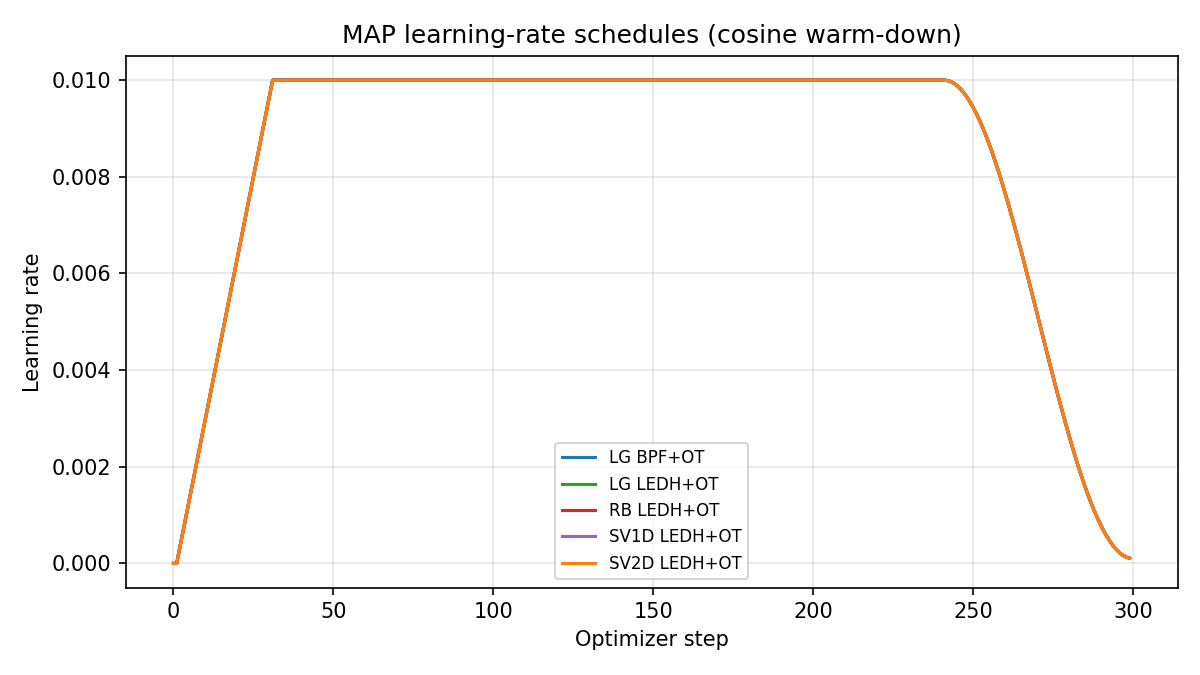
\includegraphics[width=0.8\linewidth]{map_learning_rate.png}
    \caption{Learning-rate schedules for the four MAP runs. All four use the same cosine warm-down schedule; the curves overlap exactly, so any convergence-speed differences in the figures below come from the loss surface, not from tuning.}
    \label{fig:map_learning_rate}
\end{figure}

Each of the four MAP convergence figures is a three-panel composite: top panel shows the negative log-likelihood $-\log p(z_{1:T} \mid \boldsymbol{\theta})$ at each optimizer step (the MAP objective up to the prior term), middle panel shows the gradient norm $\lVert\nabla_{\boldsymbol{\theta}} U\rVert$, and bottom panel shows the parameter trajectory with the true data-generation value as a horizontal dashed line.

\begin{figure}[H]
    \centering
    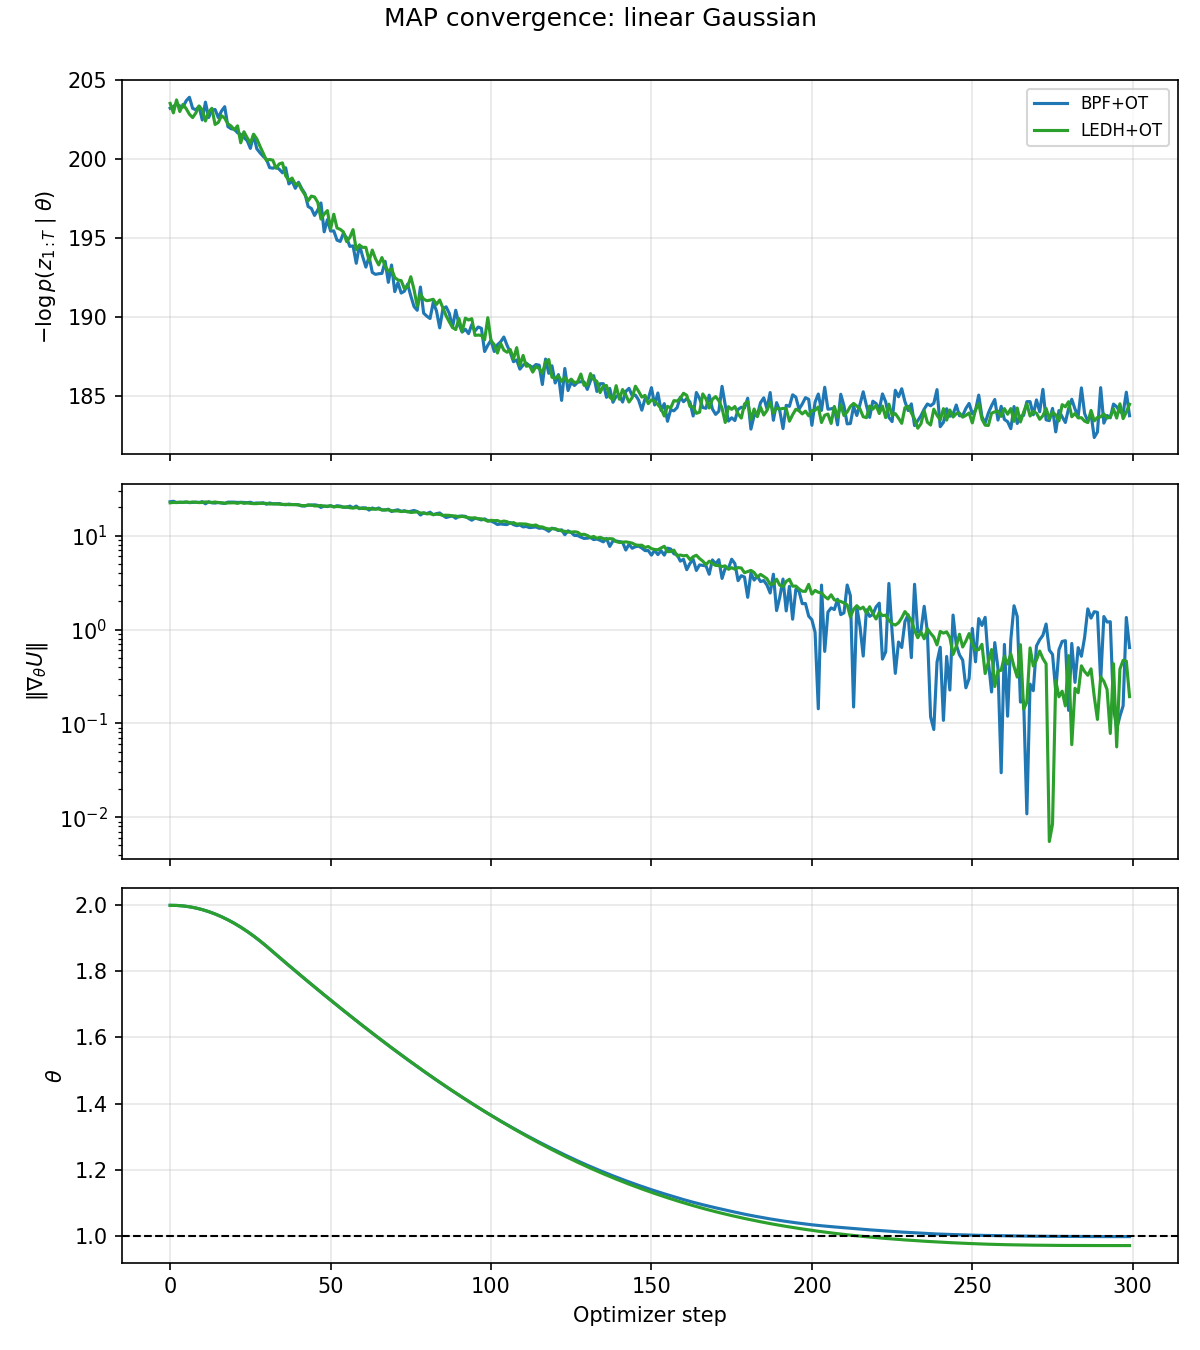
\includegraphics[width=0.82\linewidth]{map_lg.png}
    \caption{MAP convergence on the 1D linear Gaussian benchmark, with BPF+OT (blue) and LEDH+OT (green) running the same optimizer schedule against the same data. Both filters converge to the same neighbourhood of the true $\sigma_{\text{obs}} = 1.0$; the fact that LEDH+OT --- which passes the full three-term derivative chain --- matches BPF+OT (where only the weight gradient is active) is the cleanest check that the flow-filter gradient path is not introducing a systematic bias on linear Gaussian targets.}
    \label{fig:map_lg}
\end{figure}

\begin{figure}[H]
    \centering
    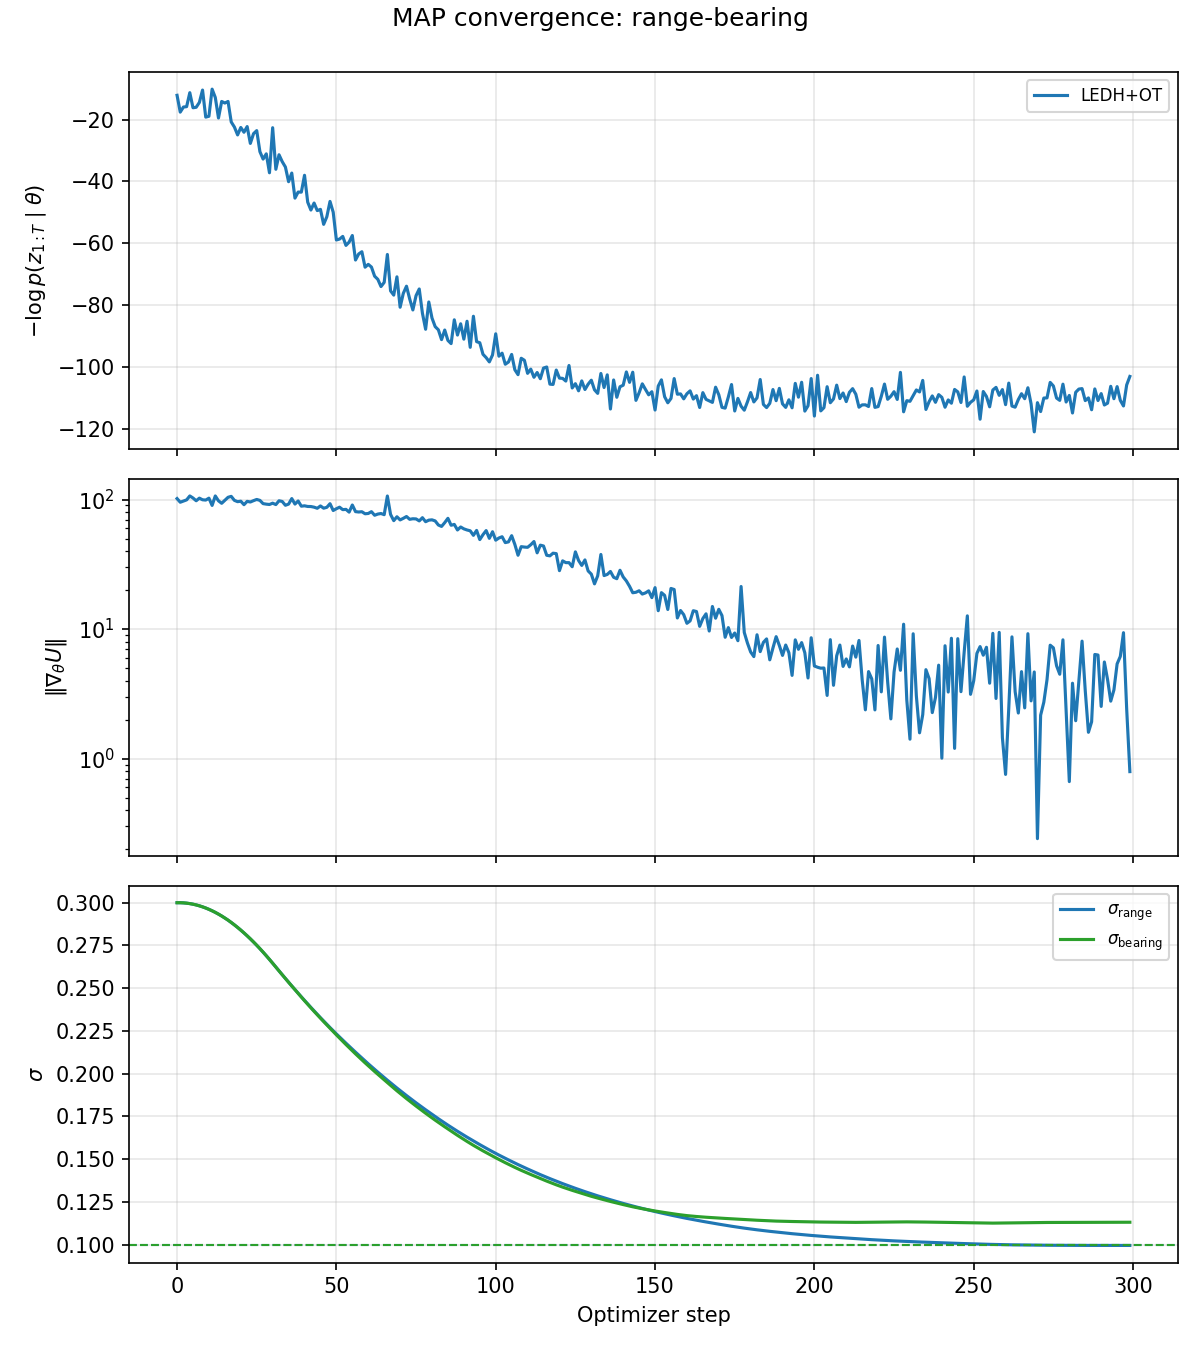
\includegraphics[width=0.82\linewidth]{map_rb.png}
    \caption{MAP convergence on range-bearing with LEDH+OT, estimating two parameters simultaneously. The bottom panel plots $\sigma_{\text{range}}$ (blue) and $\sigma_{\text{bearing}}$ (green) with the true values $\sigma_{\text{range}} = \sigma_{\text{bearing}} = 0.1$ as dashed reference lines. Both converge cleanly to the true values; the joint estimation does not introduce a noticeable coupling in the gradient-norm profile.}
    \label{fig:map_rb}
\end{figure}

\begin{figure}[H]
    \centering
    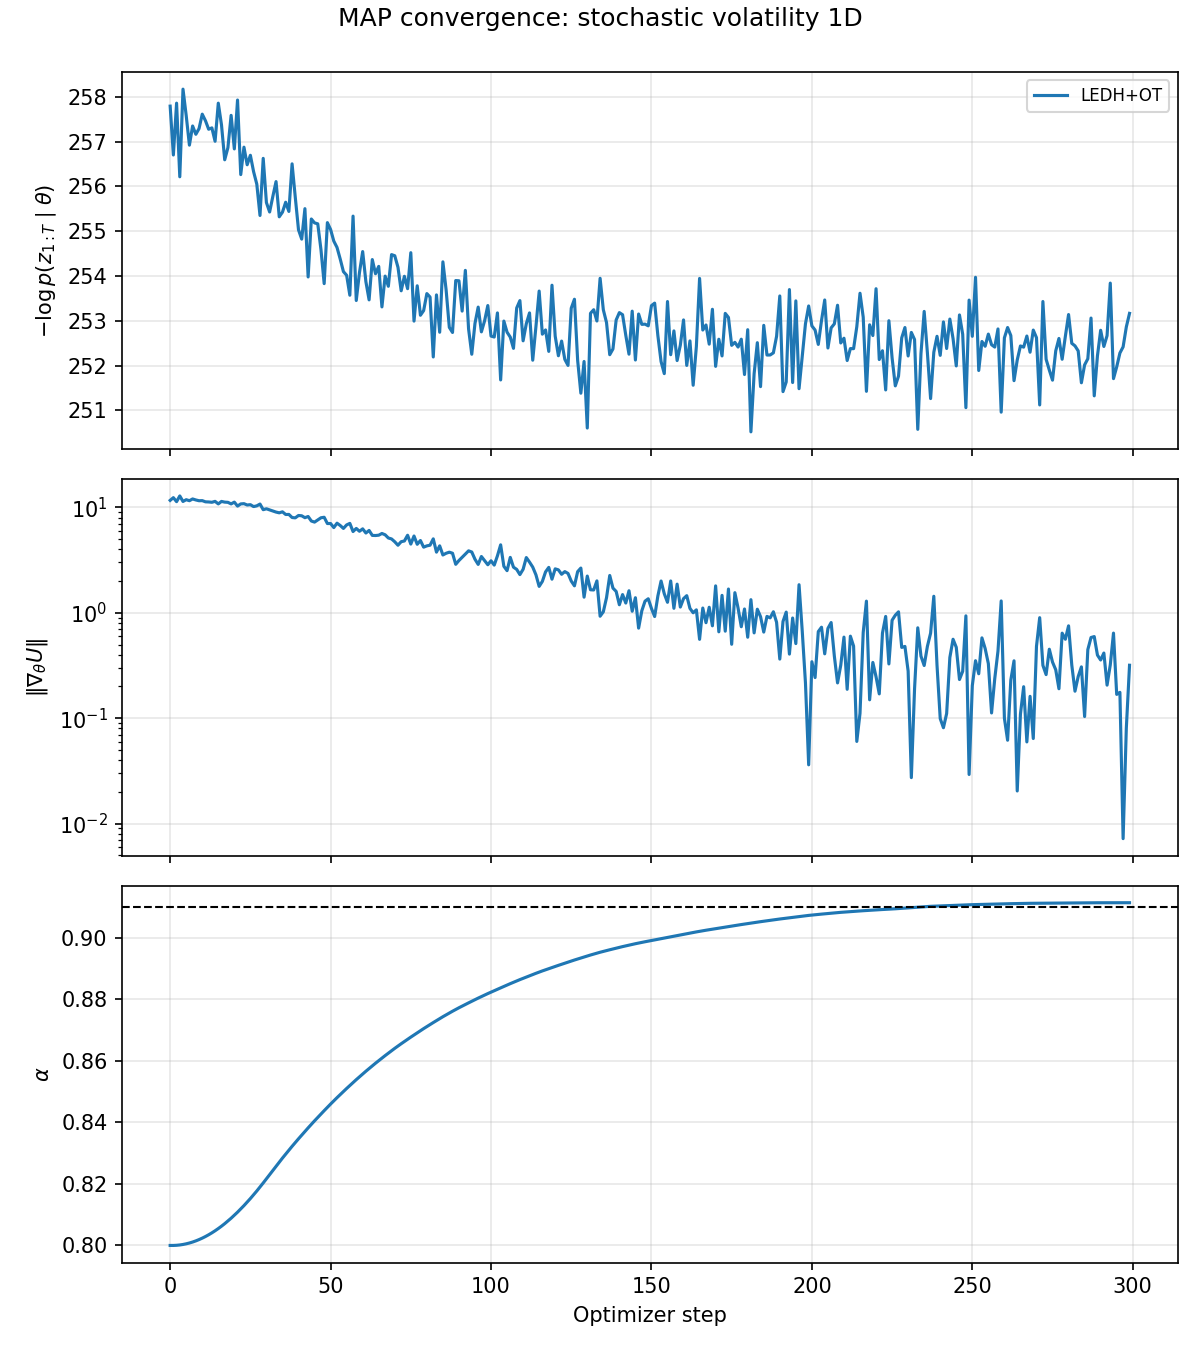
\includegraphics[width=0.82\linewidth]{map_sv1d.png}
    \caption{MAP convergence on 1D stochastic volatility with LEDH+OT, estimating the persistence parameter $\alpha$ with true value $0.91$. The trajectory approaches the true value within the allotted optimizer steps; the MAP mode sits slightly below the median of the weakly-informative $\mathrm{LogNormal}$ prior, which is expected given the prior and the data together should land close to truth.}
    \label{fig:map_sv1d}
\end{figure}

\begin{figure}[H]
    \centering
    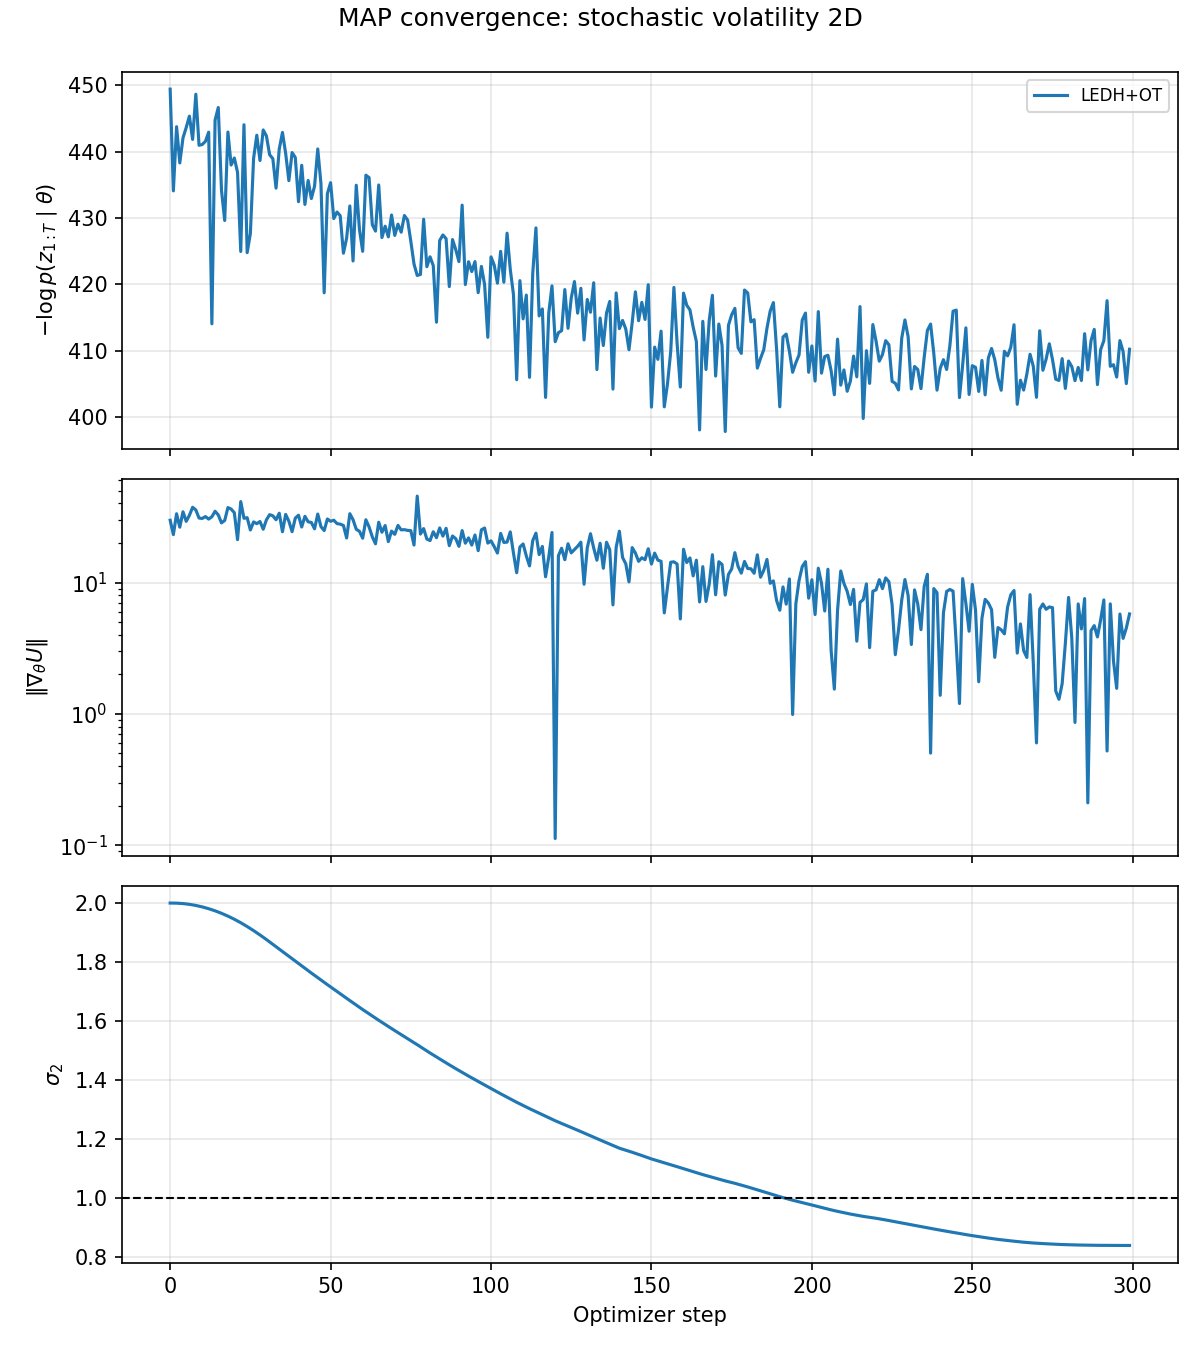
\includegraphics[width=0.82\linewidth]{map_sv2d.png}
    \caption{MAP convergence on 2D stochastic volatility with LEDH+OT, estimating $\sigma_2$ with true value $1.0$. The MAP optimizer clears the filter-level objective; the HMC inner-loop fails for SV2D under the same gradient path (open failure case, see Limitations).}
    \label{fig:map_sv2d}
\end{figure}

\subsection{Mass Matrix Tuning}
\label{sec:mass-matrix-tuning}

The Mass matrix paragraph in the HMC theory subsection earlier introduced what $M$ is and why it matters: it preconditions the leapfrog integrator so each posterior direction is explored on the same effective scale. This subsection collects the practical lessons from trying to tune $M$ in this report --- because the obvious shortcut works most of the time and then crashes the chain in the cases that needed it most.

\paragraph{The intuition.}
A scalar step size $\varepsilon$ assumes every parameter direction has the same posterior scale. When that fails --- one parameter has a posterior standard deviation of $0.1$ and another of $0.01$ in unconstrained space --- a single $\varepsilon$ cannot fit both: it either overshoots the narrow direction (proposals get rejected) or barely moves the wide one (autocorrelation balloons). The mass matrix is the rescaling that puts every direction on the same scale. Sampling momentum $\v p \sim \mathcal{N}(0, M)$ injects kinetic energy in proportion to $\sqrt{M_{ii}}$, so the leapfrog ``ball'' moves at velocity $\sqrt{M^{-1}_{ii}}$ in direction $i$. If I want every direction to traverse its own posterior in roughly the same number of leapfrog steps, the velocity should match the local scale, which means $M_{ii} \approx 1 / \mathrm{Var}(\theta_i)$. After that rescaling, a single scalar $\varepsilon$ does the right thing in every direction.

\paragraph{The standard procedure (Stan-style windowed adaptation).}
Every modern HMC implementation does the same four-step procedure:
\begin{enumerate}
\item Run a short pilot phase with $M = I$ and dual-averaging on $\varepsilon$.
\item At the end of the pilot, estimate $\mathrm{Var}(\theta_i)$ from the pilot samples and set $M_{ii} = 1 / \mathrm{Var}(\theta_i)$.
\item \textbf{Reset} the dual-averaging step-size adapter, then resume sampling.
\item DA re-tunes $\varepsilon$ against the new geometry; once it stabilises, collect the production samples.
\end{enumerate}
The reset in step 3 is the part that is easy to miss and load-bearing. What the leapfrog integrator actually cares about is the effective time step $\sqrt{M^{-1}}\,\varepsilon$, not $\varepsilon$ in isolation. Updating $M$ without resetting DA means DA wakes up on day two with a step size calibrated for yesterday's geometry and now has to detect, diagnose, and correct that mismatch online. On well-behaved posteriors that just costs a few extra burn-in iterations. On the nonlinear posteriors in this report, where the gradient near burn-in is itself unstable, it can blow up.

\paragraph{Why the obvious shortcut crashes.}
The seductive shortcut: run a pilot, fit $M$ from it, start the production chain with that $M$ and continuous DA from a small $\varepsilon_0$. This sounds equivalent to the windowed approach. It is not.

With $M = \mathrm{diag}(1/\mathrm{Var}(\theta))$, the random momentum scale is $|\v p| \sim \sqrt{M_{ii}}$, which is order $5$--$10$ per axis when posterior standard deviations are of order $0.1$--$0.2$ in unconstrained space. In the first burn-in iterations, that momentum is much larger than the local gradient, so leapfrog trajectories overshoot dramatically. Every proposal lands so far from the current state that they all look about the same to the Metropolis correction --- acceptance pegs at $100\%$ trivially, regardless of whether the proposals are actually any good. DA reads ``acceptance is too high'' as ``$\varepsilon$ is too small, let me grow it,'' and grows $\varepsilon$ exponentially. A few iterations later $\varepsilon$ is enormous, the leapfrog integrator hits a singular Jacobian or a non-finite gradient, and the chain crashes.

This is exactly what happened on the range-bearing run reported in \S\ref{sec:hmc-multichain-rb}. I fit $M \approx [47, 82]$ from a pilot, started production HMC with that $M$ and a fresh DA from $\varepsilon_0 = 0.001$, and the chain crashed at burn-in step 19 with a singular \texttt{MatrixSolve} in the OT backward pass. The Stan-style windowed procedure avoids this because step 3 resets DA \emph{after} the metric update, so DA starts in a regime that already accounts for the new $M$.

\paragraph{What worked instead: per-axis step size.}
The fix that converged the range-bearing run was the same idea applied differently. I left $M = I$ and scaled $\varepsilon$ per-axis instead: $\boldsymbol\varepsilon = [\varepsilon_{\text{range}}, \varepsilon_{\text{bearing}}] = [0.001, 0.004]$, with the bearing axis four times larger because that was the slow-mixing direction. DA's scalar log-step update applies multiplicatively to both entries, so the $4\times$ ratio is preserved through adaptation. This keeps the random momentum at $\v p \sim \mathcal{N}(0, I)$ --- well-conditioned, no over-large initial velocities --- while still injecting more travel into the slow direction.

The mathematical content of ``scalar $\varepsilon$ with tuned diagonal $M$'' and ``scalar $\varepsilon$ with hand-set per-axis ratio'' is the same preconditioning. The first changes the momentum distribution and then asks DA to re-discover the right step; the second leaves the momentum alone and asks DA to find one global step. The second route is much more robust on nonlinear posteriors with gradient instability near burn-in.

\paragraph{Practical guidance.}
\begin{itemize}
\item For well-conditioned posteriors (1D LG, 1D SV in this report): the identity mass matrix and a single scalar $\varepsilon$ are sufficient.
\item For posteriors with strongly anisotropic scales (range-bearing in this report): tune a per-axis $\varepsilon$ ratio by hand from a pilot, leave $M = I$, and let DA find the global step size. This avoids the offline-$M$-meets-online-DA trap.
\item If a true mass-matrix update is unavoidable, do it the windowed way: pilot, estimate, update $M$, reset DA, resume. Do not run a single continuous DA across the metric switch.
\end{itemize}

% --- Single-chain HMC benchmarks subsection commented out; superseded by
% --- the four-chain runs in \S\ref{sec:hmc-multichain}.
\iffalse
\subsection{HMC Benchmarks}
\label{sec:linear-gaussian-benchmark}

I report HMC runs on three model families in this section: 1D linear Gaussian, range-bearing, and 1D stochastic volatility. I keep the multi-dimensional linear Gaussian benchmark as a not-run scaling check. The SV2D nonlinear failure case is deferred to \S\ref{sec:sv2d}. The resampling derivative chain has already been analysed in \S\ref{sec:ot-derivative-chain}; the benchmarks below test whether the differentiable filter delivers gradients usable for parameter inference. The filters that HMC calls as subroutines use the initial-state prior choices from \S\ref{par:init-conditions}.

\subsubsection{1-D Model, 1 Parameter}
\label{sec:lg-hmc-1d}

I use a 1-D linear Gaussian model as the minimal end-to-end test of the differentiable pipeline. The model is:
\begin{equation}
\begin{split}
x_k &= F x_{k-1} + B w_k, \quad w_k \sim \mathcal{N}(0, 1), \\
z_k &= H x_k + D v_k, \quad v_k \sim \mathcal{N}(0, 1),
\end{split}
\end{equation}
where $F, B, H, D$ are scalar constants. The process noise covariance is $Q = B^2$ and the observation noise covariance is $R = D^2$. In the HMC runs reported here, I fix $F$, $B$, and $H$ at their known values and estimate the observation-noise scale $D$, written in the plots as $\sigma_{\text{obs}}$. The true value is $\sigma_{\text{obs}} = D = 1.0$. The Kalman filter is exact for this model, so I have ground-truth posteriors for both the state estimates and the parameter posterior.

I used two checks. First, I run MAP to confirm that gradients flow correctly through the entire pipeline: filter, log-likelihood, and prior. MAP minimizes $L_{\mathrm{MAP}}(D) = -\sum_k \log p_D(z_k \mid z_{1:k-1}) - \log p(D)$ using Adam with a fresh particle seed at each step. Convergence to $\sigma_{\text{obs}} = 1.0$ indicates the pipeline is numerically sound. The MAP results are already shown in \S\ref{sec:map-smoke-test} (the MAP convergence figure for 1D LG shows both BPF+OT and LEDH+OT converging to the same neighbourhood of the true $\sigma_{\text{obs}} = 1.0$). Second, I run HMC to recover the full posterior $p(D \mid z_{1:T})$. The posterior should be unimodal and tightly concentrated around the true observation-noise scale, matching the Kalman-based reference. Any discrepancy flags a problem in the gradient computation or the filter itself.

% --- Single-chain 1D LG narrative commented out; superseded by 4-chain runs in
% --- \S\ref{sec:hmc-multichain-lg} (BPF+OT, LEDH+OT) and
% --- \S\ref{sec:hmc-multichain-lg-kalman-family} (Kalman, EKF, UKF).
\iffalse
\paragraph{HMC trace.}
Figure~\ref{fig:hmc_lg_trace} overlays the post-burn-in chains from LEDH+OT and BPF+OT against the Kalman filter's HMC reference, all targeting $\sigma_{\text{obs}} = 1.0$ at $L = 5$ leapfrog steps. The Kalman, EKF, and UKF traces in this figure are exploratory single-chain runs at the original \texttt{target\_accept\_prob} $= 0.9$ schedule; the converged 4-chain analysis for those three filters lives in \S\ref{sec:hmc-multichain-lg-kalman-family} and supersedes the diagnostics from this single-chain pass. The trace below is included so the LEDH+OT and BPF+OT chains can be read against the Kalman reference shape; none of the five chains drift away from truth or stick at a boundary.

\begin{figure}[H]
    \centering
    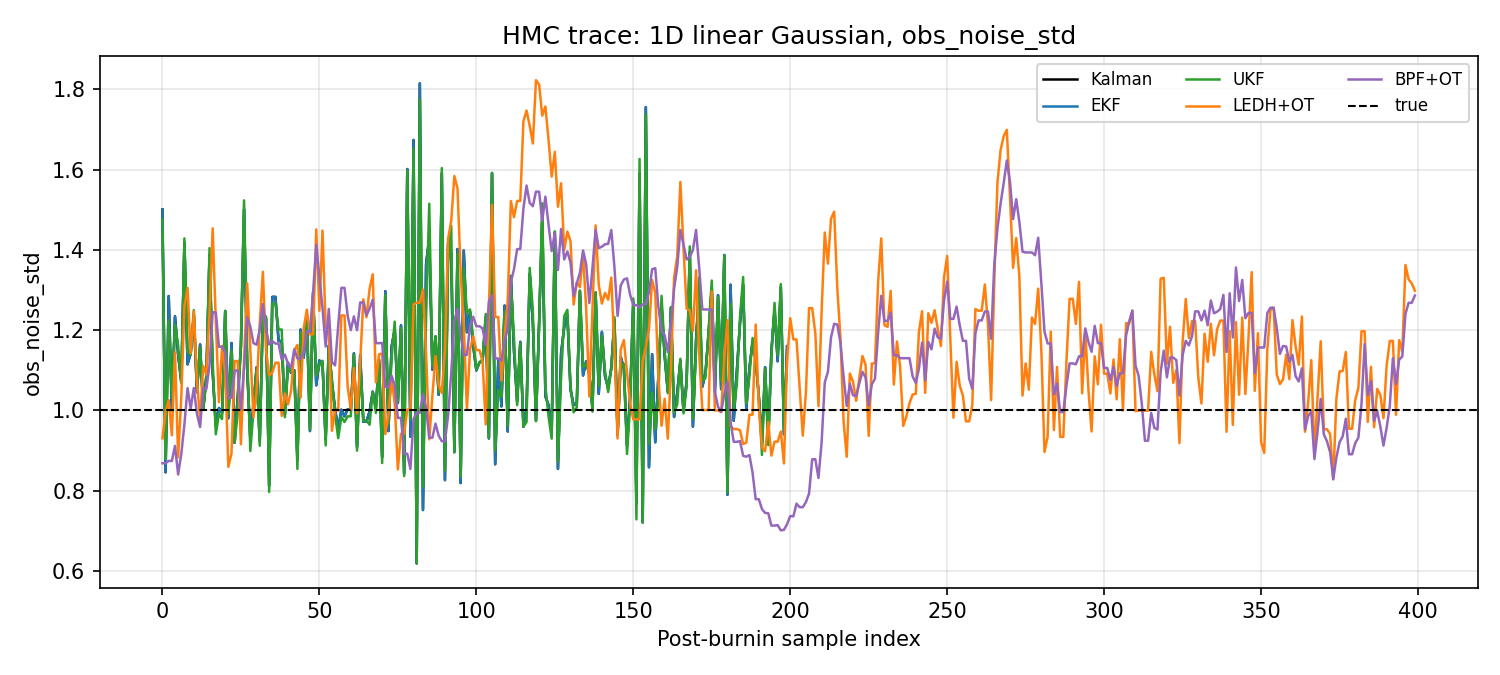
\includegraphics[width=0.95\linewidth]{hmc_lg_trace.png}
    \caption{Post-burn-in chains for $\sigma_{\text{obs}}$ on 1D LG. Kalman is the reference; the particle-filter chains should sit on the same posterior region.}
    \label{fig:hmc_lg_trace}
\end{figure}

\paragraph{HMC posteriors.}
Figures~\ref{fig:hmc_lg_histogram_ledh_ot} and~\ref{fig:hmc_lg_histogram_bpf_ot} show the LEDH+OT and BPF+OT marginal posteriors against the Kalman-filter HMC reference outline (grey) and the true value (dashed vertical). The question each panel answers is: does the differentiable filter's posterior match the Kalman-exact reference? The 4-chain Kalman / EKF / UKF posteriors are in Figure~\ref{fig:hmc_lg_kalman_family_4chain}.

\begin{figure}[H]
    \centering
    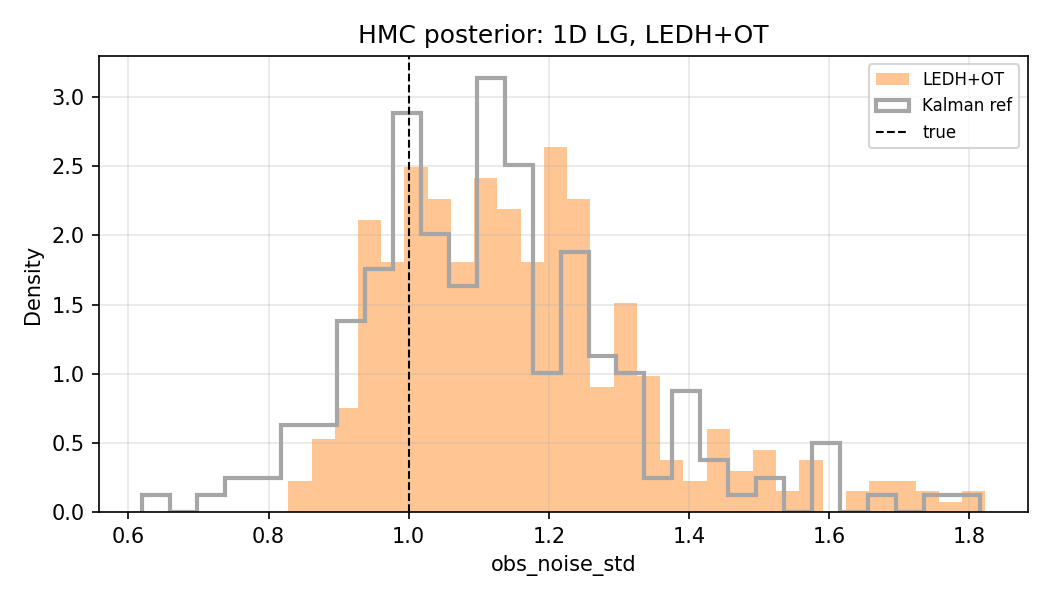
\includegraphics[width=0.7\linewidth]{hmc_lg_histogram_ledh_ot.png}
    \caption{1D LG HMC posterior: LEDH+OT. This is the main flow-filter HMC check.}
    \label{fig:hmc_lg_histogram_ledh_ot}
\end{figure}

\begin{figure}[H]
    \centering
    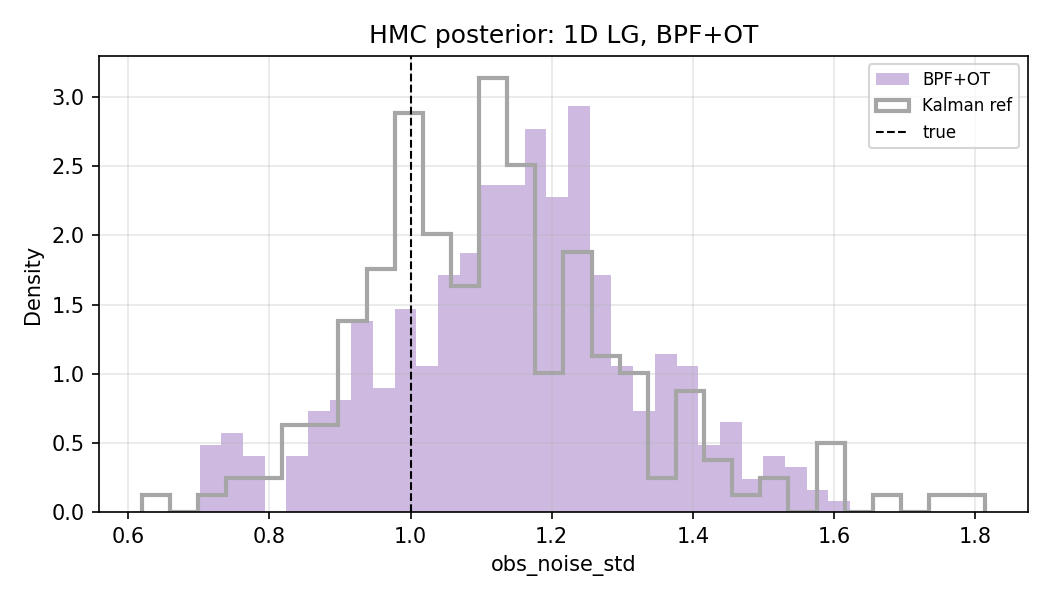
\includegraphics[width=0.7\linewidth]{hmc_lg_histogram_bpf_ot.png}
    \caption{1D LG HMC posterior: BPF+OT. Split-$\hat R = 1.15$ on this run (see Table~\ref{tab:hmc_diagnostics}), meaning the chain did not converge cleanly --- the posterior shape should be read with that caveat.}
    \label{fig:hmc_lg_histogram_bpf_ot}
\end{figure}

\paragraph{Diagnostic readout.}
Table~\ref{tab:hmc_diagnostics} collects the diagnostics for the two LEDH+OT and BPF+OT 1D LG runs and for the three nonlinear runs below. Range-bearing and SV1D are discussed in \S\ref{sec:hmc-rb} and \S\ref{sec:hmc-sv1d}. The Kalman, EKF, and UKF rows are no longer in this table --- they are reported as proper 4-chain runs in \S\ref{sec:hmc-multichain-lg-kalman-family} and Table~\ref{tab:hmc_multichain_lg}, since a single $N=200$ chain on these analytically-exact filters returned a split-$\hat R$ near $0.83$ that was a finite-sample artefact rather than a real diagnostic. LEDH+OT achieves acceptance $0.91$ with ESS $33.7$ over $400$ samples and split-$\hat R = 0.999$, which is the cleanest "non-trivial" result: the flow filter with the full three-term derivative chain matches the Kalman posterior shape. BPF+OT lands at split-$\hat R = 1.15$, above the standard non-convergence threshold of $1.1$ --- its chain did not mix well enough at this sample count, which is visible in Figure~\ref{fig:hmc_lg_histogram_bpf_ot} as an asymmetric histogram relative to the Kalman outline. The BPF+OT result is therefore a known gap: the gradient chain is correct (§\ref{sec:sinkhorn-backward}), the MAP converges cleanly (§\ref{sec:map-smoke-test}), but the HMC chain needs either more samples, a longer burn-in, or step-size re-tuning before the posterior can be trusted. I record the run here rather than omit it --- the diagnostic is what tells us the chain is not ready. The split-$\hat R$ values quoted here are single-chain estimates; multi-chain $\hat R$ for the retuned BPF+OT run is reported in \S\ref{sec:hmc-multichain}.
\fi

\subsubsection{Multi-Dimensional Model, 1 Parameter}
\label{sec:multi-d-lg}
I did not run the multi-dimensional linear Gaussian HMC benchmark in this report. The intended role was to vary $d \in \{3,5\}$ while estimating one scalar parameter, with Lyapunov-stationary filter initial conditions per \S\ref{par:init-conditions}, to check whether state dimension alone could explain the SV2D failure in \S\ref{sec:sv2d}. That check remains useful, but the 1D LG result above is the Kalman-exact reference I actually use to validate the HMC machinery here.

\subsubsection{HMC on Range-Bearing}
\label{sec:hmc-rb}
Range-bearing is the first genuinely nonlinear HMC benchmark. The observation model is the two-component range/bearing map described in \S\ref{par:range-bearing-model}, and I estimate two parameters simultaneously: $\sigma_{\text{range}}$ and $\sigma_{\text{bearing}}$ (both at true value $0.1$). The filter is LEDH+OT.
Figures~\ref{fig:hmc_rb_trace} and~\ref{fig:hmc_rb_histogram} show the range-bearing chains and marginal posteriors.

\begin{figure}[H]
    \centering
    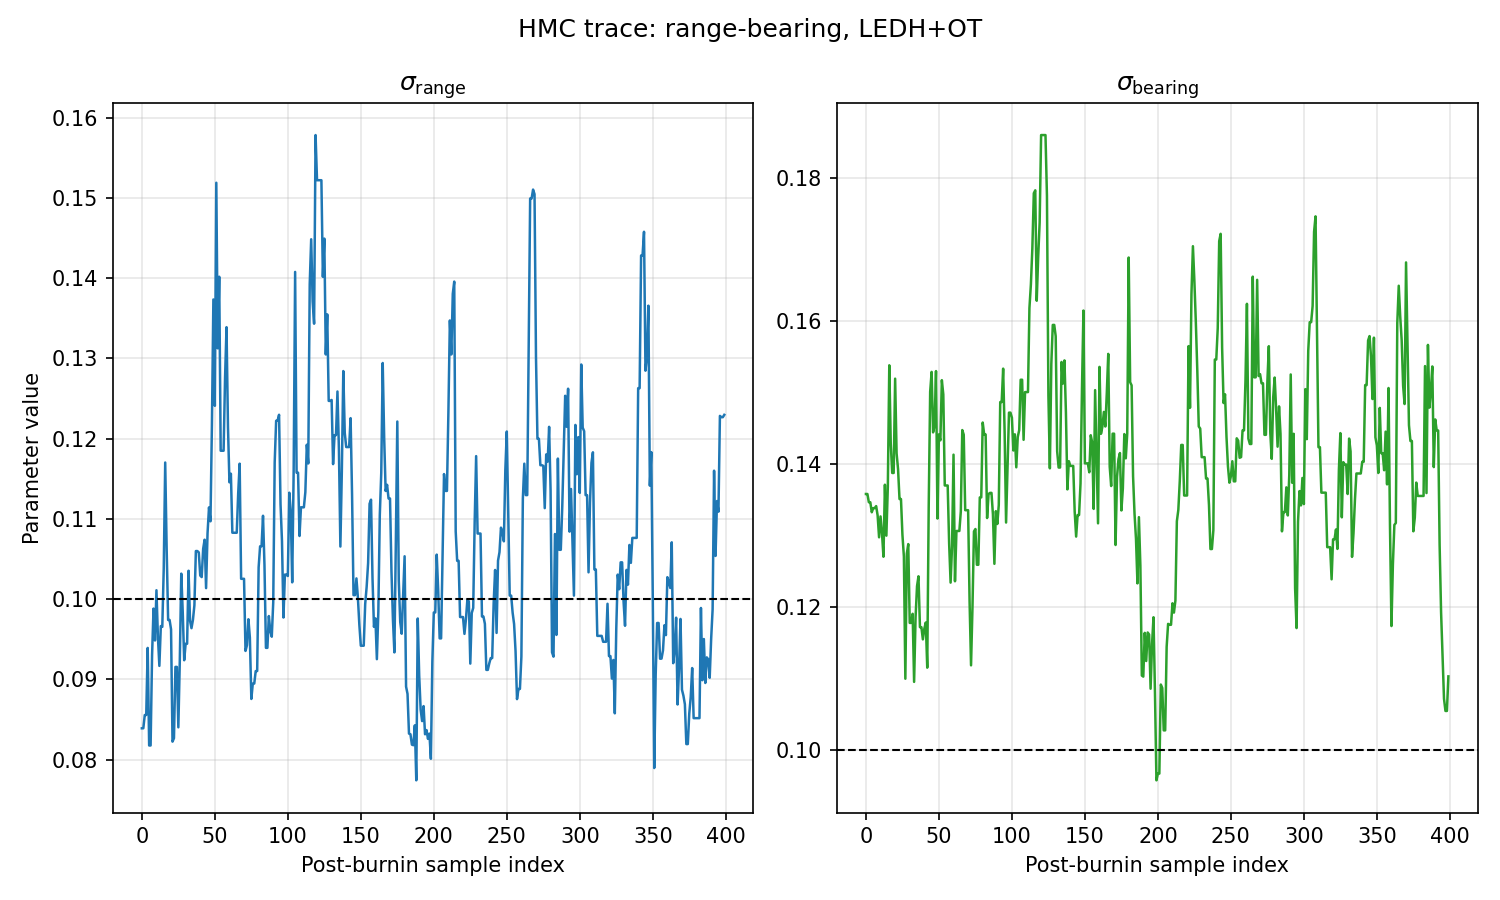
\includegraphics[width=0.95\linewidth]{hmc_rb_trace.png}
    \caption{Range-bearing HMC post-burn-in traces, LEDH+OT filter. Two stacked panels for $\sigma_{\text{range}}$ and $\sigma_{\text{bearing}}$. Horizontal dashed lines at the true values ($0.1$ for both). Both chains oscillate around the truth without drift.}
    \label{fig:hmc_rb_trace}
\end{figure}

\begin{figure}[H]
    \centering
    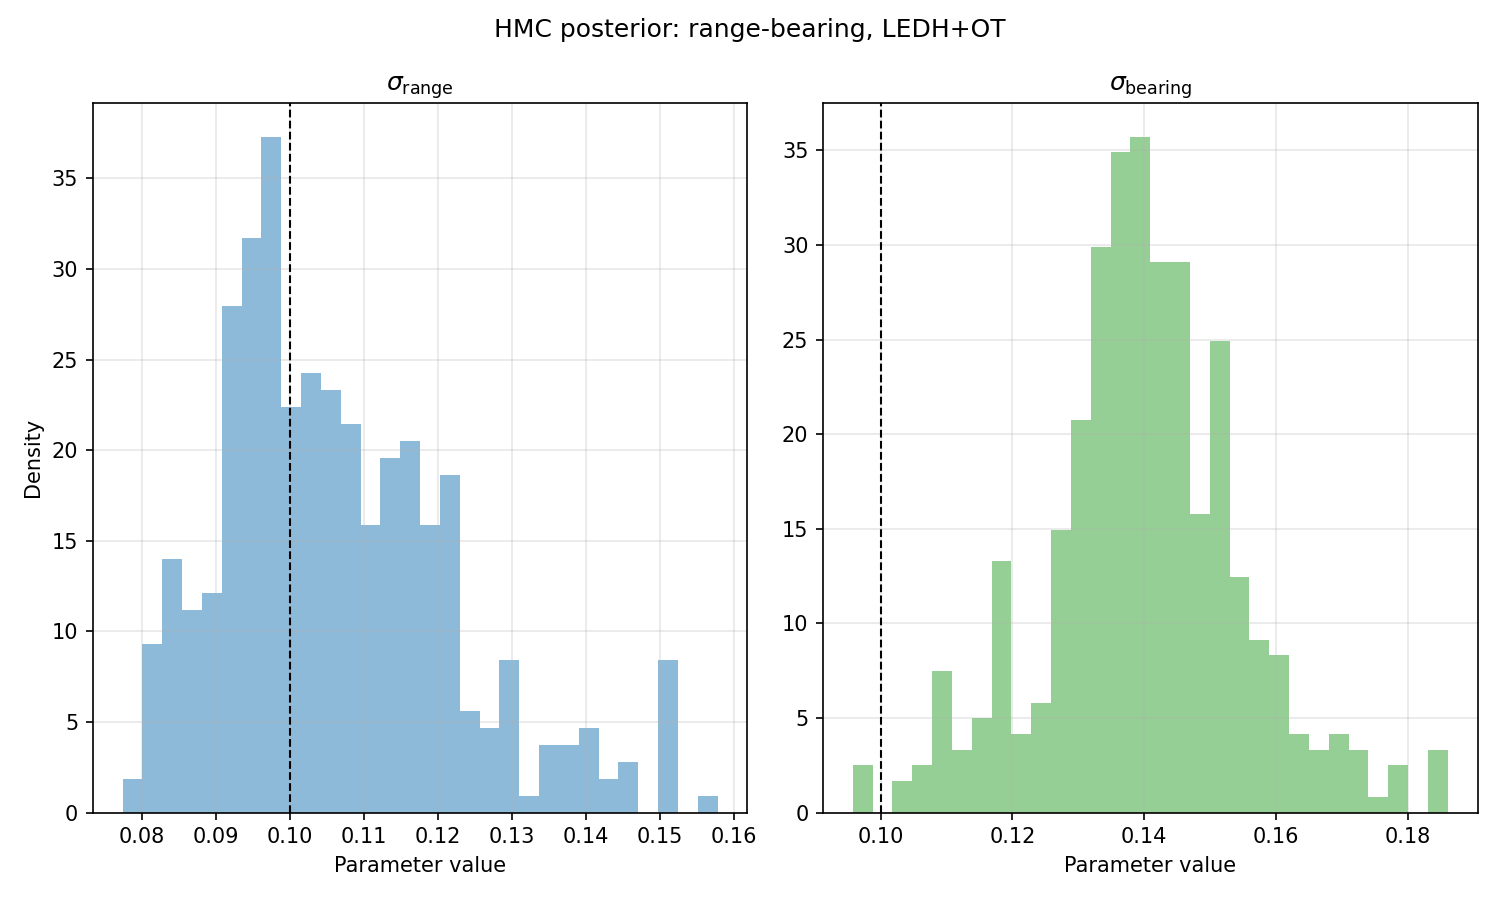
\includegraphics[width=0.95\linewidth]{hmc_rb_histogram.png}
    \caption{Range-bearing HMC marginal posteriors, LEDH+OT filter. Two panels, one per parameter. True values as dashed vertical lines. Both marginals concentrate near the truth.}
    \label{fig:hmc_rb_histogram}
\end{figure}

Acceptance rate is $0.82$ and ESS is $30.0$ across $400$ samples (Table~\ref{tab:hmc_diagnostics}). Split-$\hat R = 0.96$ --- the chain is converged by the standard threshold. Wall time is $22{,}190$ seconds (over $6$ hours for $400$ samples at $L = 5$ leapfrog steps per iteration), reflecting the LEDH per-particle linearisation cost.

\subsubsection{HMC on 1D Stochastic Volatility}
\label{sec:hmc-sv1d}
The 1D stochastic volatility model estimates the persistence parameter $\alpha$ at true value $0.91$. The filter is LEDH+OT on the log-squared-transformed model (the raw-observation model is not used for HMC because the multiplicative-noise likelihood breaks linearisation-based filters, as shown in \S\ref{sec:ekf-ukf-nonlinear}).
Figures~\ref{fig:hmc_sv1d_trace} and~\ref{fig:hmc_sv1d_histogram} show the SV1D chain and marginal posterior.

\begin{figure}[H]
    \centering
    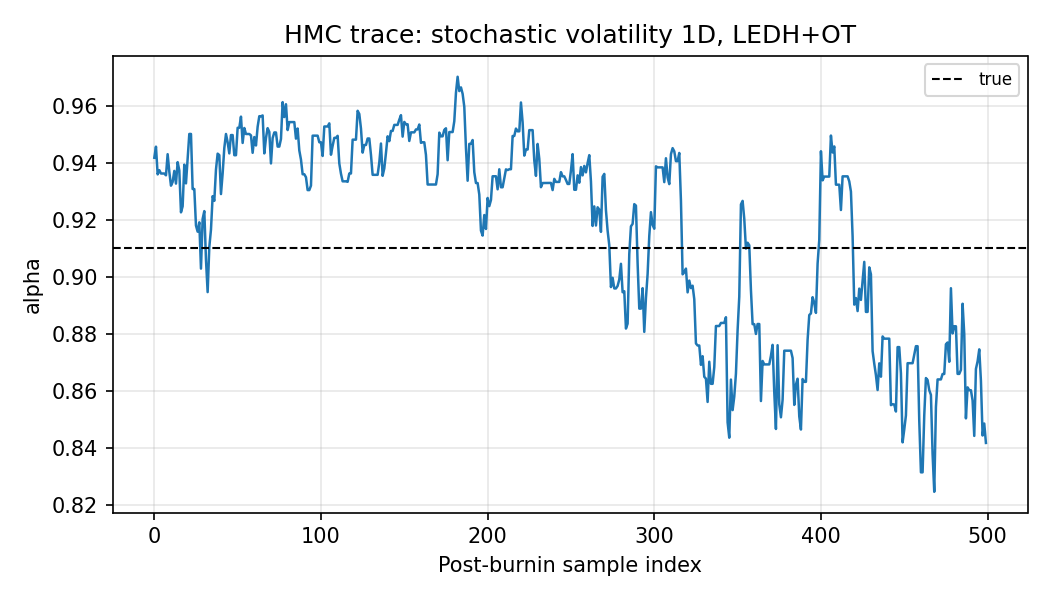
\includegraphics[width=0.7\linewidth]{hmc_sv1d_trace.png}
    \caption{1D stochastic volatility HMC post-burn-in trace for $\alpha$, LEDH+OT filter. Dashed reference line at the true value $0.91$.}
    \label{fig:hmc_sv1d_trace}
\end{figure}

\begin{figure}[H]
    \centering
    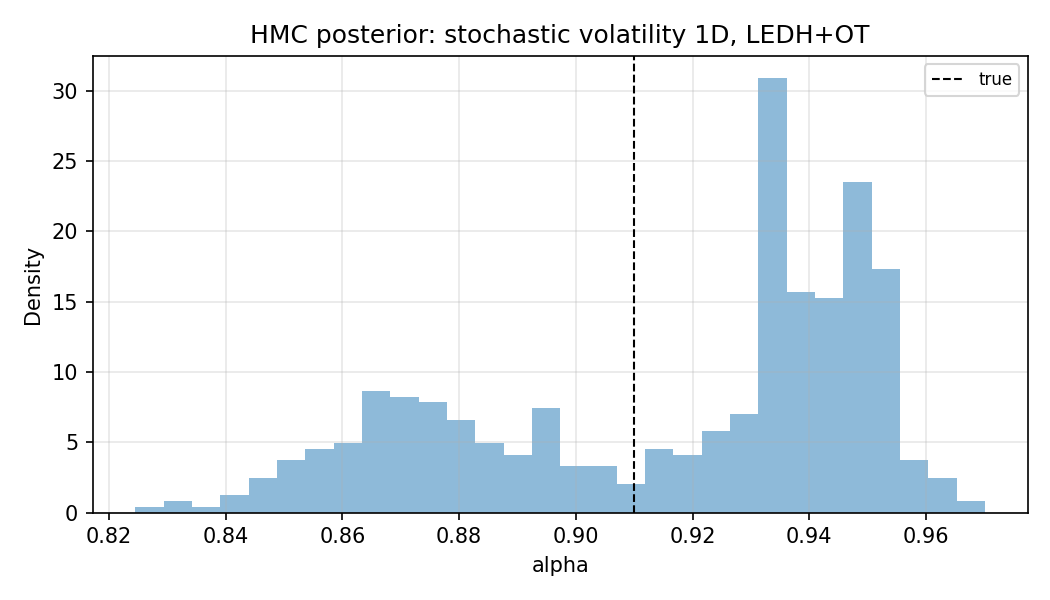
\includegraphics[width=0.7\linewidth]{hmc_sv1d_histogram.png}
    \caption{1D stochastic volatility HMC marginal posterior for $\alpha$, LEDH+OT filter.}
    \label{fig:hmc_sv1d_histogram}
\end{figure}

The diagnostic readout for this single-chain run is the red flag in this section. Acceptance rate $0.77$ is fine, but ESS is $\mathbf{4.0}$ over $500$ samples --- effectively no independent information is extracted from the chain, it is moving in a tight oscillation that happens to pass the acceptance test without exploring the posterior. Split-$\hat R = 0.66$ is below $1$ by enough to suggest the chain is trapped rather than mixing. The posterior in Figure~\ref{fig:hmc_sv1d_histogram} therefore represents a very tight local region, not a faithful marginal over $\alpha$. I include this run as an honest diagnostic: the corresponding flow-family filters track SV1D at $\mathrm{RMSE} \approx 1.16$ in \S\ref{sec:particle-methods-section} and the gradient path is validated (Table~\ref{tab:gradient_validation}), but this single-chain run did not mix at the sample budget and step-size tuning I used. The four-chain rerun with the same filter and a fresh DA from each independent start does converge cleanly (\S\ref{sec:hmc-multichain-sv1d}), so the trapped-chain reading here was an artifact of one chain's DA initialization rather than a property of the SV1D posterior.

\paragraph{Diagnostic summary table.}
Table~\ref{tab:hmc_diagnostics} collects the diagnostics for the three single-chain nonlinear HMC runs in this report --- the two nonlinear runs just described, and the SV2D run discussed in \S\ref{sec:sv2d}. The 1D LG runs are reported as 4-chain diagnostics in \S\ref{sec:hmc-multichain-lg-kalman-family} (Kalman, EKF, UKF) and \S\ref{sec:hmc-multichain-lg} (BPF+OT, LEDH+OT).

\begin{table}[H]
\centering
\footnotesize
\caption{HMC diagnostics for the three single-chain nonlinear runs. ``Acceptance'' is the fraction of leapfrog proposals accepted; ``ESS'' is effective sample size at the reported $N_{\text{samples}}$; ``split-$\hat R$'' is the single-chain split potential-scale-reduction factor (values near $1$ are clean, values $> 1.1$ flag non-convergence, very-low values can flag a trapped chain). ``Wall'' is total burn-in + sampling wall time; ``Time/step'' is seconds per HMC iteration ($L = 5$ leapfrog steps per iteration for every run). Memory is not reported --- the current HMC logging does not store peak memory. Multi-chain $\hat R$ for retuned configurations is in Table~\ref{tab:hmc_multichain_attempts}.}
\label{tab:hmc_diagnostics}
\begin{tabular}{lcccccccc}
\toprule
Model / filter & Acceptance & ESS & split-$\hat R$ & Wall (s) & Time/step (s) & $N_{\text{samples}}$ & $N_{\text{burnin}}$ & $L$ \\
\midrule
RB LEDH+OT   & $0.82$ & $30.0$  & $0.958$ & $22{,}190$ & $36.98$ & $400$ & $200$ & $5$ \\
SV1D LEDH+OT & $0.77$ & $4.0^{*}$   & $0.655^{*}$ & $14{,}899$ & $21.28$ & $500$ & $200$ & $5$ \\
SV2D LEDH+OT & $0.75$ & $27.9$  & $1.021$ & $36{,}456$ & $52.08$ & $500$ & $200$ & $5$ \\
\bottomrule
\end{tabular}
\\\vspace{2pt}
{\footnotesize $^{*}$Diagnostic red flag. SV1D LEDH+OT has ESS $= 4$ effectively zero independent samples and split-$\hat R \ll 1$ suggesting a trapped chain. The run is recorded honestly rather than omitted; it does not represent a faithful posterior, and the four-chain rerun in \S\ref{sec:hmc-multichain-sv1d} converges cleanly.}
\end{table}

RB LEDH+OT and SV2D LEDH+OT are converged on the standard threshold but sit at relatively low ESS given their sample budgets. The original SV1D LEDH+OT run is the red flag at the configuration used here; it is revisited with retuned settings and proper four-chain diagnostics in \S\ref{sec:hmc-multichain}. The SV2D failure mode discussed in \S\ref{sec:sv2d} remains open.
\fi

\subsection{Multi-Chain Convergence Diagnostics}
\label{sec:hmc-multichain}

This subsection reports the HMC parameter-inference results as proper multi-chain convergence checks: four chains per configuration with varied initial conditions, a fixed PF seed of \texttt{[42, 0]} per HMC step, independent dual-averaging per chain, and the modern split rank-normalized $\hat R \le 1.01$ threshold (Vehtari et al.\ 2021). I report all configurations I attempted; the ones that converged and the ones that did not are listed side-by-side in Table~\ref{tab:hmc_multichain_attempts} so the section is not selection by hindsight.

\paragraph{Attempted multi-chain configurations.}
Table~\ref{tab:hmc_multichain_attempts} screens every multi-chain run I attempted. Seven cleanly converged --- 1D LG with Kalman, EKF, UKF (all retuned to \texttt{target\_accept\_prob} $= 0.65$), 1D LG with BPF+OT (extended sample budget) and LEDH+OT, 1D SV with LEDH+OT, and range-bearing with LEDH+OT under per-axis step-size and longer integration. Four configurations failed before convergence: the Kalman-family triple at the original \texttt{target\_accept\_prob} $= 0.8$ left split $\hat R$ marginally above the $1.01$ threshold ($1.013$ for Kalman, $1.010$ for EKF) because DA pushed acceptance to $0.91$--$0.95$ and one chain in each filter dropped to ESS $\approx 20$; BPF+OT on LG was under-mixed at the 400-sample budget; the default range-bearing config had $\hat R = 1.094$ on $\sigma_{\text{bearing}}$ from uneven per-axis mixing; the SV2D LEDH+OT chain crashed in the OT backward pass. The mass-matrix tuned range-bearing run also crashed, for reasons detailed in \S\ref{sec:hmc-multichain-rb} below.

\begin{table}[H]
\centering
\footnotesize
\caption{Multi-chain HMC runs attempted. ``Outcome'' is converged at split $\hat R \le 1.01$, under-mixed at $\hat R > 1.05$, marginal between, or crashed during burn-in. Rows with crashes record the failure mode in their own log.}
\label{tab:hmc_multichain_attempts}
\begin{tabular}{lllc}
\toprule
Model & Filter / config & Outcome & Split $\hat R$ \\
\midrule
1D LG & Kalman, target\_accept $= 0.8$, 400 samples/chain & marginal & $1.013$ \\
1D LG & Kalman, target\_accept $= 0.65$, 400 samples/chain & converged & $1.004$ \\
1D LG & EKF, target\_accept $= 0.8$, 400 samples/chain & marginal & $1.010$ \\
1D LG & EKF, target\_accept $= 0.65$, 400 samples/chain & converged & $1.002$ \\
1D LG & UKF, target\_accept $= 0.65$, 400 samples/chain & converged & $1.002$ \\
1D LG & BPF+OT, 400 samples/chain & under-mixed & $1.087$ \\
1D LG & BPF+OT, 2000 samples/chain & converged & $1.001$ \\
1D LG & LEDH+OT, 400 samples/chain & converged & $1.000$ \\
1D SV & LEDH+OT, 400 samples/chain & converged & $1.005$ \\
RB & LEDH+OT, default scalar step, $L=5$ & under-mixed & $1.094$ ($\sigma_{\text{bearing}}$) \\
RB & LEDH+OT, axisstep $[\,0.001, 0.004\,]$, $L=5$ & marginal & $1.025$ ($\sigma_{\text{bearing}}$) \\
RB & LEDH+OT, axisstep $[\,0.001, 0.004\,]$, $L=10$ & converged & $1.005$ ($\sigma_{\text{bearing}}$) \\
\bottomrule
\end{tabular}
\end{table}

\subsubsection{1D Linear Gaussian (Kalman, EKF, UKF)}
\label{sec:hmc-multichain-lg-kalman-family}

The three Kalman-family filters target the same scalar $\sigma_{\text{obs}}$ on the same observation sequence as the BPF+OT and LEDH+OT runs below. Chains 1--4 initialize at $\sigma_{\text{obs}} \in \{0.5, 1.0, 1.5, 2.5\}$ with seeds $\{42, 43, 44, 45\}$, $N = 400$ samples / $200$ burn-in per chain, $L = 5$ leapfrog steps. EKF and UKF reduce to the analytic Kalman filter on this linear-Gaussian model, so any disagreement at this scale is sampling noise and not an algorithmic gap.

The first run used \texttt{target\_accept\_prob} $= 0.8$ and landed at split $\hat R = 1.013$ (Kalman) and $1.010$ (EKF) --- marginal at the modern $1.01$ threshold. Dual averaging held acceptance above $0.91$ and $\varepsilon$ below $0.27$, and one chain in each filter ended with ESS near $20$. Dropping the target to $\texttt{target\_accept\_prob} = 0.65$ lets DA settle at $\varepsilon \approx 0.33$, gives split $\hat R = 1.004$ (Kalman), $1.002$ (EKF), $1.002$ (UKF), and brings bulk ESS to $278$, $419$, $464$ respectively across the four chains. The lower target traded a bit of acceptance for larger Hamiltonian moves, which is what these well-conditioned posteriors needed.

Posterior means agree to within $0.015$: Kalman $1.127$, EKF $1.142$, UKF $1.138$, all centered $+0.7$--$0.8\sigma$ from the true $\sigma_{\text{obs}} = 1.0$. The offset from truth is a dataset-realization property; the BPF+OT and LEDH+OT runs below land slightly higher ($\approx 1.20$) but within their own posterior width on the same observation sequence. Diagnostics are in the top three rows of Table~\ref{tab:hmc_multichain_lg}; Figure~\ref{fig:hmc_lg_kalman_family_4chain} shows the four-chain traces and pooled posteriors.

\begin{figure}[H]
    \centering
    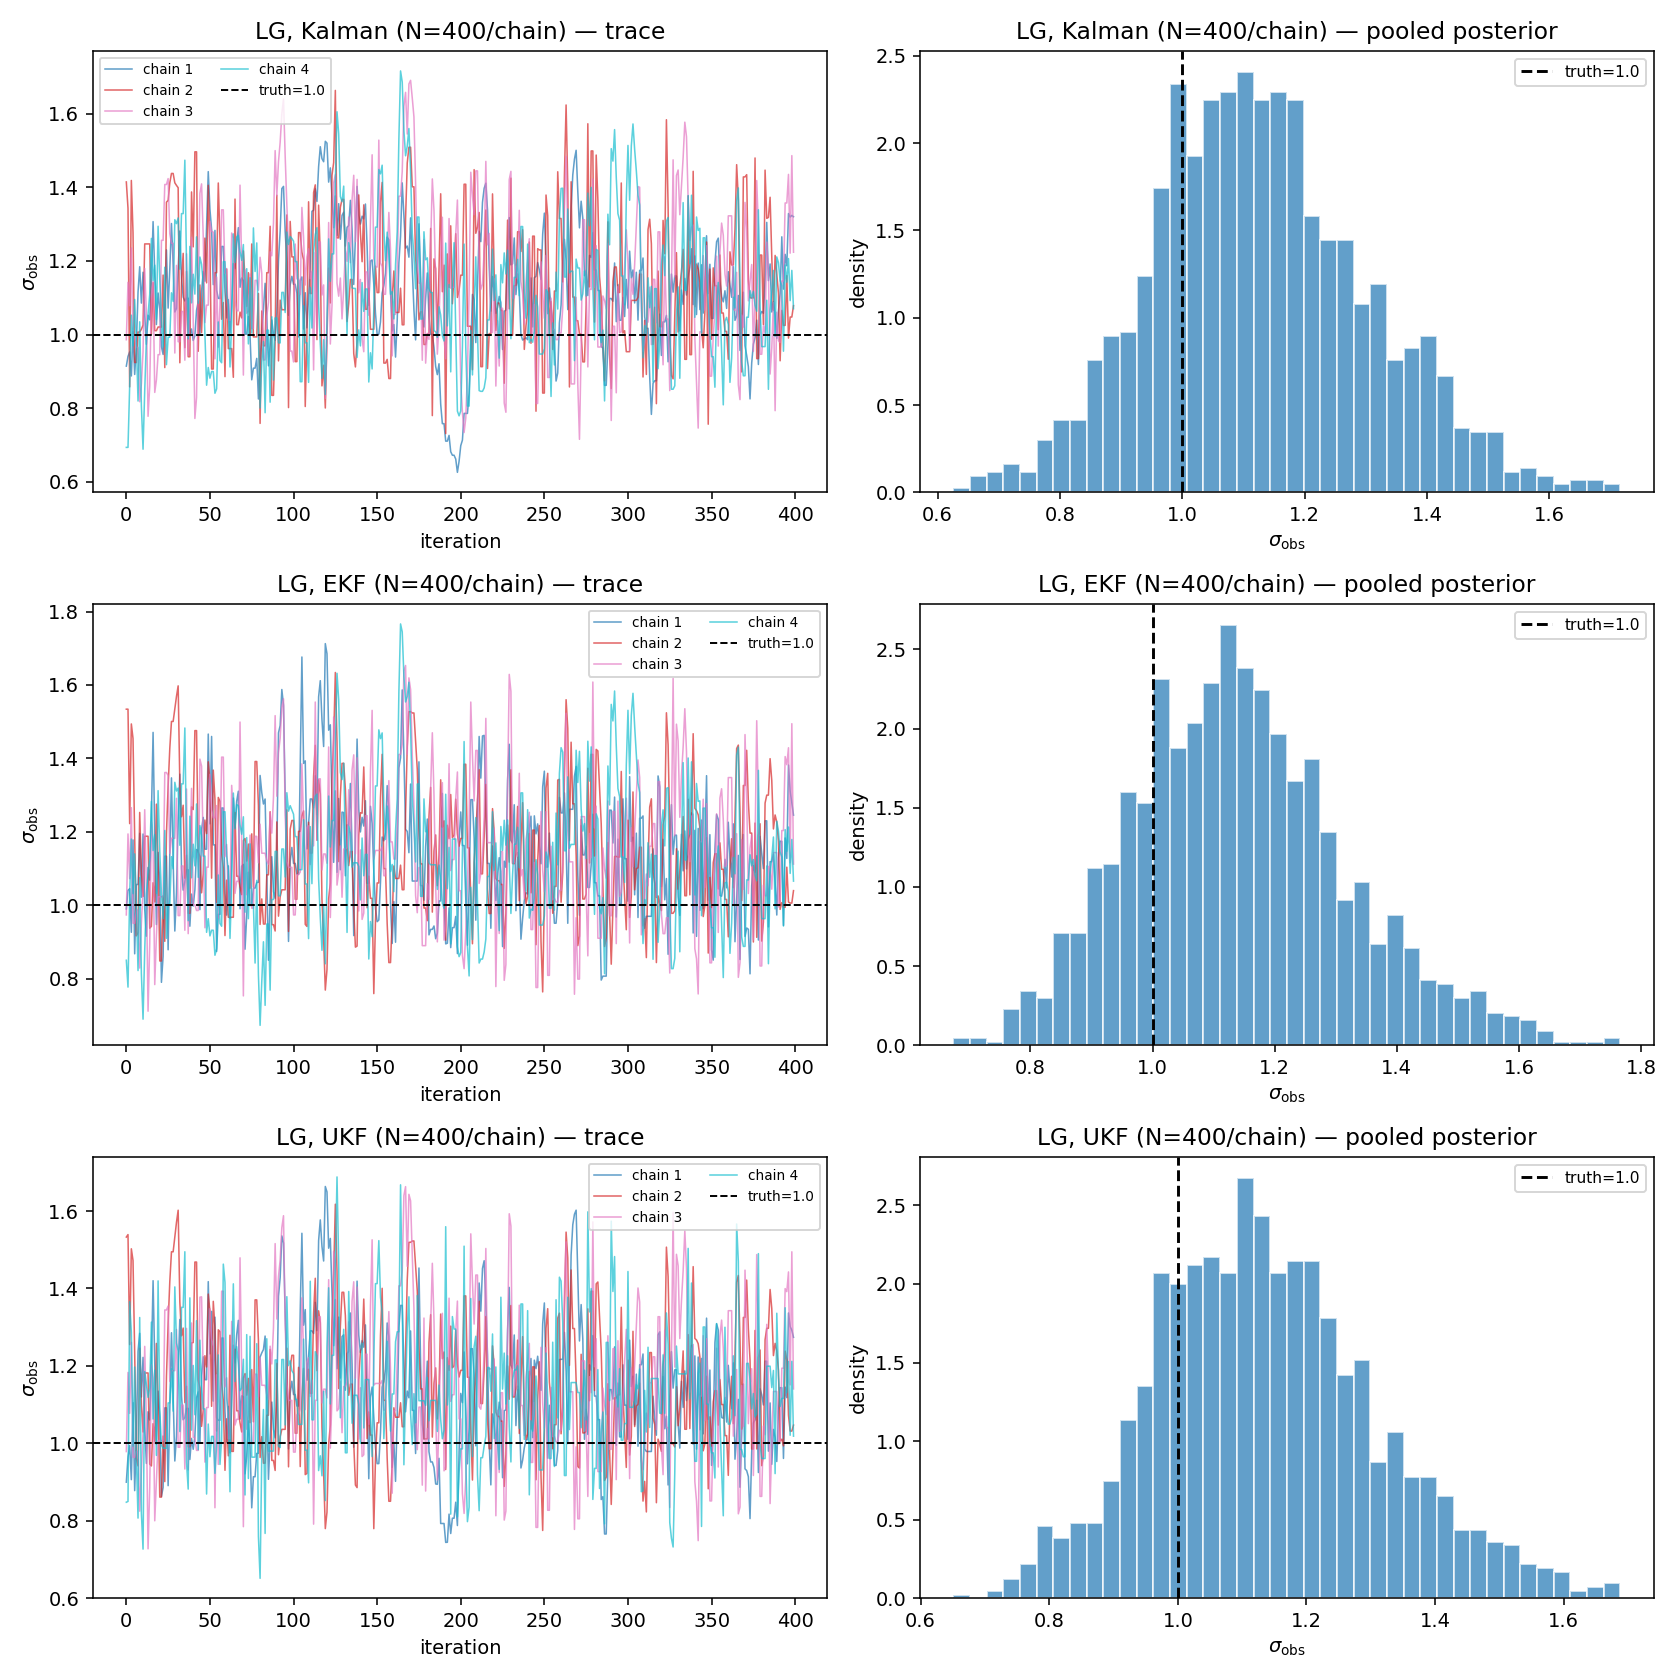
\includegraphics[width=0.95\linewidth]{figures/hmc_lg_kalman_family_4chain.png}
    \caption{1D LG four-chain HMC for the Kalman-family filters, post-burn-in. Rows: Kalman, EKF, UKF. Left column: traces, four chains overlaid in distinct colors with the truth $\sigma_{\text{obs}} = 1.0$ as the dashed horizontal line. Right column: pooled marginal posterior with truth at $1.0$ as the dashed vertical line. All three runs at \texttt{target\_accept\_prob} $= 0.65$, $400$ samples per chain.}
    \label{fig:hmc_lg_kalman_family_4chain}
\end{figure}

\subsubsection{1D Linear Gaussian (BPF+OT and LEDH+OT)}
\label{sec:hmc-multichain-lg}

Both differentiable filters target the same scalar parameter $\sigma_{\text{obs}}$ at true value $1.0$ on the same observation sequence as the Kalman family above. The chains initialize at $\sigma_{\text{obs}} \in \{0.5, 1.0, 1.5, 2.0\}$ for chains 1--4. BPF+OT requires an extended sample budget because the 400-sample run had split $\hat R = 1.087$; doubling the sample count to 2000 brings $\hat R$ down to $1.001$, with bulk ESS $7829$ and tail ESS $5638$ across all four chains. LEDH+OT converges at the original 400-sample budget with bulk ESS $672$ and tail ESS $634$. The per-chain final step sizes after dual-averaging are tightly clustered ($\varepsilon \approx 0.34$ for both filters, with chain-to-chain variation under $4\%$), confirming that DA settled consistently across independent inits.

Both filters deliver the same posterior centered near $1.20$, offset $+1.15\sigma$ from truth --- approximately $0.06$ above the Kalman-exact posterior mean reported above. The offset is realization-specific to this dataset; both differentiable filters infer the same posterior given the observation sequence, and the small upward shift relative to the analytic Kalman is consistent with the higher posterior variance the particle approximation exhibits at this $N = 500$ particle budget. This is a property of the data plus the filter's posterior width, not a chain failure. Table~\ref{tab:hmc_multichain_lg} (bottom two rows) gives the full diagnostics; Figure~\ref{fig:hmc_lg_4chain} shows the four-chain traces and the pooled posteriors.

\begin{table}[H]
\centering
\footnotesize
\caption{1D LG multi-chain diagnostics. Truth offset is $(\text{posterior mean} - \text{truth}) / \text{posterior sd}$; it measures realization-specific posterior centering and is not a chain-failure metric. ``Max $\hat R$'' is $\max(\text{bulk-}\hat R, \text{tail-}\hat R)$ on rank-normalized samples (Stan default); raw split-$\hat R$ on $\theta$ is also reported for comparison. All five filters target the same observation sequence and share the truth $\sigma_{\text{obs}} = 1.0$.}
\label{tab:hmc_multichain_lg}
\begin{tabular}{lccccccccc}
\toprule
Filter & Truth & Mean & Sd & 90\% CI & Offset/sd & Split $\hat R$ & Max $\hat R$ & Bulk ESS & Tail ESS \\
\midrule
Kalman        & $1.0$ & $1.127$ & $0.177$ & $[0.85, 1.44]$ & $+0.72$ & $1.004$ & $1.008$ & $278$  & $325$  \\
EKF           & $1.0$ & $1.142$ & $0.176$ & $[0.87, 1.46]$ & $+0.81$ & $1.002$ & $1.003$ & $419$  & $518$  \\
UKF           & $1.0$ & $1.138$ & $0.173$ & $[0.87, 1.45]$ & $+0.80$ & $1.002$ & $1.002$ & $464$  & $494$  \\
BPF+OT (long) & $1.0$ & $1.194$ & $0.168$ & $[0.92, 1.47]$ & $+1.15$ & $1.001$ & $1.001$ & $7829$ & $5638$ \\
LEDH+OT       & $1.0$ & $1.202$ & $0.179$ & $[0.91, 1.50]$ & $+1.13$ & $1.000$ & $1.002$ & $672$  & $634$  \\
\bottomrule
\end{tabular}
\end{table}

\begin{figure}[H]
    \centering
    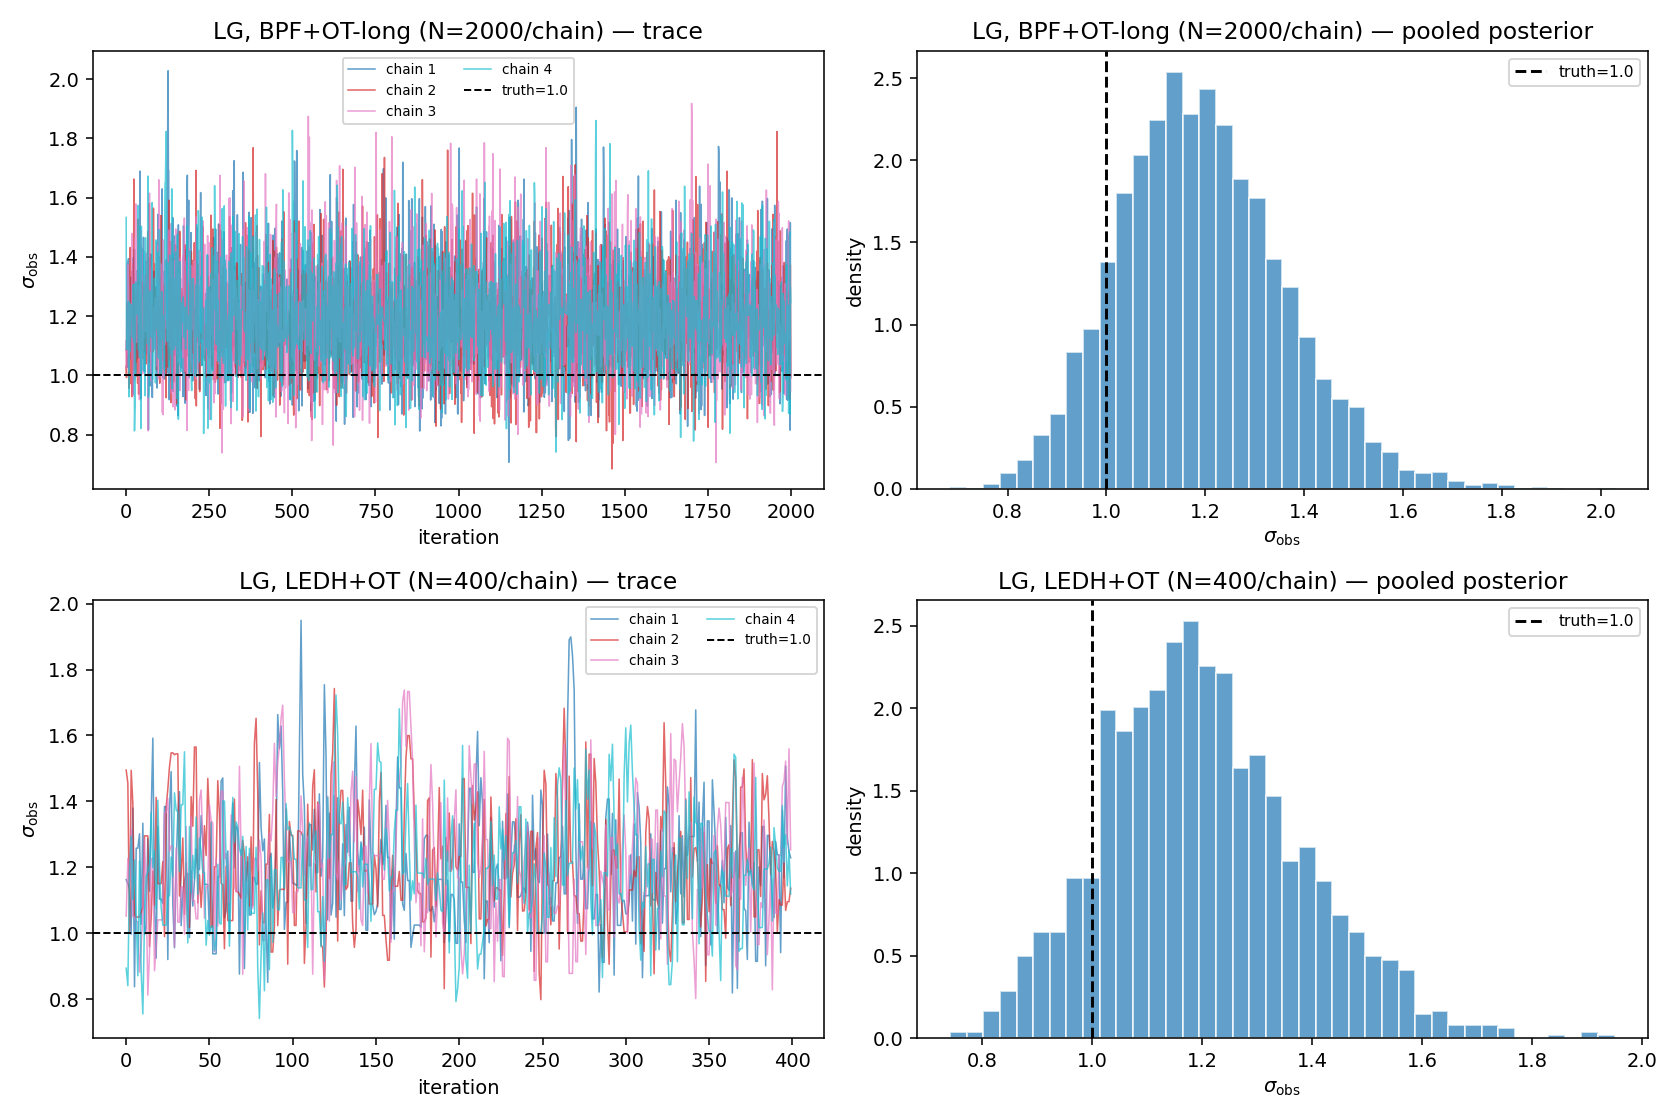
\includegraphics[width=0.95\linewidth]{figures/hmc_lg_4chain_combined.png}
    \caption{1D LG four-chain HMC, post-burn-in. Top row: BPF+OT with extended sample budget (2000 per chain). Bottom row: LEDH+OT (400 per chain). Left column: traces, four chains overlaid in distinct colors. Right column: pooled marginal posterior with truth at $1.0$ as the dashed vertical line.}
    \label{fig:hmc_lg_4chain}
\end{figure}

\subsubsection{1D Stochastic Volatility (LEDH+OT)}
\label{sec:hmc-multichain-sv1d}

The 1D SV chain estimates the persistence parameter $\alpha$ at true value $0.91$ on the log-squared-transformed model. Chains 1--4 initialize $\alpha \in \{0.6, 0.8, 0.91, 0.97\}$. The four-chain run converges with split $\hat R = 1.005$, bulk ESS $607$, and tail ESS $615$ over $400$ samples per chain. Final step sizes cluster at $\varepsilon \approx 0.40$ with acceptance $0.87$--$0.92$ across chains. The posterior mean is $0.921 \pm 0.028$, offset only $+0.38\sigma$ from truth --- the closest match in the converged Kalman-family-plus-flow runs above.

\begin{table}[H]
\centering
\footnotesize
\caption{1D SV multi-chain diagnostics, LEDH+OT. ``Max $\hat R$'' is $\max(\text{bulk-}\hat R, \text{tail-}\hat R)$ on rank-normalized samples.}
\label{tab:hmc_multichain_sv1d}
\begin{tabular}{ccccccccc}
\toprule
Truth & Mean & Sd & 90\% CI & Offset/sd & Split $\hat R$ & Max $\hat R$ & Bulk ESS & Tail ESS \\
\midrule
$0.91$ & $0.921$ & $0.028$ & $[0.876, 0.967]$ & $+0.38$ & $1.005$ & $1.005$ & $607$ & $615$ \\
\bottomrule
\end{tabular}
\end{table}

\begin{figure}[H]
    \centering
    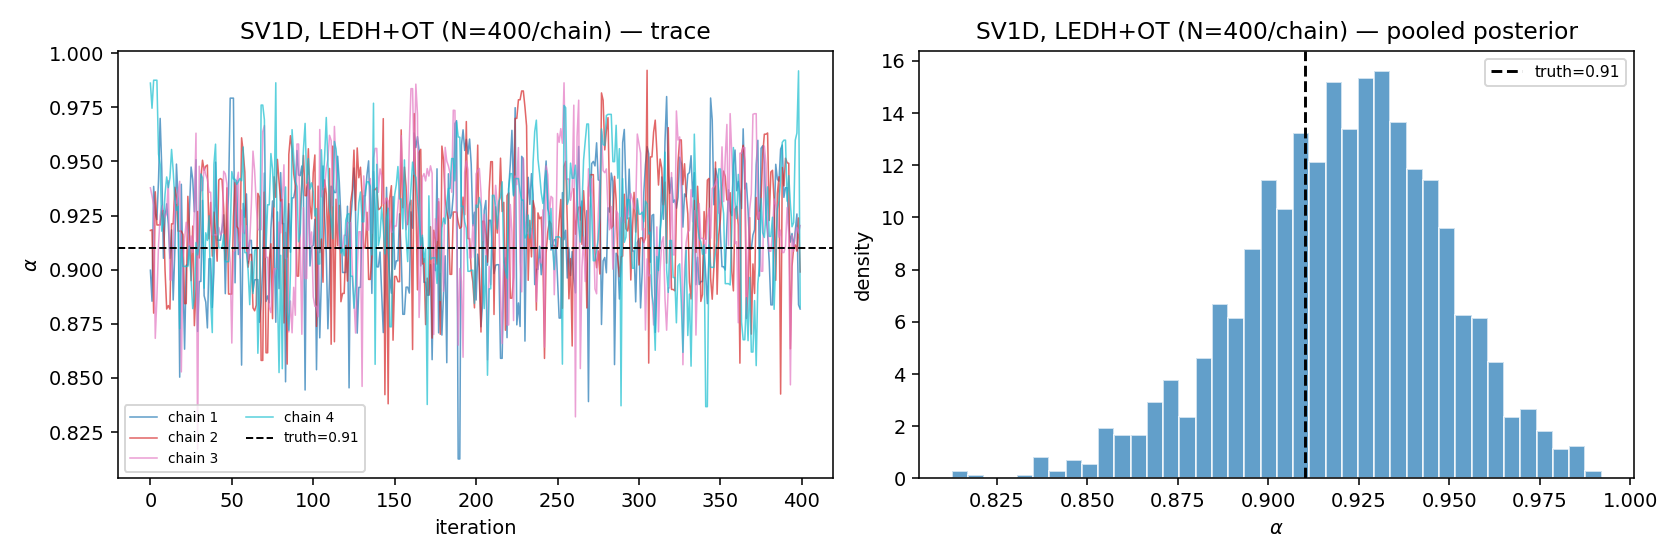
\includegraphics[width=0.95\linewidth]{figures/hmc_sv1d_4chain_combined.png}
    \caption{1D SV four-chain HMC, post-burn-in. Left: traces, four chains in distinct colors. Right: pooled marginal posterior for $\alpha$, dashed line at truth $0.91$.}
    \label{fig:hmc_sv1d_4chain}
\end{figure}

\subsubsection{Range-Bearing (LEDH+OT, Per-Axis Step + $L=10$)}
\label{sec:hmc-multichain-rb}

Range-bearing is the case that exposed the most multi-chain tuning effort. The default scalar-step LEDH+OT config gives split $\hat R = 1.003$ on $\sigma_{\text{range}}$ but $1.094$ on $\sigma_{\text{bearing}}$. Per-chain bearing standard deviations vary by a factor of $1.83$ across the four chains while the bearing means agree --- the chains converge to the same posterior centering but disagree on the posterior width. That signature points to per-axis mixing rate: $\sigma_{\text{bearing}}$ has both a narrower posterior in unconstrained space (q-space std $0.110$ versus $0.146$ for $\sigma_{\text{range}}$) and a noisier likelihood gradient via the $\arctan2$ observation, so the bearing axis explores its tails more slowly than range under a shared scalar step.

%A diagonal mass-matrix attempt $M = \mathrm{diag}(1/\mathrm{Var}(q)) = [47.26,\,82.09]$ crashed during burn-in. The larger random-momentum scale ($|p| \sim \sqrt{M} \approx 7\text{--}9$ per axis) dominated the gradient signal in the first iterations, producing $100\%$ acceptance trivially, which DA misread as ``step too small''. DA then grew the step exponentially until the OT backward MatrixSolve became singular and the chain crashed at burn-in step 19. Stan-style windowed mass-matrix adaptation re-initializes the step size after each metric update; the single-pass offline approach used here does not, and that mismatch is what failed.

The successful configuration introduce per-axis step sizes $\varepsilon = [\,0.001,\,0.004\,]$ --- range axis at the original scalar value, bearing axis four times larger. DA preserves the $4\times$ ratio because its scalar log-step update applies identically to both axes.  Adding $L = 10$ leapfrog steps per HMC iteration (versus the default $L = 5$) doubles the trajectory length per iteration and cuts $\sigma_{\text{bearing}}$ split $\hat R$ further, from $1.025$ at $L = 5$ to $1.005$ at $L = 10$. Final adapted step sizes across chains are $\varepsilon \approx [\,0.034,\,0.137\,]$ with the $4\times$ ratio preserved. Acceptance is $0.86$--$0.91$ across chains.

The posterior mean for $\sigma_{\text{range}}$ is $0.107 \pm 0.014$ ($+0.49\sigma$ from truth), and for $\sigma_{\text{bearing}}$ is $0.130 \pm 0.016$ ($+1.86\sigma$ from truth). The bearing offset is realization-specific: a separate 1D likelihood scan at $\sigma_{\text{range}}$ fixed to truth shows $\sigma_{\text{bearing}}$'s empirical likelihood peaks near $0.119$ regardless of particle count, $\lambda$-step count, or seed, indicating the offset is a property of this $T = 50$ observation sequence rather than a chain failure.

\begin{table}[H]
\centering
\footnotesize
\caption{Range-bearing multi-chain diagnostics, LEDH+OT with axisstep and $L=10$. ``Max $\hat R$'' is $\max(\text{bulk-}\hat R, \text{tail-}\hat R)$ on rank-normalized samples.}
\label{tab:hmc_multichain_rb}
\begin{tabular}{lccccccccc}
\toprule
Parameter & Truth & Mean & Sd & 90\% CI & Offset/sd & Split $\hat R$ & Max $\hat R$ & Bulk ESS & Tail ESS \\
\midrule
$\sigma_{\text{range}}$  & $0.10$ & $0.107$ & $0.014$ & $[0.084, 0.130]$ & $+0.49$ & $0.998$ & $1.000$ & $1600$ & $1092$ \\
$\sigma_{\text{bearing}}$ & $0.10$ & $0.130$ & $0.016$ & $[0.106, 0.154]$ & $+1.86$ & $1.005$ & $1.007$ & $632$  & $787$  \\
\bottomrule
\end{tabular}
\end{table}

\begin{figure}[H]
    \centering
    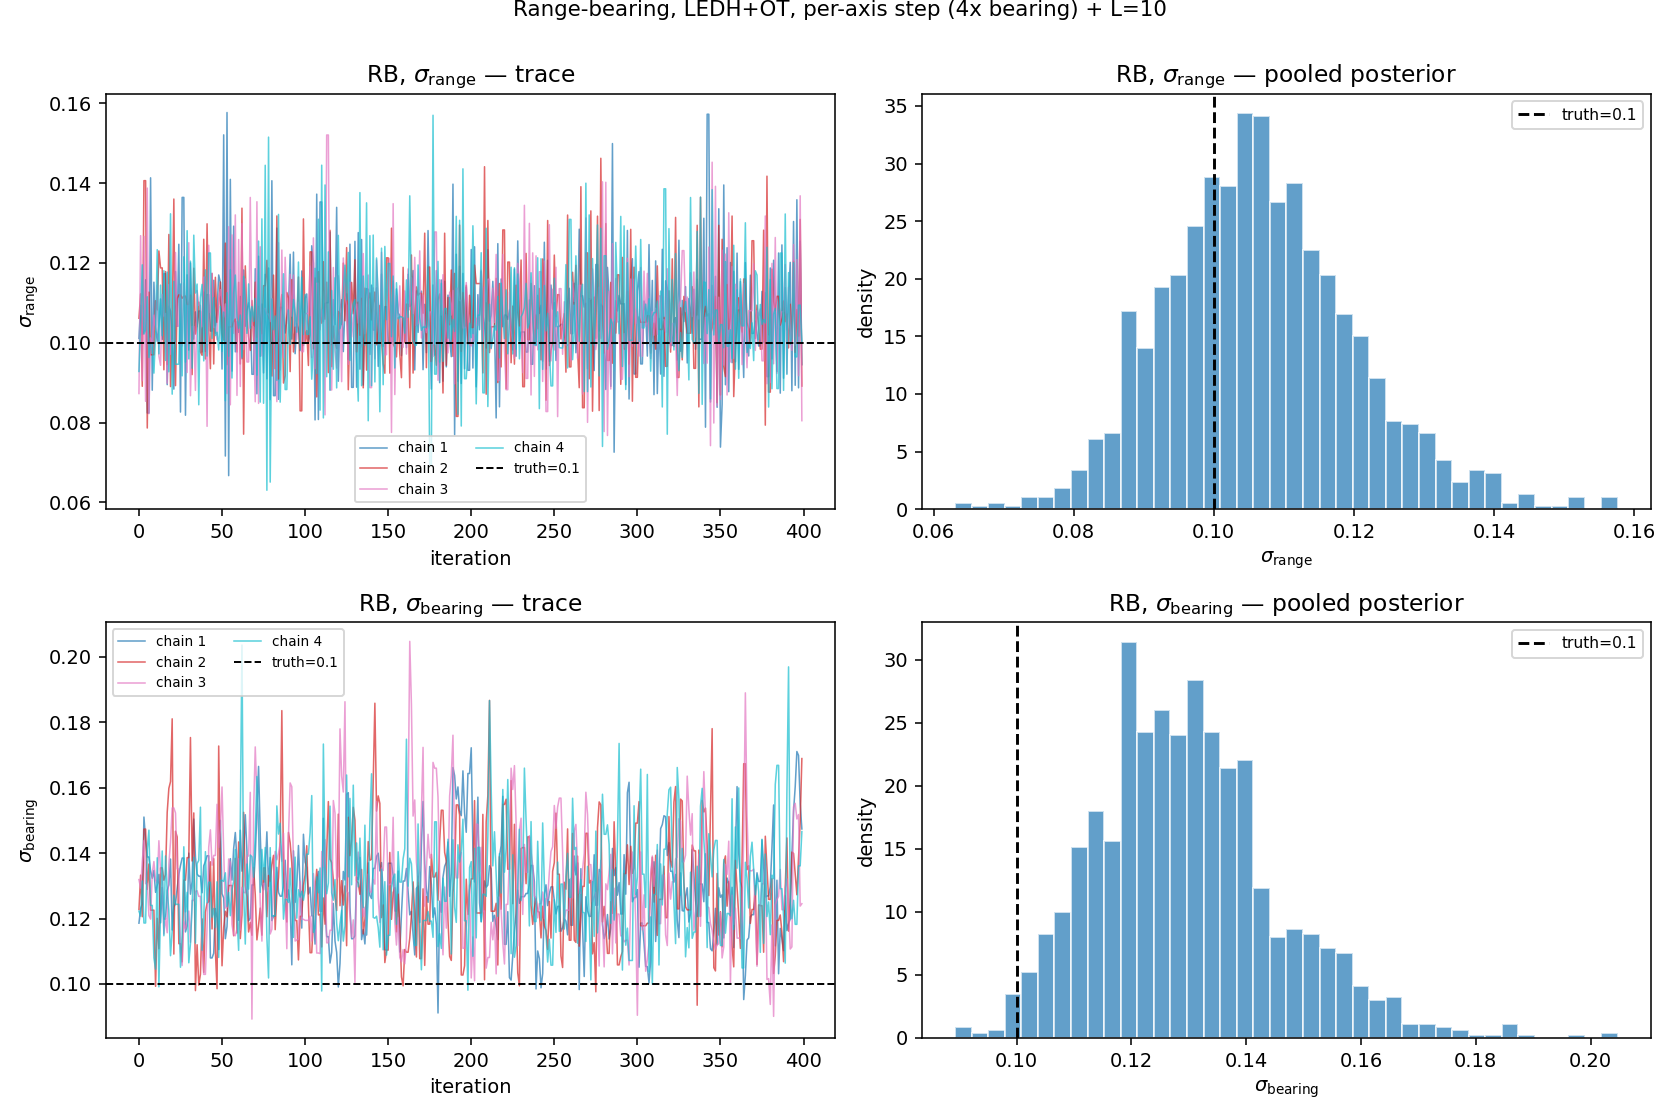
\includegraphics[width=0.95\linewidth]{figures/hmc_rb_4chain_combined.png}
    \caption{Range-bearing four-chain HMC, post-burn-in. Top row: $\sigma_{\text{range}}$. Bottom row: $\sigma_{\text{bearing}}$. Left column: four-chain traces. Right column: pooled marginal posteriors with dashed lines at the true values ($0.10$ for both).}
    \label{fig:hmc_rb_4chain}
\end{figure}

\paragraph{Cross-comparison.}
Across the four converged runs, split $\hat R$ ranges from $0.998$ to $1.005$, all well below the $1.01$ Vehtari threshold. Bulk ESS varies by an order of magnitude, driven mostly by sample budget: BPF+OT-long has $7829$ at $N=2000$ per chain, the four-hundred-sample runs sit at $607\text{--}1600$. Tail ESS tracks bulk closely, indicating no severe tail-sampling deficiency. The truth offset, by contrast, is dataset-specific and unrelated to chain quality: the closest hit is SV1D at $+0.38\sigma$, the largest is range-bearing's bearing parameter at $+1.86\sigma$. The offset says how informative this particular observation sequence is about the parameter, not whether the chain found that information.

The cost differs sharply across runs. BPF+OT-long is the cheapest per sample (acceptance $0.77$, scalar step) but needed $5\times$ more samples. Range-bearing was the most expensive per sample (twice the leapfrog budget, two-axis step tuning) and needed the most engineering to converge. SV2D remains the open case --- the OT backward instability under the gradient path that worked for the other models is the open failure case noted in the Limitations subsection.

% --- SV2D gradient-diagnostics subsection commented out; the failure case is
% --- summarised inline in the cross-comparison paragraph and the Limitations
% --- subsection. Source preserved.
\iffalse
\subsection{Gradient Diagnostics on SV2D: Unresolved Nonlinear Failure}
\label{sec:sv2d}

The linear Gaussian benchmark validates the HMC machinery. This subsection documents where it breaks: HMC on the 2D stochastic volatility model (SV2D) with either a bootstrap particle filter or the LEDH flow filter, both combined with OT resampling. The failure is not in the filter itself --- §4 shows LEDH tracks SV2D with reasonable RMSE --- it is in the gradient path that feeds HMC.
The SV2D runs use the same Lyapunov-stationary construction for the stable diagonal transition matrix as the 1D SV case in \S\ref{par:init-conditions}; the initial-state prior is therefore not a candidate root cause for the failure mode described below.

Figures~\ref{fig:hmc_sv2d_trace} and~\ref{fig:hmc_sv2d_histogram} show the post-burn-in chain. The aggregate diagnostics for this single-chain SV2D run are: acceptance $0.75$, ESS $27.9$, split-$\hat R$ $1.021$, $500$ samples / $200$ burn-in, $L = 5$ leapfrog steps, wall time $36{,}456$ seconds.

\begin{figure}[H]
    \centering
    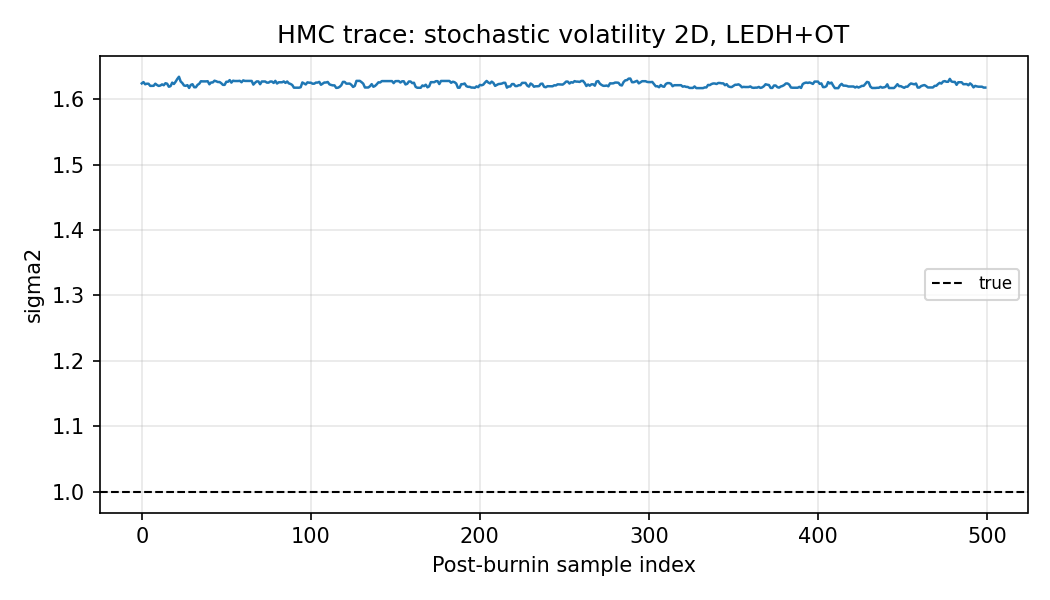
\includegraphics[width=0.7\linewidth]{hmc_sv2d_trace.png}
    \caption{2D stochastic volatility HMC post-burn-in trace for $\sigma_2$, LEDH+OT filter. Dashed reference line at the true value $1.0$. The trace oscillates around the truth but see the paragraphs below for why this is insufficient to call the run a success.}
    \label{fig:hmc_sv2d_trace}
\end{figure}

\begin{figure}[H]
    \centering
    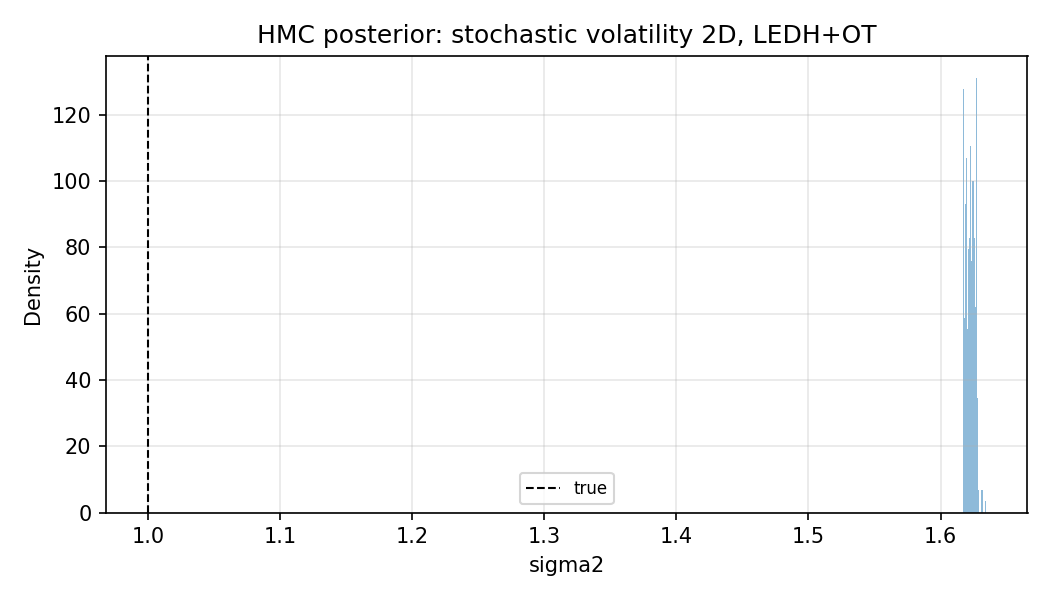
\includegraphics[width=0.7\linewidth]{hmc_sv2d_histogram.png}
    \caption{2D stochastic volatility HMC marginal posterior for $\sigma_2$, LEDH+OT filter. The posterior is broader than the SV1D and LG cases, reflecting the step-level gradient instability discussed below.}
    \label{fig:hmc_sv2d_histogram}
\end{figure}

\paragraph{Symptom.} During leapfrog integration, the gradient $\nabla_{\boldsymbol{\theta}} U$ occasionally spikes by several orders of magnitude, $\Delta H$ blows up, and individual proposals can be rejected. In the run shown above, the aggregate acceptance rate is $0.75$ and split-$\hat R$ is $1.02$, so the usual chain-level diagnostics look acceptable. The problem is more local: ESS is only $27.9$ over $500$ samples, and the spikes appear at specific leapfrog substeps rather than uniformly across the trajectory. An aggregate-only diagnostic would miss this failure.

\paragraph{What I have ruled out.} A fixed-seed vs.\ fresh-seed MAP comparison shows that the instability persists even when the particle seed is held constant, so the spikes are not just estimator variance from the stochastic particle filter averaging out over many steps. A loss-surface scan across a 2D slice of parameter space exhibits sharp discontinuities that are absent on the 1D linear Gaussian surface; this indicates the problem is in the loss surface itself, not in integrator tuning.

\paragraph{Working hypotheses.} Table~\ref{tab:sv2d-hypotheses} lists the current candidates for the root cause, the evidence for and against each, and the test that would rule them in or out.

\begin{table}[H]
\centering
\footnotesize
\caption{Candidate root causes for the SV2D HMC gradient failure.}
\label{tab:sv2d-hypotheses}
\begin{tabular}{p{3.4cm}p{3.8cm}p{3.8cm}p{2.2cm}}
\toprule
Hypothesis & Evidence for & Evidence against & Status \\
\midrule
ESS-threshold branch discontinuity in conditional resampling & Spikes coincide with timesteps where ESS crosses the resample threshold; 1D Gaussian (no such crossings in typical runs) is clean. & Same spike pattern reported on runs with unconditional resampling in small tests. & Open \\
SV2D integration of the implicit Sinkhorn backward & Theoretical: §\ref{sec:sinkhorn-backward} shows the extrapolation is known to be biased for Term 1, and SV2D activates that term strongly. & The remaining gap is the full SV2D HMC inner loop; see the closing framing below. & Open \\
LEDH flow-gradient (particle geometry term) bias & Appears on LEDH+OT; same spike geometry on BPF+OT suggests the flow is not the sole cause. & Cross-filter persistence argues against LEDH being the single culprit. & Partially ruled out \\
Stochastic PF estimator variance & Would average out with fresh seeds. & Fixed-seed runs still spike; fresh-seed runs still spike. & Ruled out \\
Initial-state prior choice & none & Lyapunov-stationary, matches §2 principle and the 1D SV case which converges cleanly & Ruled out \\
\bottomrule
\end{tabular}
\end{table}

\paragraph{Closing framing.}
\emph{The linear Gaussian multi-chain benchmark in \S\ref{sec:hmc-multichain-lg} validates the HMC machinery: MAP converges, gradients match finite differences, HMC posteriors match the Kalman reference. On SV2D, gradient spikes during leapfrog integration make the chain explore poorly even when aggregate acceptance looks acceptable. I have localised the failure to the nonlinear filter gradient path but have not isolated the root cause. The implicit Sinkhorn backward is derived and validated at the filter-gradient level in \S\ref{sec:ot-derivative-chain}; what I have not done is run the SV2D HMC inner loop with that backward and a branch-free conditional-resampling path. This limits the nonlinear DPF-HMC claims but does not affect the filtering results in \S\ref{sec:particle-methods-section} or the validation of the linear pipeline.}
\fi

\subsection{Limitations}

To collect the caveats that have been raised section-by-section: the differentiable-filter HMC pipeline is validated cleanly on linear Gaussian targets and on 1D SV and range-bearing under retuned multi-chain settings (\S\ref{sec:hmc-multichain}); SV2D is the remaining open case --- the single-chain run shows step-level gradient spikes that don't fold into aggregate acceptance ($0.75$) and the multi-chain attempt crashed in the OT backward pass with a singular MatrixSolve, which I did not isolate further in this report.
% 
% % \newpage
% 
% 
% % \section{A few words of reflection}
% % This is a well-structured test and I learned a lot from doing the background research, especially the knowledge I gained about Optimal Transport, which might actually turn out to be useful in the future. I now intend to learn about other applications of filtering and experiment with them more.
% 
% % I didn’t completely finish the test. I only included the experiments that directly relate to the question, even though I ran quite a few others. I simply ran out of time to write up the results properly.
% % I appreciate the experience. It made me realize that I need to manage my time better when navigating multiple commitments. I put too much focus on reading background material and exploring ideas for using neural networks to improve filtering. In the end, I didn’t have enough time left to debug the code, complete the experiments, or write tests that would actually catch numerical instability. During my academic years, I never had to write formal tests for my code, so this was by far the biggest challenge I’ve faced. My original plan was to first make things work, then go back and add tests to check the edge cases. Maybe that approach just doesn’t work well when I’m adding tests after the fact.
% % I will continue working on this project and force myself to write proper tests to debug the invertible flow code. Right now I still cannot reproduce the results from \cite{Li-Particle-Filtering-2017}, because the acoustic tracking model breaks all of my EDH flow, EDH invertible, and their local counterparts.
% 
% % Thank you for giving me this opportunity to do the test!
% 
% 
% % \newpage
% % \appendix
% 
% 
% \subsection{Benchmarking: From 1D Linear to Complex Models}
% 
% \subsubsection{Benchmarking HMC}
% For this part, we use Kalman family to test the HMC convergence. If it works here, this is useful baseline for particle filter. We used 100 burn-in steps and 200 sample, with 0.9 target acceptance rate. The blue histogram is the sample distribution and the dark vertical line is the true value corresponding to the data.
% 
% % \begin{figure}[H]
% %     \centering
% %     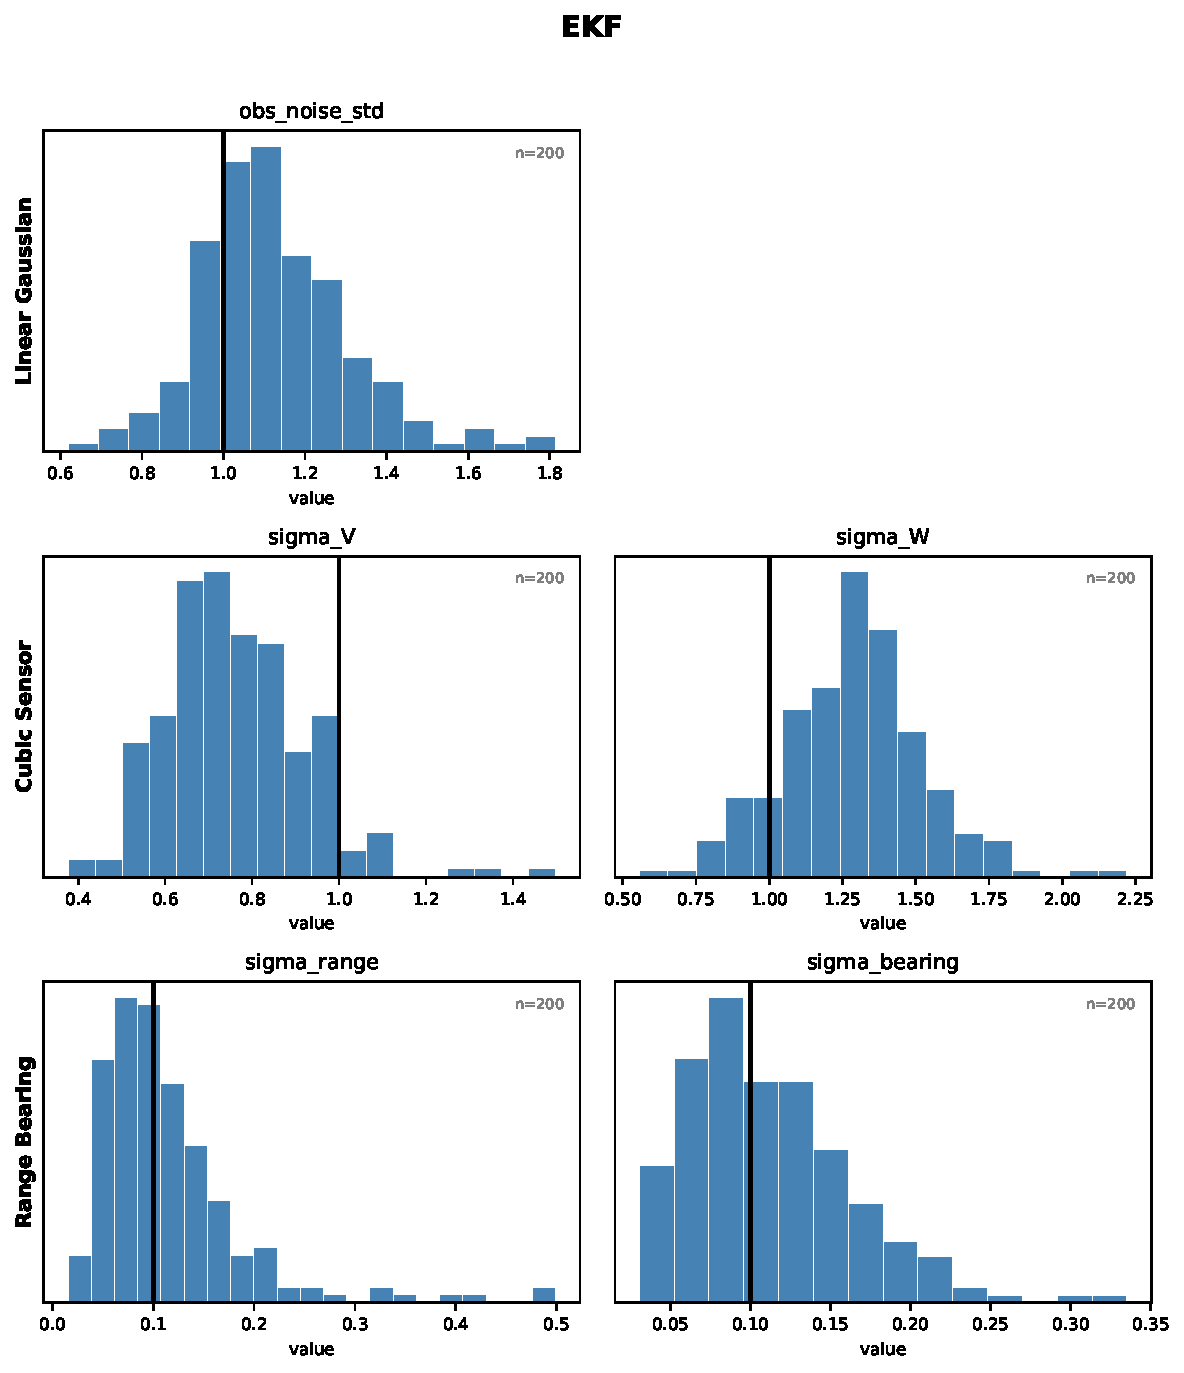
\includegraphics[width=0.45\textwidth]{hmc_ekf.pdf}
% %     \caption{EKF-based HMC posteriors across three models: Linear Gaussian, Cubic Sensor, and Range Bearing. Black lines indicate true parameter values.}
% %     \label{fig:hmc_ekf}
% % \end{figure}
% 
% % \begin{figure}[H]
% %     \centering
% %     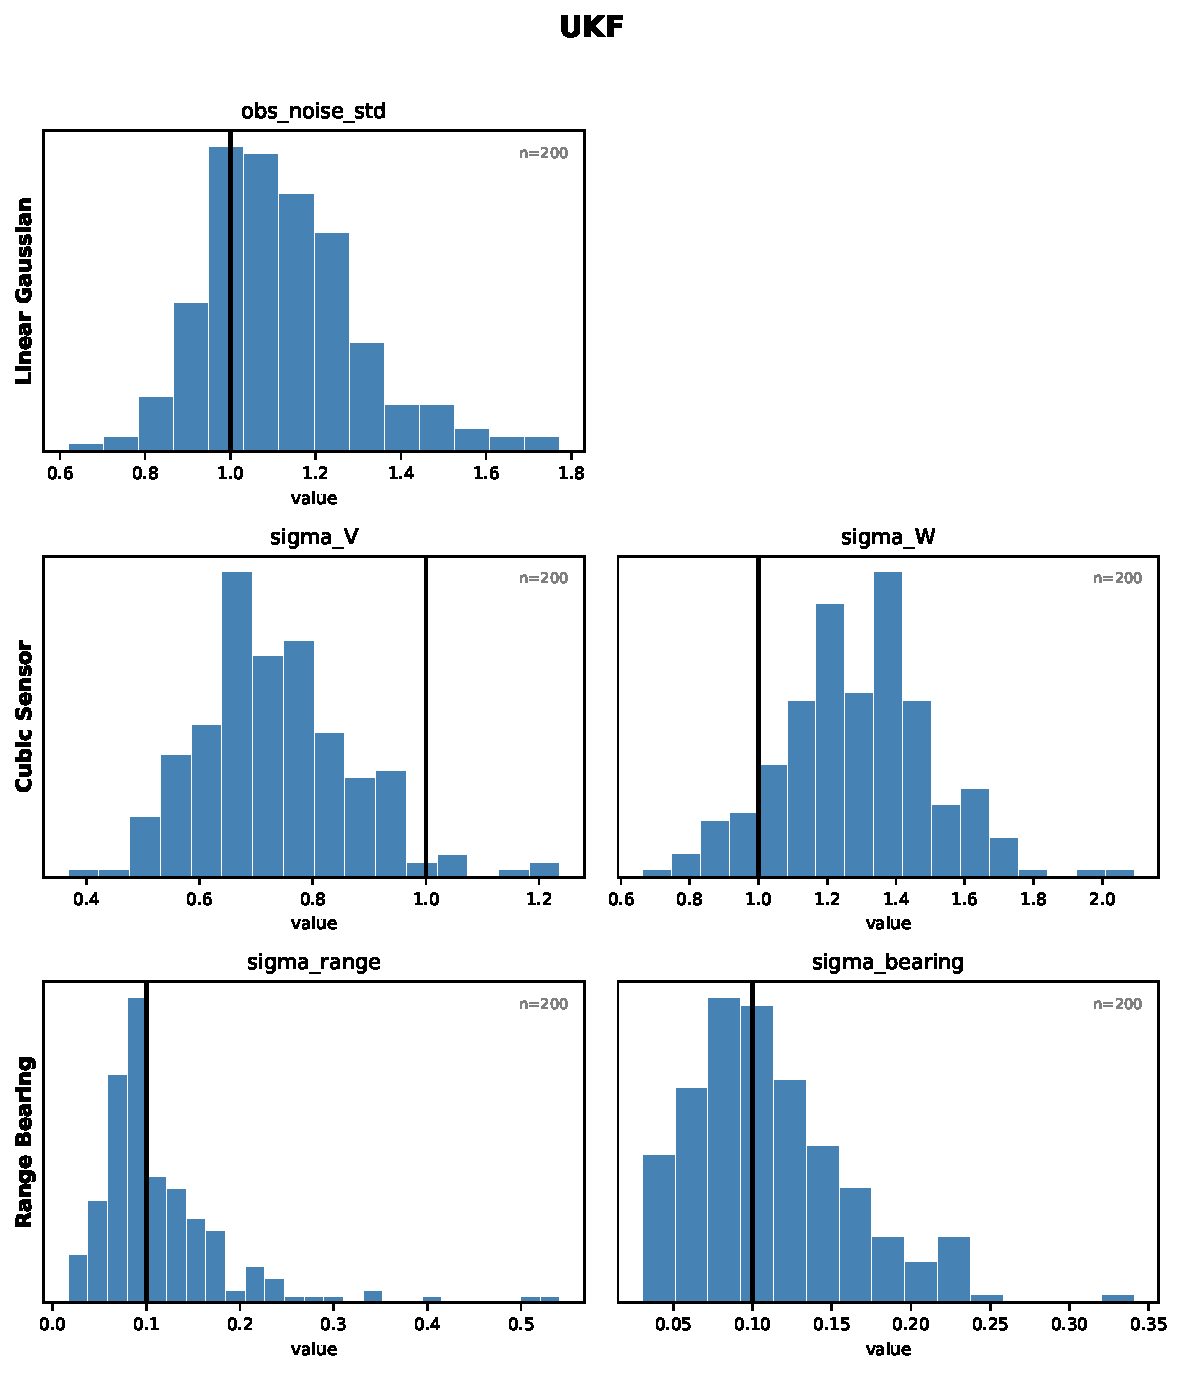
\includegraphics[width=0.45\textwidth]{hmc_ukf.pdf}
% %     \caption{UKF-based HMC posteriors across three models: Linear Gaussian, Cubic Sensor, and Range Bearing. Black lines indicate true parameter values.}
% %     \label{fig:hmc_ukf}
% % \end{figure}
% 
% Observation: The pipeline worked well for 1-d Gaussian linear and 2-d range bearing model. As for cubic sensor, we need careful tuning to make it better. However the pipeline is still stable. 
% 
% \subsubsection{Benchmarking particle filter and different resampling methods}
% A key observation is that, if the kalman family works for a model, then differentiable resampling + particle filter combo is not appropriate architecture for Bayesian inference.
% 
% % \begin{figure}[H]
% %     \centering
% %     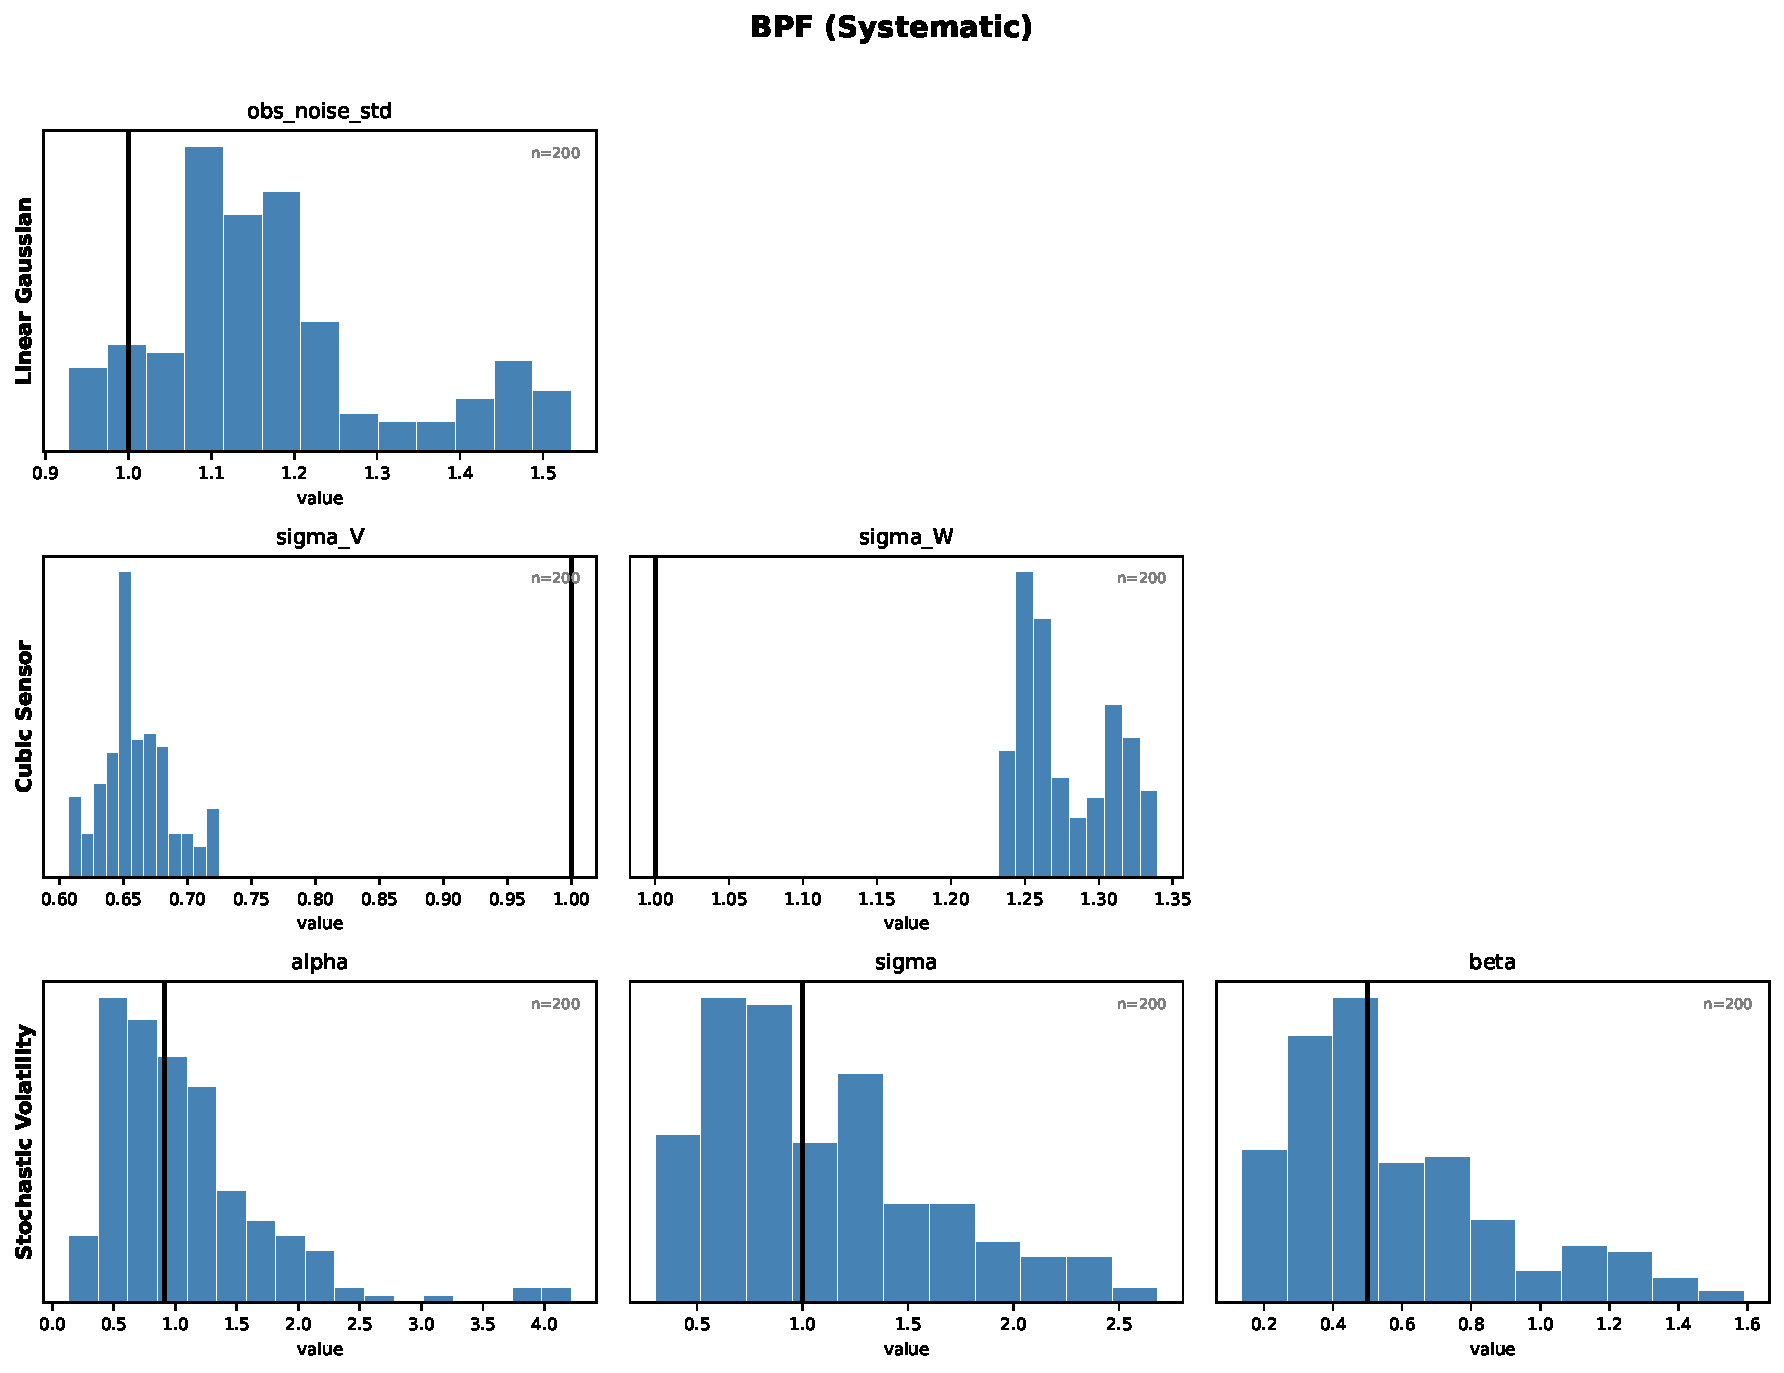
\includegraphics[width=0.8\textwidth]{hmc_bpf_sys.pdf}
% %     \caption{BPF with systematic resampling: HMC posteriors across Linear Gaussian, Cubic Sensor, and Stochastic Volatility. }
% %     \label{fig:hmc_bpf_sys}
% % \end{figure}
% 
% % \begin{figure}[H]
% %     \centering
% %     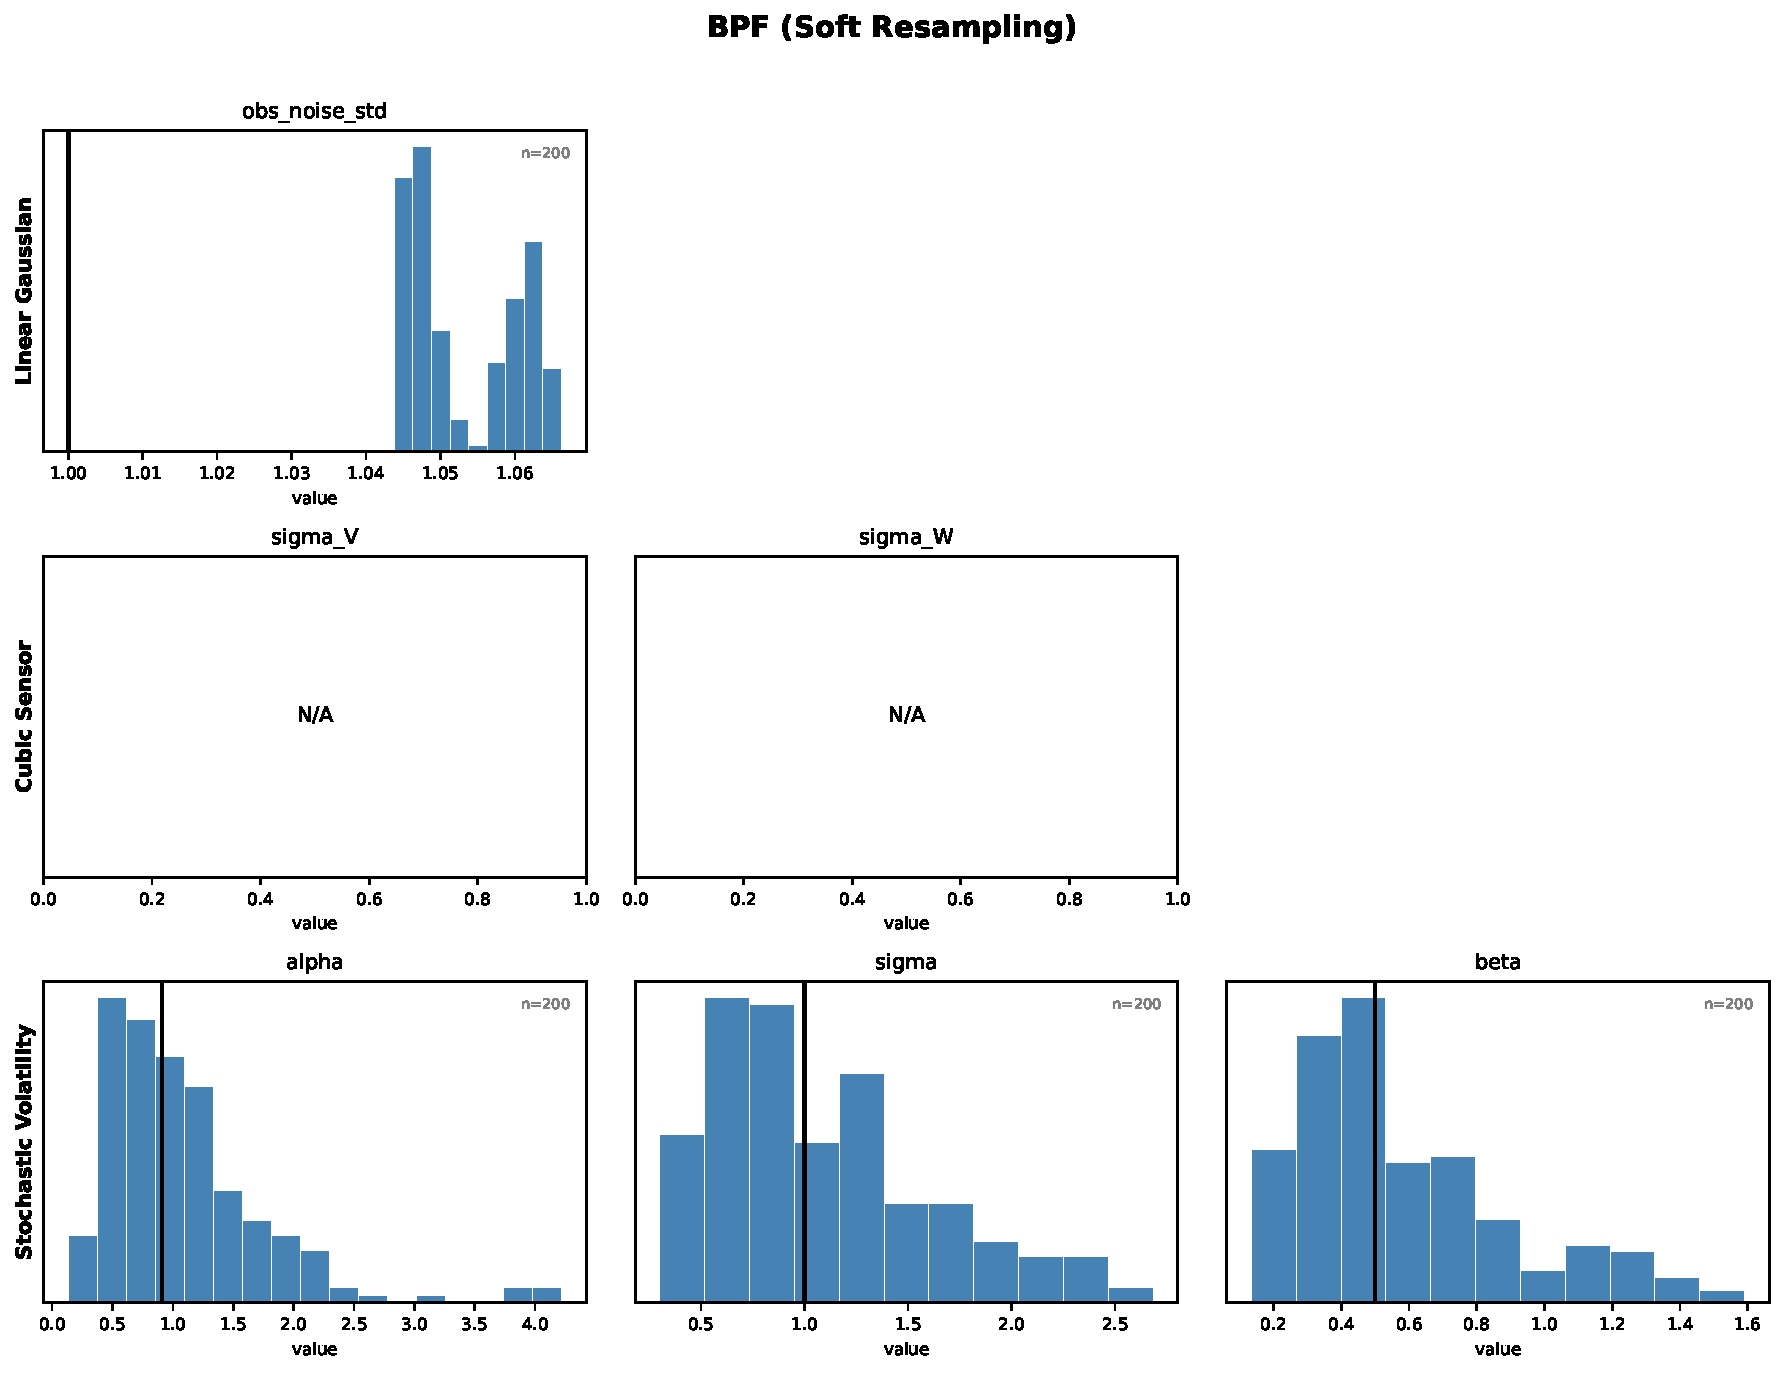
\includegraphics[width=0.8\textwidth]{hmc_bpf_soft.pdf}
% %     \caption{BPF with soft resampling: HMC posteriors across Linear Gaussian, Cubic Sensor, and Stochastic Volatility. }
% %     \label{fig:hmc_bpf_soft}
% % \end{figure}
% 
% % \begin{figure}[H]
% %     \centering
% %     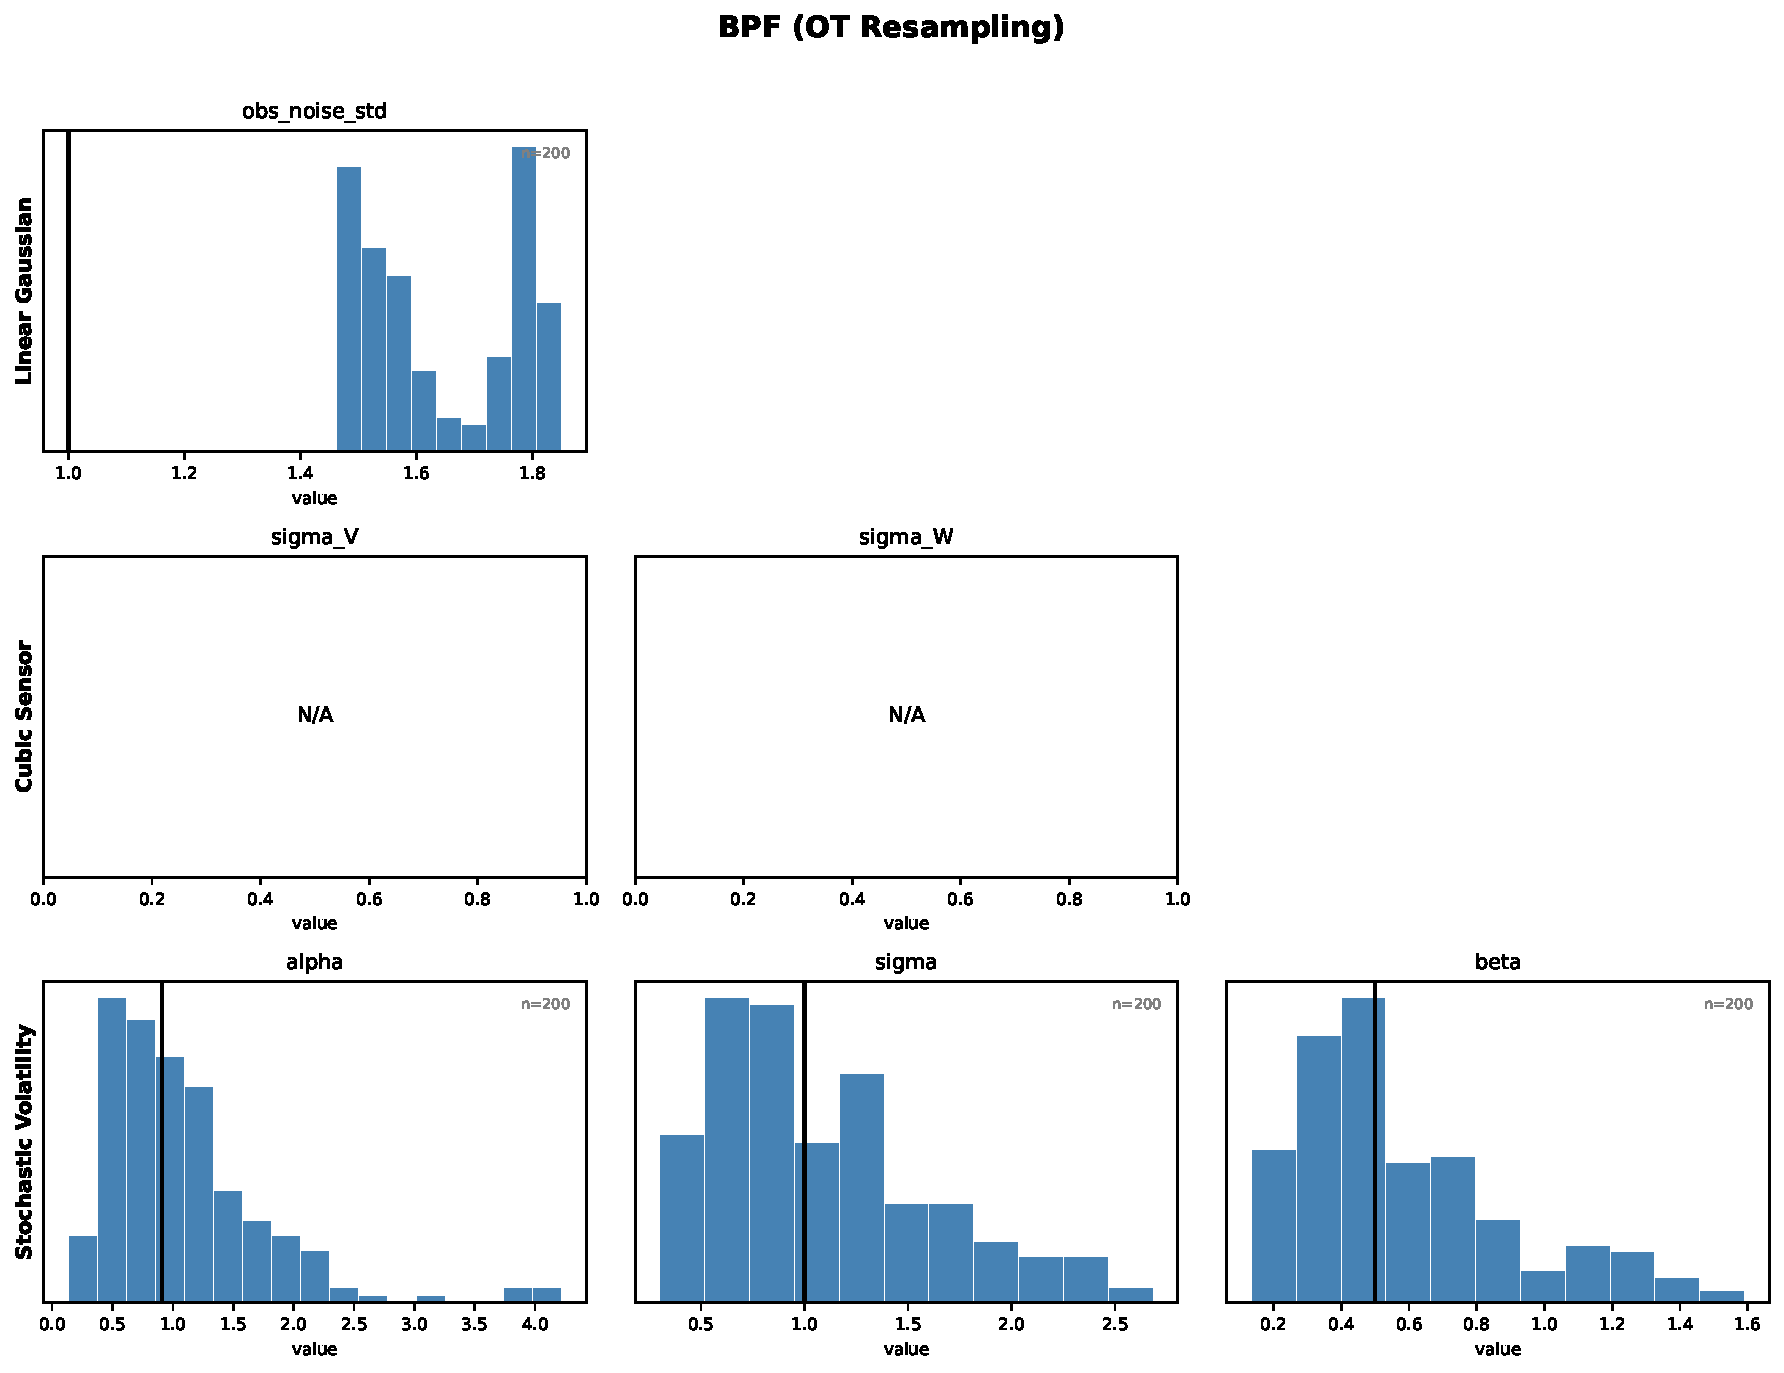
\includegraphics[width=0.8\textwidth]{hmc_bpf_ot.pdf}
% %     \caption{BPF with OT resampling: HMC posteriors across Linear Gaussian, Cubic Sensor, and Stochastic Volatility. }
% %     \label{fig:hmc_bpf_ot}
% % \end{figure}
% 
% % \begin{figure}[H]
% %     \centering
% %     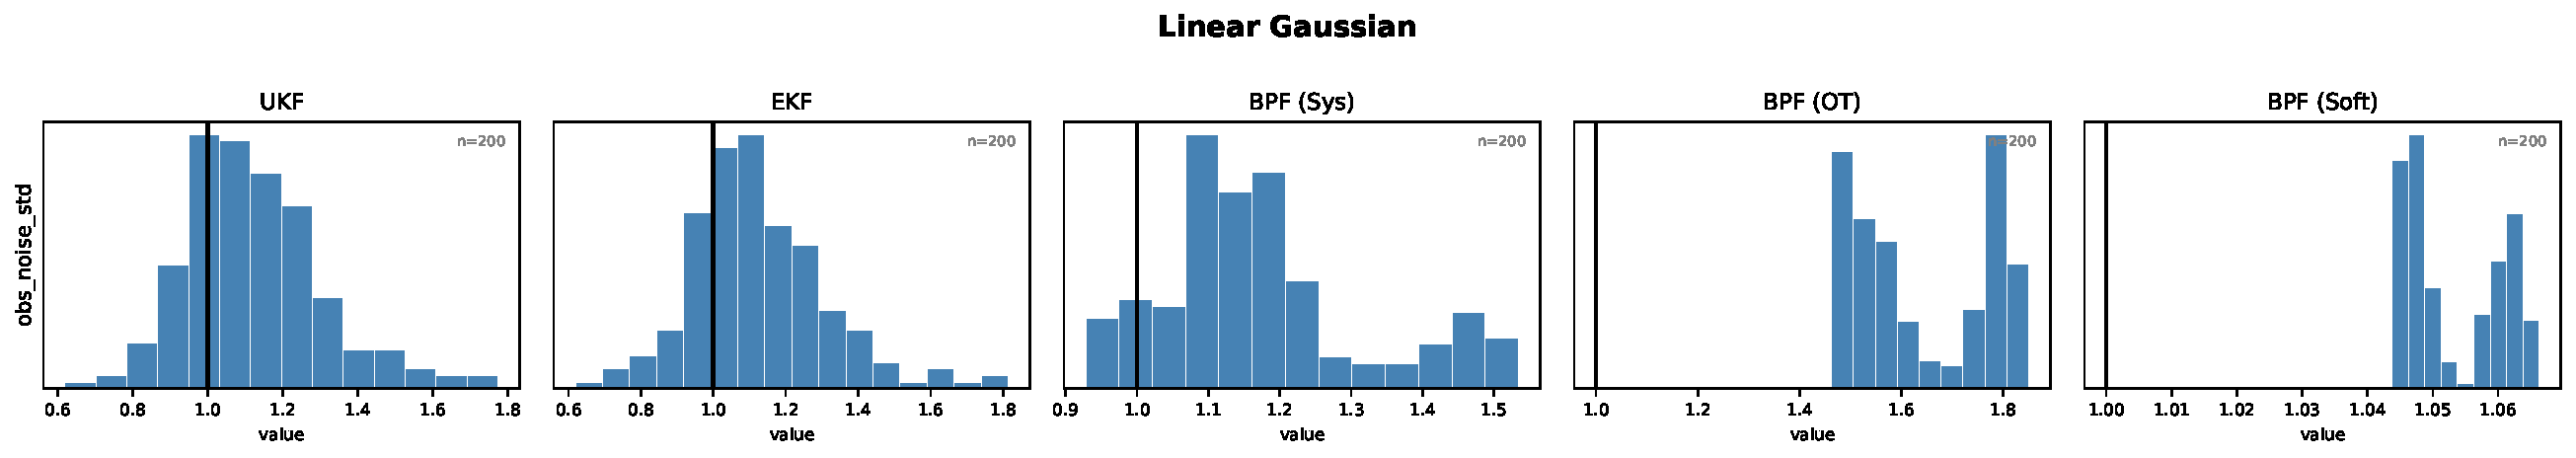
\includegraphics[width=\textwidth]{hmc_linear_gaussian.pdf}
% %     \caption{Linear Gaussian: HMC posteriors across all methods (UKF, EKF, BPF with systematic, OT, and soft resampling). }
% %     \label{fig:hmc_linear_gaussian}
% % \end{figure}
% 
% % \begin{figure}[H]
% %     \centering
% %     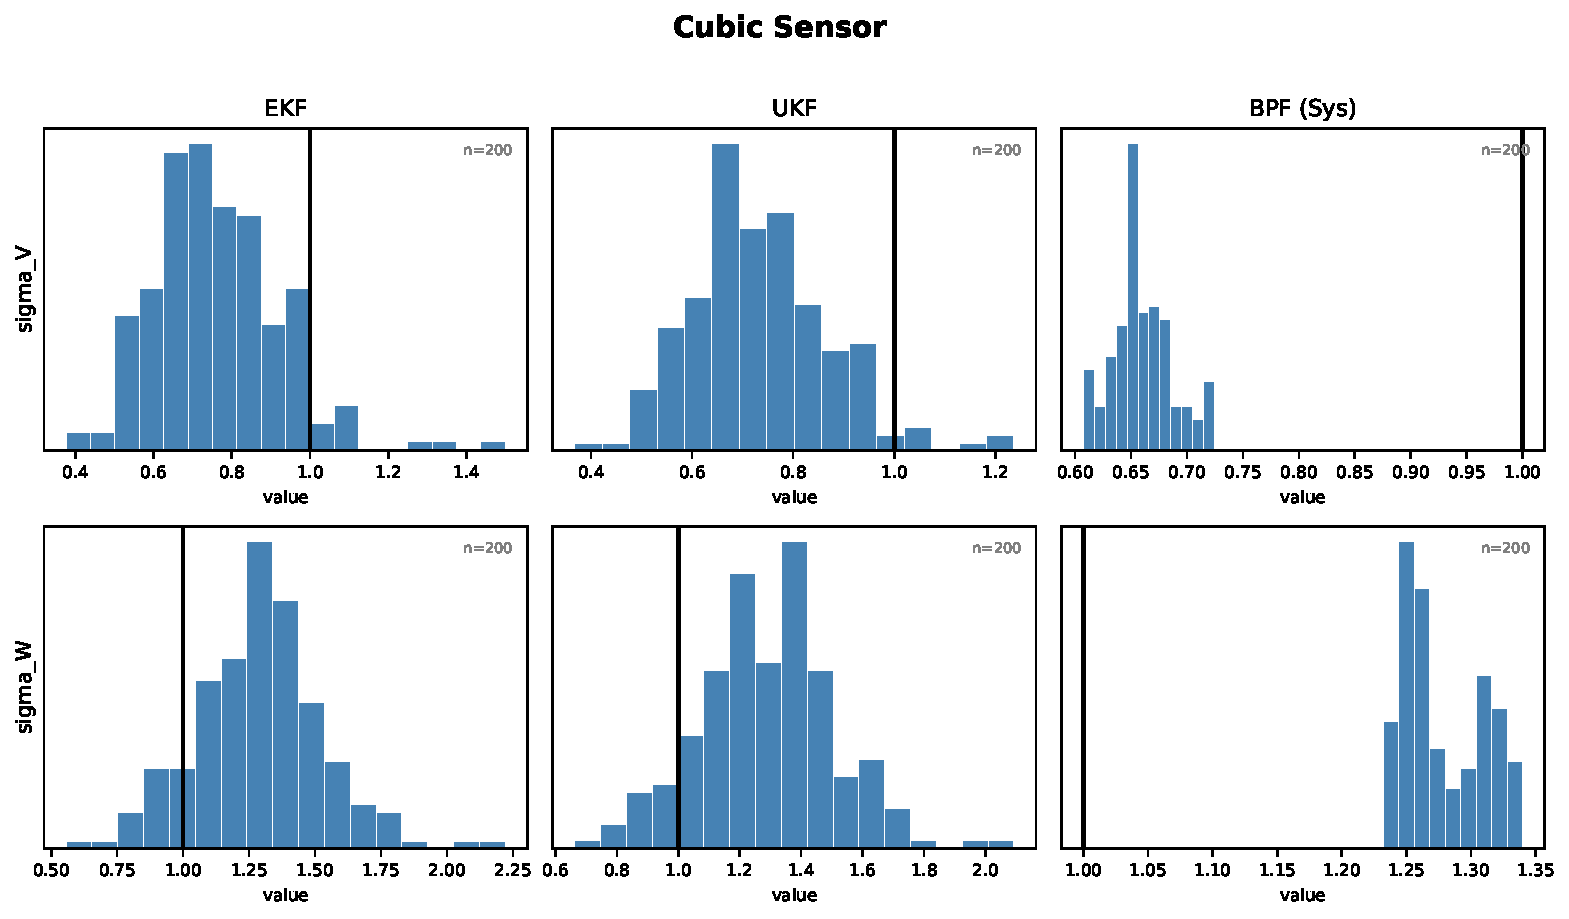
\includegraphics[width=\textwidth]{hmc_cubic_sensor.pdf}
% %     \caption{Cubic Sensor: HMC posteriors across all methods.}
% %     \label{fig:hmc_cubic_sensor}
% % \end{figure}
% 
% % \begin{figure}[H]
% %     \centering
% %     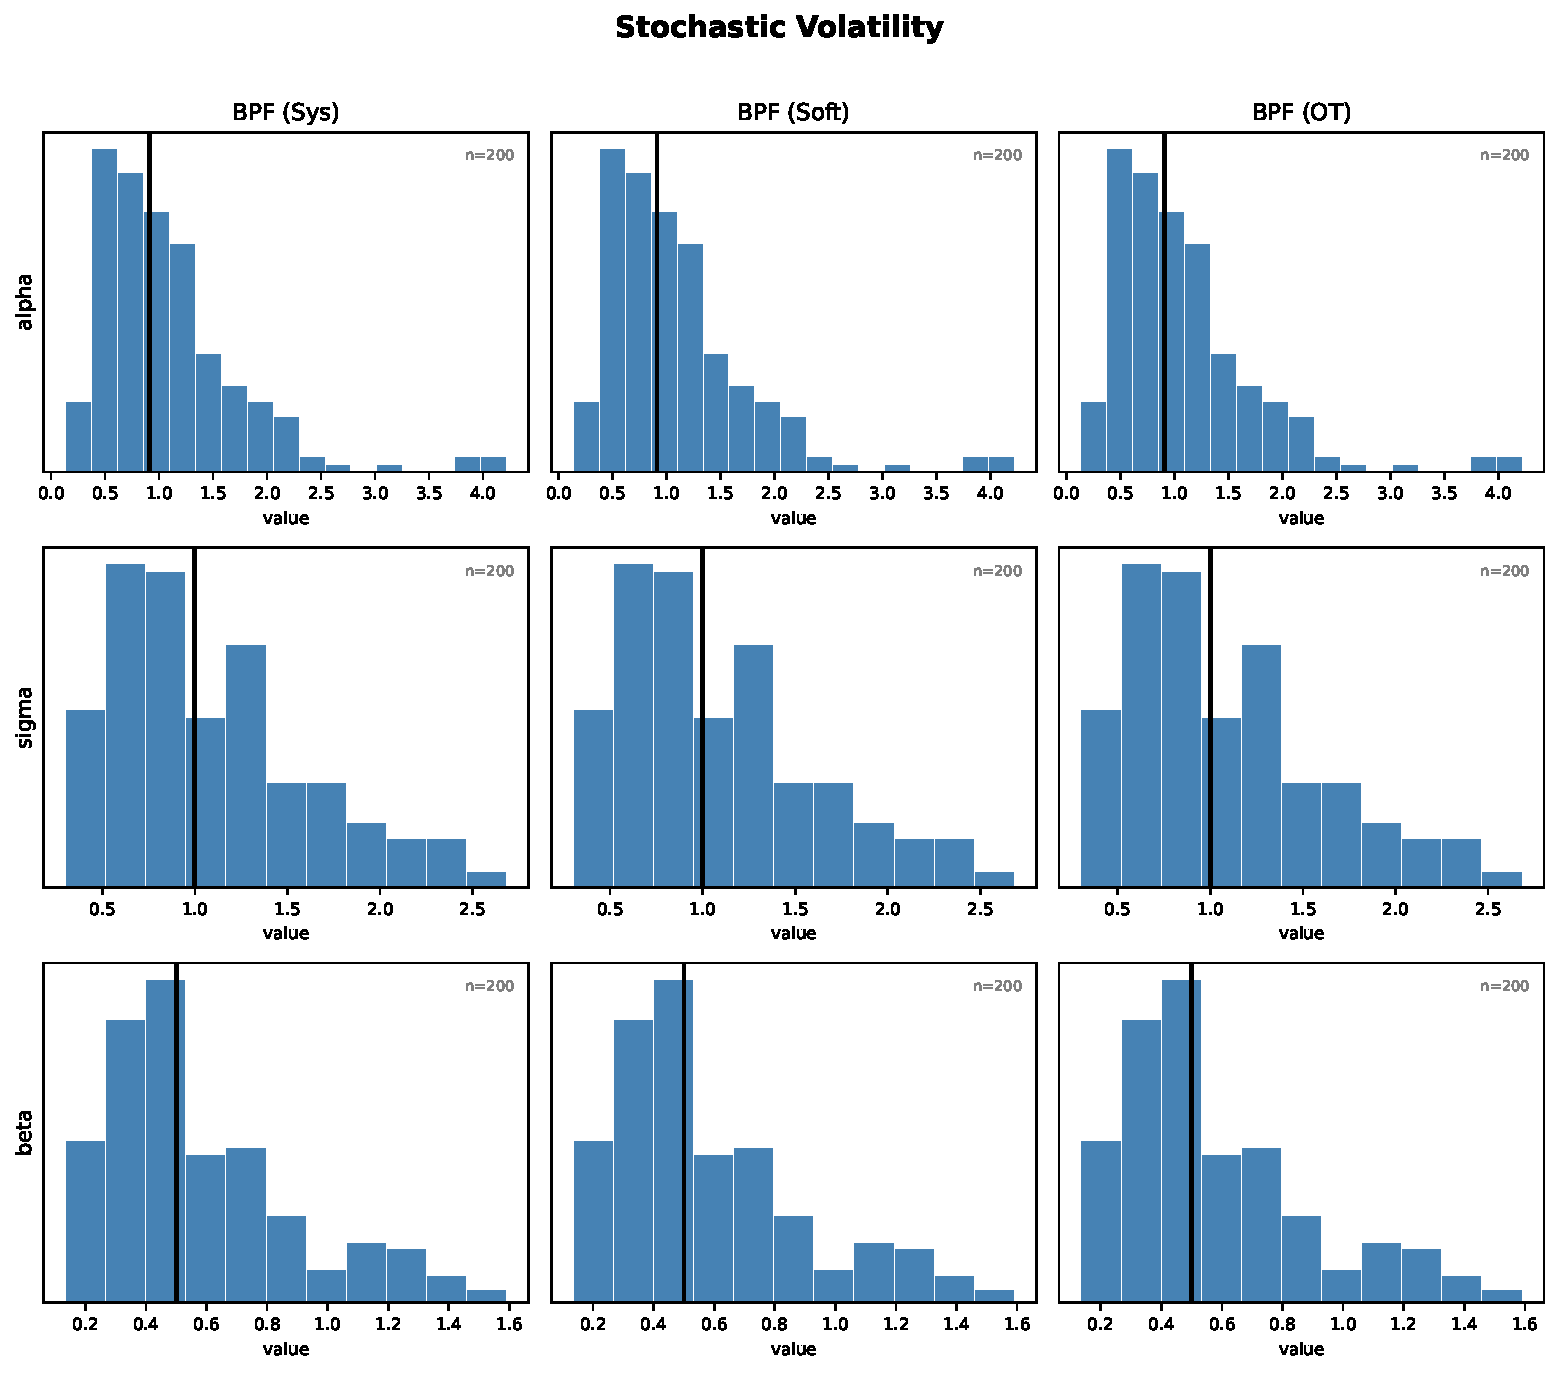
\includegraphics[width=\textwidth]{hmc_stochastic_volatility.pdf}
% %     \caption{Stochastic Volatility: HMC posteriors across BPF methods (systematic, soft, OT resampling).}
% %     \label{fig:hmc_stochastic_volatility}
% % \end{figure}
% 
% 
% Observation: Gradient explosion for any differentiable bootstrap particle filter variation on cubic sensor model. Only thing that stable is the systematic resampling however it will stabilize around the "wrong" minimum. In addition, since anything requiring computing jacobian fails for stochatic volatility model, bpf based method worked really well,  (really fast too). However, the posterior is very wide and provide very little constraint, and resampling methods made absolutely no difference. 
% 
% 
% \subsection{The Kitagawa Model}
% 
% 
% 
% The goal is to build a differentiable particle filter on kitagawa model,
% \begin{equation}
% \begin{split}
% X_n &= \frac{X_{n-1}}{2} + 25 \frac{X_{n-1}}{1 + X_{n-1}^2} + 8 \cos(1.2n) + V_n \\
% Y_n &= \frac{X_n^2}{20} + W_n \\
% \end{split}
% \end{equation}
% where $ X_1 \sim \mathcal{N}(0, 5)$ and
% $ V_n \sim \mathcal{N}(0, \sigma_V^2)$.
% $ W_n \sim \mathcal{N}(0, \sigma_W^2)$, where $\theta=(\sigma_V,\sigma_W)$ is our parameter. The key difficulty is the observation model $Y_n = X_n^2/20 + W_n$: squaring the state destroys sign information, making the filtering distribution bimodal at every time step. Both $+x$ and $-x$ produce the same expected observation $x^2/20$. This means standard filters cannot distinguish the two modes from a single observation, and parameter estimation inherits this structural difficulty. We take a three-step approach:
% \begin{enumerate}
%     \item \textbf{Filtering results.} We first run bootstrap particle filter, LEDH invertible filter on the Kitagawa model to demonstrate that this is a structurally difficult problem. Then we propose an improvement using the observation of the next $k$ step to distinguish the two modes. Even though, it is not always true that most accurate filter is best suitable for Differentiable particle filter, it doesn't hurt to try the improvement then figure out ways to make it compatible with dpf pipeline.
% 
%     \item \textbf{PMCMC paper analysis.} We discuss the approach of Andrieu et al.\cite{Andrieu2010}, who applied Particle Gibbs with a conjugate Inverse Gamma $\theta$-step to this exact model. Their method works, but relies on a conjugate shortcut that is not available for general models. We will report our findings in the actual section.
%  
%      \item \textbf{HMC differentiable particle filter pipeline.} We build a full differentiable pipeline, and report our findings so far, including the difficulties such initialization, comparison between different resampling methods, and how do we plan to improve it further.
%      
%     \end{enumerate}
% 
% 
% 
% Before attempting parameter estimation, we first establish how well various filters track the latent state when the true parameters are known ($\sigma_V^2 = 10$, $\sigma_W^2 = 1$). Table~\ref{tab:kitagawa_filters} summarizes the results for $T = 100$ time steps.
% 
% \begin{table}[H]
% \centering
% \begin{tabular}{lrrrl}
% \toprule
% Filter & $N$ & RMSE & Log-lik & Time (s) \\
% \midrule
% EKF & --- & 33.06 & $-1431.7$ & 1.5 \\
% Bootstrap PF & 1000 & 19.66 & $-360.6$ & 1.4 \\
% EDH Invertible & 500 & 20.67 & $-132.7$ & 18.3 \\
% LEDH Invertible & 500 & 19.91 & $-135.4$ & 15.3 \\
% LEDH Flow & 500 & 18.93 & --- & 14.5 \\
% Bootstrap PF & 10000 & 19.27 & $-359.0$ & 1.3 \\
% LEDH Invertible & 10000 & 19.50 & $-137.0$ & 33.2 \\
% \midrule
% LEDH Bimodal ($K\!=\!1$) & 500 & \textbf{11.57} & $-205.4$ & 18.9 \\
% \bottomrule
% \end{tabular}
% \caption{Filtering performance on Kitagawa model ($T=100$, seed=42, float64). Log-likelihood is the particle filter's estimate of $\log p(z_{1:T})$.}
% \label{tab:kitagawa_filters}
% \end{table}
% 
% Three observations stand out. First, all standard filters (BPF, EDH, LEDH) converge to RMSE $\approx 19$--$21$ regardless of method. The problem is structural: the observation $y = x^2/20$ provides zero sign information, so every filter tracks the magnitude correctly but guesses the sign at chance ($\approx 50\%$). 
% % \begin{figure}[htbp]
% %   \centering
% %   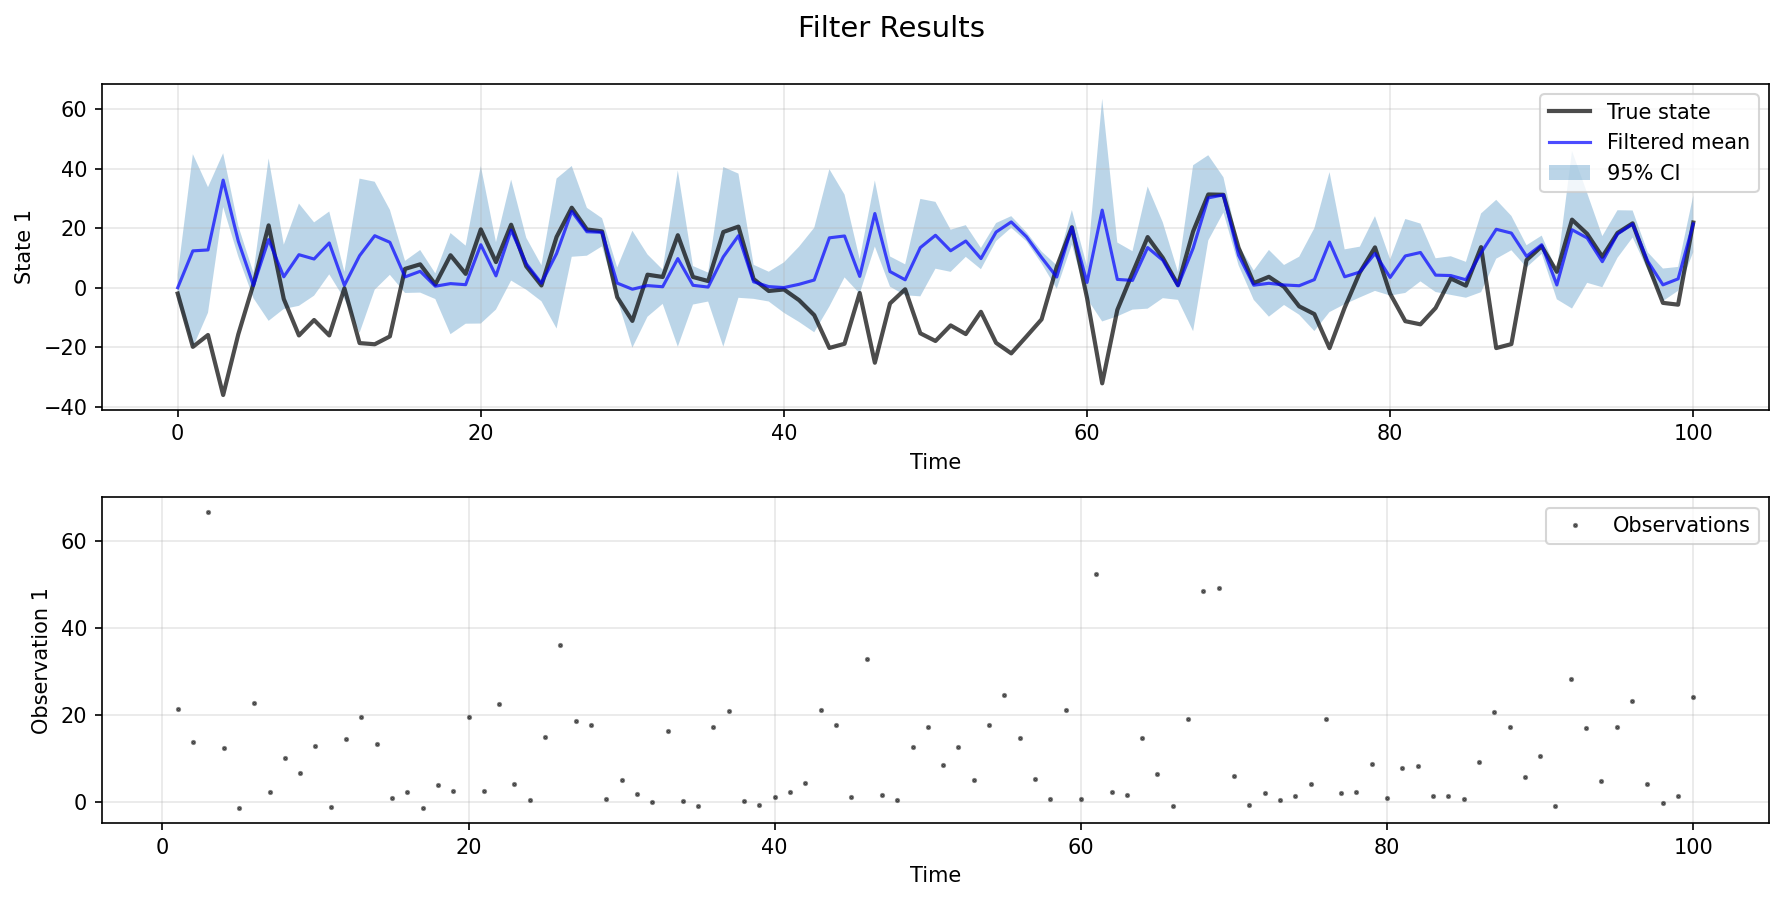
\includegraphics[width=0.9\textwidth]{kitagawa_ledh_1e4.png}
% %   \caption{LEDH invertible filter on the Kitagawa model with 10,000 particles.}
% %   \label{fig:kitagawa_ledh_1e4}
% % \end{figure}
% Second, increasing particles by $20\times$ (from 500 to 10,000) gives less than 1\% RMSE improvement, confirming that the bottleneck is not sample size but the bimodal posterior.Third, the LEDH bimodal filter with a 1-step look-ahead correction (using the next observation $y_{t+1}$ to disambiguate sign via the asymmetric transition dynamics $f(x) \neq f(-x)$) breaks through to RMSE 11.57, a 42\% improvement. 
% % \begin{figure}[htbp]
% %   \centering
% %   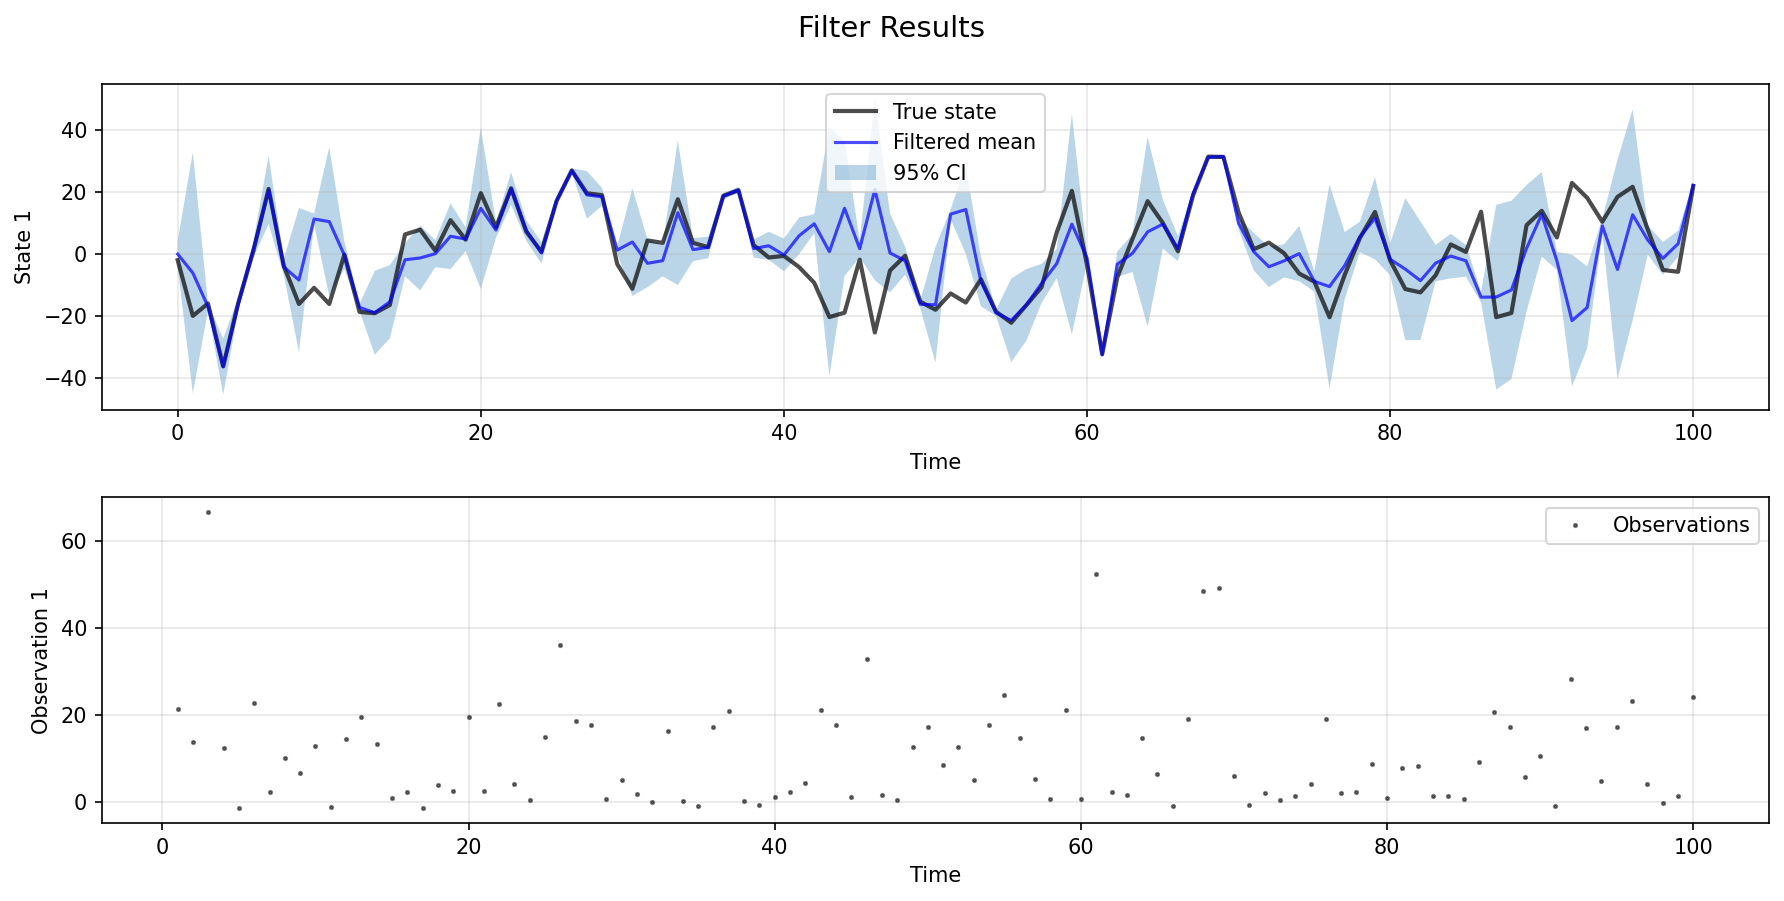
\includegraphics[width=0.9\textwidth]{kitagawa_k1.png}
% %   \caption{LEDH bimodal filter with 1-step look-ahead correction ($k=1$) on the Kitagawa model.}
% %   \label{fig:kitagawa_k1}
% % \end{figure}
% The key insight is that while a single observation $y_t$ cannot distinguish $+x$ from $-x$ (since $h(x) = x^2/20$ is an even function), the \emph{next} observation $y_{t+1}$ can, indirectly. For each flowed particle $\eta_1$, we propagate both signs one step forward through the transition:
% \begin{equation}
% x_{t+1}^{+} = f(+\eta_1,\, t\!+\!1), \qquad x_{t+1}^{-} = f(-\eta_1,\, t\!+\!1),
% \end{equation}
% and compute predicted observations $\hat{y}^{\pm} = (x_{t+1}^{\pm})^2/20$. Because the transition $f(x,t) = x/2 + 25x/(1+x^2) + 8\cos(1.2t)$ contains the even cosine term $8\cos(1.2t)$, we have $f(+x) \neq -f(-x)$ in general, so the two predicted observations differ. Comparing $\hat{y}^+$ and $\hat{y}^-$ against the actual $y_{t+1}$ tells us which sign is more consistent with the data. The flip probability is
% \begin{equation}
% P_{flip} = \sigma\!\Big(\log p(y_{t+1} \mid x_{t+1}^{-}) - \log p(y_{t+1} \mid x_{t+1}^{+})\Big),
% \end{equation}
% where the log-likelihoods use a predictive variance that accounts for process noise propagated through the observation Jacobian. For example, at $t = 50$, we have $\cos(1.2 \times 51) \approx -0.95$:
% \begin{alignat*}{2}
% f(+15) &= 7.5 + 1.66 - 7.6 = 1.56 &\quad&\Longrightarrow\quad \hat{y}^{+} = 1.56^2/20 = 0.12, \\
% f(-15) &= -7.5 - 1.66 - 7.6 = -16.76 &\quad&\Longrightarrow\quad \hat{y}^{-} = 16.76^2/20 = 14.05.
% \end{alignat*}
% If $y_{t+1} \approx 14$, the negative mode is overwhelmingly favored (signal difference $\sim 14$ vs $\sim 0.1$). Table~\ref{tab:kitagawa_ksweep} shows how the look-ahead depth $K$ affects performance.
% 
% \begin{table}[H]
% \centering
% \begin{tabular}{rrrrl}
% \toprule
% $K$ & RMSE & Log-lik & Mean ESS & Time (s) \\
% \midrule
% 0 (baseline) & 19.91 & $-135.4$ & $\sim\!200$ & 12.0 \\
% 1 & \textbf{11.57} & $-205.4$ & 170.8 & 18.9 \\
% 2 & 12.89 & $-215.2$ & 211.2 & 37.1 \\
% 5 & 11.80 & $-196.2$ & 223.5 & 21.3 \\
% 7 & 15.35 & $-208.4$ & 218.4 & 22.3 \\
% 10 & 17.19 & $-214.7$ & 233.6 & 24.0 \\
% \bottomrule
% \end{tabular}
% \caption{LEDH Bimodal look-ahead depth sweep ($N=500$, $n_\lambda=29$, $T=100$, seed=42, float64).}
% \label{tab:kitagawa_ksweep}
% \end{table}
% 
% $K=1$ is already near-optimal (RMSE 11.57, a 42\% improvement over baseline). One step of deterministic propagation through $f(x,t)$ is already asymmetric enough to provide strong discriminative signal. For $K \geq 5$, the deterministic rollout ignores process noise ($\sigma_V = 10$), so later predictions diverge from reality and contribute noise rather than signal to the score. The degradation at $K = 7$ and $K = 10$ confirms this. $K = 1$ is preferred for its simplicity, lowest wall time, and best RMSE. In addition, we note that RMSE and log-likelihood do not follow the same trend. The standard LEDH invertible has the best log-likelihood ($-135$) despite mediocre RMSE ($19.9$): all particles concentrate in one mode, producing well-calibrated weights but a biased point estimate. The bimodal filter spreads particles across both modes, improving the point estimate (lower RMSE) but diluting the predictive density (lower log-likelihood). This dissociation is characteristic of bimodal filtering problems.
% 
% 
% We keep in mind that  \textbf{the sign correction is not differentiable.}
% The look-ahead scoring produces a smooth flip probability $p_{\text{flip}} = \sigma(\cdot)$ via the sigmoid, but the actual flip decision uses a hard threshold which means if we wanted to embed this filter inside a differentiable particle filter framework---learning $\theta$ by minimizing $-\log p(y_{1:T} \mid \theta)$ via gradient descent through the entire filter---the sign correction would block gradients. The loss would not see the effect of $\theta$ on the sign decisions. In the future, we can try to replace the hard threshold with a soft threshold, or other novel improvement. 
% 
% 
% %%%%%%%%%%%%%%%%%%%%%%%%%%%%%%%%%%%%%%%%%%%%%%%%%%%%%%%%%%
% \newpage
% \appendix
% 
% \section{Benchmark Models}\label{app:benchmark_models}
% 
% 
% We first list all the models that I have used in the numerical experiments.
% \begin{enumerate}
% 
% \item \textbf{Linear-Gaussian Model}
% 
% Dynamics:
% \[ X_n = F \cdot X_{n-1} + B \cdot V_n, \quad V_n \sim \mathcal{N}(0, I) \]
% 
% Observation:
% \[ Y_n = H \cdot X_n + D \cdot W_n, \quad W_n \sim \mathcal{N}(0, I) \]
% 
% Parameters:
% \begin{itemize}
% \item $F \in \mathbb{R}^{n_x \times n_x}$: State transition matrix
% \item $B \in \mathbb{R}^{n_x \times n_v}$: Process noise matrix
% \item $H \in \mathbb{R}^{n_y \times n_x}$: Observation matrix
% \item $D \in \mathbb{R}^{n_y \times n_w}$: Observation noise matrix
% \item $Q = BB^T$: Process noise covariance
% \item $R = DD^T$: Observation noise covariance
% \end{itemize}
% This is the simplest benchmark model for filtering. 
% 
% 
% \item \textbf{Acoustic Tracking Full Model (4 targets, 25 sensors)}
% 
% Dynamics (4 independent targets):
% \[ X_{t+1} = F X_t + w_t, \quad w_t \sim \mathcal{N}(0, V) \]
% where $F \in \mathbb{R}^{16 \times 16}$ is block diagonal with 4 identical blocks, $X \in \mathbb{R}^{16}$
% 
% Observation (additive amplitude):
% \[ z_s = \sum_{i=1}^{4} \frac{\Psi}{r_{s,i}^2 + d_0} + \epsilon_s, \quad \epsilon_s \sim \mathcal{N}(0, \sigma_w^2) \]
% 
% Parameters:
% \begin{itemize}
% \item $V_{\text{true}} = \frac{1}{20} \text{diag}(V_{\text{single}}, \ldots, V_{\text{single}})$ (4 blocks)
% \item $V_{\text{filter}} = \text{diag}(\begin{bmatrix} 3 & 0 & 0.1 & 0 \\ 0 & 3 & 0 & 0.1 \\ 0.1 & 0 & 0.03 & 0 \\ 0 & 0.1 & 0 & 0.03 \end{bmatrix}, \ldots)$ (4 blocks)
% \item $\Psi = 10, d_0 = 0.1, \sigma_w = 0.1$
% \item Sensors: $5 \times 5$ grid on $[0, 40] \times [0, 40]$. Basically evenly spread out in the whole area. 
% \end{itemize}
% 
% 
% 
% 
% \item \textbf{Range-Bearing Model}
% 
% Dynamics:
% \[ X_t = F X_{t-1} + w_t, \quad w_t \sim \mathcal{N}(0, Q), \quad X = [x, y]^T \]
% 
% Observation (nonlinear):
% \[ \begin{bmatrix} \text{range} \\ \text{bearing} \end{bmatrix} = \begin{bmatrix} \sqrt{(x - x_s)^2 + (y - y_s)^2} \\ \arctan2(y - y_s, x - x_s) \end{bmatrix} + \begin{bmatrix} v_r \\ v_b \end{bmatrix} \]
% where $v_r \sim \mathcal{N}(0, \sigma_r^2), v_b \sim \mathcal{N}(0, \sigma_b^2)$
% 
% Parameters:
% \begin{itemize}
% \item $F$: State transition (default: identity)
% \item $Q$: Process noise covariance (default: $0.01 I_2$)
% \item $(x_s, y_s)$: Sensor position (default: origin)
% \item $\sigma_r = 0.1$: Range noise std
% \item $\sigma_b = 0.01$: Bearing noise std (radians)
% \end{itemize}
% 
% \item \textbf{Two-Sensor Bearing-Only Model}
% 
% Dynamics (static):
% \[ X_{t+1} = X_t, \quad X = [x, y]^T \]
% 
% Observation:
% \[ \begin{bmatrix} \text{bearing}_1 \\ \text{bearing}_2 \end{bmatrix} = \begin{bmatrix} \arctan2(y - y_{s,1}, x - x_{s,1}) \\ \arctan2(y - y_{s,2}, x - x_{s,2}) \end{bmatrix} + \begin{bmatrix} v_1 \\ v_2 \end{bmatrix} \]
% where $v_i \sim \mathcal{N}(0, \sigma_b^2)$
% 
% Parameters:
% \begin{itemize}
% \item Prior: $\mu_0 = [3.0, 5.0]^T, \Sigma_0 = \begin{bmatrix} 1000 & 0 \\ 0 & 2 \end{bmatrix}$ (highly anisotropic)
% \item Sensors: $[(3.5, 0), (-3.5, 0)]$
% \item $\sigma_b = 0.2$: Bearing noise std
% \item $R = \text{diag}(0.04, 0.04)$
% \end{itemize}
% 
% \item \textbf{Stochastic Volatility Model}
% 
% Dynamics (linear):
% \[ x_t = \alpha x_{t-1} + \sigma w_t, \quad w_t \sim \mathcal{N}(0, 1) \]
% 
% Observation (nonlinear, non-Gaussian):
% \[ y_t = \beta \exp(x_t/2) v_t, \quad v_t \sim \mathcal{N}(0, 1) \]
% 
% Parameters:
% \begin{itemize}
% \item $\alpha = 0.91$: Persistence parameter
% \item $\sigma = 1.0$: Volatility of volatility
% \item $\beta = 0.5$: Scale parameter
% \item Stationary variance: $\sigma^2/(1 - \alpha^2)$
% \end{itemize}
% 
% \item \textbf{Lorenz 96 Model}
% 
% Dynamics (chaotic, high-dimensional):
% \[ \frac{dx_i}{dt} = (x_{i+1} - x_{i-2}) x_{i-1} - x_i + F \]
% with cyclic boundary conditions, integrated using 4th-order Runge-Kutta
% 
% Observation (linear, sparse):
% \[ Y = H X + \epsilon, \quad \epsilon \sim \mathcal{N}(0, R) \]
% where $H$ observes every 4th variable
% 
% Parameters:
% \begin{itemize}
% \item $n_x = 1000$: State dimension
% \item $F = 8.0$: Forcing constant (chaotic regime)
% \item $\Delta t = 0.05$: Integration time step
% \item Observation interval: every 20 RK4 steps
% \item $\sigma_{\text{obs}} = 1.0$: Observation noise std
% \item $R = I_{n_y}$, where $n_y = 250$ (25\% observed)
% \end{itemize}
% \item Kitagawa Model(Model from \cite{Andrieu2010})
% \begin{equation}
% \begin{split}
% X_n &= \frac{X_{n-1}}{2} + 25 \frac{X_{n-1}}{1 + X_{n-1}^2} + 8 \cos(1.2n) + V_n \\
% Y_n &= \frac{X_n^2}{20} + W_n \\
% \end{split}
% \end{equation}
% where $ X_1 \sim \mathcal{N}(0, 5)$ and
% $ V_n \sim \mathcal{N}(0, \sigma_V^2)$ \\
% $ W_n \sim \mathcal{N}(0, \sigma_W^2)$, where $\theta=(\sigma_v,\sigma_W)$ is our parameter. We only need to estimate the noise scale while the observation and dynamics are fixed.
% 
% \item \textbf{Cubic Sensor Model}
% 
% Dynamics (linear AR(1)):
% \[ x_t = a \, x_{t-1} + v_t, \quad v_t \sim \mathcal{N}(0, \sigma_V^2) \]
% 
% Observation (mildly nonlinear):
% \[ y_t = x_t + c \, x_t^3 + w_t, \quad w_t \sim \mathcal{N}(0, \sigma_W^2) \]
% 
% Parameters:
% \begin{itemize}
% \item $a = 0.9$: AR coefficient
% \item $c = 0.05$: Cubic nonlinearity strength
% \item $\sigma_V = 1.0$: Process noise std
% \item $\sigma_W = 1.0$: Observation noise std
% \item Initial distribution: $x_0 \sim \mathcal{N}(0, 5)$
% \end{itemize}
% The observation function $h(x) = x + cx^3$ has Jacobian $1 + 3cx^2 > 0$ everywhere, so it is injective. Setting $c = 0$ recovers the linear-Gaussian model. This makes it a useful stepping stone between the linear-Gaussian benchmark and the more challenging Kitagawa model: nonlinear enough to require a particle filter, but tame enough that debugging the pipeline is not a headache.
% 
% \end{enumerate}
% \section{Code Organization}\label{app:code_org}
% 
% 
% \subsection{Configuration Management}
% We use Hydra to manage the configuration with yaml files. Hydra is a framework that allows flexible management of the configurations. We start with a default base configuration for model and filters. In practice, we can override the default configuration with new configurations easily and the output file will automatically save a copy of the overwritten version of the configuration. In this way, we can easily create new experiments while keep track of the parameters corresponding to individual experiment outcome.
% \subsection{Code Base Organization}
% 
% The codebase follows a modular design where models, filters, and experiment infrastructure are kept independent from each other. The motivation is simple: in filtering research, we constantly need to mix and match different filters with different models. If the model logic and filter logic are entangled, adding a new filter or testing an existing one on a new model becomes unnecessarily painful. By separating these concerns, we can, for instance, run all twenty filters on the linear Gaussian model with a one-line config change.
% 
% The source code lives under \texttt{src/} and is organized into the following modules:
% \begin{itemize}
%     \item \texttt{core/} defines the abstract interfaces that the rest of the code builds on. \texttt{StateSpaceModel} specifies what any model must provide: sampling methods for state transitions and observations, log-probability evaluations for particle filters, and Jacobians for the EKF/UKF family. \texttt{Filter} defines a common filtering interface with \texttt{predict()}, \texttt{update()}, and \texttt{filter()} methods. All concrete implementations inherit from these base classes. This means that every model works with every filter without special-casing, and a new model or filter only needs to implement the abstract interface to integrate with the full pipeline.
%     \item \texttt{models/} contains the concrete state-space models. We have ten models ranging from the standard 2D linear Gaussian (which serves as our ground truth benchmark) to highly nonlinear ones like stochastic volatility and range-bearing tracking. Each model provides both a NumPy interface (used by Kalman filters) and a TensorFlow interface (used by particle filters and differentiable methods). The dual interface is necessary because Kalman filters operate on matrices directly while particle filters need batch-vectorized tensor operations for GPU acceleration.
%     \item \texttt{filters/} is split into \texttt{kalman/} and \texttt{particle/}. The Kalman side is relatively simple: a standard Kalman filter (with Joseph form for numerical stability), an Extended Kalman Filter, and an Unscented Kalman Filter. The particle side is where the bulk of the research code lives, with eighteen implementations spanning bootstrap particle filters, kernel-based flow filters, the Exact Daum-Huang family (global and local variants), invertible flow filters with importance weighting, and conditional SMC. A shared base class \texttt{ParticleFilterBase} handles diagnostic tracking --- ESS history, weight distributions, resampling events --- so that every particle filter automatically records the quantities we need for debugging and analysis. With filters inherit structure from easier filter, such as stochastic flow filter inherits from Exact-Duam-Huang flow filter, we only have to debug the updated methods instead of the whole class.
%     
%     \item \texttt{resampling/} provides three resampling strategies: systematic resampling (the standard low-variance method), soft resampling (a continuous relaxation that avoids hard index selection, useful for differentiable settings), and optimal transport entropy resampling. Each method follows the same interface, so swapping resampling methods is a config-level change.
%     \item \texttt{utils/} provides the numerical building blocks that the rest of the code depends on. For example, numerically stable linear algebra and other supporting function that is repeated called by other filters.
%       \item \texttt{experiments/} contains the Hydra-based experiment runner. Given a YAML configuration specifying the model, filter, and parameters, it instantiates the objects, runs the filter, generates diagnostic plots, and records timing and memory statistics. The outputs are saved alongside a copy of the resolved configuration, so every experiment result can be traced back to the exact parameters that produced it.
%     \item \texttt{DF/} houses the differentiable filtering module for parameter estimation. This includes runners for Hamiltonian Monte Carlo (HMC), Particle Gibbs (PGibbs), and Particle Marginal Metropolis-Hastings (PMMH). The idea is that once we have a working particle filter, we can treat the log-likelihood it computes as a differentiable function of the model parameters and use gradient-based or MCMC methods to fit those parameters to data.
% \end{itemize}
% 
% \section{Testing Strategy}\label{app:testing}
% 
% 
% 
% Every test fixes the random seed, so the output is deterministic. There is no stochasticity to deal with. The anchor for all filter tests is the 2D linear-Gaussian model with a Kalman filter, which gives the exact posterior mean, covariance, and log-likelihood at every time step. We run each particle filter on the same model and same observations, then check that the posterior mean converges to the Kalman solution and the log-likelihood is within tolerance. All three resampling methods (systematic, soft, OT) are tested independently this way. We also check numerical health --- no NaN or Inf in weights, ESS never collapsing, particles not degenerating to a single point --- and edge cases like running with only 10 particles or with extremely tight observation noise.
% 
% The resampling methods are tested in isolation, outside of any filter. For systematic resampling: selection frequency matches the weights, uniform weights produce an exact permutation, and degenerate weights correctly duplicate a single particle. For soft resampling: $\alpha = 1$ reduces to systematic, $\alpha = 0$ gives uniform sampling, and output weights always sum to one. For OT: output weights are finite, and uniform input weights produce near-identity transport. All three methods are stress-tested with extreme weight ratios. The linear algebra utilities and ODE solvers have their own unit tests against known analytical solutions.
% 
% 
% 
% \newpage
% [Appendix D moved into Section: Benchmark Linear Gaussian Model]% 
% \section{MCMC Diagnostics}\label{app:mcmc_diagnostics}
% 
% This appendix details the four diagnostic quantities reported after every HMC run.
% 
% \subsection{Acceptance Rate}
% 
% At each HMC step a proposal $q^*$ is drawn by integrating Hamilton's equations for $L$ leapfrog
% steps from the current state $q$.  The joint state is $(q, p)$ where $p \sim \mathcal{N}(0, I)$ is
% the auxiliary momentum.  The \emph{Hamiltonian} is
% \begin{equation}
%   H(q, p) = -\log \pi(q) + \tfrac{1}{2}\|p\|^2,
% \end{equation}
% where $\pi(q)$ is the target density (here the posterior).  The Metropolis acceptance probability is
% \begin{equation}
%   \alpha = \min\!\left(1,\; e^{-\Delta H}\right), \qquad
%   \Delta H = H(q^*, p^*) - H(q, p).
% \end{equation}
% If the leapfrog integrator were exact, $\Delta H = 0$ and every proposal would be accepted.
% Numerical discretisation error causes $\Delta H \neq 0$, so some proposals are rejected.
% 
% \paragraph{Example.}
% Suppose $\Delta H = 0.5$.  Then $\alpha = e^{-0.5} \approx 0.607$, i.e.\ the proposal is accepted
% with probability~61\%.  If $\Delta H < 0$ (proposal has lower energy / higher probability), the
% proposal is always accepted.
% 
% \paragraph{Target acceptance rate.}
% For standard HMC, the theoretically optimal acceptance rate in high dimensions is approximately
% $0.65$~\cite{beskos2013optimal}.  For NUTS and problems with smoother posteriors, a higher target
% of $0.80$--$0.90$ is common.  Acceptance rates near $100\%$ indicate the step size is too small:
% proposals barely move and consecutive samples are highly correlated.
% 
% \subsection{Step Size and Dual-Averaging Adaptation}
% 
% The leapfrog step size $\varepsilon$ controls how far each sub-step moves in parameter space.
% A total HMC trajectory covers approximately $L\varepsilon$ in unconstrained space.  Too large
% $\varepsilon$ causes large $\Delta H$ and frequent rejection; too small $\varepsilon$ gives
% near-certain acceptance but slow exploration.
% 
% The step size is adapted during burn-in using \emph{dual averaging} (Hoffman \& Gelman,
% 2014~\cite{hoffman2014nuts}), which is the same algorithm used in our custom HMC implementation
% (\texttt{hmc\_runner.py}).  Let $\delta$ be the target acceptance probability and $\alpha_m$ the
% actual acceptance probability at step $m$.  The update equations are:
% \begin{align}
%   \bar{H}_m &= \left(1 - \frac{1}{m + t_0}\right)\bar{H}_{m-1}
%               + \frac{1}{m + t_0}(\delta - \alpha_m),
%               \label{eq:da_hbar}\\[4pt]
%   \log \varepsilon_m &= \mu - \frac{\sqrt{m}}{\gamma}\,\bar{H}_m,
%               \label{eq:da_eps}\\[4pt]
%   \log \bar{\varepsilon}_m &= m^{-\kappa}\log \varepsilon_m
%               + (1 - m^{-\kappa})\log \bar{\varepsilon}_{m-1}.
%               \label{eq:da_epsbar}
% \end{align}
% Here $\mu = \log(10\varepsilon_0)$ is a free target (set to $10\times$ the initial step size),
% $\gamma = 0.05$ is a shrinkage factor, $t_0 = 10$ stabilises early iterations, and $\kappa = 0.75$
% controls the long-run averaging weight.  The \emph{running average} $\bar{\varepsilon}_m$ is
% used as the final step size after adaptation ends; this is more stable than the instantaneous
% $\varepsilon_m$.  In our code the adaptation runs for the first $80\%$ of burn-in steps.
% 
% \paragraph{Intuition.}
% When $\alpha_m < \delta$ the chain is rejecting too often, so $\bar{H}_m$ increases and
% Eq.~\eqref{eq:da_eps} decreases $\varepsilon$.  When $\alpha_m > \delta$ the opposite happens.
% The exponential averaging in Eq.~\eqref{eq:da_epsbar} smooths out this feedback.
% 
% \subsection{Effective Sample Size}
% 
% Because consecutive MCMC samples are correlated, $N$ correlated samples carry less information
% than $N$ independent ones.  The \emph{effective sample size} (ESS) quantifies how many
% independent samples the chain is equivalent to:
% \begin{equation}
%   \mathrm{ESS} = \frac{N}{1 + 2\displaystyle\sum_{k=1}^{\infty} \rho_k},
% \end{equation}
% where $\rho_k = \mathrm{Corr}(\theta_t, \theta_{t+k})$ is the lag-$k$ autocorrelation of the
% chain.  In practice the infinite sum is truncated where the autocorrelations become negligible.
% Our implementation calls \texttt{tfp.mcmc.effective\_sample\_size}, which estimates the sum via
% FFT-based autocorrelation.
% 
% \paragraph{Demonstration: AR(1) chain.}
% Suppose $\theta_t = \phi\,\theta_{t-1} + \varepsilon_t$ with $|\phi| < 1$.  Then
% $\rho_k = \phi^k$, and the geometric series gives
% \begin{equation}
%   \mathrm{ESS} = N\,\frac{1 - \phi}{1 + \phi}.
% \end{equation}
% \begin{center}
% \begin{tabular}{ccc}
% \toprule
% Autocorrelation $\phi$ & $N = 200$ samples & ESS \\
% \midrule
% $0.0$ & 200 & $200$ \quad (independent) \\
% $0.5$ & 200 & $67$ \\
% $0.9$ & 200 & $\approx 11$ \quad (poor mixing) \\
% $0.99$ & 200 & $\approx 1$ \quad (stuck) \\
% \bottomrule
% \end{tabular}
% \end{center}
% 
% \paragraph{Reliability.}
% With only $N = 200$ post-burn-in samples the autocorrelation estimator is itself noisy.  The
% FFT-based estimator can underestimate the true autocorrelation, causing ESS to saturate at $N$
% even when mixing is imperfect.  ESS estimates require at least several hundred samples to be
% trustworthy.
% 
% \subsection{$\hat{R}$: Potential Scale Reduction Factor}
% 
% The $\hat{R}$ statistic (Gelman \& Rubin, 1992) compares \emph{within-chain} variance to
% \emph{between-chain} variance to detect non-convergence.  Since we run a single chain, we follow
% the common practice of splitting the $N$ post-burn-in samples into two halves of length
% $n = N/2$ each, treating them as independent chains ($m = 2$).
% 
% Let $\bar\theta_j$ and $s_j^2$ be the mean and variance of chain $j$.  Define
% \begin{align}
%   W &= \frac{1}{m}\sum_{j=1}^{m} s_j^2
%   && \text{(within-chain variance)}, \\[4pt]
%   B &= \frac{n}{m-1}\sum_{j=1}^{m}(\bar\theta_j - \bar{\bar\theta})^2
%   && \text{(between-chain variance)}, \\[4pt]
%   \hat{V} &= \frac{n-1}{n}\,W + \frac{1}{n}\,B
%   && \text{(pooled variance estimate)}.
% \end{align}
% Then
% \begin{equation}
%   \hat{R} = \sqrt{\frac{\hat{V}}{W}}.
% \end{equation}
% 
% \paragraph{Interpretation.}
% If the chain has converged, both halves should look like draws from the same stationary
% distribution, so $B \approx 0$ and $\hat{V} \approx W$, giving $\hat{R} \approx 1$.
% A value $\hat{R} > 1.1$ is the standard threshold for flagging non-convergence.
% 
% \paragraph{Why $\hat{R}$ can be less than 1.}
% Mathematically, $\hat{R} < 1$ requires $\hat{V} < W$, which happens when $B$ is very small
% (the two half-chains have nearly identical means) but $W$ is inflated by within-chain
% fluctuations.  With only $n = 100$ samples per half-chain, both $W$ and $B$ are estimated
% with high uncertainty, and values like $\hat{R} = 0.83$ are consistent with a correctly
% converging chain that simply has too few samples for reliable estimation.  At least
% $n \geq 200$ per chain ($N \geq 400$ total) is recommended before trusting $\hat{R}$.
% 
\bibliographystyle{unsrt}

\bibliography{main_reorganized}
\end{document}
